% ============================================================
%  História do Inferno — Edição Expandida e Complementada
%  Conversão .docx → LaTeX (memoir + babel pt-br)
% ============================================================
\documentclass[11pt,a4paper,openright,twoside]{memoir}

% ---------- Pacotes essenciais ----------
\usepackage[T1]{fontenc}
\usepackage[utf8]{inputenc}
\usepackage[portuguese]{babel}
\usepackage{lmodern}
\usepackage{csquotes}
\usepackage{microtype}
\usepackage{graphicx}
\usepackage{xcolor}
\usepackage{hyperref}
\usepackage[alf,abnt-emphasize=bf,abnt-etal-list=3]{abntex2cite}
\usepackage{etoolbox}
\usepackage{enumitem}
\usepackage{tabularx}
\usepackage{longtable}
\usepackage{array}
\usepackage{caption}
\usepackage{booktabs}

% ---------- Configuração de imagens ----------
\graphicspath{{figuras/}}
\setkeys{Gin}{width=\linewidth,keepaspectratio}

% ---------- Hiperlinks (cores sóbrias) ----------
\hypersetup{
  colorlinks=true,
  linkcolor=red!70!black,
  citecolor=blue!70!black,
  urlcolor=blue!70!black,
  pdftitle={História do Inferno: Edição Expandida e Complementada},
  pdfauthor={Ney Lemke},
  pdfsubject={Análise interdisciplinar da evolução histórica dos conceitos de inferno},
  pdfkeywords={inferno; escatologia; história das religiões; teologia; mitologia}
}

% ---------- Tipografia memoir ----------
% A4 (210x297mm) com margens de livro -- margens internas maiores
% (binding) e externas menores; margens verticais balanceadas.
\linespread{1.15}
\setlrmarginsandblock{2.5cm}{2.0cm}{*}
\setulmarginsandblock{2.8cm}{2.8cm}{*}
\setheadfoot{\onelineskip}{2\onelineskip}
\setheaderspaces{*}{2\onelineskip}{*}
\checkandfixthelayout

% ---------- Cabeçalhos / rodapés ----------
% Estilo custom 'klimt' baseado no ruled: título do capítulo aparece em
% AMBAS as páginas (par e ímpar), número da página fica no rodapé central.
\makepagestyle{klimt}
\makeheadrule{klimt}{\textwidth}{\normalrulethickness}
\makeevenhead{klimt}{\footnotesize\leftmark}{}{}
\makeoddhead{klimt}{}{}{\footnotesize\leftmark}
\makeevenfoot{klimt}{\thepage}{}{}
\makeoddfoot{klimt}{}{}{\thepage}
\makeheadfootruleprefix{klimt}{}{}{}{}
\pagestyle{klimt}

% Define um pagestyle 'plainklimt' para abertura de capítulo: sem header,
% só rodapé com número e título do livro.
\copypagestyle{plainklimt}{plain}
\aliaspagestyle{chapter}{plainklimt}

% Marca de capítulo = alias curto definido em \chapter[alias]{titulo}
% (o memoir usa o alias no TOC e nos headers automaticamente)

% ---------- Epígrafes dos capítulos (ajustadas para A4) ----------
\setlength{\epigraphwidth}{0.65\textwidth}
\renewcommand{\epigraphflush}{flushright}
\renewcommand{\epigraphsize}{\footnotesize}

% ---------- Estilo de capítulo (memoir) ----------
% 'hangnum' tem numero centrado acima do título, dentro da area de texto.
% Acomoda numeros de 1 ou 2 dígitos sem cortar nas bordas.
\chapterstyle{hangnum}
\renewcommand{\chaptitlefont}{\normalfont\Large\scshape}
\renewcommand{\printchaptertitle}[1]{\chaptitlefont\centering\MakeUppercase{#1}}
% Capítulo: garante que o leftmark no cabeçalho só tem o alias curto,
% sem prefixo "Capítulo X" duplicado.
\renewcommand{\chaptermark}[1]{\markboth{#1}{}}

% ---------- Estilo de parte ----------
\renewcommand{\partnamefont}{\normalfont\Large\scshape}
\renewcommand{\partnumfont}{\normalfont\huge\scshape}
\renewcommand{\printparttitle}[1]{\partnamefont\centering\MakeUppercase{#1}}

% ---------- Caption de figuras ----------
\captionsetup{font=small,labelfont={bf,small},labelsep=period,justification=centering}

% ---------- Compilação silenciosa ----------
\setcounter{secnumdepth}{3}
\setcounter{tocdepth}{2}

% ============================================================
%   DOCUMENTO
% ============================================================
\begin{document}

% ---------- Front matter ----------
\frontmatter
% ============================================================
%  Front matter — capa, falsa-capa, dedicatória, epígrafe,
%  resumo, agradecimentos, abreviaturas
% ============================================================

% ---------- Página de rosto ----------
\begin{titlingpage}
\thispagestyle{empty}
\begin{center}
\vspace*{3cm}
{\Huge\scshape História do Inferno\par}
\vspace{0.8cm}
{\Large\slshape Edição Expandida e Complementada\par}
\vspace{2.5cm}
{\large Uma Análise Interdisciplinar dos Conceitos de\\
       Punição Eterna da Pré-História à Era Digital\par}
\vspace{2.0cm}
{\large Baseada em 195 Fontes Acadêmicas Especializadas\par}
\vfill
{\large Ney Lemke\par}
\vspace{1.5cm}
{\small São Paulo --- Botucatu\par}
{\small \the\year\par}
\end{center}
\end{titlingpage}

% ---------- Verso da página de rosto (nota editorial) ----------
\thispagestyle{empty}
\vspace*{2cm}
\begin{quote}
\small
\noindent\textbf{Nota editorial sobre esta edição.}

Esta obra foi convertida automaticamente do formato \texttt{.docx}
para \LaTeX{} (\textit{memoir}, classe de livro) preservando a
hierarquia original de 5 partes e 20 capítulos, além de 83 imagens
extraídas para o diretório \texttt{figuras/}.

Durante a conversão foram identificadas duas inconsistências no
original: (i) o sumário referencia o \emph{Capítulo 4 (Período de
Transição Antiga)}, ausente do corpo do texto; (ii) o \emph{Capítulo
17} aparece no corpo sob dois títulos divergentes (``O Inferno no
divã'' e ``O Inferno Contemporâneo''). A numeração impressa segue o
corpo do manuscrito.
\end{quote}
\vfill
\clearpage

% ---------- Dedicatória ----------
\thispagestyle{empty}
\vspace*{4cm}
\begin{center}
\itshape
``A questão do inferno não é apenas sobre o que nos espera depois da
morte.\\[0.3cm]
É sobre o que somos capazes de fazer \emph{aqui}.''
\end{center}
\clearpage

% ---------- Epígrafe geral ----------
\thispagestyle{empty}
\vspace*{3cm}
\begin{flushright}
\begin{minipage}{0.7\textwidth}
\itshape
Há mais coisas entre o céu e a terra, Horacio,\\
do que sonha a nossa vã filosofia.
\end{minipage}

\hfill --- Shakespeare, \textit{Hamlet}, Ato I, Cena V
\end{flushright}
\vfill
\clearpage

% ---------- Resumo ----------
\chapter*{Resumo}
\addcontentsline{toc}{chapter}{Resumo}

Esta obra apresenta uma análise abrangente e interdisciplinar da
evolução histórica dos conceitos de inferno e punição eterna, desde
as primeiras práticas funerárias da pré-história até as
representações distópicas da era digital. Baseada em 195 fontes
acadêmicas especializadas, a investigação percorre cinco grandes
eixos: (i) as origens e a Antiguidade Clássica, com atenção ao
submundo sumério, egípcio e greco-romano; (ii) as tradições
regionais e culturais, incluindo as mitologias nórdica, celta,
eslava, bizantina e ameríndia; (iii) os desenvolvimentos judaico-cristãos,
do \emph{Sheol} à patrística; (iv) as sínteses medievais e modernas,
do Islã medieval a Dante, da Renascença ao Iluminismo; e (v) a era
contemporânea, com suas manifestações literárias, cinematográficas,
digitais e de gênero.

A tese central sustenta que a ideia de inferno --- longe de ser
monolítica --- é uma construção cultural cumulativa, reelaborada a
cada época conforme as ansiedades e os dil éticos de cada civilização.
A análise dialoga com a história das religiões, a teologia, a
antropologia, a literatura, o cinema e os estudos culturais.

% ---------- Agradecimentos ----------
\chapter*{Agradecimentos}
\addcontentsline{toc}{chapter}{Agradecimentos}

Esta obra resulta de anos de investigação em fontes dispersas por
bibliotecas, manuscritos digitalizados, arquivos e bases de dados
acadêmicas. Agradeço a todos os pesquisadores, tradutores e
bibliotecários que, anonimamente, mantêm viva a memória documental
da humanidade. Em especial, aos colegas da UNESP que, em conversas
informais, ajudaram a amadurecer as hipóteses aqui apresentadas.

% ---------- Lista de abreviaturas (opcional, expandível) ----------
\chapter*{Nota sobre abreviaturas e transliterações}
\addcontentsline{toc}{chapter}{Nota sobre abreviaturas e transliterações}

As transliterações de termos em sânscrito, acádio, hebraico, árabe e
grego seguem convenções padronizadas da literatura acadêmica de
referência. Termos em latim aparecem em \textit{itálico} quando
conservados na forma original; termos gregos seguem o sistema
betacode latino. Para facilitar a consulta, o índice remissivo ao
final do volume remete o leitor tanto à grafia original quanto à
tradução aportuguesada.
\clearpage

% ---------- Sumário ----------
\clearpage
\tableofcontents
\clearpage

% ---------- Corpos (partes/capítulos) ----------
\mainmatter
% ============================================================
%  PARTE I: ORIGENS E ANTIGUIDADE CLÁSSICA
% ============================================================

\part{ORIGENS E ANTIGUIDADE CLÁSSICA}
\partmark{ORIGENS E ANTIGUIDADE CLÁSSICA}

% --- Capítulo 1: Os Primórdios da Punição Eterna ---
\chapter[Primórdios da Punição]{Os Primórdios da Punição Eterna}

\epigraph{Cada civilização que julgou os mortos descobriu primeiro o que fazer com seus corpos. Da argila paleolítica às tumbas reais da Mesopotâmia, dos montículos celtas às catacumbas cristãs, a humanidade enterrou seus mortos em padrões que falavam de continuidade --- e, por espelho, de ruptura. O esqueleto humano, ao ser preparado para a terra, desenhou involuntariamente a primeira fronteira entre salvação e condenação.}

\section{Introdução: Origens do Além Sombrio}

A ideia de um lugar de punição após a morte --- o que hoje conhecemos como "inferno" --- não surgiu repentinamente em textos religiosos sofisticados, mas emergiu gradualmente através de milênios de desenvolvimento cultural humano. Antes mesmo da escrita, os primeiros humanos já haviam começado a conceber um destino para os mortos, refletindo sobre o que acontece quando cessa o sopro da vida. Este capítulo explora como as primeiras concepções de punição além-túmulo surgiram, não como doutrinas religiosas formalizadas, mas como tentativas de compreender a morte e impor ordem moral ao universo.

\subsection{A Arqueologia da Punição Pós-Morte}

Os vestígios arqueológicos oferecem janelas fascinantes para as crenças pré-históricas sobre o além. Os enterramentos do Paleolítico Superior (40.000-10.000 a.C.) já apresentavam evidências de rituais elaborados, com corpos frequentemente posicionados cuidadosamente, acompanhados de ornamentos, ferramentas e alimentos. Estas práticas sugerem uma crença na continuação da existência além da morte, embora não necessariamente em um sistema de recompensas e punições.


\begin{figure}[ht]
  \centering
  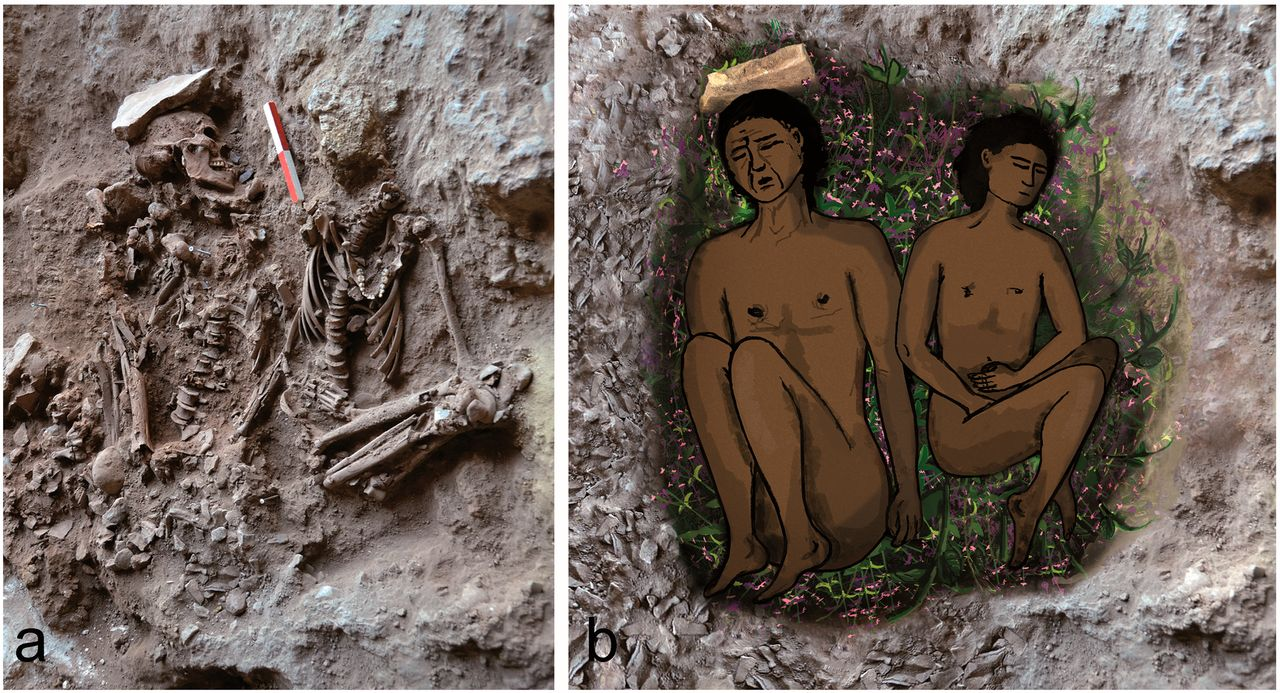
\includegraphics[width=0.85\linewidth]{image1.jpeg}
  \caption{Enterramento paleolítico mostrando disposição ritual de um corpo, indicando crenças primitivas sobre a vida após a morte.}
  \label{fig:cap1-img1}
\end{figure}

Enterramento paleolítico mostrando disposição ritual de um corpo, indicando crenças primitivas sobre a vida após a morte.

Em Çatalhöyük (7500-5700 a.C.), na atual Turquia, pesquisadores encontraram evidências de tratamentos diferenciados para determinados mortos. Enquanto a maioria recebia enterros sob as casas, alguns restos eram expostos a animais necrófagos antes do sepultamento final. Essa diferenciação sugere uma distinção precoce entre "bons" e "maus" mortos, possivelmente refletindo as primeiras concepções de destinos diferenciados após a morte.


\begin{figure}[ht]
  \centering
  \includegraphics[width=0.85\linewidth]{image2.jpeg}
  \caption{Estas práticas constituem as primeiras evidências arqueológicas de uma possível diferenciação de destinos após a morte, um precursor fundamental para o conceito de recompensa e punição no além.}
  \label{fig:cap1-img2}
\end{figure}

Os enterramentos em Çatalhöyük eram frequentemente realizados sob o piso das casas, com os corpos em posição fetal. Estudos arqueológicos recentes revelam que alguns indivíduos recebiam tratamentos diferenciados, sugerindo a existência de hierarquias sociais que poderiam estender-se ao além. A disposição de alguns esqueletos indica que certos indivíduos eram considerados especiais ou, pelo contrário, potencialmente perigosos após a morte.

Estas práticas constituem as primeiras evidências arqueológicas de uma possível diferenciação de destinos após a morte, um precursor fundamental para o conceito de recompensa e punição no além.

As tumbas reais de Ur (2600-2400 a.C.) na Mesopotâmia revelam outro aspecto importante: enterramentos com sacrifícios humanos, onde servidores, músicos e guarda-costas acompanhavam seus senhores na morte. Estas práticas não apenas confirmam a crença em uma continuidade da existência social após a morte, mas também sugerem que esse outro mundo tinha hierarquias e, potencialmente, punições para aqueles que não cumprissem seus papéis.


\begin{figure}[ht]
  \centering
  \includegraphics[width=0.85\linewidth]{image3.jpeg}
  \caption{O ``Poço da Morte'' nas tumbas reais de Ur, mostrando evidências de sacrifícios humanos em larga escala, sugerindo crenças elaboradas sobre a continuidade da hierarquia social no além-mundo.}
  \label{fig:cap1-img3}
\end{figure}

O "Poço da Morte" nas tumbas reais de Ur, mostrando evidências de sacrifícios humanos em larga escala, sugerindo crenças elaboradas sobre a continuidade da hierarquia social no além-mundo.


\section{O Medo dos Mortos: Espíritos Inquietos e Vingativos}

Em muitas culturas primitivas, o medo dos mortos precedeu a crença formal no inferno. Registros etnográficos de sociedades tradicionais mostram uma preocupação universal com o potencial de "espíritos inquietos" causarem problemas aos vivos. Este medo motivava rituais elaborados para garantir que o falecido seguisse pacificamente para o próximo mundo, em vez de permanecer para atormentar os vivos.

As primeiras sepulturas com pedras sobre os cadáveres, encontradas em vários sítios neolíticos (8000-3000 a.C.), possivelmente serviam não apenas para proteger os corpos de animais, mas também para evitar que os mortos "retornassem". Esta prática persistiu em várias culturas, culminando nos enterros de "vampiros" e outros mortos temidos na Europa Medieval, com estacas e outros mecanismos de contenção para impedir que o falecido saísse de seu túmulo.

Desta forma, o primeiro "inferno" pode ter sido simplesmente a condição de espírito insatisfeito e preso ao mundo dos vivos --- uma punição tanto para o falecido quanto para aqueles que permaneciam vivos. O antropólogo Robert Hertz observou que, em muitas culturas tradicionais, a passagem para o além era vista como um processo e não um evento instantâneo, sugerindo que a "condenação" mais antiga pode ter sido ficar preso em um estado intermediário entre a vida e a morte completa.

Os ritos funerários, como o ilustrado, não visavam apenas honrar o morto, mas também garantir sua partida definitiva do mundo dos vivos, evitando assim o estado "infernal" de transição indefinida.

\section{As Primeiras Distinções Morais no Além}

À medida que as sociedades se tornaram mais complexas, também evoluiu a concepção de um julgamento moral após a morte. Os primeiros indícios de uma diferenciação moral no destino pós-morte aparecem em evidências indiretas, como sepultamentos diferenciados para pessoas de status distinto ou mortas em circunstâncias particulares.

O enterro de criminosos em locais separados, sem os ritos funerários adequados, é documentado em várias culturas antigas. Na China do período Shang (1600-1046 a.C.), escavações revelaram esqueletos decapitados e mutilados em fossas comuns, sugerindo que certas mortes eram consideradas impuras ou merecedoras de um destino diferenciado.

Nas culturas megalíticas europeias (4500-1500 a.C.), apenas certas pessoas eram enterradas em túmulos elaborados, indicando uma possível crença em destinos pós-morte distintos com base no status social ou moral. Progressivamente, essas distinções foram se transformando em noções mais explícitas de recompensa e punição baseadas em critérios éticos.


\begin{figure}[ht]
  \centering
  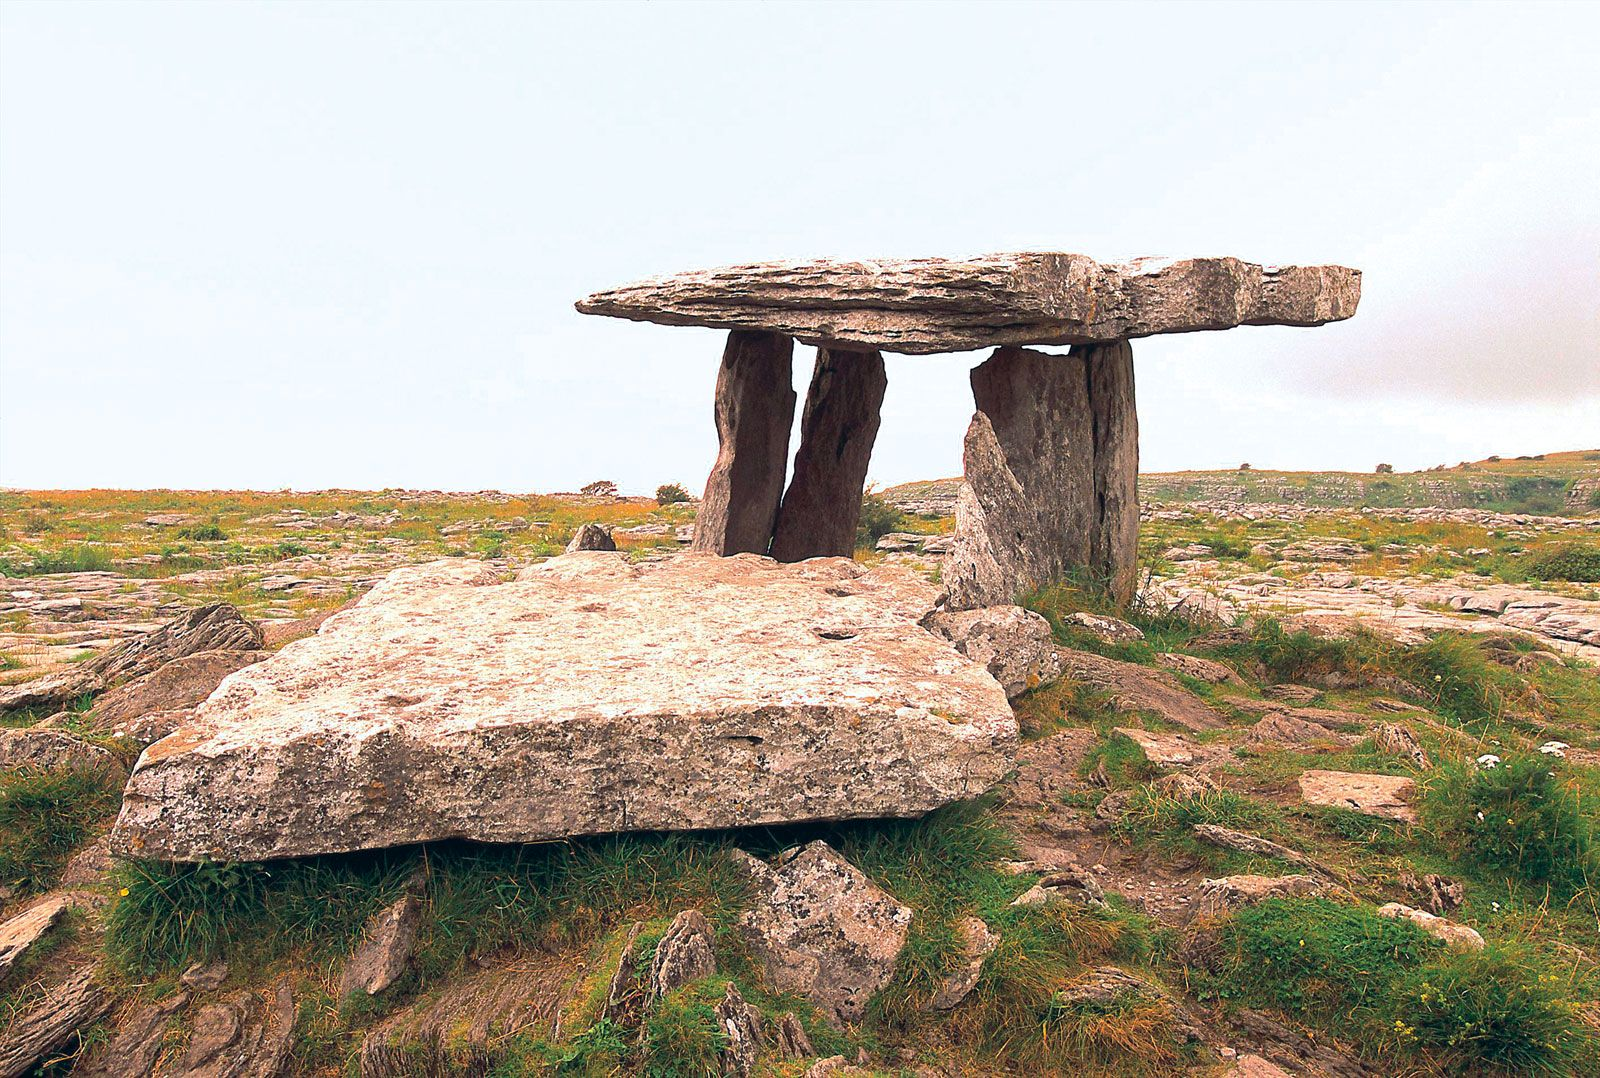
\includegraphics[width=0.85\linewidth]{image4.jpeg}
  \caption{A Geografia Primitiva do Além}
  \label{fig:cap1-img4}
\end{figure}

Dolmen de Poulnabrone na Irlanda, exemplo de tumba megalítica que servia de portal entre o mundo dos vivos e dos mortos. Apenas indivíduos selecionados eram sepultados nestes monumentos impressionantes.

\section{A Geografia Primitiva do Além}

Antes das concepções elaboradas de paraíso e inferno, muitas culturas antigas já desenvolviam uma geografia do além-mundo bastante sofisticada. Para a maioria das primeiras civilizações, o mundo dos mortos era frequentemente localizado em quatro coordenadas simbólicas principais:

\begin{table}[ht]
  \centering
  \small
  \renewcommand{\arraystretch}{1.3}
  \caption{Localizações primordiais do além nas civilizações antigas.}
  \begin{tabularx}{\textwidth}{|>{\raggedright\arraybackslash}p{3.2cm}|>{\raggedright\arraybackslash}p{3.8cm}|X|}
    \hline
    \textbf{Localização} & \textbf{Fundamento simbólico} & \textbf{Tradições representativas} \\
    \hline
    Profundezas da Terra & Associação do submundo com a morte, derivada da prática do enterramento; cavernas profundas, abismos e vulcões vistos como entradas para o reino subterrâneo. & Mesopotâmia (Irkalla), Grécia (Hades), Escandinávia (Helheim), Astecas (Mictlan). \\
    \hline
    Além das Águas & Travessia de um rio, lago ou oceano como rito de passagem; a barca ou barqueiro conduz a alma ao outro mundo. & Egito (barca solar), Grécia (Caronte no Aqueronte), tradições nórdicas e celtas. \\
    \hline
    Regiões Ocidentais & O pôr do sol como metáfora natural da morte; o sol ``morre'' diariamente no oeste, onde situar-se-ia o mundo dos mortos. & Grécia (Campos Elísios no ocidente), tradições celtas e germânicas. \\
    \hline
    Céu ou Estrelas & Destino celestial reservado aos favorecidos pelos deuses; identificação do cosmos superior com a morada dos eleitos. & China (acesso celestial por bondade moral), Egito (estrelas indestrutíveis no norte), tradições uranianas e astrais. \\
    \hline
  \end{tabularx}
\end{table}

Nessas primeiras cosmografias, o "inferno" raramente era concebido como um lugar exclusivo de tormento. Em vez disso, era geralmente um domínio sombrio e desolado, onde todos os mortos, ou ao menos a maioria deles, residiam eternamente. A diferenciação entre destinos "bons" e "ruins" após a morte surgiu posteriormente, com a evolução das estruturas sociais e dos sistemas éticos.

\section{O Surgimento da Justiça Cósmica}

O desenvolvimento de concepções mais elaboradas de punição pós-morte coincide com o surgimento de sociedades estratificadas e complexas. À medida que as civilizações cresciam, enfrentando desigualdades sociais e injustiças aparentes, a ideia de uma retribuição após a morte tornou-se mais atraente.

A noção de equilíbrio cósmico aparece em algumas das primeiras inscrições mesopotâmicas (2700-2500 a.C.). O conceito sumério de nam-tar (destino) sugere que as ações em vida determinavam a sorte de uma pessoa tanto antes quanto depois da morte. Similarmente, os antigos egípcios desenvolveram a concepção da pesagem do coração no julgamento de Osíris, onde aqueles considerados indignos eram devorados por Ammit, um monstro híbrido.


\begin{figure}[ht]
  \centering
  \includegraphics[width=0.85\linewidth]{image5.jpeg}
  \caption{A Materialidade do Sofrimento Pós-Morte}
  \label{fig:cap1-img5}
\end{figure}

O julgamento do morto perante Osíris, como ilustrado no Livro dos Mortos egípcio, representa um dos primeiros sistemas elaborados de justiça cósmica. O coração do falecido era pesado contra a pena de Maat (verdade e ordem cósmica). Se o coração fosse mais pesado devido aos pecados acumulados, o monstro Ammit o devoraria, condenando o morto a uma "segunda morte" -- possivelmente a primeira concepção formal de aniquilação como punição divina.

Estas primeiras ideias de justiça pós-morte não apenas ofereciam conforto para aqueles que sofriam injustiças em vida, mas também serviam como poderosas ferramentas de controle social. A ameaça de punição eterna incentivava a conformidade às normas sociais, mesmo quando escapar da justiça terrena parecia possível.

\section{A Materialidade do Sofrimento Pós-Morte}

As punições imaginadas para os mortos nas culturas primitivas eram notavelmente físicas e concretas. Antes das concepções mais abstratas de sofrimento espiritual, o tormento no além era concebido em termos bastante materiais: fome, sede, frio, escuridão ou dor física.

As primeiras descrições do submundo mesopotâmico, como encontradas no "Descida de Inanna ao Mundo Inferior" (c. 1900-1600 a.C.), retratam um local onde os mortos "comem pó e bebem lama". Similarmente, no Hades grego primitivo, as almas eram vistas como sombras sedentas e famintas, desprovidas dos prazeres da vida.

Esta materialidade do sofrimento reflete um aspecto fundamental da psicologia humana: nossa dificuldade em conceber formas de existência radicalmente diferentes de nossa experiência corpórea. As punições imaginárias do além frequentemente espelhavam as formas de sofrimento conhecidas na vida terrena, apenas intensificadas ou eternizadas.

\section{O Papel dos Sonhos e Visões}

Os sonhos com os mortos e as experiências de quase-morte provavelmente contribuíram significativamente para o desenvolvimento das primeiras concepções do além. Evidências antropológicas de culturas xamânicas sugerem que experiências visionárias eram frequentemente interpretadas como viagens ao mundo dos mortos.

O antropólogo Wade Davis documentou como, em diversas culturas tradicionais, experiências de transe e alteração de consciência eram interpretadas como visitas temporárias ao mundo dos mortos. Estas "testemunhas oculares" frequentemente relatavam não apenas a geografia do além, mas também os tormentos sofridos por certos tipos de falecidos.

Os relatos de visões do inferno aparecem em culturas tão diversas quanto os Inuit do Ártico e os povos da Melanésia, sugerindo que a tendência de elaborar concepções de punição no além pode ser um aspecto universal da cognição humana, possivelmente arraigado em nossas experiências de sonho e estados alterados de consciência.

\section{A Demonização dos Deuses Estrangeiros}

Um desenvolvimento crucial na evolução das concepções de inferno foi a transformação de divindades estrangeiras em demônios e torturadores. À medida que culturas entravam em conflito e uma religião suplantava outra, as antigas divindades frequentemente eram rebaixadas ao status de entidades malignas, presidindo reinos de punição.

Este processo é visível na maneira como os deuses cananeanos, como Baal e Moloch, foram posteriormente demonizados nos textos hebraicos, associados a práticas abomináveis como sacrifício infantil. De modo similar, após a cristianização da Europa, antigos deuses pagãos como Odin e Loki foram frequentemente reinterpretados como demônios ou associados ao inferno cristão.

A transformação de deuses em demônios não apenas ajudava a consolidar a nova ordem religiosa, mas também enriquecia a mitologia do inferno, fornecendo personagens complexos e já familiares para povoar o imaginário do além sombrio.


Ao final deste capítulo, torna-se evidente que o conceito de inferno não surgiu completamente formado, mas evoluiu ao longo de milênios. As primeiras concepções de punição além-túmulo emergiram de necessidades psicológicas e sociais fundamentais: o desejo de compreender a morte, a aspiração por justiça além das limitações da vida terrena, e a utilidade social de promover comportamentos morais através do medo de punição cósmica.


\begin{figure}[ht]
  \centering
  \includegraphics[width=0.85\linewidth]{image6.png}
  \caption{Representação esquemática do julgamento dos mortos, reunindo elementos de uma justiça moral além-túmulo.}
  \label{fig:cap1-img6}
\end{figure}

Os elementos constitutivos do que viria a ser o inferno nas grandes tradições religiosas já estavam presentes nas culturas pré-históricas e antigas: a localização subterrânea, a travessia de águas, os tormentos físicos, o julgamento moral e a ideia de aprisionamento eterno. Estas sementes primitivas floresceriam em concepções mais elaboradas nas civilizações do Egito, Mesopotâmia, Índia e China, como veremos no próximo capítulo.


% --- Capítulo 2: O Submundo nas Civilizações do Mundo Antigo ---
\chapter[Submundo Antigo]{O Submundo nas Civilizações do Mundo Antigo}
\index{Irkalla}
\epigraph{As primeiras representações literárias sistemáticas do inferno emergem nas civilizações mesopotâmicas --- do Épico de Gilgamesh à Descida de Inanna ---, estabelecendo paradigmas de geografia infernal, julgamento moral e monarquia ctônica que influenciariam tradições posteriores por milênios.}

As primeiras representações literárias sistemáticas do inferno emergem nas civilizações mesopotâmicas, estabelecendo paradigmas que influenciariam tradições posteriores por milênios. O Épico de Gilgamesh, em suas várias versões desde o período paleobabilônico (c. 2100-1600 a.C.) até a versão padrão assíria (c. 1100 a.C.), oferece a mais antiga descrição detalhada de uma descida ao submundo e suas implicações morais.

A concepção mesopotâmica de Irkalla, o submundo governado pela deusa Ereshkigal, representa um reino de sombras onde os mortos existem em estado diminuído, independentemente de seus atos em vida. A "Casa de Poeira" (bīt epri) descrita nos textos sumério-acadianos não constitui propriamente um local de punição moral, mas estabelece o precedente de um reino subterrâneo governado por divindades ctônicas. A Descida de Inanna (c. 2100-2000 a.C.) detalha os sete portões do submundo e os rituais necessários para atravessá-los, criando um modelo de geografia infernal que influenciaria tradições posteriores.

O desenvolvimento de conceitos de justiça divina durante o período neo-babilônico (626-539 a.C.) introduz elementos de julgamento moral pós-morte. O Código de Hammurabi (c. 1750 a.C.), embora focado na justiça terrena, estabelece precedentes de retribuição proporcional que serão extrapolados para o âmbito escatológico em textos posteriores. A evolução destes conceitos pode ser traçada através de textos como o "Poema do Justo Sofredor" e as "Teodiceias Babilônicas", que questionam a relação entre moralidade terrena e destino pós-morte.


\begin{figure}[ht]
  \centering
  \includegraphics[width=0.85\linewidth]{image7.jpeg}
  \caption{Ereshkigal, soberana de Irkalla, o mundo subterrâneo mesopotâmico onde os mortos levavam uma existência diminuída.}
  \label{fig:cap2-img1}
\end{figure}

A influência mesopotâmica no desenvolvimento do Tanakh primitivo é evidente em múltiplas passagens. O Sheol hebraico primitivo compartilha características fundamentais com Irkalla: um reino subterrâneo de sombras onde os mortos existem em estado diminuído. A evolução do conceito durante o período do Segundo Templo (516 a.C.-70 d.C.) reflete influências persas e helenísticas, transformando gradualmente o Sheol neutro em um local de julgamento moral.

A tradição egípcia constitui um contraponto radical ao modelo mesopotâmico de submundo, na medida em que transfere o centro da escatologia da mera sobrevivência espectral para um sistema de julgamento moral detalhado. Enquanto a Mesopotâmia enfatizava a uniformidade do destino dos mortos, o Egito faraônico construiu uma das primeiras concepções jurídico-religiosas do além, onde a conduta em vida determinava diretamente a sorte da alma.

O Livro dos Mortos (c. 1550 a.C., embora baseado em tradições muito mais antigas, como os Textos das Pirâmides e os Textos dos Sarcófagos) descreve em minúcia o tribunal de Osíris, senhor do além. No cerne desse tribunal encontra-se o ritual da “pesagem do coração”, no qual o órgão vital do falecido é colocado em uma balança e comparado à pena de Maat, deusa da verdade e da justiça cósmica. A precisão simbólica do gesto revela a visão egípcia da vida como um constante alinhamento com a ordem universal: apenas aquele cujo coração permanecesse equilibrado com a verdade poderia alcançar o repouso eterno.

O julgamento não era meramente formal. A alma era obrigada a recitar a chamada “Confissão Negativa” (ou “Declaração de Inocência”), em que negava ter cometido uma lista extensa de pecados --- homicídio, roubo, adultério, falsidade, blasfêmia, entre outros. Esse texto, preservado em papiros funerários, revela não apenas uma teologia do além, mas também um código moral prático que regulava a vida social do Egito. O julgamento de Osíris funcionava, portanto, como extensão transcendental da justiça terrena, garantindo que a ordem cósmica de Maat fosse respeitada em ambos os planos.

A consequência do fracasso nesse tribunal era aterradora: o coração pesado demais era lançado à criatura monstruosa Ammit, a “devoradora de almas”, híbrido de crocodilo, leão e hipopótamo. O devorado sofria a chamada “segunda morte”, ou seja, a aniquilação total da existência --- uma das mais antigas formulações de punição absoluta, distinta da mera degradação espectral mesopotâmica. A segunda morte significava não apenas exclusão da comunidade dos ancestrais, mas a extinção definitiva da identidade e da memória, um destino considerado mais terrível do que qualquer tormento.

Para os que passavam no julgamento, abria-se a possibilidade de ingresso no Campo de Juncos (Aaru), uma versão idealizada do Egito, fértil e abundante, onde os justos desfrutavam de vida eterna em companhia dos deuses. Essa concepção de paraíso agrícola reflete o vínculo íntimo da religião egípcia com o Nilo e sua fertilidade cíclica, transformando a vida além-túmulo em continuidade gloriosa da ordem natural.


\begin{figure}[ht]
  \centering
  \includegraphics[width=0.85\linewidth]{image8.png}
  \caption{Pesagem do coração no Papiro de Ani: Anúbis verifica a balança, Thoth registra o resultado e Ammit aguarda o julgamento.}
  \label{fig:cap2-img2}
\end{figure}

No Papiro de Ani (Livro dos Mortos, XIX dinastia), a alma do escriba Ani é julgada na Sala do Julgamento. O coração de Ani é colocado em uma balança diante de uma pena da deusa Maat, símbolo da verdade O deus Anúbis controla a balança e Thoth registra os resultados, enquanto uma criatura formada de crocodilo, leão e hipopótamo (Ammit) aguarda para devorar o coração caso Ani falhe. Acima, os deuses egípcios observam, enfatizando a moralidade como critério para a vida após a morte.

O peso cultural dessa escatologia egípcia é imenso. Diferente do modelo babilônico, no qual a morte é limite intransponível e igualitário, o Egito construiu uma visão em que ética, ritual e cosmos convergiam num tribunal pós-morte altamente formalizado. A ideia de responsabilidade moral individual no além, cristalizada no julgamento de Osíris, constitui uma das raízes mais profundas das concepções posteriores de céu, inferno e justiça escatológica.

As civilizações do Vale do Indo (c. 2600--1900 a.C.), com centros urbanos como Harappa e Mohenjo-daro, permanecem envoltas em mistério devido à ausência de decifração de sua escrita. Ainda assim, os vestígios arqueológicos revelam práticas funerárias e rituais que sugerem crenças complexas sobre a vida após a morte, inserindo essa tradição no panorama das grandes civilizações escatológicas da Antiguidade.

As escavações indicam a prática de sepultamentos planejados, frequentemente acompanhados de ornamentos, vasos cerimoniais e ferramentas, sugerindo a convicção de que a existência continuava em outro plano, onde o morto necessitaria de recursos simbólicos para manter sua identidade e dignidade. Assim como no Egito, as oferendas funerárias demonstram a crença em uma transição ritualizada e na manutenção de laços entre vivos e mortos por meio de práticas memoriais.

Outro aspecto significativo é a centralidade da água. Estruturas como o célebre Grande Banho de Mohenjo-daro indicam a prática de purificações coletivas ou individuais, que provavelmente possuíam dimensões religiosas além da higiene. Muitos especialistas associam esse uso ritual da água à preparação espiritual para a morte e para a travessia da alma, de modo semelhante às concepções egípcias de purificação e às mesopotâmicas de oferenda. Essa valorização da pureza ritual antecipa um dos eixos centrais da religiosidade indiana posterior: a importância das águas do Ganges e de outros rios sagrados como meios de libertação espiritual.

Embora não se conheça uma geografia infernal sistematizada como a mesopotâmica ou a egípcia, a iconografia do Vale do Indo sugere deuses ctônicos e figuras intermediárias. Selos de esteatita mostram divindades em posturas meditativas cercadas de animais, possivelmente ancestrais do posterior proto-Shiva (Pashupati). Essa ênfase no equilíbrio entre homem, natureza e cosmos pode ter estruturado uma visão de morte como passagem regulada pela ordem cósmica, mais do que simples dissolução.

Com o declínio da civilização harappana, por volta de 1900 a.C., a transição cultural para o período védico (c. 1500 a.C. em diante) incorporou e ressignificou muitos desses elementos. Os Vedas preservam a importância do fogo (cremação e oferendas a Agni) e da água como meios de purificação, bem como a concepção de que os ritos funerários garantem a correta travessia da alma para o reino dos ancestrais (pit\d{r}loka). O papel central dos sacrifícios rituais na religião védica pode ser visto como continuação e sofisticação das práticas já intuídas nos contextos harappanos.

A partir do período védico, surge também a ideia de caminhos pós-morte diferenciados: o caminho dos deuses (devayāna), que leva à imortalidade, e o caminho dos ancestrais (pit\d{r}yāna), associado ao ciclo de renascimentos. Essa diferenciação, que culminaria na doutrina hindu da samsara e do karma, pode ter raízes na intuição do Vale do Indo de que a vida após a morte não era indiferenciada, mas dependia da pureza ritual e da correção do rito de passagem.

Assim, o Vale do Indo ocupa lugar crucial na história da escatologia: embora privado de registros textuais, seus banhos rituais, tumbas com oferendas e iconografia simbólica apontam para um sistema religioso em que a morte era concebida como passagem ordenada e avaliativa, ideia que encontraria expressão plena na religião védica e, posteriormente, no hinduísmo clássico.


\begin{figure}[ht]
  \centering
  \includegraphics[width=0.85\linewidth]{image9.jpeg}
  \caption{O Grande Banho de Mohenjodaro, estrutura do Vale do Indo geralmente associada a práticas coletivas de purificação ritual.}
  \label{fig:cap2-img3}
\end{figure}

O “Grande Banho” de Mohenjodaro é considerado um dos mais antigos tanques públicos conhecidos, medindo cerca de 12 × 7 m e construído com tijolos encaixados, gesso e betume para torná-lo impermeável. Escavações mostram que a estrutura possuía escadarias, colunatas e salas anexas ligadas a um poço. Muitos estudiosos interpretam esse tanque como um local de rituais de purificação, onde a água serviria para renovar o bem-estar dos participantes---uma pista importante sobre as crenças do Vale do Indo.

No Extremo Oriente, as concepções sobre o além desenvolveram-se em torno de ideias de ancestralidade, ordem cósmica e equilíbrio, em contraste com o caráter punitivo ou jurídico das tradições mesopotâmicas e egípcias. Na China, desde o período Shang (c. 1600--1046 a.C.), a arqueologia revela túmulos reais acompanhados de sacrifícios humanos e objetos rituais, indicando a crença de que os mortos continuavam a exercer influência sobre os vivos. Essa relação de reciprocidade deu origem ao culto aos ancestrais, que se tornaria a pedra angular da religiosidade chinesa.

Na filosofia confuciana (séc. V a.C.), a ênfase não recai em punições pós-morte, mas na manutenção da harmonia social e cósmica através do respeito aos antepassados. A noção de que os mortos permanecem como parte ativa da comunidade reforça uma concepção de além em que a justiça se dá menos pelo julgamento individual e mais pela integração contínua na ordem familiar e social.

Por outro lado, as tradições taoístas (séc. IV--III a.C.) elaboraram uma cosmologia mais complexa do submundo. Textos como o Daozang descrevem uma geografia infernal com múltiplos tribunais, governados pelo deus Yanluo Wang (derivado do indiano Yama), nos quais almas são submetidas a julgamentos e purificações. Essa visão aproxima-se de concepções indianas e budistas posteriores, marcando um processo de sincretismo sino-indiano após a introdução do budismo na China (séc. I--II d.C.).


\begin{figure}[ht]
  \centering
  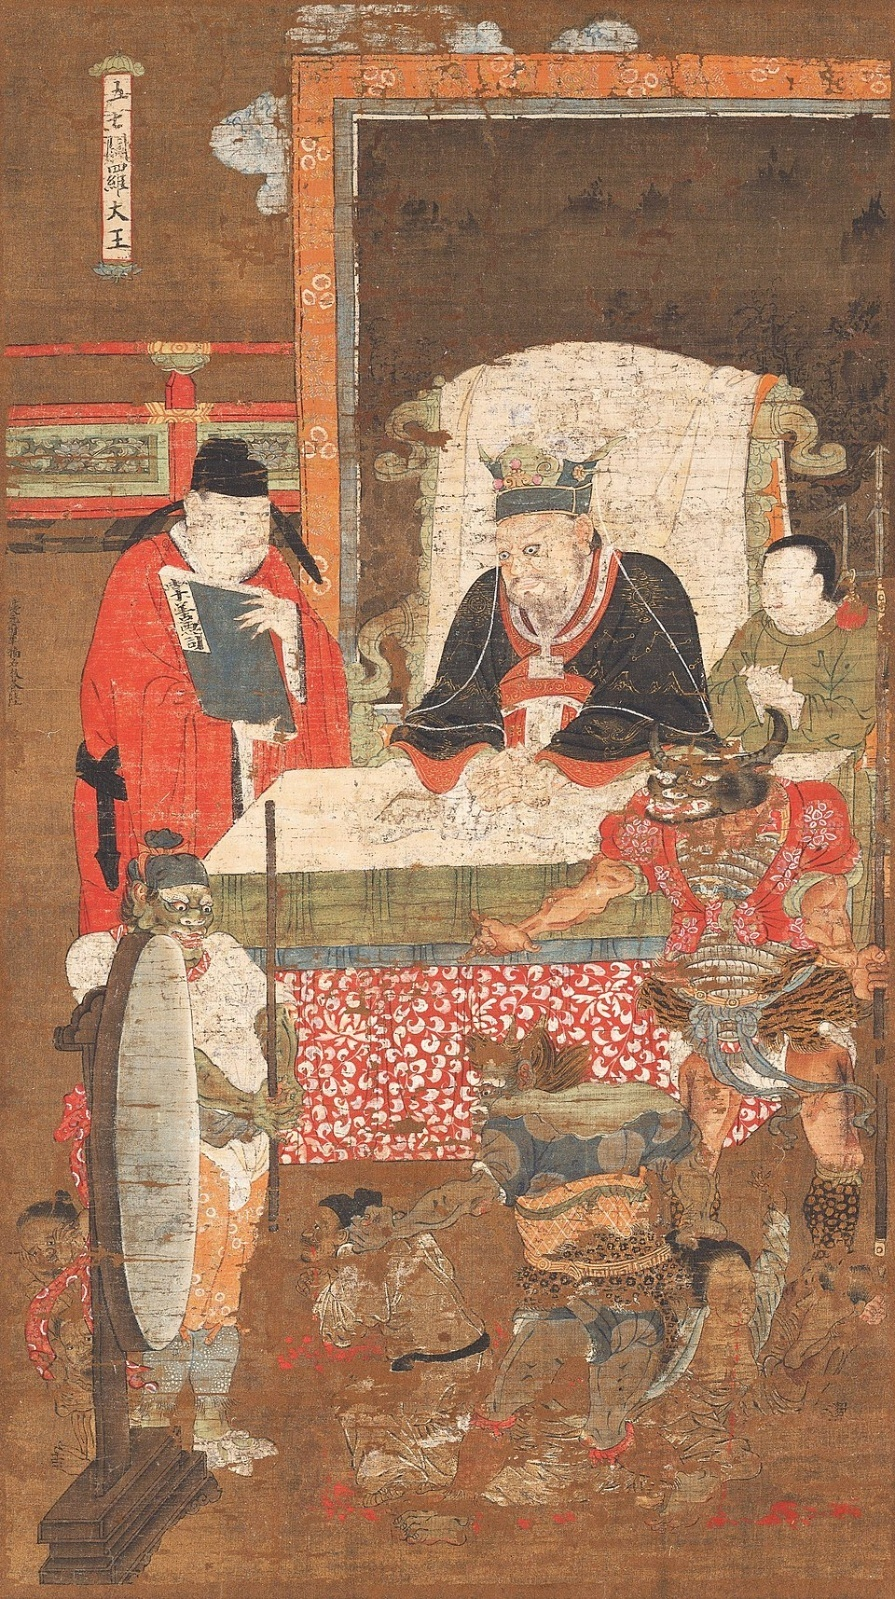
\includegraphics[width=0.85\linewidth,height=0.75\textheight,keepaspectratio]{image10.jpeg}
  \caption{Yanluo Wang, juiz dos mortos, em pintura da série \emph{Dez Reis do Inferno}, atribuída a Lu Xinzhong, século XIII.}
  \label{fig:cap2-img4}
\end{figure}

Esta pintura em seda é parte da série “Dez Reis do Inferno” e mostra Yanluo Wang (Enra Ō em japonês), juiz soberano dos mortos na tradição chinesa. A obra é atribuída a Lu Xinzhong e data da dinastia Song do Sul (século XIII), medindo 83,2 cm × 47,5 cm. O retrato representa o rei sentado em seu tribunal, ladeado por auxiliares, e integra um conjunto maior de pinturas que ilustram o julgamento das almas

No Japão, a tradição xintoísta concebia o Yomi, terra sombria dos mortos governada pela deusa Izanami, descrita no Kojiki (712 d.C.) como um local frio e impuro, semelhante em atmosfera à Irkalla mesopotâmica. Contudo, com a chegada do budismo (séc. VI d.C.), a cosmologia japonesa passou a adotar imagens de seis reinos de reencarnação, entre eles os infernos (Jigoku), concebidos como espaços de expiação temporária, onde as almas sofriam de acordo com seus pecados antes de renascerem.

A difusão do budismo na Ásia Oriental introduziu, assim, um modelo cíclico e corretivo de pós-morte, diferente da condenação eterna. Os inúmeros “infernos” descritos em sutras budistas (como o Sutra de K\d{s}itigarbha) não eram eternos, mas funcionavam como instâncias pedagógicas de sofrimento, das quais a alma eventualmente se libertava. Essa concepção influenciou tanto a iconografia chinesa e japonesa quanto a prática religiosa cotidiana, com rituais voltados para o alívio do sofrimento dos mortos.

Em síntese, o Extremo Oriente apresenta três camadas escatológicas principais:

O culto aos ancestrais (permanência comunitária e integração com os vivos);

A cosmologia taoísta (tribunais infernais e purificação);

A escatologia budista (infernos temporários e reencarnação).

Essas tradições fornecem uma visão de pós-morte menos centrada em dicotomias absolutas (salvação/danação) e mais orientada para a manutenção da ordem cósmica e social ou para o processo de purificação e renascimento.

\begin{longtable}{@{}p{2.2cm}p{3.2cm}p{2.5cm}p{3.2cm}p{3.7cm}@{}}
\caption{Comparação das concepções de além nas civilizações antigas.}\\
\toprule
\textbf{Tradição} & \textbf{Localização e governo} & \textbf{Critério} & \textbf{Condição pós-morte} & \textbf{Ênfase ritual e cultural} \\
\midrule
\endfirsthead
\toprule
\textbf{Tradição} & \textbf{Localização e governo} & \textbf{Critério} & \textbf{Condição pós-morte} & \textbf{Ênfase ritual e cultural} \\
\midrule
\endhead
Mesopotâmia & Irkalla, governada por Ereshkigal & Destino universal, sem distinção moral & Existência diminuída e comum a justos e ímpios & Ritos funerários e oferendas aos ancestrais \\
Egito & Duat, sob o julgamento de Osíris & Pesagem moral do coração & Campo de Juncos ou segunda morte por Ammit & Purificação, fórmulas funerárias e ética pessoal \\
Vale do Indo & Além sem nome textual preservado & Pureza e ritos funerários & Continuidade da vida condicionada por purificação e oferendas & Banhos rituais e sepultamentos com objetos \\
China e Japão & Reinos ancestrais, Yomi, Jigoku e tribunais de Yanluo Wang & Varia conforme a tradição & Integração ancestral, purificação ou renascimento & Culto aos ancestrais, transferência de mérito e ritos taoístas \\
\bottomrule
\end{longtable}

O panorama das concepções de submundo nas civilizações antigas revela tanto divergências radicais quanto constantes universais. A Mesopotâmia projetou uma visão de morte igualitária e inexorável, na qual todos os homens, independentemente de seus méritos, encontravam-se reduzidos à condição de sombra. O Egito, em contraste, transformou a morte em tribunal ético, onde a vida terrena era pesada contra a ordem cósmica de Maat, inaugurando uma concepção de julgamento moral que ecoaria em tradições posteriores. O Vale do Indo, embora mais enigmático, enfatizou a purificação ritual e a continuidade da ordem social no além, estabelecendo uma ponte conceitual para o desenvolvimento védico e hindu. Já o Extremo Oriente privilegiou a integração do morto à comunidade dos ancestrais ou sua purificação em tribunais e ciclos de renascimento, oferecendo uma visão mais dinâmica e processual da existência pós-morte.

Em conjunto, essas tradições demonstram que, desde os primórdios da história, o ser humano buscou no além não apenas respostas sobre o destino individual, mas também formas de legitimar a ordem terrena. A escatologia antiga funcionava como espelho das preocupações sociais: a Mesopotâmia refletia o peso do destino inescapável; o Egito, a centralidade da justiça e da ordem; o Indo, a purificação coletiva; e o Extremo Oriente, a perpetuação da linhagem e o equilíbrio cósmico.

Assim, o estudo comparativo dessas concepções evidencia que a ideia de submundo não é apenas uma especulação religiosa, mas também um instrumento de organização cultural, moldando práticas rituais, normas sociais e valores éticos. Ao observarmos essas tradições lado a lado, vemos emergir não apenas diferentes mapas do além, mas sobretudo o traço comum da humanidade: a necessidade de conferir sentido à morte e de projetar na eternidade as preocupações e esperanças da vida.


% --- Capítulo 3: O Hades e o Tártaro Greco-Romano ---
\chapter[Hades e Tártaro]{O Hades e o Tártaro Greco-Romano}
\index{Hades}
\epigraph{A concepção greco-romana do submundo evolui de um Hades homérico sombrio até a geografia moral complexa de Virgílio e dos filósofos tardios --- os círculos, regiões e juízes que viriam a moldar profundamente a imaginação cristã do além.}

A concepção greco-romana do submundo representa um desenvolvimento fascinante na evolução das ideias sobre o além. Enquanto as civilizações mesopotâmica e egípcia estabeleceram os fundamentos das noções de um mundo subterrâneo e julgamento póstumo, foram os gregos e, posteriormente, os romanos que desenvolveram uma geografia do além de incomparável riqueza e complexidade, com regiões distintas que refletiam diferentes destinos morais.

Esta sofisticação não surgiu de repente, mas evoluiu ao longo de séculos, desde as concepções homéricas relativamente simples de um Hades sombrio até as descrições elaboradas de Virgílio e os filósofos tardios, que estabeleceram uma topografia moral complexa que influenciaria profundamente a ideia cristã do inferno. Neste capítulo, exploraremos a evolução das concepções greco-romanas do submundo, sua relação com as tradições anteriores e seu impacto duradouro no imaginário ocidental sobre o além.


\begin{figure}[ht]
  \centering
  \includegraphics[width=0.85\linewidth]{image11.png}
  \caption{A Geografia do Hades e seus Rios}
  \label{fig:cap3-img1}
\end{figure}

\section{A Geografia do Hades e seus Rios}

\subsection{A Evolução da Topografia Subterrânea}

Na tradição grega, o submundo -- geralmente denominado "Hades", tanto em referência ao local quanto à divindade que o governava -- não permaneceu um conceito estático, mas evoluiu significativamente desde Homero até o período helenístico tardio. Inicialmente, nas obras homéricas (séculos VIII-VII a.C.), o Hades era concebido como um reino sombrio e nebuloso, localizado sob a terra ou além do oceano, um destino universal para as sombras desprovidas de substância dos mortos.

A Odisseia de Homero apresenta uma das primeiras descrições detalhadas da topografia do submundo na literatura ocidental, quando Odisseu visita a "terra dos mortos" no Canto XI:

"Quando chegamos aos confins do profundo Oceano,
Lá fica o país e a cidade dos Cimérios, envolvidos em névoa e nuvens.
O sol brilhante nunca lança seus raios sobre eles,
Nem quando sobe ao céu estrelado nem quando desce da altura celeste;
Mas uma noite funesta paira sobre os infelizes mortais."

Gradualmente, nos períodos arcaico e clássico (c. 700-323 a.C.), esta visão relativamente indiferenciada cedeu lugar a uma geografia mais elaborada com divisões específicas. Na Teogonia de Hesíodo (c. 700 a.C.), já encontramos referências ao Tártaro como uma região distinta e particularmente sombria do submundo. Os poetas órficos e pitagóricos, por sua vez, desenvolveram ainda mais estas distinções, introduzindo a noção de diferentes destinos para diferentes tipos de almas.

\subsection{Os Rios do Submundo}

Um dos elementos mais distintivos e duradouros da topografia do Hades é o sistema de rios subterrâneos, que demarcam diferentes regiões e simbolizam diferentes aspectos da morte e do além. Cinco rios principais são comumente mencionados nas fontes clássicas, cada um com seu significado simbólico:

\begin{table}[ht]
  \centering
  \small
  \renewcommand{\arraystretch}{1.3}
  \caption{Os cinco rios do submundo grego e seus significados simbólicos.}
  \label{tab:rios-hades}
  \begin{tabularx}{\textwidth}{|>{\raggedright\arraybackslash}p{2.6cm}|>{\raggedright\arraybackslash}p{2.4cm}|>{\raggedright\arraybackslash}p{2.8cm}|X|}
    \hline
    \textbf{Rio} & \textbf{Significado etimológico} & \textbf{Características e simbolismo} & \textbf{Fontes e tradição} \\
    \hline
    Aqueronte & ``Rio da Dor'' & Primeiro rio encontrado pelas almas; atravessado com a ajuda do barqueiro Caronte; representa a transição para o estado de morte. & Hesíodo (filho da Terra e Tétis); mencionado na Odisseia e na Eneida. \\
    \hline
    Cócito & ``Rio do Lamento'' & Afluente do Aqueronte; seus sons evocam os lamentos dos mortos recentes; águas geladas que fluem para o Tártaro. & Platão, \emph{Fédon}. \\
    \hline
    Estige & ``Rio do Ódio'' & O mais sagrado dos rios infernais; por suas águas os deuses faziam juramentos invioláveis; águas venenosas que, em algumas tradições, conferiam invulnerabilidade (Aquiles). & Hesíodo (Teogonia); múltiplas fontes clássicas. \\
    \hline
    Lete & ``Rio do Esquecimento'' & Suas águas apagavam as memórias da vida anterior, preparando as almas para uma possível reencarnação. & Tradições órficas e platônicas. \\
    \hline
    Flegetonte & ``Rio de Fogo'' & Curso de água flamejante que circundava o Tártaro; rio de lava que ``ferve violentamente''. & Platão (Fédon); Virgílio (torrente de ``chamas crepitantes''). \\
    \hline
  \end{tabularx}
\end{table}


\begin{figure}[ht]
  \centering
  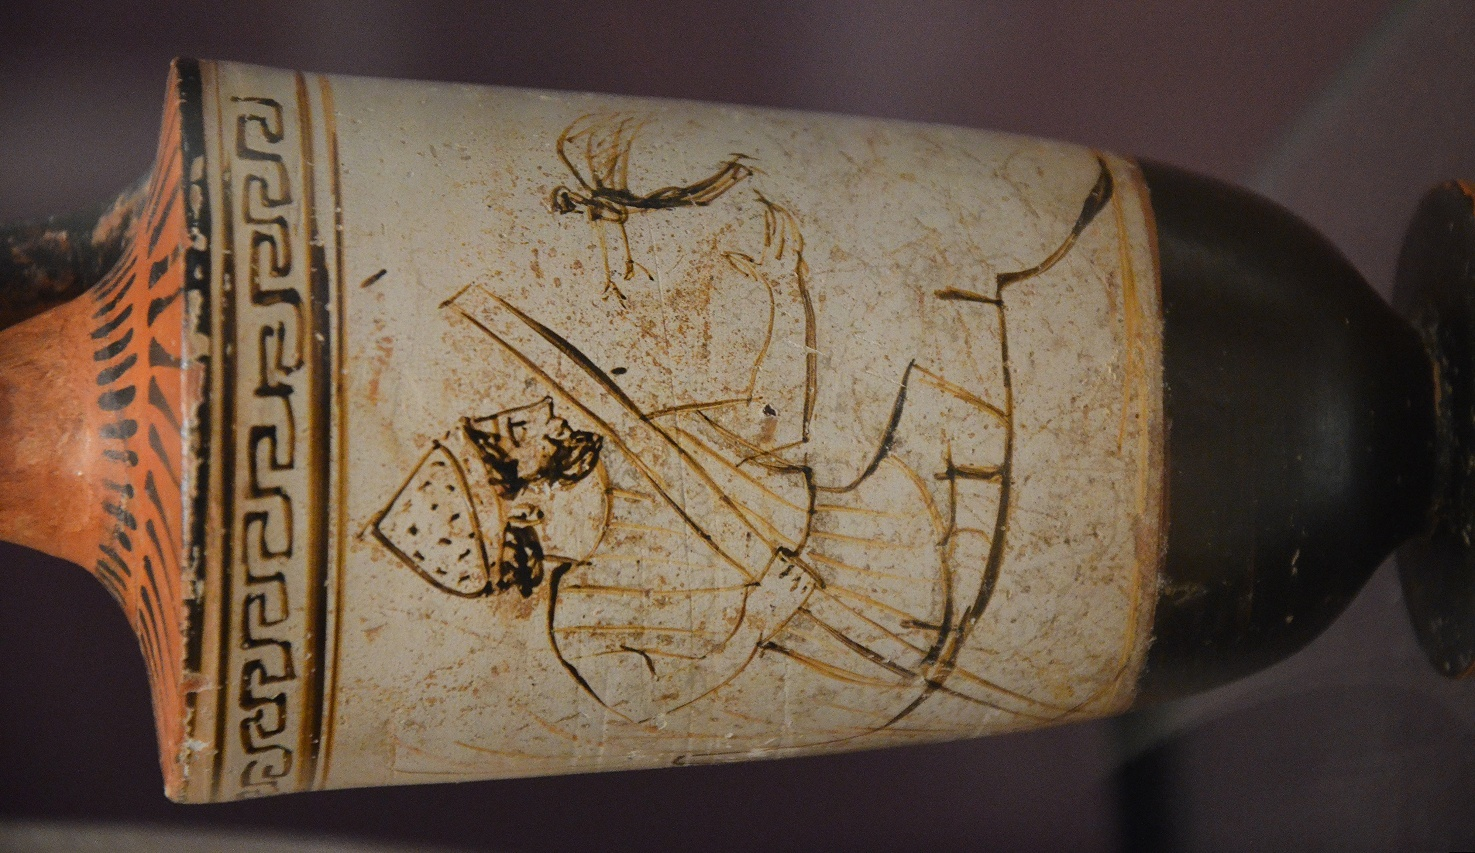
\includegraphics[width=0.85\linewidth]{image12.jpeg}
  \caption{Do Érebo aos Campos Elísios: As Regiões do Além}
  \label{fig:cap3-img2}
\end{figure}

Caronte transportando uma alma pelo rio Aqueronte. Lécito de fundo branco, c. 450 a.C. (Museu Ashmolean, Oxford). A figura do barqueiro permaneceria um elemento central na iconografia do inferno através dos séculos.

\section{Do Érebo aos Campos Elísios: As Regiões do Além}

Com o desenvolvimento da literatura e da filosofia gregas, o submundo gradualmente se diferenciou em regiões específicas, cada uma destinada a diferentes categorias de mortos. Esta topografia moral refletia valores sociais e preocupações éticas em evolução:

\begin{table}[ht]
  \centering
  \small
  \renewcommand{\arraystretch}{1.3}
  \caption{As quatro regiões do Hades grego e seus destinatários.}
  \label{tab:regioes-hades}
  \begin{tabularx}{\textwidth}{|>{\raggedright\arraybackslash}p{2.8cm}|>{\raggedright\arraybackslash}p{2.6cm}|>{\raggedright\arraybackslash}p{2.8cm}|X|}
    \hline
    \textbf{Região} & \textbf{Posição} & \textbf{Destinatários} & \textbf{Características} \\
    \hline
    Érebo & Antecâmara ou região limítrofe & Almas recém-chegadas, antes do julgamento & Limiar do Hades; local de espera antes da admissão no submundo. \\
    \hline
    Campos de Asfódelos & Região intermediária (maior parte do Hades) & Almas comuns --- nem virtuosas nem perversas & Planície monótona coberta de asfódelos (lírios); almas vagam como ``sombras sem vigor'' (Homero). \\
    \hline
    Campos Elísios (Ilhas dos Bem-Aventurados) & Paraíso grego & Inicialmente heróis favorecidos pelos deuses; mais tarde, justos e virtuosos & ``Onde a vida é mais fácil para os homens'': sem neve, sem inverno rigoroso, sem tempestades (Hesíodo). \\
    \hline
    Tártaro & Região mais profunda e sombria & Inicialmente Titãs derrotados; posteriormente, grandes criminosos e ímpios & Prisão primordial dos Titãs; local de punição dos grandes transgressores. Hesíodo: ``uma bigorna de bronze levaria nove dias e noites para cair do céu à terra, e mais nove para cair da terra ao Tártaro''. \\
    \hline
  \end{tabularx}
\end{table}


\begin{figure}[ht]
  \centering
  \includegraphics[width=0.85\linewidth]{image13.png}
  \caption{Campos de Asfódelos pelo olhar do Gemini.}
  \label{fig:cap3-img3}
\end{figure}

Campos de Afosdelos pelo olhar do Gemini.

\section{O Tártaro como Prisão dos Condenados}

\subsection{Origens do Tártaro na Mitologia Grega}

O Tártaro ocupa um lugar único na cosmologia grega. Nas fontes mais antigas, como a Ilíada de Homero, é mencionado como um abismo tão profundo quanto o céu é alto, localizado abaixo do próprio Hades. Na Teogonia de Hesíodo, desempenha um papel cosmológico crucial como prisão primordial dos Titãs após sua derrota na Titanomaquia:

"Ali os deuses Titãs estão ocultos sob a névoa sombria,
Por desígnio de Zeus ajuntador de nuvens,
Em um lugar bolorento, nos limites da vasta terra.
Não têm saída: Posêidon instalou portões de bronze,
E um muro corre em todas as direções ao seu redor."

\subsection{De Prisão Divina a Local de Punição Humana}

A transformação do Tártaro de uma prisão para divindades rebeldes em um local de punição para humanos ímpios ocorreu gradualmente, refletindo a crescente preocupação com justiça retributiva na cultura grega. Um marco importante nesta evolução é encontrado nas obras de Platão, particularmente no Górgias e no Fédon, onde ele desenvolve a ideia de punições pós-morte proporcionais às faltas cometidas em vida:

"Aqueles que são julgados incuráveis devido à magnitude de seus crimes -- sacrilégios múltiplos e graves, assassinatos injustos e ilegais, e outros males deste tipo -- são lançados no Tártaro, de onde nunca mais emergem." (Platão, Fédon)


\begin{figure}[ht]
  \centering
  \includegraphics[width=0.85\linewidth]{image14.jpeg}
  \caption{Os Castigos Eternos de Sísifo, Tântalo e Outros}
  \label{fig:cap3-img4}
\end{figure}

Cena do submundo grego em cratera de figuras vermelhas (c. 380 a.C.). A imagem mostra várias figuras míticas associadas ao Hades, incluindo o palácio do submundo. A crescente complexidade das representações visuais do além acompanhava a evolução das concepções literárias e filosóficas.

\section{Os Castigos Eternos de Sísifo, Tântalo e Outros}

\subsection{Os Grandes Condenados da Mitologia}

Entre os elementos mais memoráveis e influentes das concepções greco-romanas do submundo estão as histórias dos famosos condenados a castigos eternos no Tártaro. Estas figuras míticas, geralmente reis ou semideuses que desafiaram os deuses ou violaram tabus fundamentais, serviam como poderosos exemplos mitológicos de hybris (orgulho desmedido) e suas consequências.

Sísifo, antigo rei de Corinto, conhecido por sua astúcia e por enganar a própria Morte (Tânatos), foi condenado a empurrar eternamente uma pedra gigante montanha acima, apenas para vê-la rolar de volta quando chegava ao topo. Homero descreve seu tormento na Odisseia:

"Vi então Sísifo sofrendo duros trabalhos, empurrando com ambas as mãos uma pedra monstruosa. Esforçando-se com as mãos e os pés, ele empurrava a pedra montanha acima, mas quando estava prestes a transpor o cume, o peso fazia-o recuar, e a impiedosa pedra rolava novamente para a planície. Ele se esforçava novamente para empurrá-la para cima, seus membros suavam, e poeira levantava-se sobre sua cabeça."


\begin{figure}[ht]
  \centering
  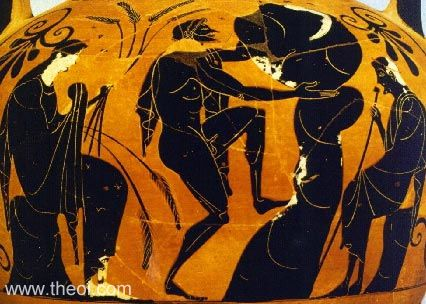
\includegraphics[width=0.85\linewidth]{image15.jpeg}
  \caption{Sísifo reinterpretado pelo Midjourney}
  \label{fig:cap3-img5}
\end{figure}

Sísifo empurrando sua pedra sob a supervisão de uma Fúria. Vaso grego de figuras vermelhas, c. 450 a.C. A punição de Sísifo tornou-se uma das mais emblemáticas representações do castigo eterno no imaginário ocidental.


\begin{figure}[ht]
  \centering
  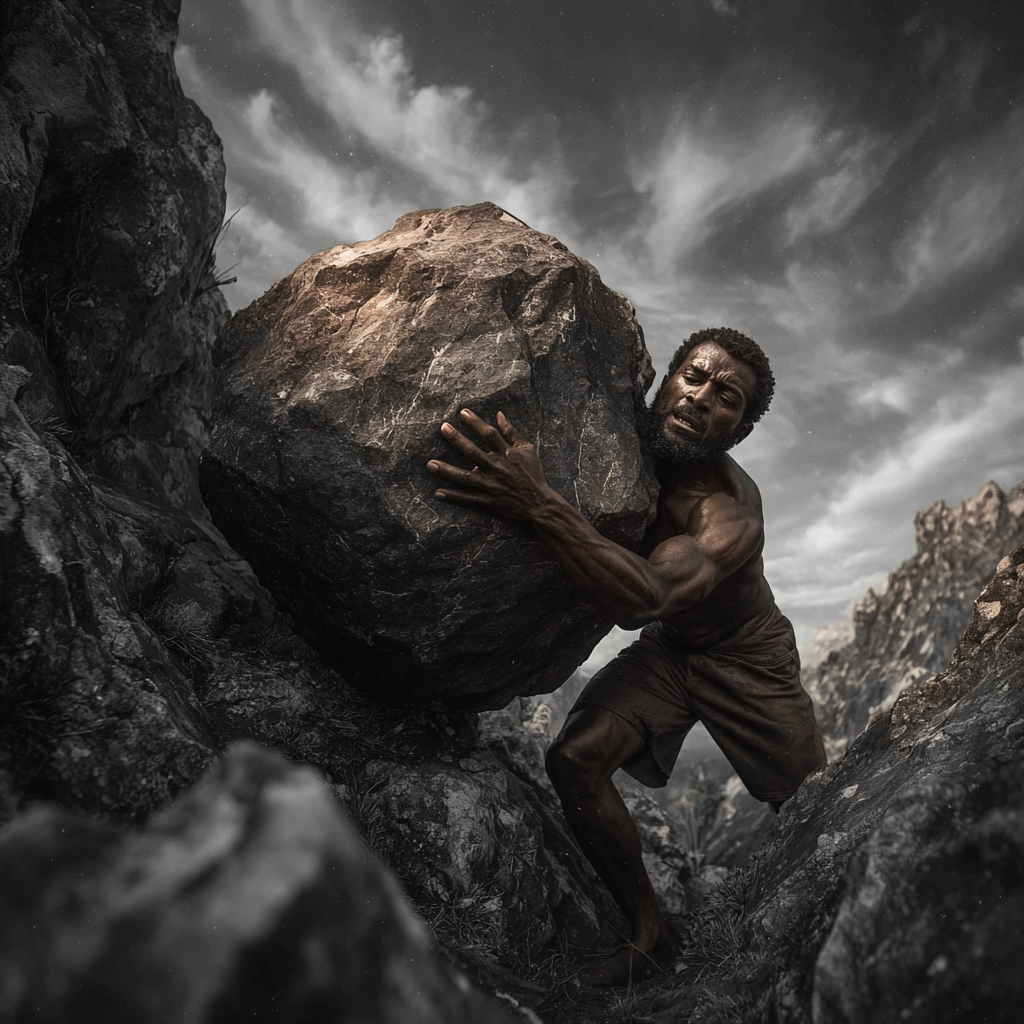
\includegraphics[width=0.85\linewidth]{image16.png}
  \caption{Sísifo reinterpretado pelo Midjourney}
  \label{fig:cap3-img6}
\end{figure}

Outros condenados famosos incluíam:

Tântalo, rei da Lídia e filho de Zeus, que ousou servir seu próprio filho como refeição aos deuses para testar sua onisciência, sofria de fome e sede eternas, apesar de estar posicionado com água até o queixo e frutos pendendo sobre sua cabeça -- ambos recuando sempre que tentava alcançá-los.

Ixíon, rei dos Lápitas, que tentou seduzir Hera e depois se gabou disso, foi amarrado a uma roda de fogo que girava eternamente.

As Danaides, cinquenta filhas de Dânao que assassinaram seus maridos na noite de núpcias (exceto uma), foram condenadas a encher eternamente jarros com fundos furados, numa tarefa infinita e fútil.


\begin{figure}[ht]
  \centering
  \includegraphics[width=0.85\linewidth]{image17.png}
  \caption{A Função Pedagógica e Moralística dos Castigos Exemplares}
  \label{fig:cap3-img7}
\end{figure}

\section{A Função Pedagógica e Moralística dos Castigos Exemplares}

Estas punições eternas não eram arbitrárias, mas invariavelmente refletiam a natureza das transgressões -- um princípio que seria mais tarde incorporado na concepção de contrapasso (contra passagem) na visão dantesca do inferno. Sísifo, que usou sua astúcia para enganar os deuses, está condenado a um trabalho inteligentemente inútil; Tântalo, que abusou da hospitalidade divina com uma refeição perversa, sofre eternamente de fome e sede; as Danaides, que destruíram suas uniões matrimoniais, estão presas a uma tarefa doméstica interminável.

\section{A Influência de Homero, Virgílio e Platão na Concepção do Além}

\subsection{Virgílio e a Consolidação da Topografia Infernal}

A descrição do submundo no Livro VI da Eneida de Virgílio representa a síntese mais completa e influente das concepções greco-romanas do além. Combinando elementos da tradição homérica, platônica, órfica e etrusca, Virgílio cria uma topografia infernal detalhada que serviria como modelo direto para Dante e outros autores medievais.

A jornada de Eneias pelo submundo, guiado pela Sibila, apresenta uma geografia claramente dividida em regiões morais. Após cruzar o Aqueronte com Caronte, Eneias passa pelos Campos do Luto (reservados para crianças, suicidas e vítimas de amor não correspondido), encontra o Tártaro (onde são punidos os criminosos) e finalmente chega aos Campos Elísios (morada dos heróis e virtuosos).

"Aqui Radamanto de Cnossos administra seu reino implacável,
Castiga, ouve confissões de engano -- quaisquer crimes
Que alguém, regozijando-se em fraude vã, tenha guardado
Secretamente em vida, adiando a expiação até tarde demais, até a morte."


\begin{figure}[ht]
  \centering
  \includegraphics[width=0.85\linewidth]{image18.jpeg}
  \caption{Mistérios Órficos e Eleusinos: Julgamento Moral, Metempsicose e Salvação Esotérica}
  \label{fig:cap3-img8}
\end{figure}

\section{Mistérios Órficos e Eleusinos: Julgamento Moral, Metempsicose e Salvação Esotérica}

A influência dos cultos de mistério grecoitalianos na construção de um além moralizado foi profunda e multifacetada. Os mistérios órficos, surgidos por volta do século VI a.C., introduziram no imaginário grego a ideia de que a alma, originariamente divina, estava aprisionada no corpo por culpa primitiva (o “pecado” dos Titãs) e deveria passar por um processo individual de purificação. Essa visão se materializou nas lâminas douradas órficas, laminelas de ouro enterradas com os iniciados entre a Magna Grécia e a Crimeia. As inscrições dessas lâminas descrevem um itinerário preciso após a morte: orientam o defunto a evitar o rio do esquecimento (Lethe) e a buscar a fonte da Memória (Mnemosyne), pois apenas a água da memória garante a identidade da alma. O morto é instruído a apresentarse aos guardiões infernais com fórmulas de reconhecimento como “sou filho da Terra e do Céu estrelado” e a implorar, “estou sedento, mas me dê logo água fria da Lagoa da Memória”. Outras lâminas mandam que se anuncie a Persefone que o Báquico (Dioniso) libertou a alma.

Além dessas “senhas” pósmortem, os órficos ensinavam que a alma deveria atravessar ciclos de reencarnação purificadora. De acordo com a tradição mítica, a humanidade nasceu das cinzas dos Titãs que devoraram Dioniso, motivo pelo qual cada alma contém um elemento dionisíaco aprisionado em corpo titânico. O pecador original obriga a alma a sofrer dez reencarnações para expiar os crimes dos Titãs. Somente a participação nos ritos órficos permitia reduzir esse ciclo: textos órficos enfatizam a doutrina da metempsicose, explicando que o iniciado deve evitar violência, praticar ascese e seguir as proibições alimentares para libertarse em três vidas. Aqueles que não passam pelos ritos permanecem “na lama e em doloroso servilismo” entre uma vida e outra, enquanto os iniciados aguardam a reencarnação “na companhia de Orfeu e dos deuses”, até serem finalmente libertados do ciclo. As lamelas, portanto, combinam julgamento moral individual (com perguntas e respostas na entrada do Hades) e possibilidade de purificação, oferecendo ao adepto uma rota para escapar da punição eterna.

Paralelamente, os mistérios eleusinos, ligados ao culto de Deméter e Perséfone em Eleusis, desenvolveram uma escatologia baseada na iniciação. Ao contrário do caminho místico órfico, que detalhava viagens pósmortem, os mistérios eleusinos prometiam aos participantes uma sorte venturosa simplesmente por terem “contemplado” os rituais secretos. O próprio Hino Homérico a Deméter (c. séculos VIIVI a.C.) faz essa distinção: após narrar a fundação dos ritos, proclama que “feliz é entre os mortais aquele que viu estas coisas; mas quem não participou dos ritos jamais terá parte [nisso] depois de morto, permanecendo nos reinos sombrios e úmidos”. Ou seja, o iniciado (designado com o termo olbios, “feliz, bemaventurado”) recebe a promessa de um destino abençoado, enquanto o nãoiniciado será condenado à “região úmida e nevoenta” do Hades. O mesmo hino acrescenta que as deusas “decidem amar” determinado mortal e enviam a ele Ploutos (Riqueza personificada), sugerindo que a iniciação assegurava prosperidade também em vida.

A comparação entre órficos e eleusinos evidencia dois caminhos complementares para a salvação no mundo grego: os órficos ofereciam conhecimento esotérico e técnicas para a alma atravessar o submundo e romper o ciclo das reencarnações; os eleusinos, por sua vez, asseguravam que a participação em rituais dramáticos e agrícolas proporcionava bem-aventurança pósmorte e evitava a existência abjeta “na escuridão e na sujeira”. Esses sistemas de crença foram fundamentais para a evolução de uma escatologia moralizada no Mediterrâneo, antecipando a noção de que a vida terrena e os ritos de iniciação determinam o destino eterno da alma.


\begin{figure}[ht]
  \centering
  \includegraphics[width=0.85\linewidth]{image19.jpeg}
  \caption{A Crítica Epicurista (Lucrécio) aos Terrores do Submundo}
  \label{fig:cap3-img9}
\end{figure}

Este mármore mostra Deméter sentada em um rochedo com um polos (coroa), Perséfone em pé segurando a chave de um templo e o herói Triptólemo (representado apenas pelas pernas) recebendo sementes. O Museu Getty explica que o relevo está ligado aos Mistérios de Eleusis, festivais que ofereciam “boa colheita e a possibilidade de uma vida melhor após a morte” aos iniciados; a cena inclui ainda um adorador em escala menor. A imagem reforça o aspecto agrário e iniciático dos mistérios eleusinos.

\section{A Crítica Epicurista (Lucrécio) aos Terrores do Submundo}

Nem todos os pensadores antigos aceitavam as concepções tradicionais do submundo e suas punições. Os epicuristas, em particular, desenvolveram uma crítica sistemática dessas ideias, baseada em seu materialismo filosófico. Esta crítica encontra sua expressão mais eloquente no poema De Rerum Natura (Sobre a Natureza das Coisas) de Lucrécio, escrito no século I a.C.

Lucrécio, seguindo os ensinamentos de Epicuro, argumentava que a alma, como o corpo, é material -- composta de átomos extremamente sutis -- e se dissolve completamente na morte. Portanto, não pode existir nenhuma forma de consciência, prazer ou sofrimento após a morte:

"Quando não existirmos mais, quando houver ocorrido a separação do corpo e da alma, cuja união forma nossa essência, é certo que nada absolutamente poderá atingir-nos, nem despertar então nossos sentidos, nem mesmo que a terra se confunda com o mar e o mar com o céu."


\begin{figure}[ht]
  \centering
  \includegraphics[width=0.85\linewidth]{image20.jpeg}
  \caption{Desmitologização dos Castigos Infernais}
  \label{fig:cap3-img10}
\end{figure}

\subsection{Desmitologização dos Castigos Infernais}

Uma estratégia central de Lucrécio é reinterpretar alegoricamente as histórias dos famosos condenados ao Tártaro, sugerindo que representam não punições póstumas, mas sofrimentos psicológicos experimentados em vida:

"Tântalo, como dizem as lendas, paralisado de terror, teme uma enorme rocha que pende sobre ele no ar: isto é uma imagem da vida humana, onde o vão temor dos deuses oprime os mortais, e cada um receia os golpes que o acaso pode trazer."

"Sísifo está também diante de nossos olhos, querendo obter do povo os feixes e os machados cruéis, e sempre retirando-se vencido e aflito. Pois buscar poder, que é na realidade vazio e nunca alcançado, e sofrer por isso contínuo trabalho, isto é empurrar com grande esforço uma pedra morro acima, que logo depois rola de volta à planície."

Através desta técnica de desmitologização, Lucrécio efetivamente inverte a função moral tradicional dos mitos de punição eterna: em vez de serem avisos sobre consequências além-túmulo, tornam-se reflexos das consequências psicológicas imediatas de certos comportamentos e atitudes durante a vida.


\section{Síntese e Inovação}

A concepção greco-romana do submundo representa um desenvolvimento crucial na evolução das ideias sobre o além. Embora claramente influenciada por tradições anteriores do Oriente Próximo, a visão clássica do Hades e Tártaro introduziu inovações significativas:

Topografia moral elaborada: A divisão do além em regiões distintas correspondentes a diferentes categorias morais -- uma estruturação espacial da justiça cósmica.

Personalização dos castigos: A correspondência entre a natureza da transgressão e a forma específica de punição, estabelecendo um princípio de justiça poética no além.

Tensão filosófica-mitológica: A coexistência de interpretações literais, alegóricas e filosóficas do submundo, criando uma rica tradição interpretativa.

Democratização do além: A evolução de um destino inicialmente reservado para transgressores extraordinários (como os grandes condenados mitológicos) para um sistema universal de julgamento aplicável a todos.

\section{O Impacto na Tradição Ocidental}

A concepção greco-romana do submundo exerceu um impacto profundo e duradouro na cultura ocidental, tanto diretamente -- através da preservação e transmissão de textos clássicos -- quanto indiretamente, mediante sua absorção e transformação por tradições religiosas posteriores, particularmente o cristianismo.

O exemplo mais notável desta influência é encontrado na Divina Comédia de Dante, cuja estruturação do Inferno deve muito a Virgílio (não por acaso escolhido como guia do poeta). A disposição em círculos concêntricos, a correspondência entre pecado e castigo (contrapasso), e muitas imagens específicas derivam diretamente da tradição clássica.

Mesmo na era contemporânea, marcada por secularização e ceticismo quanto a concepções literais de punição além-túmulo, os elementos fundamentais do submundo greco-romano continuam a exercer influência cultural significativa, nas artes, na literatura, no cinema e em outras manifestações culturais.

Esta persistência atesta não apenas o poder imaginativo das concepções clássicas do submundo, mas também sua capacidade de expressar preocupações humanas perenes relacionadas a justiça, consequência moral e a relação entre ações em vida e destino final.

% ============================================================
%  PARTE II: TRADIÇÕES REGIONAIS E CULTURAIS
% ============================================================

\part{TRADIÇÕES REGIONAIS E CULTURAIS}
\partmark{TRADIÇÕES REGIONAIS E CULTURAIS}

% --- Capítulo 5: Helheim - O Reino Gelado dos Mortos na Mitologia Nórdica ---
\chapter[Helheim (Nórdico)]{Helheim - O Reino Gelado dos Mortos na Mitologia Nórdica}
\index{Helheim}
\epigraph{A tradição nórdica apresenta uma das concepções mais singulares de submundo: um reino de gelo e imobilidade, menos suplício físico que aniquilação simbólica, reservado aos que não conquistaram a glória heroica.}

A tradição nórdica apresenta uma das concepções mais singulares de submundo na história das religiões, marcada por um imaginário radicalmente distinto dos modelos mediterrâneos. Enquanto o inferno greco-romano ou cristão enfatiza o fogo purificador e o tormento ativo, o Helheim escandinavo é concebido como um reino de gelo, escuridão e imobilidade, onde a ausência de calor e de vitalidade se converte na própria essência da punição. Trata-se menos de suplício físico e mais de aniquilação simbólica, um destino frio e sombrio reservado àqueles que não conquistaram a glória heroica.

As principais fontes textuais para esse imaginário encontram-se na Edda Prosaica de Snorri Sturluson (c. 1220) e na Edda Poética (compilada entre os séculos XIII-XIV a partir de tradições orais). Entre os poemas, destaca-se a Völuspá, que descreve Helheim como um dos nove mundos suspensos nas raízes de Yggdrasil, a árvore cósmica que sustenta o universo. Essa localização não marginaliza o reino dos mortos como punição divina, mas o integra na ordem cósmica -- Helheim existe porque o equilíbrio do universo exige um espaço para os que morrem de velhice ou doença, em contraposição aos guerreiros conduzidos a Valhalla ou Fólkvangr.

A figura de Hel, filha de Loki e da giganta Angrboda, simboliza essa ambivalência: metade de seu corpo é de carne viva, metade em estado de decomposição. Seu governo não é de maldade absoluta, mas de necessidade cósmica. Helheim é, portanto, menos inferno no sentido cristão do termo e mais um reino paralelo, que preserva o equilíbrio entre vida e morte. A própria Hel reflete a concepção germânica de que o mundo é sustentado pela tensão entre forças opostas, não pela exclusão moral de um lado sobre o outro.


\begin{figure}[ht]
  \centering
  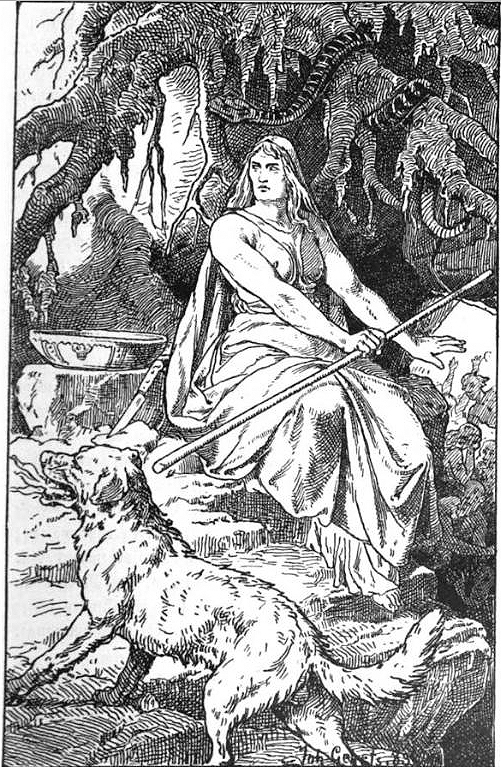
\includegraphics[width=0.85\linewidth]{image21.png}
  \caption{Hel (1889) por Johannes Gehrts – mostra a deusa Hel, metade viva, metade morta, com o cão Garmr aos seus pés, representando o caráter ambíguo e não-moralizante do seu reino.}
  \label{fig:cap5-img1}
\end{figure}

Hel (1889) por Johannes Gehrts -- mostra a deusa Hel, metade viva, metade morta, com o cão Garmr aos seus pés, representando o caráter ambíguo e não-moralizante do seu reino.


\begin{figure}[ht]
  \centering
  \includegraphics[width=0.85\linewidth]{image22.png}
  \caption{Móðguðr guardando a ponte Gjallarbrú (Louis Moe, 1929) – a guardiã impede a passagem até que a alma declare seu nome, simbolizando o limiar entre os vivos e Helheim.}
  \label{fig:cap5-img2}
\end{figure}

Móðguðr guardando a ponte Gjallarbrú (Louis Moe, 1929) -- a guardiã impede a passagem até que a alma declare seu nome, simbolizando o limiar entre os vivos e Helheim.

A geografia mítica de Helheim reforça esse caráter de alteridade. O rio Gjöll, guardado pela donzela Móðguðr, marca a fronteira entre vivos e mortos, atravessada pela ponte Gjallarbrú. O salão de Hel, Éljúdnir, possui teto de ossos de serpentes e piso de entranhas, sugerindo não o tormento ativo, mas um ambiente de decadência permanente e inescapável. O frio, a escuridão e o silêncio são descritos como mais letais do que o fogo -- uma negação da vida em sua essência.

No que tange à punição, a tradição nórdica se afasta de sistemas baseados em julgamento moral universal. A maioria dos mortos em Helheim experimenta uma existência neutra, sem recompensas ou tormentos desmedidos. O sofrimento mais profundo não é o castigo físico, mas a separação da comunidade guerreira, a exclusão da memória heroica e do canto dos escaldos. A vergonha de uma morte não-heroica representa, na ética germânica, uma condenação mais terrível que o suplício corporal.

Uma exceção é Náströnd (“Costa dos Cadáveres”), região afastada do sol, onde perjuros, assassinos e adúlteros sofrem punições explícitas: aprisionados em salões de espinhas de serpentes, são continuamente envenenados por répteis gotejantes. Aqui a tradição nórdica se aproxima de modelos mediterrâneos de inferno punitivo, mas aplica-os apenas a quem violou códigos sociais fundamentais. Para todos os demais, Helheim não é espaço de justiça moral, mas de destinação inevitável.


\begin{figure}[ht]
  \centering
  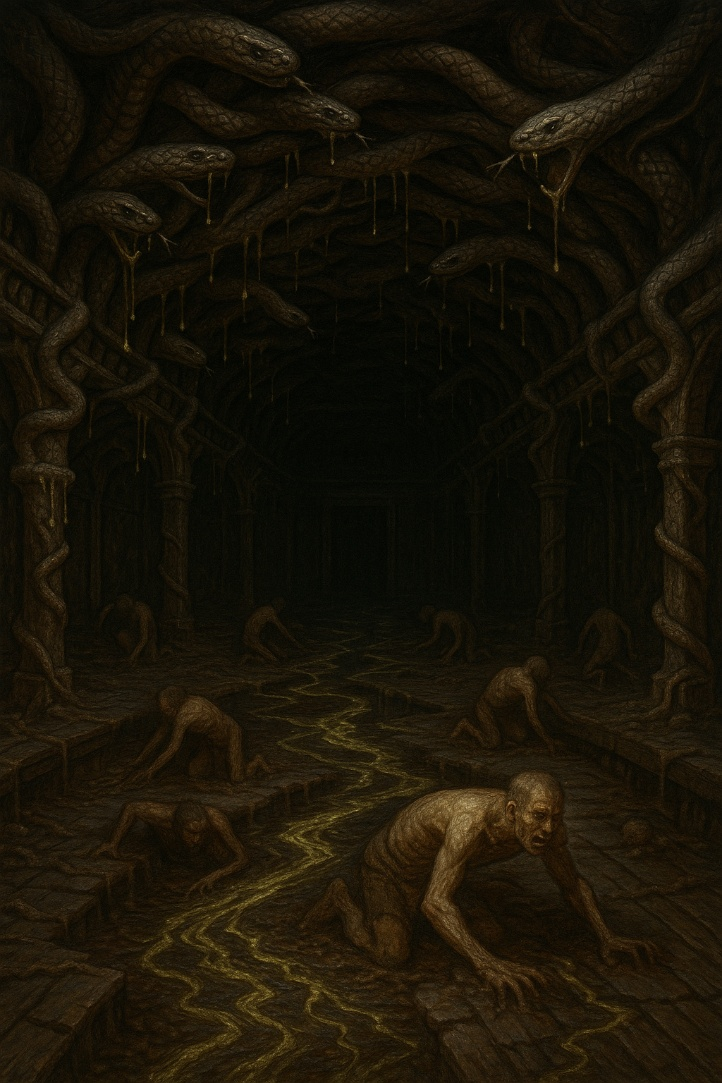
\includegraphics[width=0.85\linewidth]{image23.jpeg}
  \caption{Visão artística de Helheim como reino frio e sombrio destinado à maioria dos mortos na cosmologia nórdica.}
  \label{fig:cap5-img3}
\end{figure}

O Ragnarök, a batalha final, introduz uma dimensão escatológica própria: mesmo os mortos de Helheim terão papel no fim dos tempos. Conduzidos pelo navio Naglfar, feito de unhas humanas, eles emergirão para lutar contra os deuses. Essa visão contrasta com concepções de condenação estática: na mitologia nórdica, nem mesmo a morte é definitiva -- o cosmos é dinâmico e todos, vivos e mortos, participam de sua destruição e possível renovação.


\begin{figure}[ht]
  \centering
  \includegraphics[width=0.85\linewidth]{image24.jpeg}
  \caption{Naglfar, o navio dos mortos, navegando rumo à batalha final do Ragnarök; ilustração de Louis Moe, 1929.}
  \label{fig:cap5-img4}
\end{figure}

O navio Naglfar é descrito nas Eddas como a embarcação dos condenados, feita de unhas de pessoas mortas; na ilustração de Louis Moe (1929) ele navega rumo ao Ragnarök. O texto do MyNDIR explica que no Prosa Edda o timoneiro é Loki, mas em Völuspá é o gigante Hrymr, e que a cena pertence ao livro Ragnarok: En Billeddigtnin

Com a cristianização da Escandinávia (sécs. X-XII), elementos de Helheim foram reinterpretados. Textos como o Draumkvaede e o Sólarljóð mesclam paisagens gélidas do submundo nórdico com o esquema cristão de julgamento moral, criando um sincretismo fascinante. Ainda assim, a persistência de temas helheimicos em lendas e folclore escandinavos posteriores -- desde aparições fantasmagóricas até crenças em locais amaldiçoados -- demonstra a longevidade cultural dessa concepção singular de pós-morte.


% --- Capítulo 6: Xibalba, Mictlan e Supay - Mundos Subterrâneos das Américas Pré-Colombianas ---
\chapter[Xibalba, Mictlan, Supay]{Xibalba, Mictlan e Supay - Mundos Subterrâneos das Américas Pré-Colombianas}
\index{Xibalba}\index{Mictlan}\index{Supay}


\epigraph{As civilizações pré-colombianas desenvolveram concepções sofisticadas de mundos subterrâneos que rivalizam em complexidade com tradições do Velho Mundo, oferecendo perspectivas únicas sobre punição eterna, julgamento moral e geografia espiritual. Estas tradições, preservadas em códices, monumentos arqueológicos e tradições orais, revelam sistemas cosmológicos integrados onde os submundos constituem componentes essenciais da ordem universal.}

Xibalba, o submundo maia conforme descrito no Popol Vuh (manuscrito k'iche' do séc. XVI baseado em tradições orais antigas), representa uma das mais detalhadas geografias infernais nas Américas. Governado pelos Senhores da Morte, particularmente Hun-Camé ("Um-Morte") e Vucub-Camé ("Sete-Morte"), Xibalba constitui reino de provas e transformações onde almas enfrentam desafios elaborados que determinam seu destino final. A descida dos heróis gêmeos Hunahpú e Ixbalanqué oferece paradigma para navegação pós-morte através de rituais específicos e conhecimento esotérico.


\begin{figure}[ht]
  \centering
  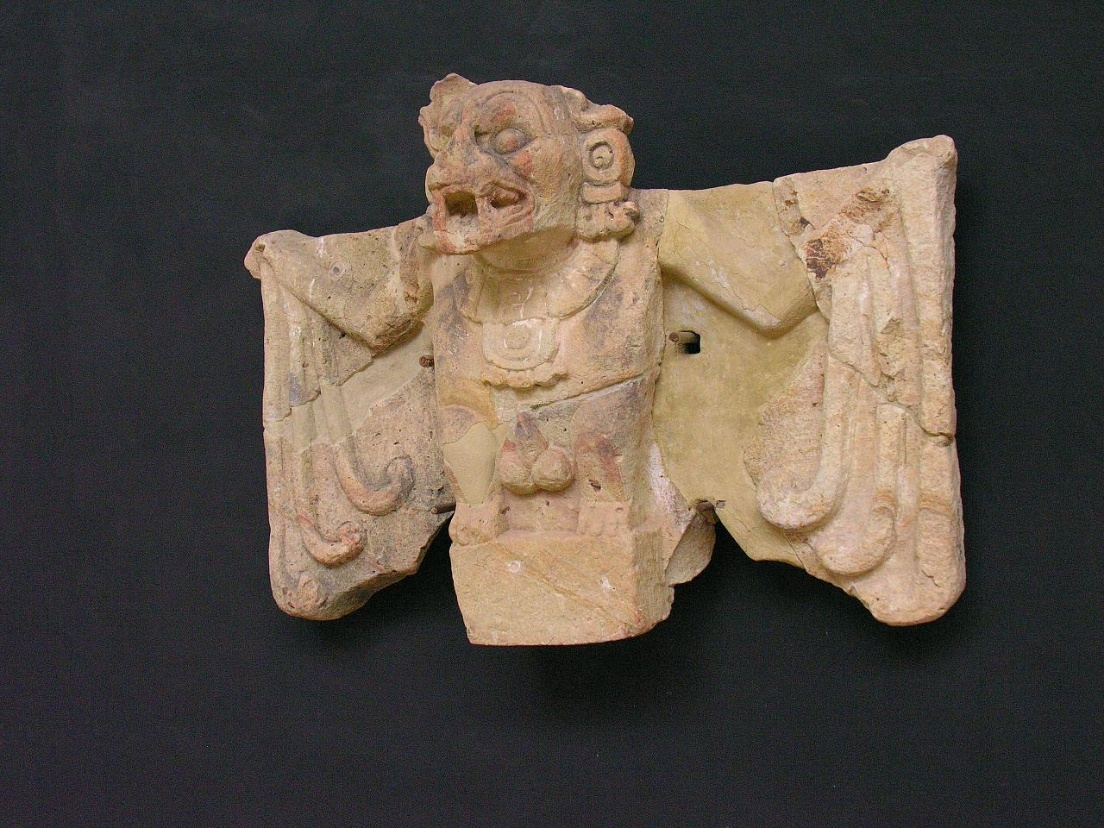
\includegraphics[width=0.85\linewidth]{image25.jpeg}
  \caption{Escultura de Camazotz proveniente de Copán, Honduras; o morcego é associado aos Senhores de Xibalba e aos domínios da noite e da morte.}
  \label{fig:cap6-img1}
\end{figure}

Foto de uma escultura em forma de morcego (Camazotz), proveniente de Copán, Honduras. O morcego (“Killer Bat”) é associado aos Senhores de Xibalba e aos domínios da noite e da morte

A estrutura de Xibalba inclui múltiplas casas de tormento, cada uma representando diferentes aspectos da experiência mortal levados ao extremo. A Casa das Trevas (submersão em escuridão absoluta), Casa das Facas (lâminas cortantes infinitas), Casa do Frio (frieza extrema), Casa dos Jaguares (predadores ferozes), Casa do Fogo (calor consumidor), e Casa dos Morcegos (Camazotz, o deus-morcego decapitador) criam sequência de provas que testam coragem, inteligência e preparação ritual dos mortos.

Mictlan, o submundo asteca, oferece concepção geograficamente estratificada de nove níveis subterrâneos governados por Mictlantecuhtli ("Senhor dos Mortos") e sua consorte Mictlancihuatl ("Senhora dos Mortos"). Diferentemente de sistemas baseados em julgamento moral, Mictlan opera segundo princípios de tipo de morte e preparação ritual. Guerreiros mortos em combate ascendem ao paraíso oriental de Tonatiuhichan, mulheres mortas no parto transformam-se em Cihuateteo (mulheres divinas), enquanto a maioria empreende jornada de quatro anos através dos nove níveis de Mictlan.

A jornada através de Mictlan envolve série de obstáculos geográficos e espirituais que requerem preparação específica. O morto deve atravessar rios caudalosos com ajuda de cão psicopompo (xoloitzcuintli), superar montanhas que se chocam, resistir a ventos cortantes capazes de despir carne dos ossos, e enfrentar serpentes e lagartos

gigantescos. Esta jornada culmina na audiência com Mictlantecuhtli, onde o morto apresenta oferendas específicas (jade, incenso, tecidos) para garantir descanso final.


\begin{figure}[ht]
  \centering
  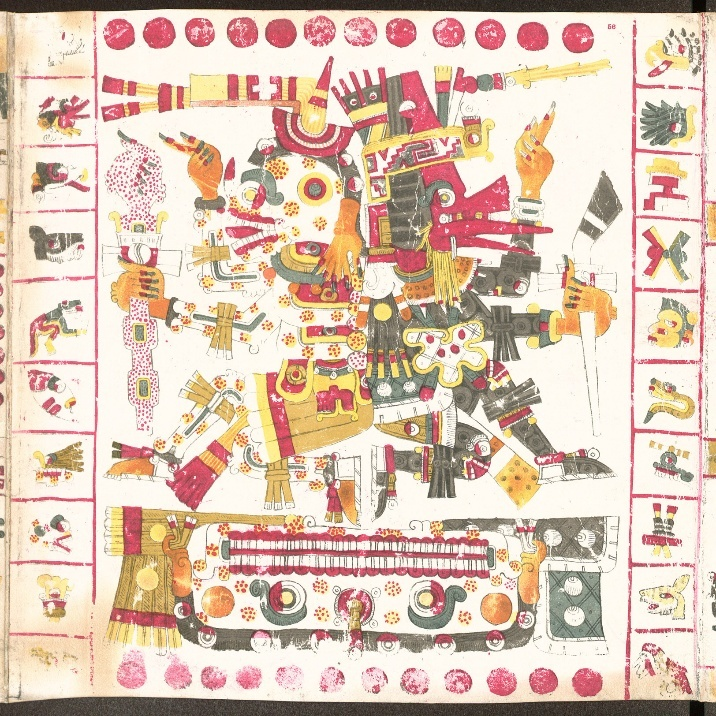
\includegraphics[width=0.85\linewidth]{image26.jpeg}
  \caption{Mictlantecuhtli e Quetzalcóatl na página 56 do Códice Borgia, associados à morte e à renovação da vida.}
  \label{fig:cap6-img2}
\end{figure}

Página 56 do Códice Borgia: o deus da morte Mictlantecuhtli aparece à esquerda e Quetzalcóatl à direita; juntos representam a primeira morte e a segunda vidacommons.wikimedia.org. A obra é uma reprodução fidedigna do manuscrito pré-colombiano, em domínio público.

A concepção inca de Supay e o submundo andino reflete adaptação a geografia montanhosa única. Supay, frequentemente traduzido como "diabo" pelos missionários espanhóis, representa na verdade divindade ctônica complexa que governa tanto riquezas minerais quanto mortos. O submundo inca localiza-se nas profundezas terrestres, acessível através de cavernas e fontes naturais consideradas portais entre mundos. Esta geografia sagrada integra paisagem física andina com cosmologia espiritual, criando mapa sagrado where specific locations serve as interfaces entre worlds.

Os processos de colonização europeia e evangelização cristã nas Américas criaram sincretismos complexos entre tradições pré-colombianas e conceitos cristãos de inferno. A interpretação de Xibalba como "inferno cristão" pelos missionários facilitou preservação de elementos indígenas sob terminologia cristã. Documentos coloniais como os Anales de Cuauhtitlan e o Códice Florentino preservam descrições de submundos pré-colombianos filtradas através de conceitos cristãos, criando sínteses únicas.

A persistência de elementos pré-colombianos em tradições populares contemporâneas demonstra vitalidade cultural destas concepções. O Día de los Muertos mexicano preserva elementos de comunicação com mortos em Mictlan, enquanto tradições andinas mantêm oferendas a Supay para proteção em atividades mineiras. Estas continuidades culturais ilustram adaptabilidade de cosmologias indígenas face a pressões evangelizadoras europeias.


\section{Comparação entre Xibalba, Mictlan e Ukhu Pacha}

\begin{description}[leftmargin=2.8cm,style=nextline]
  \item[Xibalba] Governado por Hun-Camé e Vucub-Camé, os Senhores da Morte.
  Suas casas de tormento submetem os viajantes a provas de trevas, lâminas,
  frio, jaguares, fogo e morcegos.
  \item[Mictlan] Governado por Mictlantecuhtli e Mictlancihuatl. A travessia
  compreende nove níveis e exige que o morto supere sucessivos obstáculos.
  \item[Ukhu Pacha] Mundo inferior andino governado por Supay, divindade
  ctônica associada aos mortos e às riquezas minerais.
\end{description}

As casas de tormento de Xibalba incluem:

\begin{itemize}
  \item Trevas
  \item Facas
  \item Frio
  \item Jaguares
  \item Fogo
  \item Morcegos (Camazotz)
\end{itemize}
Os nove níveis da travessia de Mictlan incluem:

\begin{itemize}
  \item Rio com cão psicopompo
  \item Montanhas colidindo
  \item Ventos cortantes
  \item Serpentes
  \item Lagartos gigantes
  \item Obstáculos adicionais
\end{itemize}
O Ukhu Pacha é um submundo ligado a cavernas, minas e fontes naturais.

Em Xibalba, o acesso depende de provas rituais e conhecimento esotérico;
seu horizonte narrativo é a transcendência ou dissolução, representada
pelos heróis gêmeos Hunahpú e Ixbalanqué. Em Mictlan, o destino depende do
tipo de morte e da preparação ritual: após quatro anos de travessia e das
oferendas a Mictlantecuhtli, alcança-se o repouso. No mundo andino, o acesso
é universal e não moralista, ligado à integração com os ancestrais e com as
forças da terra.

A análise comparativa revela paralelos estruturais notáveis entre submundos americanos e tradições do Velho Mundo, sugerindo arquétipos recorrentes na organização de conceitos escatológicos. Todos apresentam geografia estratificada, provas rituais, divindades governantes duais (masculina/feminina) e ênfase em preparação adequada para a navegação pós-morte. Essas similaridades, desenvolvidas independentemente, sugerem constantes antropológicas na conceituação humana do destino pós-morte.


\begin{figure}[ht]
  \centering
  \includegraphics[width=0.85\linewidth]{image27.jpeg}
  \caption{Máscara boliviana de China Supay em gesso policromado, início do século XX, pertencente ao Musée du quai Branly.}
  \label{fig:cap6-img3}
\end{figure}

Máscara de China Supay, em gesso policromado, originária da Bolívia (início do século XX). A peça faz parte das coleções do Musée du quai Branly e representa o ser ctônico que preside o submundo andino e as riquezas minerais.


% --- Capítulo 7: Tradições Célticas e Germânicas ---
\chapter[Tradições Célticas]{Tradições Célticas e Germânicas}
\index{Annwn|see{Outro Mundo céltico}}\index{Outro Mundo céltico}\index{Sídhe}


\epigraph{As tradições célticas e germânicas pré-cristãs desenvolveram concepções distintivas de mundos subterrâneos e punição pós-morte que exerceram influência profunda na formação do cristianismo medieval europeu. Estas tradições, preservadas em literatura vernácula, folclore e evidências arqueológicas, revelam sistemas cosmológicos sofisticados que resistiram à cristianização através de processos de sincretismo e reinterpretação cultural.}

O conceito céltico de Annwn, o Outro Mundo subterrâneo descrito particularmente na literatura galesa medieval, representa um reino paralelo acessível através de lagos, colinas sagradas (sidhe) e outros portais naturais. O Mabinogi, coletânea de contos galeses dos sécs. XI-XIII baseados em tradições orais mais antigas, apresenta Annwn como reino governado por reis como Arawn e Gwyn ap Nudd, onde diferentes leis temporais e morais operam. Significativamente, Annwn não constitui local de punição, mas reino alternativo onde heróis podem obter objetos mágicos e conhecimento esotérico.

A literatura irlandesa preserva concepções similares através do conceito de Sídhe, tanto como locais físicos (montículos funerários neolíticos) quanto como dimensão espiritual habitada pelos Tuatha Dé Danann após sua retirada do mundo humano. O Táin Bó Cúailnge e outros ciclos épicos irlandeses descrevem interações frequentes entre mundos humano e sidhe, onde heróis como Cú Chulainn empreendem jornadas ao Outro Mundo para completar geas (obrigações místicas) ou obter armas sobrenaturais.

A tradição germânica continental, parcialmente preservada em textos como o Heliand saxão (séc. IX) e evidências arqueológicas de práticas funerárias, revela concepções de submundo relacionadas mas distintas das tradições nórdicas. O conceito de Hel germânico primitivo aparece associado não apenas à divindade feminina dos mortos, mas a estados de ocultação e transformação espiritual. Evidências arqueológicas de "boat burials" e oferendas mortuárias sugerem crenças em jornadas pós-morte através de reinos aquáticos subterrâneos.

Os processos de cristianização das Ilhas Britânicas (sécs. V-VIII) criaram sínteses únicas entre tradições célticas e conceitos cristãos de inferno. A conversão de reis como Æthelberht de Kent (c. 601) e Edwin da Nortúmbria (627) facilitou desenvolvimento de literatura cristã vernácula que preserva elementos païos significativos. O poema anglo- saxão Christ and Satan (séc. VIII-IX) apresenta descrições de inferno que incorporam elementos de paisagens nórdicas e germânicas, incluindo ênfase em frieza e desolação.

A influência druídica na formação de conceitos cristãos irlandeses representa fenômeno de particular importância. Textos como o Acallamh na Senórach (séc. XII) preservam tradições sobre druidas convertidos que mantêm conhecimento esotérico sobre navegação entre mundos. A figura de Merlim na literatura arturiana representa síntese de sabedoria druídica com elementos cristãos, criando arquétipo de sábio que compreende tanto Annwn quanto inferno cristão.

A literatura visionária irlandesa medieval, particularmente textos como Fís Adamnáin (Visão de Adamnán, séc. X-XI) e Aisling Óenguso (Sonho de Óengus), desenvolve geografias de Outro Mundo que integram elementos célticos tradicionais com cosmologia cristã. Estas visões apresentam paisagens que combinam sidhe tradicional com descrições de purgatório e inferno, criando sínteses geográficas únicas que influenciarão desenvolvimentos continentais posteriores.

O folclore céltico posterior preserva elementos pré-cristãos através de contos sobre "fairy hills", "ghost roads", e outros fenômenos liminais que conectam mundo dos vivos com reinos dos mortos. A persistência de tradições como Samhain (Halloween) demonstra continuidade cultural de conceitos sobre comunicação temporária entre mundos durante períodos específicos do calendário astronômico.

A análise linguística de terminologias célticas e germânicas para conceitos escatológicos revela stratificação cultural complexa. Termos irlandeses como tech duinn ("casa escura") e aos sí ("folk dos sidhe") preservam elementos de cosmologia pré-cristã, enquanto empréstimos latinos como peccad (pecado) e diabul (diabo) demonstram influência cristã. Esta coexistência terminológica reflete sincretismo conceitual profundo que caracteriza cristianismo céltico.


% --- Capítulo 8: Tradições Eslavas e Bizantinas ---
\chapter[Tradições Eslavas]{Tradições Eslavas e Bizantinas}
\index{Nav}


\epigraph{As tradições eslavas e bizantinas representam desenvolvimentos únicos na evolução dos conceitos infernais, combinando elementos de paganismo eslavo primitivo com sofisticadas elaborações teológicas orientais. Esta síntese, facilitada pela conversão do mundo eslavo ao cristianismo bizantino entre os sécs. IX-XI, criou tradições escatológicas distintivas que contrastam significativamente com desenvolvimentos occidentais contemporâneos.}

O conceito eslavo primitivo de Nav representa um dos mais antigos estratos de pensamento escatológico eslavo. Nav constitui dimensão paralela onde residem mortos, mas também forças espirituais ativas que influenciam mundo dos vivos. Diferentemente de concepções de submundo como reino separado, Nav permeia realidade ordinária como camada oculta acessível através de rituais específicos, sonhos, e estados alterados de consciência. Esta permeabilidade fundamental distingue cosmologia eslava de modelos mediterrâneos de separação radical entre mundos.

A documentação de crenças eslavas pré-cristãs apresenta desafios significativos devido à transmissão principalmente oral e aos esforços sistemáticos de cristianização. Fontes como a Crônica Primária (séc. XII) e o Slovo o polku Igoreve (séc. XII) preservam elementos de mitologia eslava filtrados através de perspectivas cristãs. Divindades como Veles/Volos, associadas ao submundo e aos mortos, aparecem demonizadas em textos cristãos, mas mantêm características que revelam concepções pagãs originais.

A conversão da Rússia de Kiev sob Vladimir I (988 d.C.) marca transformação fundamental nas concepções escatológicas eslavas. A adoção do cristianismo bizantino introduz teologia sofisticada sobre inferno, purgatório e salvação, mas estes conceitos interagem com substratos pagãos persistentes. A Palavra sobre Lei e Graça de Hilarião de Kiev (c. 1050) representa uma das primeiras sínteses sistemáticas de teologia bizantina com sensibilidades eslavas, enfatizando temas de renovação cósmica e redenção universal.

O desenvolvimento da theosis (deificação) na tradição bizantina oferece perspectiva escatológica distintiva que influencia concepções eslavas sobre destino pós-morte. Padres como Máximo o Confessor (580-662) e João Damasceno (676-749) elaboram doutrinas onde salvação constitui participação na natureza divina ao invés de simples escape da punição. Esta ênfase em transformação positiva ao invés de punição negativa cria atmosfera teológica diferente da que predomina no Ocidente latino.

A literatura apocalíptica eslava eclesiástica, incluindo textos como o Apocalipse de Abraão eslavo e a Escatologia de Metodio, desenvolve visões escatológicas que integram elementos bizantinos com sensibilidades eslavas específicas. Estes textos, frequentemente pseudepígrafos baseados em originais gregos, apresentam descrições detalhadas de inferno e julgamento final que incorporam elementos de geografia eslava e preocupações culturais específicas.

O monasticismo ortodoxo eslavo, particularmente através de figuras como Teodósio de Kiev (1008-1074) e Sérgio de Radonez (1314-1392), desenvolve espiritualidade ascética que enfatiza preparação para morte através de práticas hesiquiastas. A oração de Jesus e outras técnicas contemplativas criam experiência antecipatória de estados pós-morte, oferecendo alternativa experiencial a especulações teóricas sobre inferno.

A iconografia bizantina eslava desenvolve representações visuais distintivas de escatologia através de afrescos e ícones que decoram igrejas e mosteiros. A Última Julgamento de Novgorod (séc. XV) e frescos similares em Pskov e Moscou apresentam geografia infernal que combina elementos bizantinos tradicionais com motivos eslavos locais, incluindo paisagens de inverno e arquitectura vernácula.

O folclore eslavo posterior preserva elementos pré-cristãos através de contos sobre rusalkas (espíritos aquáticos), domovoi (espíritos domésticos), e outras entidades liminais que habitam fronteiras entre mundo dos vivos e dos mortos. A persistência destas tradições em contextos ostensivamente cristãos demonstra sincretismo profundo que caracteriza cristianismo eslavo popular.

As divergências entre tradições orientais e ocidentais tornam-se evidentes durante debates sobre Filioque e outras questões que eventualmente culminarão no Grande Cisma (1054 d.C.). Diferenças sobre pneumatologia refletem abordagens distintas à autoridade teológica que afetam interpretações escatológicas. Tradições orientais mantêm maior abertura à teologia apofática e mistérios escatológicos, enquanto desenvolvimentos ocidentais enfatizam sistematização jurídica e definições precisas sobre estados pós-morte.

O legado dos Grandes Concílios para desenvolvimentos escatológicos posteriores é fundamental. As definições doutrinárias estabelecidas durante estes séculos criam framework teológico que determina interpretações subsequentes de conceitos infernais tanto no Oriente quanto no Ocidente. A cristalização de ortodoxia trinitária e cristológica elimina alternativas especulativas que poderiam ter levado a concepções radicalmente diferentes sobre punição eterna, estabelecendo parâmetros doutrinários que persistem até o presente.

% ============================================================
%  PARTE III: TRADIÇÃO JUDAICO-CRISTÃ
% ============================================================

\part{TRADIÇÃO JUDAICO-CRISTÃ}
\partmark{TRADIÇÃO JUDAICO-CRISTÃ}

% --- Capítulo 9: Sheol e Geena: Evolução do Inferno no Judaísmo ---
\chapter[Sheol e Geena]{Sheol e Geena: Evolução do Inferno no Judaísmo}
\index{Sheol}\index{Geena}


\epigraph{A tradição judaica oferece uma perspectiva fascinante e evolutiva sobre o além, marcada por transformações profundas ao longo de milênios de desenvolvimento religioso e cultural. Diferente das concepções greco-romanas detalhadas no capítulo anterior, as noções judaicas do além não emergiram de um elaborado corpus mitológico, mas desenvolveram-se organicamente a partir da experiência histórica de Israel e de sua compreensão única da relação entre o divino e o humano.}

Para compreender a evolução das concepções judaicas do além, devemos considerar três períodos distintos: o período bíblico inicial (até o exílio babilônico), o período do Segundo Templo (539 a.C. até 70 d.C.), e o período rabínico (após a destruição do Segundo Templo). Ao longo destes períodos, observamos uma transformação gradual de uma concepção relativamente simples e não-diferenciada do Sheol para uma visão mais elaborada do além que incorpora conceitos de ressurreição, julgamento divino e punição diferenciada.


\begin{figure}[ht]
  \centering
  \includegraphics[width=0.85\linewidth]{image28.png}
  \caption{Concepção hebraica antiga do universo, mostrando a localização do Sheol abaixo da terra plana.}
  \label{fig:cap9-img1}
\end{figure}

Concepção hebraica antiga do universo, mostrando a localização do Sheol abaixo da terra plana.

Este capítulo explora como as concepções judaicas do além evoluíram de uma visão inicial do Sheol como destino universal e moralmente não-diferenciado dos mortos para uma concepção mais complexa que incluía julgamento póstumo, ressurreição e punição dos ímpios. Examinaremos também como estas ideias foram influenciadas pelo contato com outras culturas, particularmente durante o período helenístico e persa, e como estas noções estabeleceram fundamentos cruciais para os conceitos cristãos e islâmicos posteriores do inferno.

\section{Do Sheol como Simples Morada dos Mortos à Geena como Local de Punição}

\subsection{Sheol na Literatura Bíblica Inicial}

Nas camadas mais antigas da Bíblia Hebraica, encontramos uma concepção relativamente simples e não-elaborada do destino após a morte. O termo predominante para o além é "Sheol" (s'wl), cuja etimologia permanece incerta, mas que é consistentemente retratado como um local subterrâneo, sombrio e silencioso para onde vão todos os mortos, independentemente de seu comportamento em vida. Trata-se de uma concepção surpreendentemente similar ao Hades homérico em sua fase inicial.

No livro de Jó, encontramos uma das descrições mais vívidas do Sheol como um local de esquecimento e privação:

"Assim como a nuvem se desfaz e passa, aquele que desce ao Sheol não volta mais. Não tornará à sua casa, nem o seu lugar jamais o reconhecerá." (Jó 7:9-10)

"Porque o Sheol não pode louvar-te, nem a morte glorificar-te; não podem esperar em tua fidelidade os que descem à cova." (Isaías 38:18)


\begin{figure}[ht]
  \centering
  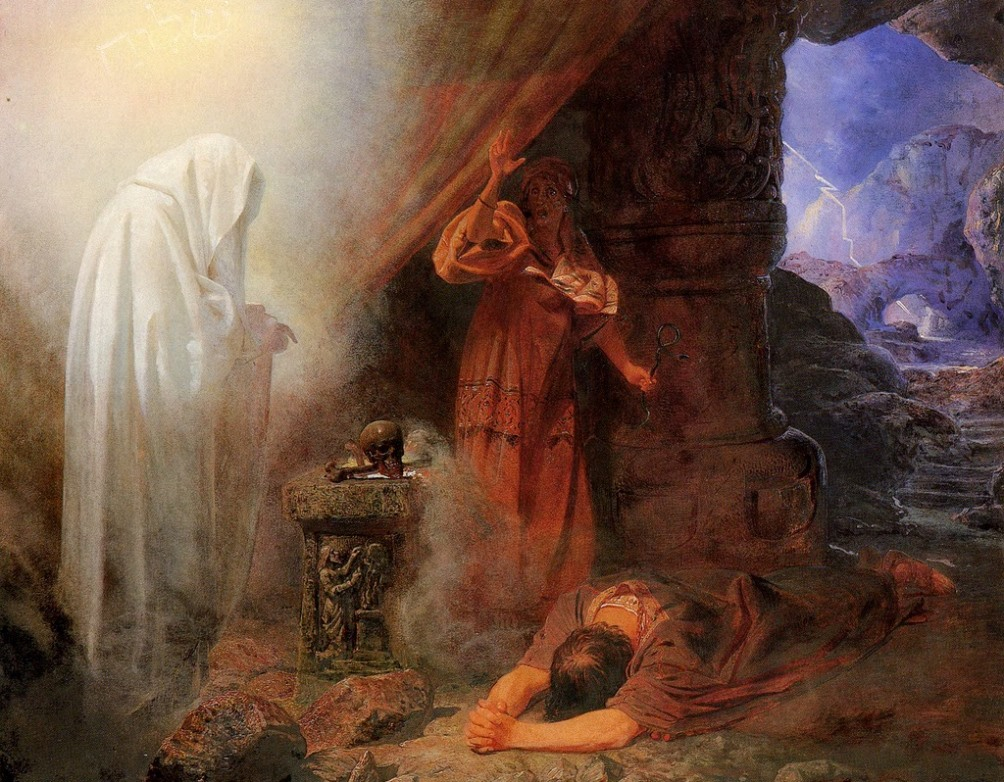
\includegraphics[width=0.85\linewidth]{image29.jpeg}
  \caption{Representação artística do conceito de Sheol como mundo subterrâneo dos mortos na tradição judaica antiga.}
  \label{fig:cap9-img2}
\end{figure}

Representação artística do conceito de Sheol como mundo subterrâneo dos mortos na tradição judaica antiga.


Essa concepção inicial do Sheol apresenta quatro características específicas:

Universalidade: Todos os mortos, justos e injustos, vão para o Sheol. Não há diferenciação moral explícita no destino póstumo.

Inatividade: Os habitantes do Sheol são frequentemente descritos como "sombras" (rephaim) que existem em um estado de consciência diminuída ou adormecida, sem vigor ou capacidade de louvar a Deus.

Irrevogabilidade: O Sheol é geralmente visto como um destino permanente, sem expectativa de retorno ou libertação (com raras exceções, como Enoque e Elias).

Ausência de elaboração moral: Não há menções explícitas de punição ou recompensa no Sheol; é simplesmente o destino comum a todos os humanos.

Esta concepção relativamente simples do além reflete uma teologia focada primariamente na vida terrena e na relação coletiva entre Deus e Israel. A recompensa divina e a punição eram vistas como ocorrendo principalmente neste mundo, através de bênçãos materiais, longevidade, prosperidade nacional e descendência numerosa para os justos, e calamidades, doença e derrota militar para os ímpios.

\section{A Transformação durante o Exílio e o Período do Segundo Templo}

A experiência traumática do exílio babilônico (586-539 a.C.) e as transformações sociais e religiosas subsequentes catalisaram mudanças significativas nas concepções judaicas do além. O contato com as religiões persas, particularmente o zoroastrismo com suas elaboradas doutrinas escatológicas, e mais tarde com o helenismo, expôs o pensamento judaico a novas possibilidades teológicas.

Gradualmente, nos textos tardios da Bíblia Hebraica e especialmente na literatura apocalíptica do período do Segundo Templo, emerge uma concepção mais diferenciada do além, que começa a incorporar elementos como:

Ressurreição dos mortos: Aparece explicitamente em Daniel 12:2: "E muitos dos que dormem no pó da terra ressuscitarão, uns para a vida eterna, e outros para vergonha e desprezo eterno."

Julgamento divino: Desenvolve-se a noção de um julgamento escatológico que determinará destinos diferentes para justos e ímpios.

Localização específica para punição: Gradualmente, o termo "Geena" (gy' hynwm, Gei Hinnom, o Vale de Hinnom) começa a ser utilizado para designar especificamente um local de punição para os ímpios, distinto do Sheol como destino universal.


\section{Geena: Do Vale Geográfico ao Símbolo de Punição}

A transformação da Geena de um local geográfico real a um símbolo de punição divina representa uma das evoluções mais fascinantes na escatologia judaica. Originalmente, Gei Hinnom (Vale de Hinnom) era um vale físico localizado ao sul de Jerusalém que adquiriu uma reputação sinistra por ser o local onde, segundo 2 Reis 23:10 e Jeremias 7:31, alguns israelitas praticaram sacrifícios infantis ao deus Moloch durante o período monárquico.


\begin{figure}[ht]
  \centering
  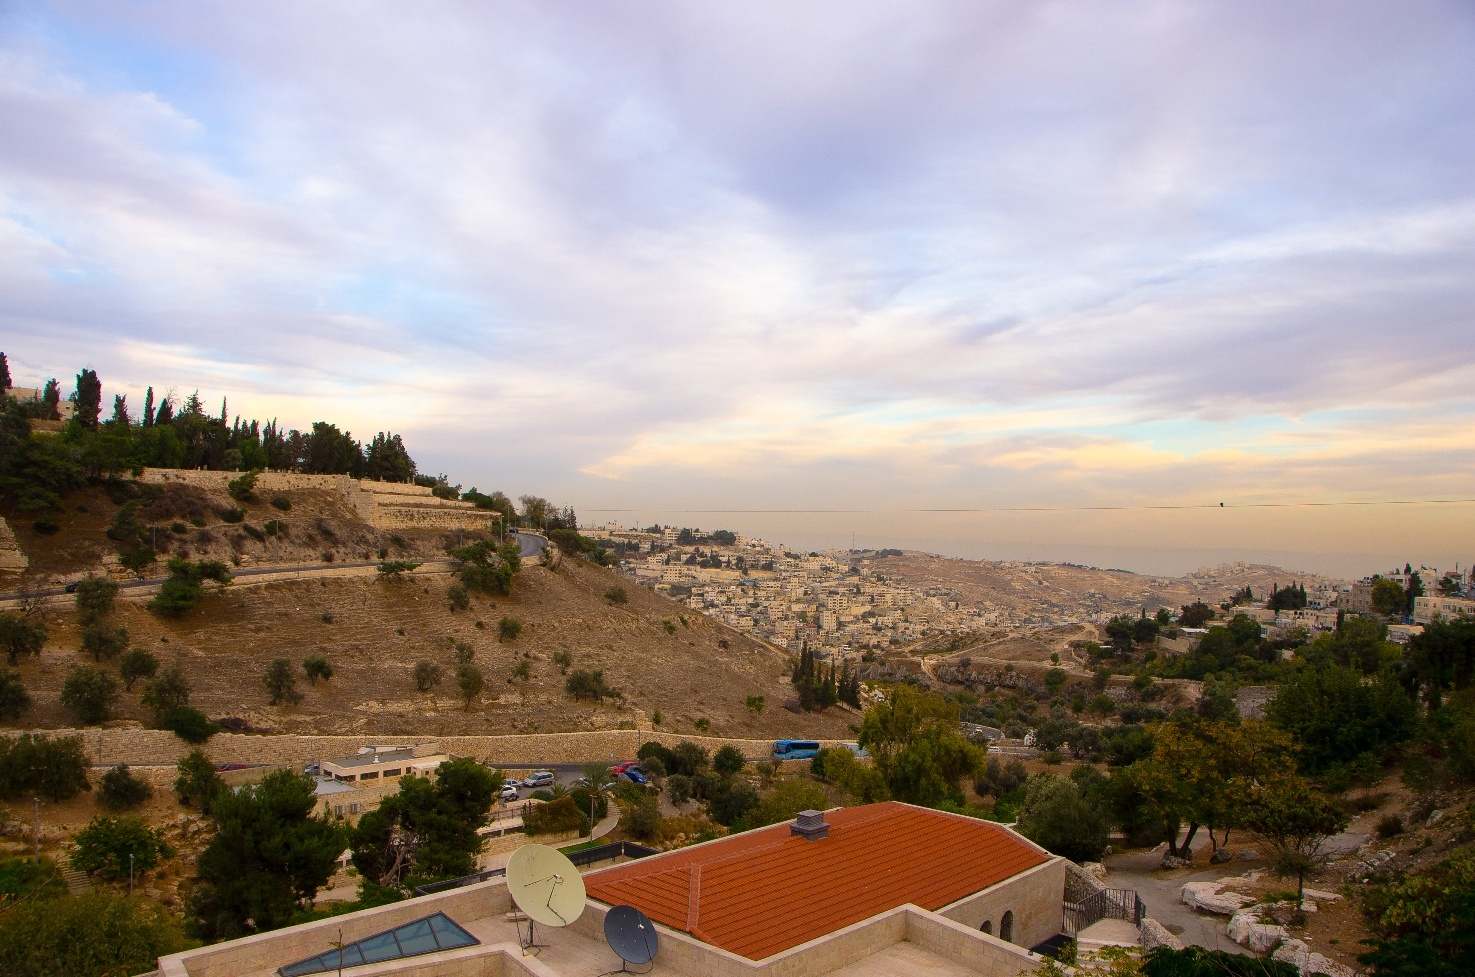
\includegraphics[width=0.85\linewidth]{image30.jpeg}
  \caption{Vale de Hinnom (Geena) na atualidade, ao sul de Jerusalém. Este local geográfico tornou-se um símbolo do inferno na tradição judaica tardia.}
  \label{fig:cap9-img3}
\end{figure}

Vale de Hinnom (Geena) na atualidade, ao sul de Jerusalém. Este local geográfico tornou-se um símbolo do inferno na tradição judaica tardia.

O rei Josias (640-609 a.C.) profanou este local como parte de suas reformas religiosas, e posteriormente o vale tornou-se um depósito de lixo onde fogo constante queimava os resíduos da cidade. Esta associação com fogo perpétuo, combinada com sua história macabra, fez da Geena uma poderosa metáfora para o local de punição divina na literatura apocalíptica judaica.

Em textos como 1 Enoque (um importante texto apocalíptico judaico do período do Segundo Templo), a Geena é descrita como um abismo de fogo onde os anjos caídos e os ímpios sofrerão punição eterna. Esta concepção representa uma ruptura significativa com a visão mais antiga do Sheol como destino universal e moralmente indiferenciado dos mortos.


\begin{figure}[ht]
  \centering
  \includegraphics[width=0.85\linewidth]{image31.png}
  \caption{Desenvolvimento do Conceito de Ressurreição e Julgamento}
  \label{fig:cap9-img4}
\end{figure}

Vista panorâmica do Vale de Hinnom (Geena), mostrando sua proximidade com a Cidade de Davi. O depósito de lixo em chamas que existia neste local forneceu a imagem do "fogo eterno" associado ao castigo divino.

\section{Desenvolvimento do Conceito de Ressurreição e Julgamento}

\subsection{Origens da Crença na Ressurreição}

A crença na ressurreição corporal, que viria a se tornar central para o judaísmo rabínico posterior e para o cristianismo, não era proeminente nos textos mais antigos da Bíblia Hebraica. Sua emergência gradual representa uma das transformações mais significativas na escatologia judaica.

Os primeiros indícios desta crença aparecem em textos proféticos tardios, particularmente em Isaías 26:19: "Os teus mortos viverão, os seus cadáveres ressuscitarão; despertai e exultai, vós que habitais no pó, porque o teu orvalho é orvalho de luz, e a terra dará à luz os seus mortos." E Ezequiel 37, com sua famosa visão do vale de ossos secos, que embora primariamente uma metáfora para a restauração nacional de Israel, estabelece o imaginário da ressurreição física.

No entanto, é em Daniel 12:2-3, escrito provavelmente durante a crise macabeia (c. 167-164 a.C.), que encontramos a declaração mais explícita e inequívoca da ressurreição na Bíblia Hebraica:

"E muitos dos que dormem no pó da terra ressuscitarão, uns para a vida eterna, e outros para vergonha e desprezo eterno. Os que forem sábios resplandecerão como o fulgor do céu; e os que converterem muitos à justiça, como as estrelas, sempre e eternamente."

\subsection{Julgamento Póstumo na Literatura Apocalíptica Judaica}

A literatura apocalíptica judaica, florescendo particularmente entre os séculos II a.C. e I d.C., desenvolveu consideravelmente as noções de julgamento póstumo e destinos diferenciados após a morte. Textos como 1 Enoque, 2 Baruc, 4 Esdras e os Testamentos dos Doze Patriarcas apresentam visões elaboradas do além, frequentemente incluindo descrições detalhadas de punições específicas para diferentes categorias de pecadores.


\begin{figure}[ht]
  \centering
  \includegraphics[width=0.85\linewidth]{image32.png}
  \caption{Manuscrito etíope do Livro de Enoque, um dos mais importantes textos apocalípticos judaicos que elaboram visões do além e do julgamento divino.}
  \label{fig:cap9-img5}
\end{figure}

Manuscrito etíope do Livro de Enoque, um dos mais importantes textos apocalípticos judaicos que elaboram visões do além e do julgamento divino.

Em 1 Enoque, particularmente, encontramos uma das primeiras descrições judaicas elaboradas de um julgamento escatológico e seus resultados. O texto descreve um "abismo de fogo" preparado para os anjos caídos e para os ímpios. Esta concepção representa uma evolução significativa em relação à visão mais antiga do Sheol como destino universal e moralmente indiferenciado.

O Livro dos Vigilantes (uma seção de 1 Enoque) descreve o local de punição:

"E vi um abismo profundo com colunas de fogo celestial, e vi nele colunas de fogo que desciam e cuja altura e profundidade não se podiam medir. Além deste abismo, vi um lugar sem o firmamento celeste sobre ele, nem o fundamento firme debaixo dele, nem água, nem aves, mas era um lugar vazio e terrível."

Estas descrições do lugar de punição em 1 Enoque apresentam características que seriam posteriormente desenvolvidas nas concepções cristãs e islâmicas do inferno: fogo, abismos profundos, separação completa de Deus, e tormento eterno.

\section{Literatura Apocalíptica Judaica e sua Visão do Inferno}

\subsection{1 Enoque e a Cartografia do Além}

O Livro de Enoque (1 Enoque), uma coleção de textos apocalípticos judaicos escritos entre os séculos III a.C. e I d.C., representa um dos desenvolvimentos mais significativos da escatologia judaica e contém algumas das descrições mais detalhadas do além no judaísmo antigo. O texto, preservado completo apenas em ge'ez (etíope), exerceu influência considerável sobre o cristianismo primitivo e foi citado na Epístola de Judas do Novo Testamento.


\begin{figure}[ht]
  \centering
  \includegraphics[width=0.85\linewidth]{image33.jpeg}
  \caption{Fragmento do Livro de Enoque encontrado entre os Manuscritos do Mar Morto, demonstrando a importância deste texto apocalíptico no judaísmo do período do Segundo Templo.}
  \label{fig:cap9-img6}
\end{figure}

Fragmento do Livro de Enoque encontrado entre os Manuscritos do Mar Morto, demonstrando a importância deste texto apocalíptico no judaísmo do período do Segundo Templo.

Enoque apresenta uma cartografia detalhada do além, descrevendo as jornadas do patriarca através de várias regiões celestiais e infernais. No texto, o além não é simplesmente um local homogêneo, mas um complexo de regiões distintas com funções específicas.

\subsection{Os Manuscritos do Mar Morto e as Crenças Essênias}

Os Manuscritos do Mar Morto, descobertos nas cavernas de Qumran entre 1947 e 1956, fornecem insights valiosos sobre as crenças escatológicas de um grupo judaico sectário frequentemente identificado com os essênios. Estes textos, datados aproximadamente do século II a.C. ao I d.C., revelam uma comunidade intensamente preocupada com o julgamento final e o destino póstumo.


\begin{figure}[ht]
  \centering
  \includegraphics[width=0.85\linewidth]{image34.jpeg}
  \caption{Ruínas de Qumran, onde foram encontrados os Manuscritos do Mar Morto, incluindo textos apocalípticos que detalham concepções elaboradas do além e do julgamento divino.}
  \label{fig:cap9-img7}
\end{figure}

Ruínas de Qumran, onde foram encontrados os Manuscritos do Mar Morto, incluindo textos apocalípticos que detalham concepções elaboradas do além e do julgamento divino.

A "Regra da Comunidade" (1QS), um dos textos mais significativos de Qumran, descreve o destino dos "filhos das trevas":

"Para os ídolos da abominação está reservada a punição do fogo eterno. E o espírito de perversidade que há dentro deles, a humilhação nas trevas do fogo eterno, a angústia da destruição no inferno das trevas, todos os seus tempos ao longo das gerações, com aflições dolorosas e amargura calamitosa nas moradas das trevas, até sua destruição, sem que haja um remanescente ou sobrevivente entre eles."

\section{Variações nas Concepções Judaicas ao Longo da História}

\subsection{Diferenças entre Fariseus, Saduceus e Essênios}

O judaísmo do período do Segundo Templo não era monolítico, mas caracterizado por uma diversidade de movimentos religiosos com diferentes interpretações teológicas, incluindo variações significativas nas concepções do além. O historiador judeu-romano Flávio Josefo (c. 37-100 d.C.) oferece um relato valioso destas diferenças em sua obra "Antiguidades Judaicas".

Segundo Josefo, os saduceus, predominantemente associados à aristocracia sacerdotal, rejeitavam tanto a crença na ressurreição quanto na imortalidade da alma. Para eles, a justiça divina operava exclusivamente dentro dos limites da vida terrena, e não havia existência consciente após a morte.

Os fariseus, por outro lado, aceitavam a ressurreição dos mortos e desenvolveram concepções mais elaboradas de recompensa e punição no além. Josefo escreve que eles acreditavam que "as almas têm poder imortal nelas" e que "há sob a terra recompensas e punições para aqueles que foram virtuosos ou viciosos na vida".

Os essênios, possivelmente associados à comunidade de Qumran, sustentavam crenças ainda mais desenvolvidas sobre o além. Josefo relata que eles acreditavam que "os corpos são corruptíveis... mas as almas são imortais e continuam para sempre" e que após a morte "as boas almas recebem uma habitação além do oceano... enquanto as más almas encontram um lugar de punição cheio de punições incessantes".

\subsection{O Desenvolvimento do Gehinom na Literatura Rabínica}

Após a destruição do Segundo Templo em 70 d.C., o judaísmo rabínico emergiu como a corrente dominante, preservando e desenvolvendo muitos elementos da tradição farisaica. Na vasta literatura rabínica, incluindo a Mishná, o Talmude e os Midrashim, encontramos um desenvolvimento significativo das concepções do além, particularmente a elaboração do conceito de Gehinom (Geena).

Uma característica distintiva da concepção rabínica do Gehinom é seu caráter geralmente temporário. Diferente das concepções cristãs posteriores do inferno como punição eterna, o Gehinom rabínico funciona predominantemente como um local de purificação temporária. O Talmude sugere que, exceto para os piores pecadores, a estadia no Gehinom é limitada:

"Os pecadores de Israel em seus corpos e os pecadores das nações do mundo em seus corpos descem ao Gehinom e são punidos lá por doze meses. Após doze meses, seus corpos são consumidos e suas almas são queimadas, e o vento espalha [suas cinzas] sob as plantas dos pés dos justos..." (Rosh Hashanah 17a)


A evolução das concepções judaicas do além representa uma transformação notável de uma visão inicial relativamente simples e moralmente indiferenciada do Sheol para uma compreensão complexa e moralmente estruturada do destino pós-morte. Este desenvolvimento não foi linear nem uniforme, mas refletiu as experiências históricas de Israel, o contato com outras culturas, e a contínua reflexão teológica sobre a natureza da justiça divina.

Vários elementos específicos desta tradição exerceram influência duradoura nas concepções posteriores do inferno:

A diferenciação moral do além, com destinos distintos para justos e ímpios, estabeleceu um fundamento conceitual para visões posteriores de céu e inferno.

A associação do fogo com punição divina, desde a Geena histórica como depósito de lixo em chamas até sua reinterpretação como local de punição cósmica, tornou-se um símbolo central nas representações posteriores do inferno.

O princípio de correspondência entre pecado e punição, desenvolvido particularmente na literatura apocalíptica e rabínica, influenciou profundamente as concepções cristãs e islâmicas de justiça divina.

A tensão entre interpretações literais e alegóricas do além, presente nas tradições rabínicas e filosóficas, continuou a caracterizar debates teológicos sobre o inferno nas tradições abraâmicas.


\begin{figure}[ht]
  \centering
  \includegraphics[width=0.85\linewidth]{image35.jpeg}
  \caption{Confluência dos vales de Hinnom e Cedrom, ao sul de Jerusalém, cuja geografia alimentou o simbolismo posterior da Geena.}
  \label{fig:cap9-img8}
\end{figure}

A confluência do Vale de Hinnom com o Vale de Cedrom ao sul de Jerusalém. Esta geografia real forneceu o simbolismo para concepções escatológicas que influenciariam profundamente o pensamento religioso ocidental.

Talvez o legado mais significativo das concepções judaicas do inferno seja a transformação gradual de um destino universal e inevitável (Sheol) em um local de punição moral diferenciada (Gehinom), refletindo uma evolução paralela na compreensão da relação entre Deus e a humanidade: de um enfoque primariamente nacional e coletivo para uma ênfase crescente na responsabilidade moral individual e no destino pessoal.

Esta evolução estabeleceu fundamentos conceituais cruciais para o desenvolvimento das doutrinas cristãs e islâmicas do inferno, que serão exploradas nos próximos capítulos. Ao mesmo tempo, a persistência de interpretações distintas e a diversidade de opiniões dentro da tradição judaica ilustram a complexidade e multivalência das concepções do além nas tradições religiosas vivas.


% --- Capítulo 10 O Inferno Cristão: Da Parábola à Teologia ---
\chapter[Inferno Cristão Primitivo]{O Inferno Cristão: Da Parábola à Teologia}
\epigraph{A concepção cristã do inferno surgiu em convergência de tradições judaicas, greco-romanas e orientais --- mas desenvolveu características distintivas que viriam a moldar profundamente o imaginário ocidental sobre o pós-vida, desde as parábolas de Jesus até a sistematização dos Padres da Igreja.}

A concepção cristã do inferno surgiu em um contexto de convergência cultural, herdando elementos das tradições judaicas, greco-romanas e orientais. Diferentemente de suas origens, entretanto, o inferno cristão desenvolveu características distintivas que viriam a moldar profundamente o imaginário ocidental sobre o pós-vida. Este capítulo explora a trajetória dessa ideia, desde seu nascimento nas parábolas de Jesus até sua sistematização teológica pelos Padres da Igreja nos primeiros séculos do cristianismo.

A transformação do conceito de inferno foi uma das mais significativas evoluções teológicas do cristianismo primitivo. Partindo de referências ocasionais e metafóricas nos ensinamentos de Jesus, o inferno gradualmente adquiriu contornos de um sistema elaborado de punição divina, com geografia específica, diferentes níveis de sofrimento e uma integração completa à cosmovisão cristã. Essa evolução revela não apenas mudanças teológicas, mas também o desenvolvimento da identidade cristã em um mundo predominantemente pagão.

\section{As Parábolas de Jesus e o Inferno}

Os evangelhos apresentam Jesus utilizando imagens de punição pós-morte em diversos contextos, embora sempre de forma sucinta e frequentemente metafórica. Destacam-se suas referências à Geena (a versão grega do hebraico Gehenna), ao "fogo eterno" e à "escuridão exterior, onde haverá choro e ranger de dentes". Estas alusões, contudo, eram menos detalhadas que as elaborações posteriores, servindo primariamente como alertas morais dentro de um contexto judaico já familiarizado com a ideia de castigo divino.

\subsection{A Geena como Símbolo}

A Geena, mencionada doze vezes nos evangelhos sinóticos, referia-se originalmente ao Vale de Hinom, nos arredores de Jerusalém. Este local carregava uma história sinistra: fora usado para sacrifícios de crianças ao deus Moloque durante o período da monarquia israelita. Posteriormente, tornou-se um depósito de lixo da cidade, onde o fogo queimava continuamente. Jesus apropriou-se dessa imagem vívida e culturalmente significativa para seus ouvintes:

"Se tua mão te faz tropeçar, corta-a; é melhor entrares na vida aleijado do que, tendo as duas mãos, ires para a Geena, para o fogo inextinguível."

Marcos 9:43

O uso que Jesus faz da Geena já sugere um simbolismo de purificação pelo fogo e separação dos elementos impuros, temas que seriam amplificados pela teologia posterior. A associação entre lixo, impureza, fogo perpétuo e punição estabeleceu uma conexão conceitual poderosa que permaneceria central ao desenvolvimento da doutrina cristã do inferno.

\subsection{A Parábola do Rico e Lázaro}

Dentre todos os ensinamentos de Jesus, a parábola do Rico e Lázaro (Lucas 16:19-31) oferece a descrição mais detalhada de um estado de punição pós-morte. Esta narrativa apresenta elementos que seriam fundamentais para a posterior concepção cristã do inferno:


\begin{figure}[ht]
  \centering
  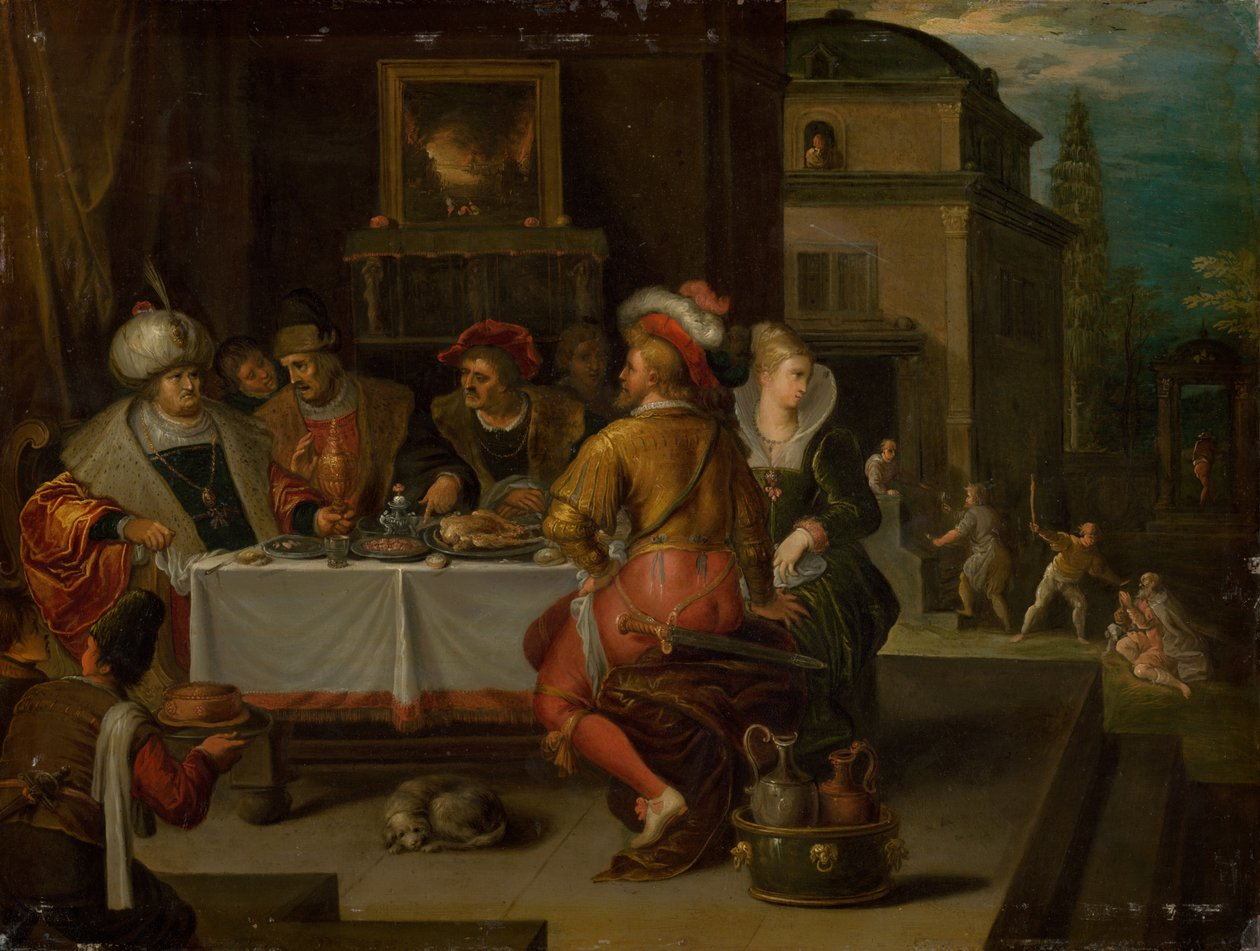
\includegraphics[width=0.85\linewidth]{image36.jpeg}
  \caption{A parábola do homem rico e do mendigo Lázaro, pintura de Frans Francken (1615).}
  \label{fig:cap10-img1}
\end{figure}

A parábola do homem rico e do mendigo Lázaro, pintura de Frans Francken (1615).

Na parábola, um homem rico que ignorou o sofrimento do mendigo Lázaro encontra-se, após a morte, "em tormentos" (\ensuremath{\epsilon}\ensuremath{\nu} \ensuremath{\beta}\ensuremath{\alpha}\ensuremath{\sigma}\ensuremath{\acute{alpha}}\ensuremath{\nu}o\ensuremath{\iota}\ensuremath{\varsigma}), consciente de sua situação, capaz de ver Abraão e Lázaro "ao longe", sentindo sede intensa e sendo atormentado por "esta chama" (\ensuremath{\tau}\ensuremath{\bar{eta}} \ensuremath{\phi}\ensuremath{\lambda}o\ensuremath{\gamma}\ensuremath{\grave{iota}} \ensuremath{\tau}\ensuremath{\alpha}\ensuremath{\acute{upsilon}}\ensuremath{\tau}\ensuremath{\eta}). A narrativa também estabelece uma "grande separação" (\ensuremath{\chi}\ensuremath{\acute{alpha}}\ensuremath{\sigma}\ensuremath{\mu}\ensuremath{\alpha} \ensuremath{\mu}\ensuremath{\acute{epsilon}}\ensuremath{\gamma}\ensuremath{\alpha}) intransponível entre os justos e os condenados.

Embora muitos teólogos modernos interpretem esta narrativa como uma parábola alegórica e não como uma descrição literal da geografia do além, sua influência na formação da concepção cristã do inferno foi inegável. Os elementos de consciência após a morte, sofrimento físico pelo fogo, separação eterna e impossibilidade de redenção tornaram-se centrais ao imaginário cristão sobre o inferno.

"Filho, lembra-te de que recebeste os teus bens durante a tua vida, e Lázaro igualmente, os males; agora, porém, ele está consolado, e tu, em tormentos. E, além de tudo, existe um grande abismo entre nós e vós, de sorte que os que querem passar daqui para vós outros não podem, nem os de lá passar para nós."

Lucas 16:25-26

\section{A Emergência da Doutrina no Cristianismo Primitivo}

A transição das referências ocasionais de Jesus a um sistema teológico estruturado ocorreu gradualmente durante os primeiros séculos da era cristã. Esse desenvolvimento foi estimulado por diversos fatores: a necessidade de consolação em tempos de perseguição, o desejo de justiça divina retributiva, a apropriação de elementos culturais greco-romanos e o confronto com heresias emergentes.

\subsection{Referências no Novo Testamento}

Além das palavras de Jesus, outros escritos do Novo Testamento expandiram o conceito de punição eterna. O livro do Apocalipse, com sua vívida imagética do "lago de fogo e enxofre", onde "o diabo, a besta e o falso profeta serão atormentados dia e noite, pelos séculos dos séculos" (Apocalipse 20:10), forneceu elementos adicionais ao imaginário infernal. O apóstolo Paulo, embora menos explícito em suas descrições, fala da "ira vindoura" e da "ruína eterna, banidos da face do Senhor e da glória do seu poder" (2 Tessalonicenses 1:9).

Essas referências, ainda que esparsas e nem sempre consistentes entre si, constituíram a base escriturística sobre a qual os primeiros teólogos cristãos construiriam sua doutrina do inferno. A diversidade de terminologia e imagens no Novo Testamento -- Geena, Hades, lago de fogo, trevas exteriores, destruição eterna -- seria posteriormente harmonizada em um sistema teológico mais coerente.

\subsection{O Apocalipse de Pedro}

Um dos textos mais influentes para o desenvolvimento da concepção cristã do inferno não foi incorporado ao cânon bíblico. O Apocalipse de Pedro, escrito provavelmente entre 100-150 d.C., contém a primeira descrição cristã detalhada das punições infernais. Apesar de não ter sido incluído no cânon final do Novo Testamento, este texto foi amplamente lido nas comunidades cristãs primitivas e citado por autores como Clemente de Alexandria.


\begin{figure}[ht]
  \centering
  \includegraphics[width=0.85\linewidth]{image37.png}
  \caption{Página de um manuscrito do Apocalipse de Pedro, texto apócrifo que influenciou significativamente a concepção cristã do inferno.}
  \label{fig:cap10-img2}
\end{figure}

Página de um manuscrito do Apocalipse de Pedro, texto apócrifo que influenciou significativamente a concepção cristã do inferno.

No Apocalipse de Pedro, Jesus revela a seu discípulo uma visão detalhada dos castigos do inferno, onde diferentes pecados recebem punições específicas e adequadas à sua natureza -- um princípio que seria conhecido como contrapasso (castigo por contraste ou analogia) e mais tarde magnificamente elaborado por Dante em sua Divina Comédia:

"E havia homens e mulheres com os lábios cortados e fogo em suas bocas. Estes eram os falsos testemunhos [...] E outros homens e mulheres eram lançados do alto de um precipício e forçados a subir novamente, apenas para serem empurrados novamente pelos seus torturadores. Estes eram os que profanaram seus corpos agindo como mulheres; e as mulheres que estavam com eles eram as que deitaram umas com as outras como um homem com uma mulher."

Apocalipse de Pedro, fragmento aqueniano

Este texto apresenta características fundamentais que seriam incorporadas à doutrina posterior: punições físicas específicas para diferentes categorias de pecados, a eternidade dos tormentos e o papel do fogo como principal instrumento de punição. A detalhada descrição de torturas físicas no Apocalipse de Pedro serviu como base para muitas representações artísticas e literárias posteriores do inferno.

A ideia cristã do inferno nasceu de metáforas simples, mas carregadas de força simbólica, e foi progressivamente transformada em uma doutrina elaborada, com profundos impactos na teologia, na pastoral e no imaginário ocidental.

Das advertências parabólicas de Jesus à sistematização pelos Padres da Igreja, o inferno passou de imagem moral a arquitetura teológica: espaço de justiça retributiva, de separação absoluta e de tormentos eternos.

Esse processo revela não apenas a plasticidade do cristianismo diante de tradições culturais distintas, mas também sua capacidade de criar uma visão do pós-vida que serviu, ao mesmo tempo, como consolo aos fiéis perseguidos e como instrumento de disciplina espiritual. O inferno, assim, tornou-se um dos símbolos mais duradouros da identidade cristã e do modo como o Ocidente aprendeu a pensar sobre justiça, pecado e eternidade.


% --- Capítulo 11: A Sistematização Teológica dos Padres da Igreja ---
\chapter[Sistematização Patrística]{A Sistematização Teológica dos Padres da Igreja}
\index{Orígenes}\index{Apokatastasis}


\epigraph{Durante os séculos II a V, os Padres da Igreja desenvolveram reflexões teológicas mais sistemáticas sobre o inferno, consolidando elementos dispersos das Escrituras e da tradição oral em uma doutrina coerente. Este período foi marcado por intensos debates sobre a natureza, duração e propósito das punições infernais.}


\section{Visões Divergentes: Universalismo versus Inferno Eterno}

Um dos primeiros debates significativos envolveu a possibilidade de salvação universal (apokatastasis) defendida por Orígenes de Alexandria (c. 185-254). Baseando-se em passagens como 1 Coríntios 15:28 ("para que Deus seja tudo em todos"), Orígenes propôs que todos os seres, incluindo o próprio Satanás, seriam eventualmente purificados e restaurados à comunhão com Deus. Para ele, o fogo do inferno era purificatório e terapêutico, não meramente punitivo:

"Acredito que a bondade de Deus, por meio de seu Cristo, conduzirá toda a criação a um único fim [...] Quando todos os inimigos tiverem sido submetidos a Cristo, Cristo também se submeterá ao Pai, e Deus será tudo em todos."

Orígenes, De Principiis, 3.6.3

Contrapondo-se a esta visão, Tertuliano (c. 160-225) defendia a eternidade dos tormentos infernais como parte essencial da justiça divina. Em seu tratado De Spectaculis (Sobre os Espetáculos), ele chega a descrever o espetáculo do Juízo Final como superior a qualquer entretenimento romano, onde os cristãos poderão contemplar os sofrimentos eternos de seus perseguidores:

"Que espetáculo está próximo! Como eu vou admirar, como vou rir, como vou regozijar-me, como vou exultar, quando contemplar tantos e tão grandes reis, de quem se dizia estarem no céu, gemendo nas mais profundas trevas com Júpiter e seus adeptos! [...] Prefiro fixar meu olhar insaciável naqueles cuja raiva e furor se exercitaram na perseguição do nome do Senhor."

Tertuliano, De Spectaculis, XXX

Esta divergência entre o universalismo de Orígenes e o infernalismo de Tertuliano representou um dos primeiros grandes debates teológicos sobre o destino final dos pecadores. Com o tempo, a posição de Tertuliano prevaleceria na ortodoxia ocidental, enquanto as ideias de Orígenes seriam condenadas no Segundo Concílio de Constantinopla (553).

\section{Santo Agostinho e a Consolidação da Doutrina}

A contribuição mais decisiva para a teologia ocidental do inferno veio de Santo Agostinho de Hipona (354-430). Em suas obras A Cidade de Deus e Enchiridion, Agostinho desenvolveu uma doutrina abrangente do inferno que sintetizava elementos bíblicos, filosóficos e das tradições patrísticas anteriores.


\begin{figure}[ht]
  \centering
  \includegraphics[width=0.85\linewidth]{image38.jpeg}
  \caption{Detalhe do Inferno no Juízo Final, mosaico de Coppo di Marcovaldo (1225), refletindo a concepção agostiniana do inferno que perdurou na arte cristã medieval.}
  \label{fig:cap11-img1}
\end{figure}

Detalhe do Inferno no Juízo Final, mosaico de Coppo di Marcovaldo (1225), refletindo a concepção agostiniana do inferno que perdurou na arte cristã medieval.

Para Agostinho, o inferno era:

Eterno em duração: Rejeitando explicitamente o universalismo de Orígenes, Agostinho insistiu que as punições dos condenados seriam sem fim, baseando-se em Mateus 25:41,46.

Corporalmente real: Após a ressurreição, os condenados sofreriam em corpos reais, embora miraculosamente capazes de suportar o tormento eterno sem serem consumidos.

Justo e proporcional: As punições variariam em intensidade de acordo com os pecados cometidos em vida.

Essencialmente privativo: O sofrimento fundamental do inferno seria a separação definitiva de Deus, fonte de todo bem e felicidade.

Agostinho também desenvolveu a base teológica para o que mais tarde seria chamado de poena damni (pena de dano -- a privação da visão beatífica de Deus) e poena sensus (pena de sentido -- os tormentos físicos), distinção que seria fundamental para a escatologia medieval.

"As penas do inferno serão diferentes em intensidade; cada um será punido de acordo com seus crimes. No entanto, o menor castigo que qualquer pessoa sofrerá no inferno será mais terrível que o pior sofrimento que alguém poderia suportar nesta vida."

Santo Agostinho, A Cidade de Deus, XXI, 16

A visão agostiniana predominaria no cristianismo ocidental por mais de um milênio, influenciando profundamente a teologia, a arte, a literatura e a cultura popular. Sua concepção de inferno eterno e corporalmente real estabeleceu-se como doutrina oficial da Igreja no século VI, após as condenações formais ao universalismo origenista.

\section{Representações Artísticas Primitivas}

A arte cristã primitiva foi inicialmente reticente em representar o inferno de forma explícita. Nos primeiros séculos, as catacumbas e basílicas paleocristãs privilegiavam imagens de salvação e esperança, como o Bom Pastor ou o Cristo Triunfante. No entanto, a partir do século V, começam a surgir representações visuais do inferno que refletem a crescente elaboração teológica do conceito.

\subsection{Mosaicos Bizantinos e o Juízo Final}

Os mais antigos exemplos sobreviventes de representações artísticas do inferno cristão encontram-se em mosaicos bizantinos do século VI em diante. Nestas obras, o inferno aparece geralmente como parte da cena do Juízo Final, mostrando Cristo em majestade separando os justos dos condenados.


\begin{figure}[ht]
  \centering
  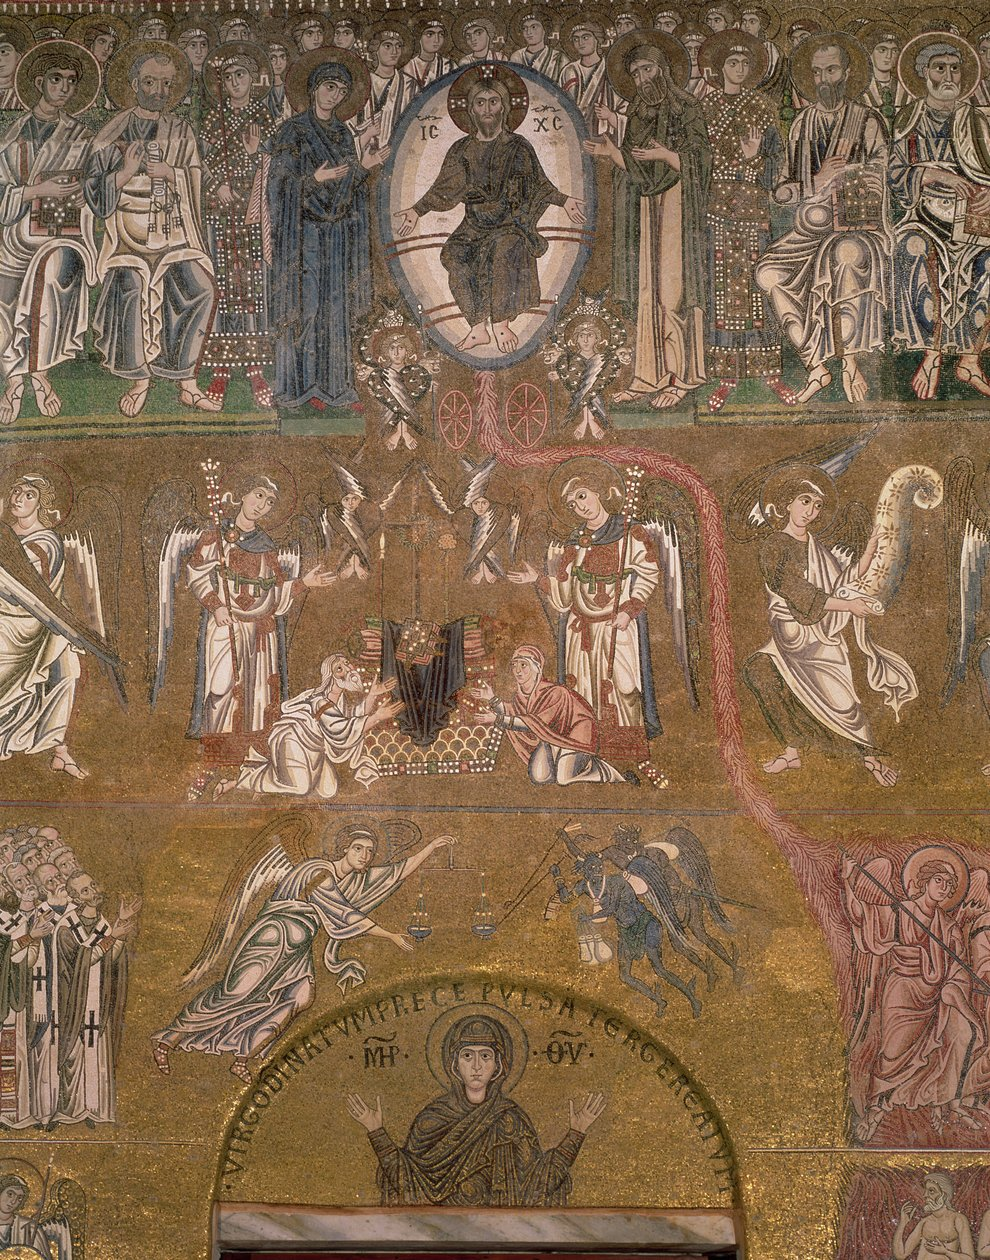
\includegraphics[width=0.85\linewidth]{image39.jpeg}
  \caption{O Juízo Final, detalhe do Julgamento de Cristo, mosaico bizantino do século XII. A cena do julgamento se tornaria inseparável da representação do inferno na arte cristã.}
  \label{fig:cap11-img2}
\end{figure}

O Juízo Final, detalhe do Julgamento de Cristo, mosaico bizantino do século XII. A cena do julgamento se tornaria inseparável da representação do inferno na arte cristã.

Nestes mosaicos, o inferno é tipicamente representado como um abismo escuro ou um rio de fogo onde os condenados são lançados, frequentemente com demônios arrastando-os para baixo. A iconografia bizantina estabeleceu muitos elementos visuais que se tornariam convencionais nas representações posteriores do inferno: o fogo eterno, os demônios torturadores, os condenados nus demonstrando desespero, e a organização hierárquica das punições.

Um exemplo notável é o mosaico do Juízo Final na Catedral de Torcello (século XII), onde o inferno é representado em seis compartimentos horizontais, cada um dedicado a diferentes categorias de pecadores e punições -- uma organização que antecipa a geografia infernal da Divina Comédia de Dante.

\subsection{Manuscritos Iluminados e a Propagação Visual}

A partir do século IX, manuscritos iluminados começaram a incluir representações mais detalhadas do inferno, especialmente em cópias do Apocalipse e em livros de horas. Estas imagens, inicialmente reservadas à elite eclesiástica e aristocrática, gradualmente se difundiram e contribuíram para a popularização da visão agostiniana do inferno.

Um exemplar significativo é o Utrecht Psalter (c. 830), cujas ilustrações incluem demônios torturando condenados em um caldeirão fervente -- uma imagem que se tornaria icônica na representação medieval do inferno. Estas representações visuais não apenas refletiam a doutrina teológica, mas também a reforçavam e popularizavam entre os fiéis, a maioria dos quais era iletrada.

\section{A Função Social e Teológica do Inferno Primitivo}

O desenvolvimento da doutrina do inferno no cristianismo primitivo serviu a várias funções sociais e teológicas importantes, que ajudam a explicar sua rápida aceitação e elaboração:

Para os cristãos dos primeiros séculos, frequentemente perseguidos e marginalizados, a doutrina do inferno oferecia a garantia de uma justiça final que compensaria os sofrimentos presentes. A visão de imperadores, magistrados e perseguidores pagãos sofrendo eternamente -- como vividamente descrito por Tertuliano -- proporcionava consolo psicológico a comunidades oprimidas.

Esta função do inferno como mecanismo de justiça cósmica é particularmente evidente nos relatos de martírio, onde os santos frequentemente profetizam as punições infernais que aguardam seus torturadores. O Martírio de Policarpo (c. 155-160 d.C.), por exemplo, contrasta o "fogo temporal" da fogueira do mártir com o "fogo eterno" reservado aos perseguidores.

\subsection{Instrumento de Controle Social e Moral}

À medida que o cristianismo se expandia e se institucionalizava, a doutrina do inferno tornou-se um poderoso instrumento de controle social e moral. A ameaça de punição eterna servia como freio contra transgressões que muitas vezes escapariam à justiça humana, como pecados secretos ou perpetrados pelos poderosos.

Quando o Império Romano se cristianizou, após o Édito de Milão (313), a ênfase no inferno como lugar de punição para perseguidores diminuiu, sendo substituída gradualmente pela ênfase no inferno como destino dos hereges, apóstatas e pecadores impenitentes dentro da própria comunidade cristã.

\subsection{Resposta às Heresias e Consolidação Doutrinária}

O desenvolvimento da doutrina do inferno também serviu como resposta a vários movimentos considerados heréticos, como o gnosticismo (que negava a realidade do corpo e, portanto, de punições corporais após a morte) e o maniqueísmo (que propunha um dualismo radical entre bem e mal).

A insistência agostiniana na realidade corporal do inferno, por exemplo, constituía uma reafirmação da doutrina da ressurreição do corpo contra tendências gnósticas. Da mesma forma, sua ênfase na soberania divina até mesmo sobre o inferno era uma resposta ao dualismo maniqueísta.

\begin{longtable}{@{}p{2.5cm}p{5.4cm}p{6.0cm}@{}}
\caption{Desenvolvimento da doutrina cristã do inferno.}\\
\toprule
\textbf{Período} & \textbf{Desenvolvimento} & \textbf{Textos e autores} \\
\midrule
\endfirsthead
\toprule
\textbf{Período} & \textbf{Desenvolvimento} & \textbf{Textos e autores} \\
\midrule
\endhead
30--90 d.C. & Referências simbólicas à Geena e ao fogo eterno & Evangelhos Sinóticos e parábola do rico e Lázaro \\
90--150 d.C. & Primeiras descrições detalhadas das punições & Apocalipse de João e Apocalipse de Pedro \\
150--250 d.C. & Debate sobre a eternidade das penas & Tertuliano e Orígenes \\
250--400 d.C. & Sistematização da doutrina do inferno & Lactâncio e Efrém da Síria \\
400--550 d.C. & Consolidação da visão ocidental & Santo Agostinho e Gregório Magno \\
\bottomrule
\end{longtable}

A evolução do conceito de inferno no cristianismo primitivo representa um dos processos mais significativos de desenvolvimento teológico dos primeiros cinco séculos da Igreja. Partindo de alusões metafóricas e parábolas nos ensinamentos de Jesus, a doutrina do inferno expandiu-se em um sistema teológico elaborado, com profundas implicações para a escatologia, a soteriologia e a ética cristã.

Este desenvolvimento não foi apenas uma questão de especulação teológica abstrata, mas refletiu as condições sociais, políticas e culturais das primeiras comunidades cristãs. A transformação do inferno de um símbolo de advertência moral para uma realidade cósmica central à visão cristã do mundo demonstra como doutrinas religiosas respondem a necessidades históricas específicas.

O inferno cristão, tal como concebido pelos Padres da Igreja, serviria como base para elaborações teológicas e artísticas ainda mais detalhadas durante a Idade Média. Entretanto, já no período patrístico, suas características essenciais estavam estabelecidas: eternidade das punições, realidade corporal dos tormentos, proporcionalidade das penas aos pecados, e centralidade do fogo como instrumento de castigo.

A imagem do inferno que emerge dos primeiros séculos cristãos é, assim, um testemunho da profunda preocupação da Igreja primitiva com questões de justiça divina, responsabilidade moral e destino último da alma -- temas que continuariam a ocupar um lugar central na teologia cristã pelos séculos vindouros.


% --- Capítulo 12: Desenvolvimentos Patrísticos Orientais ---
\chapter[Patrística Oriental]{Desenvolvimentos Patrísticos Orientais}
\index{Theosis}


\epigraph{Os Padres Orientais --- de Clemente de Alexandria a Gregório de Nissa --- desenvolveram uma escatologia distinta, enfatizando a finalidade restauradora do castigo divino (apokatastasis) e a misericórdia soberana de Deus em tensão criativa com a tradição ocidental.}

Os desenvolvimentos teológicos dos Padres da Igreja orientais constituem uma tradição teológica distinta, oferecendo perspectivas únicas sobre escatologia e punição eterna, frequentemente em contraste com as sínteses latinas contemporâneas. Essa tradição floresceu em culturas diversas --- siríaca, copta, bizantina, armênia e georgiana --- integrando elementos da filosofia grega, de tradições semíticas orientais e de experiências místicas. Como resultado, surgiram sínteses escatológicas sofisticadas que enfatizam a transformação espiritual e a deificação (theosis) em vez de uma concepção de inferno centrada na punição estritamente retributiva. Nos desenvolvimentos orientais, a misericórdia divina e a possibilidade de redenção tendem a ocupar papel central, em contraste com a ênfase ocidental medieval na justiça retributiva e no castigo eterno.


\section{Tradição Siríaca: Teologia Poética e Misericórdia Divina}

A tradição siríaca, exemplificada pela Escola de Edessa e por figuras como Santo Efrém, o Sírio (306--373), desenvolveu uma teologia poética rica em imagens escatológicas. Nas suas homilias e hinos, Efrém descreve vividamente o Paraíso e o Inferno, construindo uma “geografia” espiritual que contrasta um Paraíso estratificado com regiões de punição para os pecadores. Importante notar, porém, que mesmo ao pintar os tormentos infernais, a perspectiva siríaca enfatiza a compaixão divina e a possibilidade de intercessão pelos mortos. Nos Hinos sobre o Paraíso, Efrém apresenta um Paraíso com múltiplos níveis de glória, enquanto o Inferno é retratado como afastamento da luz divina --- contudo, a misericórdia de Deus sempre permeia essas visões.


\begin{figure}[ht]
  \centering
  \includegraphics[width=0.85\linewidth]{image40.jpeg}
  \caption{Santo Efrém, o Sírio (306-373) - Mosaico bizantino do Mosteiro de Nea Moni. Efrém desenvolveu uma teologia poética distintiva que enfatizava a misericórdia divina sobre a punição retributiva.}
  \label{fig:cap12-img1}
\end{figure}

Santo Efrém, o Sírio (306-373) - Mosaico bizantino do Mosteiro de Nea Moni. Efrém desenvolveu uma teologia poética distintiva que enfatizava a misericórdia divina sobre a punição retributiva.

Essa ênfase contrasta com a teologia latina contemporânea (por exemplo, a de Santo Agostinho) que tendia a sublinhar a retribuição justa pelos pecados. Em síntese, a teologia siríaca patrística valoriza a esperança na clemência divina, refletida na prática litúrgica de orar pelos defuntos e na confiança de que as almas podem ser transformadas pela graça, mesmo após a morte.

No Egito, a tradição copta desenvolveu-se absorvendo elementos das crenças faraônicas sobre o pós-vida, adaptando-os à teologia cristã. Escritos apócrifos como o Apocalipse Copta de Pedro (datado possivelmente do século III ou IV, com fragmentos preservados em Akhmim) descrevem em detalhes os tormentos dos pecadores no além, incorporando imagens do juízo egípcio antigo (como a pesagem do coração, ritual em que o coração do falecido era pesado contra a pena de Maat para avaliar sua retidão), mas reinterpretando esses símbolos em um contexto cristão. Obras coptas tardias e sermões monásticos descrevem demônios aplicando punições proporcionais aos pecados, ecoando iconografias das tumbas faraônicas, porém agora a serviço de uma moral cristã: a finalidade dessas descrições era estimular o arrependimento e a vida virtuosa.

A influência dos primeiros monges egípcios, notadamente Santo Antão do Deserto (251--356) e São Pacômio (292--348), também moldou a escatologia copta de forma experiencial. Nas comunidades monásticas fundadas por eles, a vida ascética era vista como um antegozo das realidades pós-morte: enfrentando tentações demoníacas e provações espirituais no deserto, os monges acreditavam participar por antecipação do drama escatológico do destino das almas. Dessa forma, conceitos sobre o Paraíso e o Inferno tornaram-se, para os coptas, realidades quase tangíveis na prática devocional e contemplativa, antecipando já na Terra algo da recompensa ou purificação que aguardava as almas após a morte.

\subsection{Tradição Copta e suas Influências Egípcias}


\begin{figure}[ht]
  \centering
  \includegraphics[width=0.85\linewidth]{image41.jpeg}
  \caption{Cristo com São Menas - Arte copta do século VI. Esta obra demonstra como a tradição copta incorporou elementos da iconografia egípcia tradicional adaptados aos conceitos cristãos.}
  \label{fig:cap12-img2}
\end{figure}

Cristo com São Menas - Arte copta do século VI. Esta obra demonstra como a tradição copta incorporou elementos da iconografia egípcia tradicional adaptados aos conceitos cristãos.


\begin{figure}[ht]
  \centering
  \includegraphics[width=0.85\linewidth]{image42.png}
  \caption{Exemplo de iconografia copta contemporânea mostrando a continuidade das tradições visuais que incorporam elementos faraônicos no cristianismo egípcio.}
  \label{fig:cap12-img3}
\end{figure}

Exemplo de iconografia copta contemporânea mostrando a continuidade das tradições visuais que incorporam elementos faraônicos no cristianismo egípcio.

No âmbito de língua grega do Império Bizantino, a teologia patrística alcançou novas sínteses por meio de figuras como São Máximo, o Confessor (c. 580--662) e São João Damasceno (676--749). Esses teólogos integraram a herança dos Padres Capadócios (Basílio de Cesareia, Gregório de Nazianzo e Gregório de Nissa) com desenvolvimentos originais sobre theosis (deificação) e escatologia. A visão bizantina enfatiza que o fim último do ser humano é a união com Deus, participando de Sua natureza divina por graça. Nesse contexto, o inferno é compreendido menos como um castigo externo imposto por Deus e mais como a condição de quem livremente rejeita essa comunhão transformadora.

São Máximo elaborou a doutrina dos logoi divinos --- as “razões” ou princípios divinos de todas as criaturas --- sustentando que toda a criação possui uma dinâmica intrínseca de retorno a Deus. A alma humana, ao seguir seu logos próprio, tende naturalmente ao Bem supremo. Nesse esquema, a punição eterna pode ser entendida como o estado de quem resiste contra esse movimento teleológico rumo a Deus. Ou seja, o sofrimento do inferno decorre da própria auto-exclusão da criatura da fonte de vida e luz, não de uma vingança divina. De modo semelhante, São João Damasceno, o último dos Padres gregos, reforçou a ideia de que o Juízo Final confirmará a escolha que cada alma fez em vida diante do chamado divino à comunhão. Em sua obra Sobre a Fé Ortodoxa, ele contrasta a bem-aventurança dos santos (imersos nas “energias divinas” de amor e luz) com a miséria auto-infligida daqueles que permanecerem afastados de Deus.


\begin{figure}[ht]
  \centering
  \includegraphics[width=0.85\linewidth]{image43.jpeg}
  \caption{São João Damasceno (676--749), teólogo bizantino que desenvolveu sínteses sobre \emph{theosis}, iconografia e escatologia.}
  \label{fig:cap12-img4}
\end{figure}

São João Damasceno (676-749) - Ícone ortodoxo. Teólogo bizantino que desenvolveu sofisticadas sínteses sobre theosis (deificação) e escatologia, influen

Ícone ortodoxo de São João Damasceno (676--749). Em português, em tradução livre, o texto diz: "Aquele que navega no mar das preocupações da vida, naufragando nos pecados e sendo atacado por feras que destroem a alma..."

iando profundamente a teologia oriental.


\begin{figure}[ht]
  \centering
  \includegraphics[width=0.85\linewidth]{image44.jpeg}
  \caption{São Máximo, o Confessor, cuja teologia relaciona o destino final da alma à sua resposta ao movimento de união com Deus.}
  \label{fig:cap12-img5}
\end{figure}

São Máximo, o Confessor (580-662) - Ícone da Igreja Ortodoxa Americana. Sua doutrina sobre os logoi divinos ofereceu um framework teológico onde a punição eterna representa resistência ao movimento natural da alma.

A espiritualidade hesiquiasta --- desenvolvida do século IV ao XIV em cenários monásticos orientais --- trouxe uma dimensão mística e experiencial à escatologia. Autores ascetas como Evágrio Pôntico (345--399) e São João Clímaco (579--649) ensinavam que, pela pureza do coração e oração incessante (hesychía, o silêncio contemplativo), a alma poderia antegozar já nesta vida as realidades do Céu. No Monte Sinai, João Clímaco descreveu na Escada do Paraíso os diferentes degraus de virtude como passos rumo à visão de Deus, implicando que o estado da alma ao morrer é simplesmente a continuação (em maior intensidade) de seu estado espiritual cultivado em vida.

No século XIV, durante as controvérsias hesicastas no Monte Athos, São Gregório Palamas (1296--1359) sistematizou a distinção entre essência e energias de Deus, argumentando que é possível ao ser humano participar das energias divinas não-criadas (como a luz de Tabor na Transfiguração). Essa teologia palamita forneceu uma moldura para as experiências místicas de visão da “luz divina” relatadas por monges orantes. Escatologicamente, tal luz é identificada à glória de Deus que beatifica os santos no Paraíso; já a sua ausência --- ou melhor, a incapacidade do pecador de recebê-la --- é o que constituiria a “escuridão” do inferno. Assim, a teologia hesiquiasta reforça uma concepção de céu e inferno não como lugares físicos arbitrários, mas como diferentes modos de experimentar a presença do mesmo Deus amoroso: para os purificados, essa presença é luz e felicidade, enquanto para os obstinados no egoísmo ela é vivenciada como fogo consumidor, conforme a disposição interior de cada um.

As antigas igrejas nacionais da Armênia e da Geórgia, situadas nas fronteiras do mundo greco-romano, desenvolveram abordagens escatológicas próprias, combinando influências orientais e elementos locais. A Armênia adotou o Cristianismo já no início do século IV, e textos fundacionais como a História de Agatângelo (que narra a conversão armênia sob São Gregório, o Iluminador) incorporam elementos apocalípticos e escatológicos adaptados à mentalidade do povo armênio. Posteriormente, o bispo e teólogo Eznik de Kolb (c. 380--450), em sua obra Refutação das Seitas, contrapôs a doutrina cristã às crenças persas, gregas e autóctones, abordando também questões sobre o destino da alma e a ressurreição. Nesses escritos, conceitos gregos de céu e inferno são traduzidos para categorias compreensíveis na cultura local --- por exemplo, utilizando imagens da mitologia persa ou armênia tradicional para descrever o sofrimento dos ímpios e a bem-aventurança dos justos.

Tanto na Armênia quanto na Geórgia desenvolveu-se uma rica tradição litúrgica e iconográfica que reforçou essas sínteses teológicas. As igrejas nacionais produziram homilias apocalípticas e hinos próprios, além de manuscritos iluminados com cenas do Juízo Final e da descida de Cristo ao Hades, muitas vezes combinando o estilo bizantino com motivos artísticos locais. Essa criatividade permitiu o florescimento de tradições escatológicas nitidamente armênias e georgianas, que persistem em suas comunidades até o presente. Mesmo sob influência do Império Bizantino ou em contato com o mundo persa, essas igrejas mantiveram ênfases peculiares --- por exemplo, a iconografia armênia medieval frequentemente representa Cristo triunfante sobre os poderes infernais de modo similar aos mosaicos bizantinos, porém com fisionomias e detalhes ornamentais próprios da cultura caucasiana.

A partir do século VII, as conquistas islâmicas no Oriente Próximo transformaram profundamente o contexto em que floresciam as tradições cristãs orientais. Grande parte do Império Bizantino e praticamente todas as terras siríacas e coptas passaram ao domínio muçulmano, o que forçou os teólogos cristãos a engajarem-se num diálogo apologético com o Islã emergente. São João Damasceno, que viveu sob o califado omíada em Damasco, é exemplo notável desse encontro: em sua obra Fonte do Conhecimento, ele incluiu um capítulo sobre a “Heresia dos ismaelitas”, discutindo criticamente aspectos da escatologia islâmica --- como a concepção de um Paraíso materialmente exuberante e de um inferno de suplícios físicos --- em contraste com a visão cristã mais espiritualizada.

Esse confronto intelectual levou também a uma influência recíproca sutil. Textos apocalípticos cristãos posteriores, escritos em árabe e siríaco, passaram a apresentar descrições do Paraíso e do Inferno por vezes semelhantes às do Alcorão. Por exemplo, certos apocalipses árabes cristãos dos séculos X--XIII descrevem o Paraíso como jardins verdejantes com fontes (lembrando o Jannah corânico), enquanto outros enfatizam a severidade e a imparcialidade do Juízo Final de um modo que dialoga com a escatologia muçulmana. Embora as doutrinas centrais cristãs não tenham mudado, o contexto islâmico incentivou os autores orientais a esclarecer pontos de sua fé e até a adotar terminologias novas para se fazerem compreender. Em suma, a convivência com o Islã criou um cenário de desafio e diálogo que acabou enriquecendo, por reação e aprofundamento, a expressão da escatologia nos escritos e pregações dos Padres orientais posteriores.

Apesar das convulsões políticas e religiosas ao longo dos séculos, muitos aspectos da tradição patrística oriental foram preservados e transmitidos graças aos grandes centros monásticos. Lugares como o Monte Athos, na Grécia, e o Mosteiro de Santa Catarina, no Sinai, tornaram-se verdadeiros baluartes de conservação espiritual e cultural. Monges copistas nesses mosteiros salvaram inúmeros manuscritos, incluindo homilias, hinos e textos apocalípticos, garantindo que as perspectivas teológicas distintivas dos Padres orientais não se perdessem. Além disso, os mosteiros frequentemente serviram como ateliês de iconografia, onde se mantiveram vivas as tradições artísticas sagradas.

O isolamento relativo desses centros permitiu uma continuidade orgânica do pensamento e da arte sacra oriental, mesmo em épocas de influência ocidental (por exemplo, durante as Cruzadas e a dominação latina de Constantinopla no século XIII). No Monte Athos, os monges continuaram praticando e ensinando o hesicasmo e copiando tratados dos santos siríacos, gregos e egípcios, imunes às controvérsias escolásticas que permeavam a teologia latina na mesma época. Já no Mosteiro de Santa Catarina --- onde até hoje se encontra uma das mais antigas bibliotecas cristãs --- preservaram-se tesouros como o Codex Sinaiticus (uma importantíssima Bíblia grega do século IV) e inúmeras obras patrísticas orientais. Esse mosteiro também conservou exemplares notáveis da arte bizantina primitiva, como o célebre mosaico da Transfiguração de Cristo (século VI) em seu interior, que oferece um vislumbre de como os primeiros cristãos do Oriente representavam visualmente a glória divina.

\subsection{Preservação Monástica da Tradição}


\begin{figure}[ht]
  \centering
  \includegraphics[width=0.85\linewidth]{image45.png}
  \caption{Monte Athos, Grécia - Vista aérea dos mosteiros ortodoxos. Este centro monástico tem sido fundamental na preservação das tradições patrísticas orientais através dos séculos.}
  \label{fig:cap12-img6}
\end{figure}

Monte Athos, Grécia - Vista aérea dos mosteiros ortodoxos. Este centro monástico tem sido fundamental na preservação das tradições patrísticas orientais através dos séculos.


\begin{figure}[ht]
  \centering
  \includegraphics[width=0.85\linewidth]{image46.jpeg}
  \caption{Mosteiro de Santa Catarina no Sinai, Egito. Fundado no século VI, este mosteiro preservou manuscritos e tradições iconográficas cruciais para o entendimento da teologia patrística oriental.}
  \label{fig:cap12-img7}
\end{figure}

Mosteiro de Santa Catarina no Sinai, Egito. Fundado no século VI, este mosteiro preservou manuscritos e tradições iconográficas cruciais para o entendimento da teologia patrística oriental.


\begin{figure}[ht]
  \centering
  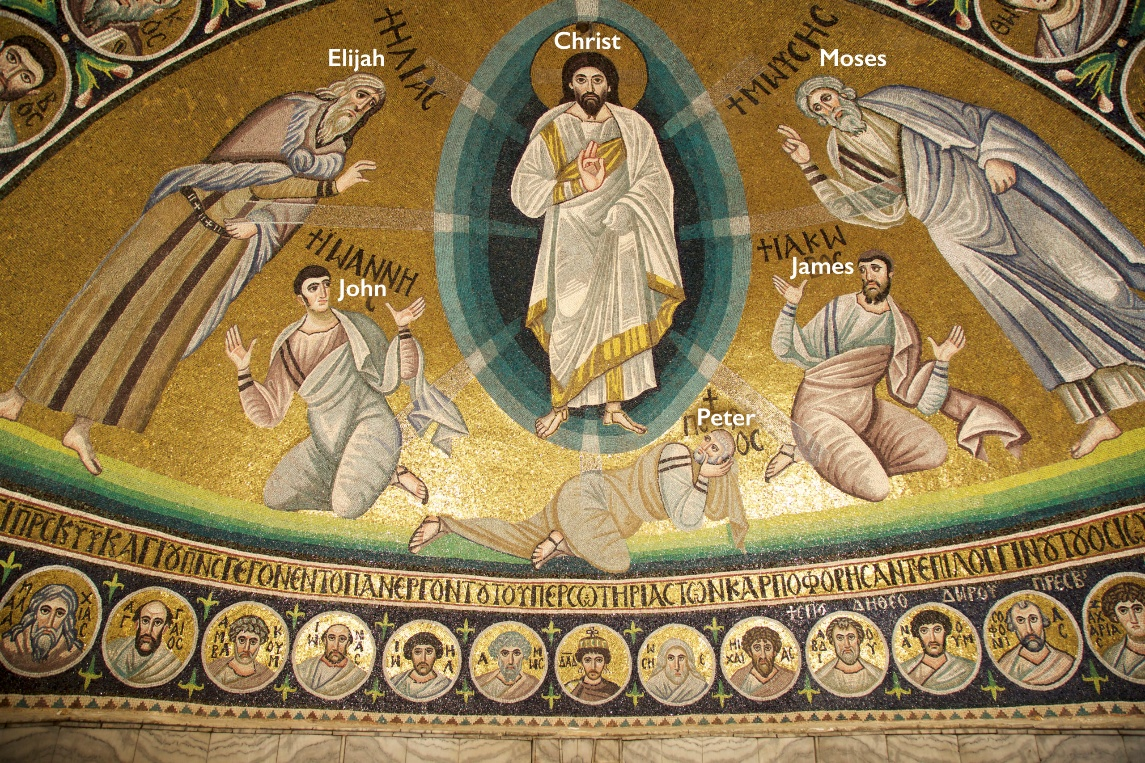
\includegraphics[width=0.85\linewidth]{image47.jpeg}
  \caption{Mosaico da Transfiguração no Mosteiro de Santa Catarina (século VI). Esta obra representa um dos mais antigos exemplos preservados da iconografia bizantina sobre temas escatológicos.}
  \label{fig:cap12-img8}
\end{figure}

Mosaico da Transfiguração no Mosteiro de Santa Catarina (século VI). Esta obra representa um dos mais antigos exemplos preservados da iconografia bizantina sobre temas escatológicos.

A teologia escatológica distinta dos Padres orientais manifestou-se não só em tratados e sermões, mas também de forma viva nas artes visuais e na literatura apocalíptica. Diversas formas de arte cristã oriental --- afrescos, ícones, mosaicos e iluminuras de manuscritos --- oferecem um testemunho pictórico das ideias sobre o céu, o inferno e a salvação. Nesta seção, exploramos algumas dessas representações escatológicas, que complementam e refletem a teologia desenvolvida nas tradições siríaca, copta, bizantina e outras.

Desde os primeiros séculos, circulavam entre os cristãos do Oriente textos apocalípticos que descreviam visões do além, muitas vezes acompanhados de ilustrações. Um exemplo antigo é o já mencionado Apocalipse de Pedro, cuja versão copta (preservada em fragmentos dos séculos VIII--IX encontrados em Akhmim, Egito) detalha cenas do inferno e do paraíso. Essas narrativas gráficas inspiraram a imaginação popular: nelas encontramos pecadores pendurados sobre abismos flamejantes, lagos de fogo e serpentes, assim como anjos misericordiosos intercedendo pelas almas --- imagens que influenciariam a iconografia posterior. Versões árabes medievais do mesmo Apocalipse de Pedro atestam a difusão dessas tradições no mundo cristão de língua árabe, atualizando a linguagem mas conservando os elementos essenciais das visões infernais e da esperança de salvação para alguns após a expiação.

Outro texto influente foi o Apocalipse de Paulo, que circulou em grego, siríaco, copta e outras línguas orientais. As versões siríacas dessa obra desenvolvem uma iconografia particular, muitas vezes ilustrada nos manuscritos: Paulo é conduzido por um anjo através de cenários celestiais e infernais, onde presencia tanto as delícias reservadas aos justos quanto os tormentos dos ímpios. Interessantemente, algumas variantes orientais do Apocalipse de Paulo inserem momentos em que os condenados obtêm alívio temporário de suas penas graças às orações dos santos --- reforçando, mais uma vez, o tema da misericórdia mesmo em contexto de punição. Os manuscritos iluminados desses apocalipses serviram como “Bíblias dos iletrados”, comunicando por meio de imagens fortes as verdades escatológicas ensinadas pela Igreja e complementando a catequese oral.


\begin{figure}[ht]
  \centering
  \includegraphics[width=0.85\linewidth]{image48.png}
  \caption{Fragmento do Apocalipse de Pedro de Akhmim (século VIII-IX). Este manuscrito copto preserva uma das mais antigas descrições cristãs detalhadas do inferno, incorporando elementos da tradição egípcia.}
  \label{fig:cap12-img9}
\end{figure}

Fragmento do Apocalipse de Pedro de Akhmim (século VIII-IX). Este manuscrito copto preserva uma das mais antigas descrições cristãs detalhadas do inferno, incorporando elementos da tradição egípcia.


\begin{figure}[ht]
  \centering
  \includegraphics[width=0.85\linewidth]{image49.png}
  \caption{Apocalipse Árabe de Pedro - Manuscrito medieval que demonstra a continuidade das tradições apocalípticas orientais e sua influência no mundo árabe-cristão.}
  \label{fig:cap12-img10}
\end{figure}

Apocalipse Árabe de Pedro - Manuscrito medieval que demonstra a continuidade das tradições apocalípticas orientais e sua influência no mundo árabe-cristão.

\subsection{Manuscritos Siríacos}


\begin{figure}[ht]
  \centering
  \includegraphics[width=0.85\linewidth]{image50.png}
  \caption{Manuscrito síríaco do Apocalipse de Paulo. As versões síríacas desenvolvem uma iconografia específica que enfatiza a misericórdia divina mesmo em contextos de punição.}
  \label{fig:cap12-img11}
\end{figure}

Manuscrito síríaco do Apocalipse de Paulo. As versões síríacas desenvolvem uma iconografia específica que enfatiza a misericórdia divina mesmo em contextos de punição.

Um dos temas iconográficos mais característicos da arte cristã oriental é a Anástasis, isto é, a Descida de Cristo aos Infernos após Sua crucificação, para libertar os justos do Antigo Testamento. Essa cena, virtualmente onipresente na arte bizantina e ortodoxa, encapsula a teologia da vitória de Cristo sobre a morte e Sua infinita misericórdia. Em magníficos afrescos, como o do Mosteiro de Chora em Constantinopla (início do século XIV), Cristo é representado rompendo as portas do inferno, que jazem despedaçadas sob Seus pés, e erguendo de suas tumbas Adão e Eva, juntamente com outros justos do passado. Não há imagem mais eloquente do triunfo da graça sobre a condenação: na Anástasis, o inferno aparece como um poder efêmero cujos cativos são libertos pelo Salvador.

Os detalhes desses ícones reforçam nuances teológicas importantes. Cristo é envolto em mandorla de luz --- a mesma luz divina incriada de que falam os hesicastas --- iluminando as cavernas sombrias do Hades. As figuras de Satanás e da Morte são mostradas acorrentadas ou subjugadas, indicando que o poder do mal foi derrotado não por meio de vingança, mas por um ato redentor de amor. Essa ênfase difere das representações ocidentais medievais, nas quais a descida de Cristo ao Limbo (um conceito correlato) é menos central. Na tradição oriental, pelo contrário, a Anástasis ocupa frequentemente o espaço principal nas decorações absidais das igrejas no ciclo pascal, lembrando os fiéis de que a Ressurreição de Cristo se estende a todos os tempos e lugares, resgatando até mesmo os mortos.


% (image51 removida por redundância com image62 — ambas representam o mesmo fresco
%  da Anastasis no Mosteiro de Chora, c. 1315; image62 é mantida como detalhe
%  subsequente na seção "A Tradição Bizantina da Anastasis".)

Paralelamente ao tema jubiloso da Anástasis, os artistas orientais também representaram cenas do Juízo Final e do inferno propriamente dito, embora com abordagens que refletem as sensibilidades teológicas locais. Nos mosaicos e afrescos bizantinos, Cristo é frequentemente retratado como Pantocrator (Soberano do Universo) em majestade, presidindo o Juízo Final. Sob Seu olhar, os justos são separados dos pecadores, mas mesmo nessa separação, a arte oriental tende a enfatizar a ordem cósmica e a misericórdia sobre o terror. Por exemplo, num célebre mosaico de Cristo Pantocrator na Catedral de Cefalù (séc. XII, na Sicília -- região então de influência bizantina), Cristo aparece com expressão serena e benevolente, rodeado pelos símbolos dos evangelistas e coros angelicais, diferindo do semblante severo que se veria em alguns afrescos góticos ocidentais.

Nas representações especificamente do inferno, as igrejas bizantinas costumam relegá-lo a uma parte inferior ou lateral da composição do Juízo. O inferno aparece como uma região de trevas, fora da presença de Deus, por vezes figurado como um abismo negro ou a boca de um monstro (remetendo à figura bíblica de Leviatã devorando os réprobos). Em afrescos como os da igreja de Panagia Asinou, em Chipre (séculos XI--XII), vê-se um rio de fogo saindo do trono de Cristo (uma imagem tomada do livro do Apocalipse e da profecia de Daniel) que desce até esse abismo onde almas padecem.

Os demônios são pintados atormentando os condenados, mas sem o deleite macabro que se nota em miniaturas medievais ocidentais; ao contrário, sua imagem transmite a execução da justiça divina sob o limite imposto pela soberania de Deus. Anjos frequentemente estão presentes na cena, indicando que até mesmo o castigo ocorre sob a permissão e controle divinos. Essa iconografia traz implícita a ideia de que a justiça de Deus nunca está desvinculada de Sua misericórdia.

Nos Bálcãs e em territórios eslavos sob influência bizantina, surgiram variações locais interessantes. No Mosteiro de São Joaquim de Osogovo (Macedônia), um afresco do inferno mostra demônios encadeando os pecadores, mas inclui também, na mesma composição, a cena do Sábado Santo (Cristo descendo ao Hades) ao lado, insinuando que a condenação não é a última palavra. De modo geral, nas igrejas ortodoxas, a cena do inferno é integrada à visão ampla do Juízo Final --- o que comunica visualmente que, embora haja condenados, eles permanecem parte do panorama maior do plano divino, no qual a justiça é temperada pela esperança.


\begin{figure}[ht]
  \centering
  \includegraphics[width=0.85\linewidth]{image52.jpeg}
  \caption{Afresco representando o inferno na Igreja Panagia Asinou, Chipre (século XI-XII). As representações bizantinas mostram o inferno como região de escuridão e separação de Deus.}
  \label{fig:cap12-img13}
\end{figure}

Afresco representando o inferno na Igreja Panagia Asinou, Chipre (século XI-XII). As representações bizantinas mostram o inferno como região de escuridão e separação de Deus.


\begin{figure}[ht]
  \centering
  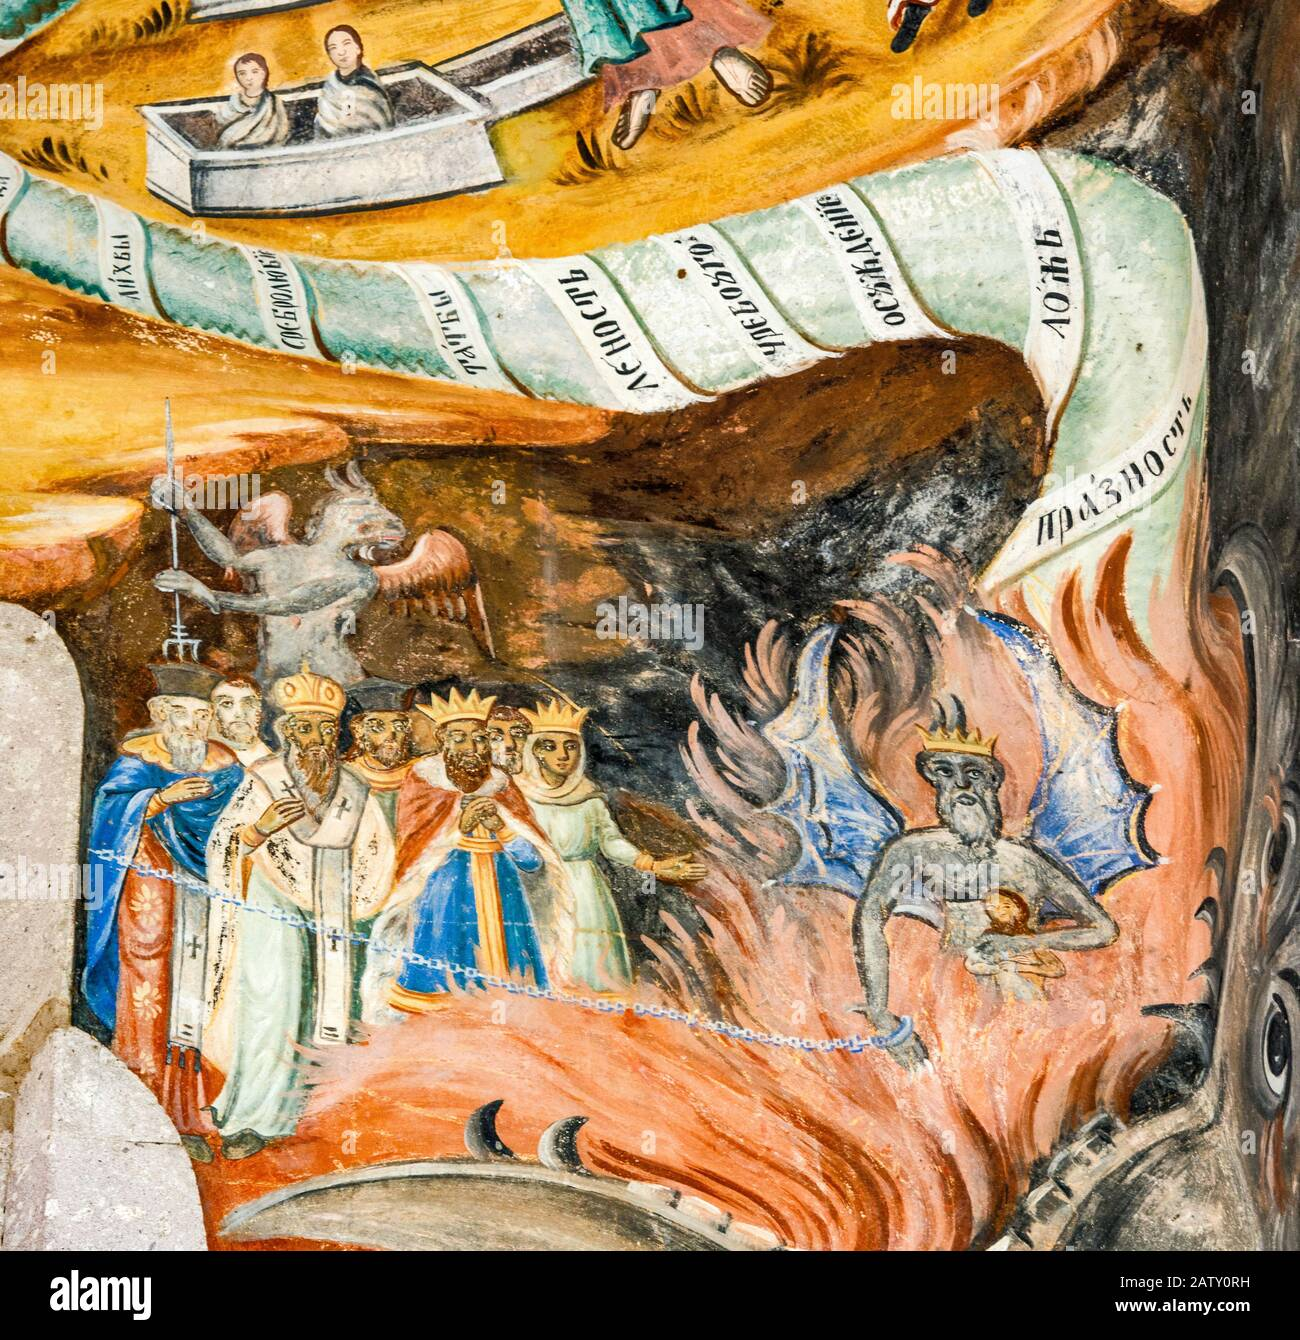
\includegraphics[width=0.85\linewidth]{image53.jpeg}
  \caption{Afresco do inferno na Igreja de São Joaquim de Osogovo, com demônios e almas em tormento no cenário do Juízo.}
  \label{fig:cap12-img14}
\end{figure}

Afresco do inferno na Igreja de São Joaquim de Osogovo, Mosteiro Ortodoxo Macedônio. Demônios e almas em tormento são representados dentro de um contexto que enfatiza a justiça temperada pela misericórdia.

As tradições armênia e copta, já mencionadas em termos teológicos, legaram também interpretações visuais únicas de temas escatológicos. A arte armênia medieval, especialmente nos séculos XIII--XIV, produziu manuscritos ricamente iluminados que retratam cenas do Juízo Final e da descida de Cristo ao Inferno com um estilo próprio. O miniaturista armênio Sargis Pitsak, por exemplo, ilustrou em 1346 uma Crucifixão na qual, ao pé da cruz, há uma sugestão do mundo subterrâneo e da derrota do demônio, combinando a teologia da cruz com a da vitória de Cristo sobre o Hades. Em outros fólios armênios, como no famoso manuscrito de Homilias de Mock‘ats‘i (séc. XIII) ou em páginas do Himnário de Zeytun (séc. XV), Cristo é mostrado puxando Adão e outros justos da boca de um monstro infernal em composições derivadas da Anástasis bizantina, porém incorporando cores mais vibrantes e figuras com traços próprios da cultura local.

A iconografia copta, por sua vez, continuou a refletir a fusão com símbolos faraônicos. Em algumas igrejas coptas medievais encontram-se pinturas do Arcanjo Miguel segurando uma balança a pesar as almas --- um claro paralelo cristianizado da psicostasia (pesagem do coração) do Livro dos Mortos egípcio. Numa dessas representações, enquanto Miguel pesa o coração do falecido contra a Palavra de Deus (ou contra uma pena simbolizando a Verdade), um demônio tenta furtivamente manipular o resultado, mas é repelido pelo poder divino, ressaltando a justiça final incorruptível.

Essa imagem resume bem a integração cultural realizada: um conceito pagão egípcio é reaproveitado para ensinar a necessidade de pureza de coração perante o julgamento de Cristo. Além disso, tradições populares coptas desenvolveram narrativas em que santos visitam o inferno e o paraíso guiados por anjos (similares às jornadas visionárias de Paulo e Pedro), descritas em textos como o Apocalipse de Samuel de Kalamoun (século X) e acompanhadas de ícones vivos. Essas obras tinham tanto um propósito catequético quanto devocional, educando os fiéis iletrados e reforçando a realidade do Juízo Final de uma forma sensível à imaginação cultural egípcia.

Iluminura armênia medieval (Matenadaran, Yerevan) representando a Descida de Cristo ao Inferno. A composição combina elementos bizantinos com características iconográficas localmente desenvolvidas.

Fólio de manuscrito armênio mostrando Cristo descendo ao Inferno para libertar as almas. Elementos de tradições pré-cristãs locais são adaptados a um contexto cristão nessa representação.

Representação copta da “pesagem do coração” (psicostasia) adaptando o conceito faraônico de julgamento pós-morte. Ilustra como os coptas integraram tradições religiosas egípcias antigas à teologia cristã.

\subsection{Ícones Ortodoxos Pós-Bizantinos do Juízo Final}

Após a queda de Constantinopla (1453), a tradição bizantina continuou viva nos territórios ortodoxos e foi gradualmente enriquecida por novos elementos. Ícones do Juízo Final produzidos na escola cretense de pintura (séculos XVI--XVII), por exemplo, combinam a herança bizantina com influências do Renascimento ocidental. Obras de mestres como Franghias Kavertzas e Georgios Klontzas retratam o cenário completo do Juízo: Cristo entronizado, anjos abrindo os livros, a Virgem Maria e João Batista intercedendo (a composição da Deesis), os apóstolos julgando as nações, os justos guiados ao céu e os pecadores arrastados ao inferno.

Nesses ícones, o inferno ocupa a parte inferior ou lateral da cena, exibindo níveis distintos de punição para diferentes tipos de pecados. Esse detalhamento ecoa as visões apocalípticas medievais, embora reinterpretado pelos artistas ortodoxos. Entretanto, mesmo com tais elementos dramáticos, a figura de Cristo permanece central e dominante, assegurando que o foco narrativo seja o triunfo final de Deus, e não as angústias infernais em si.

Um detalhe frequente nos ícones pós-bizantinos é a presença de inscrições ou poemas explicativos que enfatizam o aspecto moral e espiritual das cenas. Por exemplo, junto às figuras de condenados podem aparecer trechos litúrgicos lembrando que “Deus os chamou, mas eles não quiseram ouvir”. Isso reforça a interpretação de que a condenação é fruto da obstinação humana, não de falta de misericórdia divina. Ademais, esses ícones eram muitas vezes encomendados por mosteiros, cujos monges patronos zelavam pela ortodoxia do conteúdo teológico representado: imagens excessivamente cruas ou desesperançosas eram evitadas, preservando-se o equilíbrio entre justiça e misericórdia.

Por fim, vale notar que os mosteiros ortodoxos atuaram como verdadeiros museus vivos dessa iconografia escatológica. Ao viajar pelos Bálcãs ou pelo Oriente Médio, ainda hoje se podem admirar, em antigas igrejas monásticas, afrescos do céu e do inferno lado a lado. Esses lugares sagrados mantiveram acesa a chama da visão patrística oriental: o inferno representado não como simples instrumento de terror, mas como parte de uma pedagogia divina que, sem negar a realidade da pena eterna, convida constantemente à metanoia (mudança de mente e coração) e à busca da união com Deus.


\begin{figure}[ht]
  \centering
  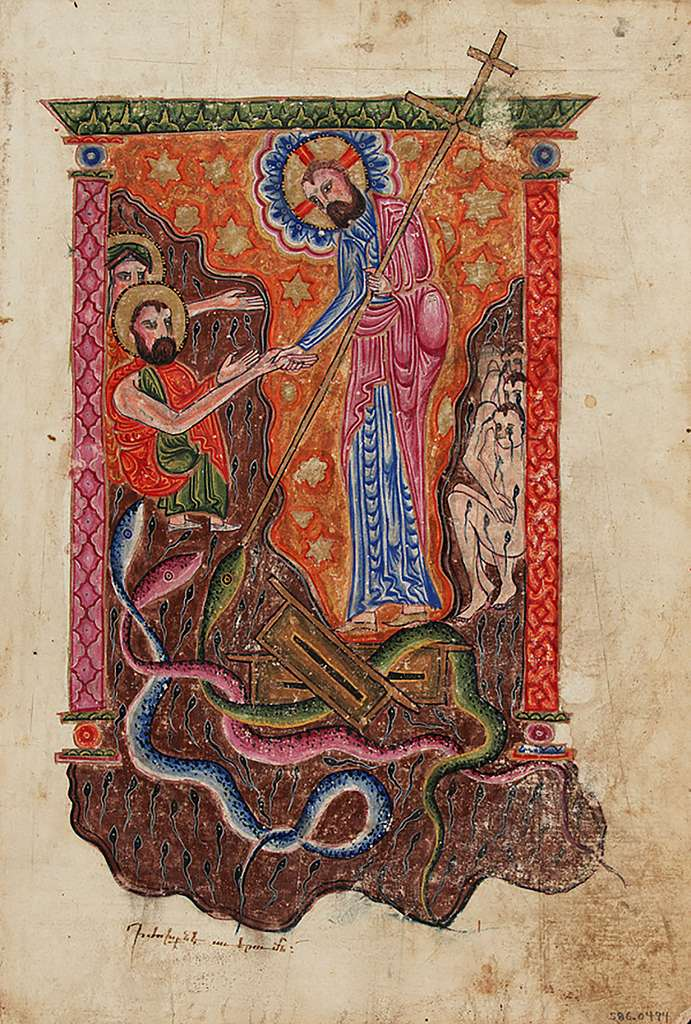
\includegraphics[width=0.85\linewidth]{image54.jpeg}
  \caption{Jesus Desce ao Inferno - Fólio de manuscrito armênio mostrando Cristo libertando as almas, incorporando elementos de tradições locais pré-cristãs adaptados ao contexto cristão.}
  \label{fig:cap12-img15}
\end{figure}

Jesus Desce ao Inferno - Fólio de manuscrito armênio mostrando Cristo libertando as almas, incorporando elementos de tradições locais pré-cristãs adaptados ao contexto cristão.


\begin{figure}[ht]
  \centering
  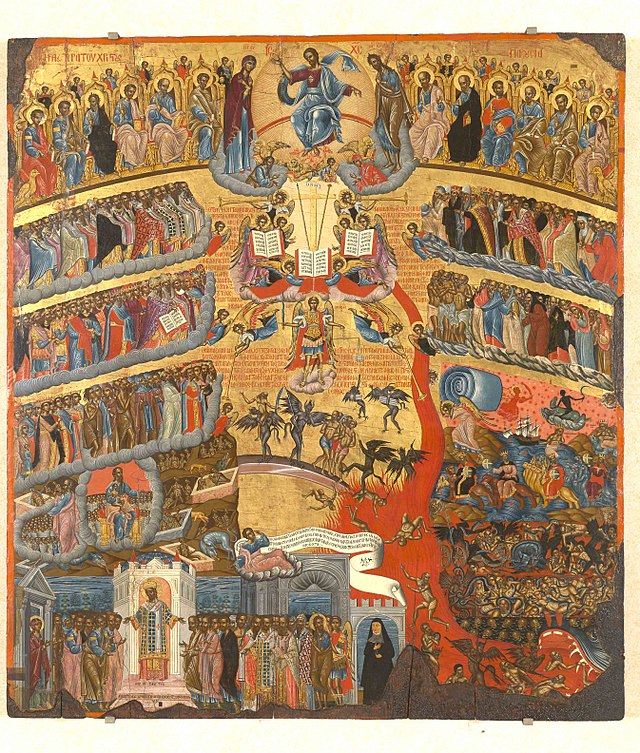
\includegraphics[width=0.85\linewidth]{image55.jpeg}
  \caption{Juízo Final por F. Kavertzas (1640-41). As representações ortodoxas incluem o inferno como parte de uma composição que enfatiza tanto a justiça quanto a misericórdia divina.}
  \label{fig:cap12-img16}
\end{figure}

Juízo Final por F. Kavertzas (1640-41). As representações ortodoxas incluem o inferno como parte de uma composição que enfatiza tanto a justiça quanto a misericórdia divina.


\begin{figure}[ht]
  \centering
  \includegraphics[width=0.85\linewidth]{image56.png}
  \caption{Detalhe do inferno no \emph{Juízo Final} de Georgios Klontzas, final do século XVI, organizado em diferentes níveis de punição.}
  \label{fig:cap12-img17}
\end{figure}

Detalhe do inferno no Juízo Final por Georgios Klontzas (final do século XVI). Mostra diferentes níveis de punição, refletindo influências de tradições patrísticas orientais e desenvolvimentos teológicos posteriores.

Os Padres da Igreja orientais apresentaram uma abordagem singular à escatologia cristã, marcada pelo equilíbrio entre a justiça divina e a esperança misericordiosa de redenção. Desde os poéticos hinos siríacos de Efrém até as visões místicas dos hesicastas bizantinos, passando pelas adaptações culturais de coptas, armênios e georgianos, emergiu uma ênfase comum na transformação interior e na deificação como finalidade última da alma. Em contraste com certas tendências ocidentais que, em períodos medievais, acentuaram o aspecto estritamente jurídico do juízo divino, a tradição oriental jamais perdeu de vista o caráter medicinal e pedagógico dos castigos de Deus: o inferno, em última instância, é entendido como a experiência da ausência de Deus por parte de quem rejeita Seu amor, e não meramente um castigo externo imposto de fora.

Essa rica herança teológica refletiu-se nas artes sacras e sobreviveu através dos séculos nas liturgias e mosteiros do Oriente. Para o estudioso contemporâneo, ela oferece perspectivas valiosas --- e por vezes esquecidas --- de um Cristianismo antigo que soube harmonizar temor e esperança. Ao destacar a misericórdia e a possibilidade de metanoia (arrependimento transformador), mesmo diante das realidades últimas, os Padres orientais legaram uma visão escatológica profundamente espiritual e compassiva. Tal visão continua a inspirar o pensamento teológico e a iconografia da Igreja até os dias de hoje, lembrando-nos de que, na economia divina, a justiça está sempre entrelaçada com a graça.

\section{Os Desenvolvimentos Patrísticos Orientais: Uma Tradição Teológica Distintiva}


Os desenvolvimentos patrísticos orientais representam uma tradição teológica distintiva que oferece perspectivas únicas sobre escatologia e punição eterna, frequentemente contrastando com sínteses latinas contemporâneas. Esta tradição, florescendo nas culturas siríaca, copta, bizantina e armênia, desenvolve teologias sofisticadas que integram elementos de filosofia grega, tradições semíticas orientais e experiência mística, criando sínteses escatológicas que enfatizam transformação ao invés de punição retributiva.

\subsection{Tradições Siríacas e a Teologia Poética de Efrém}


% (image57 removida: ícone moderno de Santo Efrém redundante com image40
%  (mosaico histórico, c. XI, Mosteiro de Nea Moni). Mantida a versão
%  histórica como evidência iconográfica mais antiga da tradição siríaca.)

As tradições siríacas, particularmente através da Escola de Edessa e figuras como Efrém, o Sírio (306-373), desenvolvem teologia poética que incorpora imagery paradisíaca e infernal em hinos e homilias que influenciam profundamente espiritualidade popular oriental. Os Hinos sobre o Paraíso de Efrém apresentam geografia escatológica que contrasta paraíso estratificado com regiões de punição, mas enfatiza misericórdia divina e possibilidade de intercessão pelos mortos. Esta ênfase em compaixão divina distingue desenvolvimentos siríacos de ênfases latinas contemporâneas em justiça retributiva.

\subsection{A Tradição Copta e suas Influências Egípcias}


A tradição copta, desenvolvida no contexto do cristianismo egípcio, incorpora elementos significativos de tradições faraônicas sobre julgamento pós-morte adaptados a conceitos cristãos. Textos como o Apocalipse copto de Pedro e a Literatura de Shenute de Atripe (348-465) desenvolvem descrições detalhadas de tormentos infernais que incorporam elementos de iconografia egípcia tradicional. A influência monástica de figuras como Antão do Egito (251-356) e Pacômio (292-348) introduz elementos de experiência ascética que transformam conceitos escatológicos em realidades experienciais antecipadas através de práticas contemplativas.


\section{Teologia Bizantina: Sínteses Sofisticadas}




São Máximo, o Confessor (580-662) - Ícone da Igreja Ortodoxa Americana. Sua doutrina sobre os logoi divinos ofereceu um framework teológico onde a punição eterna representa resistência ao movimento natural da alma.

A teologia bizantina, culminando em figuras como Máximo o Confessor (580-662) e João Damasceno (676-749), desenvolve sofisticadas sínteses que incorporam elementos de teologia capadócia com inovações próprias sobre theosis (deificação) e escatologia. A doutrina maximiana sobre logoi divinos e movimento natural da criação em direção a Deus oferece framework teológico onde punição eterna representa resistência ao movimento natural da alma em direção à sua finalidade divina, ao invés de imposição externa de sofrimento.

\subsection{A Tradição Hesiquiasta e a Experiência Mística}

O desenvolvimento da teologia hesiquiasta (sécs. IV-XIV) através de figuras como Evágrio Pôntico (345-399), João Clímaco (579-649), e Gregório Palamas (1296-1359) introduz dimensão experiencial na escatologia através de práticas contemplativas que antecipam estados pós-morte. A doutrina palamita sobre energias divinas não-criadas oferece explicação teológica para experiências místicas de luz divina que contrasta com escuridão infernal, criando economia escatológica baseada em participação ao invés de retribuição legal.

\subsection{Tradições Armênia e Georgiana}


\begin{figure}[ht]
  \centering
  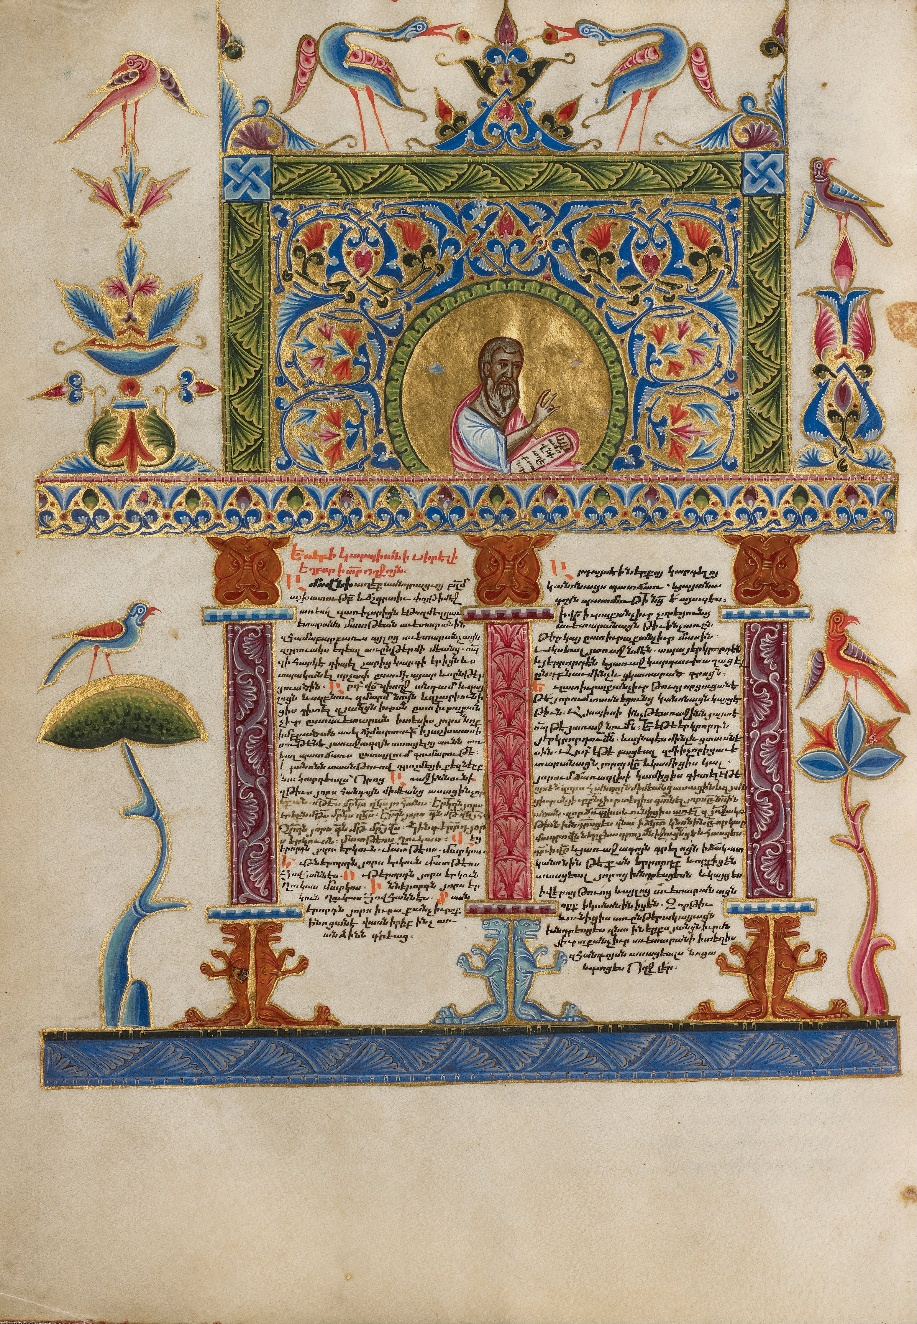
\includegraphics[width=0.85\linewidth]{image58.jpeg}
  \caption{Página decorada de manuscrito armênio iluminado. Os manuscritos armênios desenvolveram uma tradição iconográfica única que combina elementos bizantinos com características distintamente locais.}
  \label{fig:cap12-img24}
\end{figure}

Página decorada de manuscrito armênio iluminado. Os manuscritos armênios desenvolveram uma tradição iconográfica única que combina elementos bizantinos com características distintamente locais.


\begin{figure}[ht]
  \centering
  \includegraphics[width=0.85\linewidth]{image59.jpeg}
  \caption{Crucifixão de Jesus por Sargis Pitsak (1346) - Exemplo da arte armênia medieval que adapta conceitos escatológicos gregos a contextos culturais específicos.}
  \label{fig:cap12-img25}
\end{figure}

Crucifixão de Jesus por Sargis Pitsak (1346) - Exemplo da arte armênia medieval que adapta conceitos escatológicos gregos a contextos culturais específicos.

As tradições armênia e georgiana desenvolvem sínteses únicas que incorporam elementos de tradições locais pré-cristãs com teologia bizantina. Textos como a História de Agathangelos e os escritos de Eznik de Kolb (c. 380-450) apresentam adaptações de conceitos escatológicos gregos a contextos culturais específicos, criando tradições nacionais distintivas que persistem até o presente.

\section{Iconografia Oriental e Representação Escatológica}


\begin{figure}[ht]
  \centering
  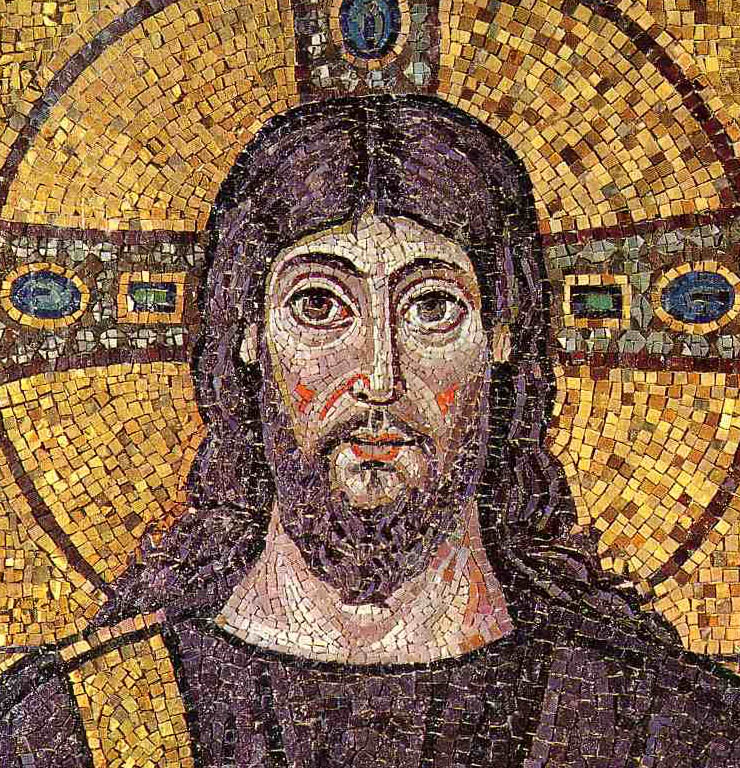
\includegraphics[width=0.85\linewidth]{image60.jpeg}
  \caption{Cristo Pantocrator - Mosaico bizantino de Ravenna. As representações orientais enfatizam a majestade divina ao invés da severidade punitiva, refletindo ênfases teológicas em theosis e misericórdia.}
  \label{fig:cap12-img26}
\end{figure}

Cristo Pantocrator - Mosaico bizantino de Ravenna. As representações orientais enfatizam a majestade divina ao invés da severidade punitiva, refletindo ênfases teológicas em theosis e misericórdia.


\begin{figure}[ht]
  \centering
  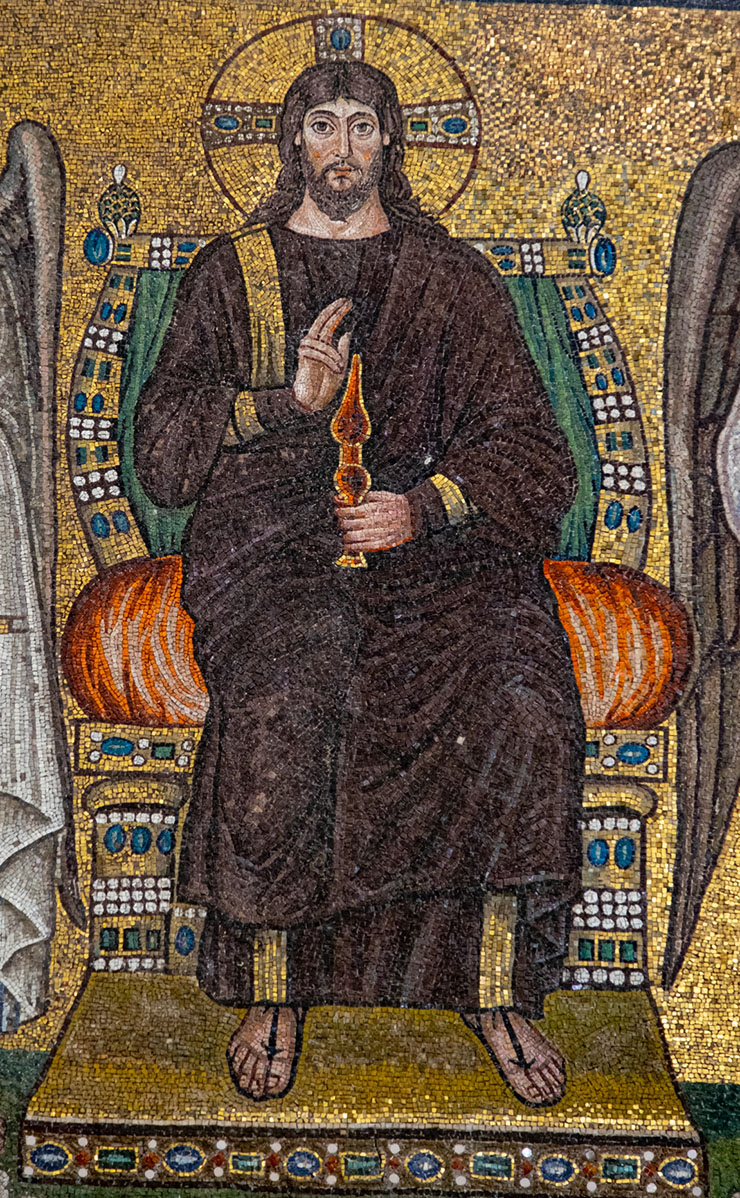
\includegraphics[width=0.85\linewidth]{image61.jpeg}
  \caption{Mosaicos bizantinos de Ravenna demonstrando a tradição iconográfica oriental que apresenta Cristo em contextos de julgamento final com ênfase na majestade divina.}
  \label{fig:cap12-img27}
\end{figure}

Mosaicos bizantinos de Ravenna demonstrando a tradição iconográfica oriental que apresenta Cristo em contextos de julgamento final com ênfase na majestade divina.

A iconografia oriental desenvolve tradições visuais específicas de representação escatológica que diferem significativamente de desenvolvimentos ocidentais. Mosaicos bizantinos como os de Ravenna e Constantinopla apresentam Christ Pantocrator em contextos de julgamento final que enfatizam majestade divina ao invés de severidade punitiva, refletindo ênfases teológicas orientais em theosis e misericórdia divina.

\section{Impacto das Invasões Islâmicas}

O impacto das invasões islâmicas (séc. VII em diante) sobre desenvolvimentos patrísticos orientais cria contextos de diálogo inter-religioso que influenciam conceitos escatológicos. Figuras como João Damasceno, vivendo sob domínio islâmico, desenvolvem apologética que necessariamente engaja com conceitos islâmicos sobre paraíso e inferno, criando sínteses que incorporam elementos de ambas tradições.

A preservação de tradições patrísticas orientais em monastérios como Monte Athos, Mosteiro de Santa Catarina (Sinai), e centros coptos no Egito assegura continuidade cultural destas tradições através de períodos de turbulência política. Esta continuidade permite desenvolvimento orgânico de teologias escatológicas orientais que mantêm características distintivas face a influências ocidentais posteriores.

\section{Representações do Inferno na Arte Patrística Oriental}

\section{Tradições Manuscritas e Apocalípticas}

\subsection{O Apocalipse Copto de Pedro}


\subsection{Manuscritos Siríacos}


\section{A Tradição Bizantina da Anastasis}

\subsection{O \emph{Harrowing of Hell} nos Afrescos Bizantinos}


\begin{figure}[ht]
  \centering
  \includegraphics[width=0.85\linewidth]{image62.jpeg}
  \caption{Detalhe da Anastasis mostrando Cristo libertando as almas do limbo. Esta iconografia enfatiza o triunfo sobre a morte ao invés do castigo eterno, característica distintiva da teologia oriental.}
  \label{fig:cap12-img32}
\end{figure}

Detalhe da Anastasis mostrando Cristo libertando as almas do limbo. Esta iconografia enfatiza o triunfo sobre a morte ao invés do castigo eterno, característica distintiva da teologia oriental.

\subsection{Características da Representação Bizantina}




Afresco do inferno na Igreja de São Joaquim de Osogovo, Mosteiro Ortodoxo Macedônio. Demônios e almas em tormento são representados dentro de um contexto que enfatiza a justiça temperada pela misericórdia.

\section{Tradições Armênias e Manuscritos Iluminados}


\begin{figure}[ht]
  \centering
  \includegraphics[width=0.85\linewidth]{image63.jpeg}
  \caption{Versão copta da pesagem do coração - Adaptação cristã do conceito faraônico de julgamento pós-morte. Mostra como as comunidades coptas integraram tradições egípcias ancestrais com teologia cristã.}
  \label{fig:cap12-img36}
\end{figure}

Versão copta da pesagem do coração - Adaptação cristã do conceito faraônico de julgamento pós-morte. Mostra como as comunidades coptas integraram tradições egípcias ancestrais com teologia cristã.

\section{O Juízo Final na Iconografia Ortodoxa}




Detalhe do inferno no Juízo Final por Georgios Klontzas (final do século XVI). Mostra diferentes níveis de punição, refletindo influências de tradições patrísticas orientais e desenvolvimentos teológicos posteriores.


\begin{figure}[ht]
  \centering
  \includegraphics[width=0.85\linewidth]{image64.jpeg}
  \caption{Afresco ortodoxo mostrando representações do céu e inferno com figuras humanas em cenas do Juízo Final. Demonstra a tradição oriental de inserir estas imagens em programas iconográficos mais amplos.}
  \label{fig:cap12-img39}
\end{figure}

Afresco ortodoxo mostrando representações do céu e inferno com figuras humanas em cenas do Juízo Final. Demonstra a tradição oriental de inserir estas imagens em programas iconográficos mais amplos.


\begin{figure}[ht]
  \centering
  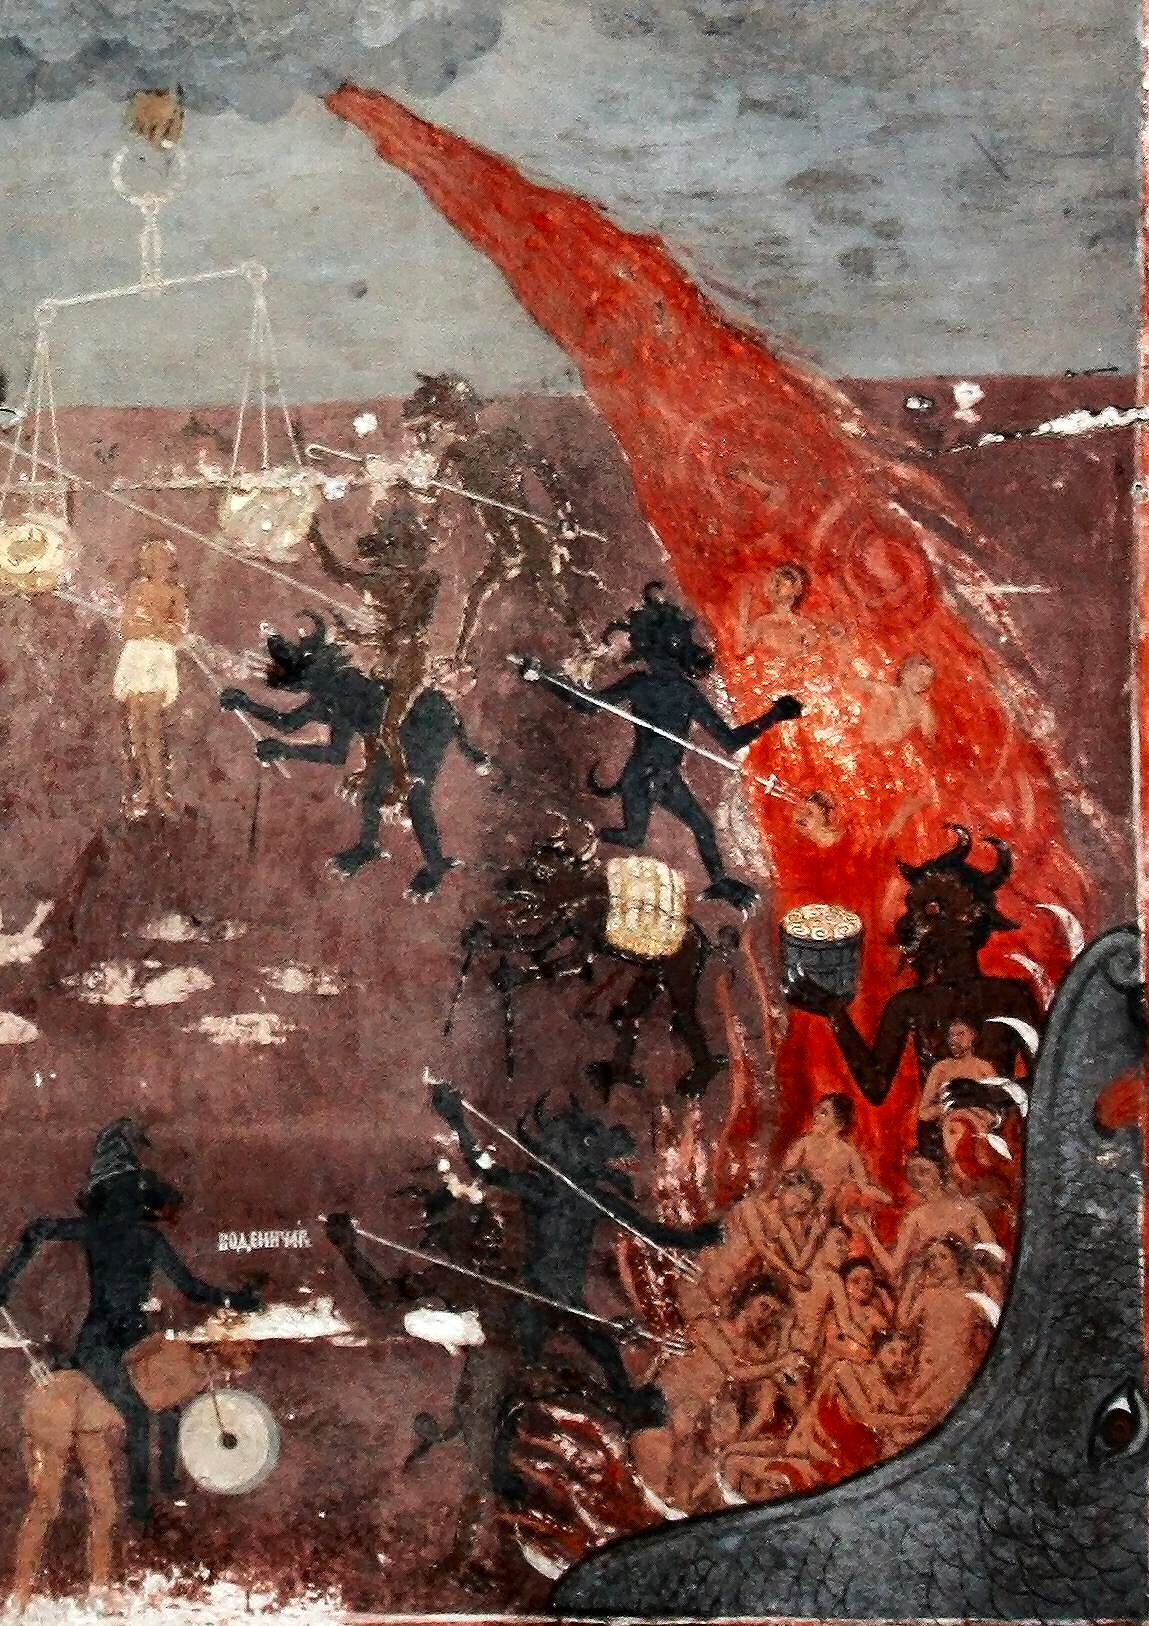
\includegraphics[width=0.85\linewidth]{image65.jpeg}
  \caption{Afresco do inferno no Mosteiro de Raduil, Bulgária, testemunho da continuidade da iconografia escatológica ortodoxa.}
  \label{fig:cap12-img40}
\end{figure}

Afresco do inferno do Mosteiro de Raduil, Bulgária. A preservação dessas tradições em contextos monásticos assegurou a continuidade de uma tradição visual que reflete as ênfases teológicas orientais em theosis e economia divina.

% ============================================================
% PARTE IV: SÍNTESES MEDIEVAIS E MODERNAS
% ============================================================

\part{SÍNTESES MEDIEVAIS E MODERNAS}
\partmark{SÍNTESES MEDIEVAIS E MODERNAS}

% --- Capítulo 13: Influências Islâmicas no Cristianismo Medieval ---
\chapter[Influências Islâmicas]{Influências Islâmicas no Cristianismo Medieval}


\epigraph{O Islã apresenta uma escatologia ricamente detalhada, do Mi‘rāj do Profeta aos sete portões de Jahannam --- um imaginário que dialogou profundamente com as visões cristãs medievais, da Visão de Túndalo à síntese dantesca.}

Escatologia Islâmica Normativa: Paraíso, Inferno, Julgamento e Ressurreição

No Islã, a crença na vida após a morte (al-ākhirah) é um dos seis artigos de fé fundamentais en.wikipedia.org. A perspectiva escatológica islâmica, baseada no Alcorão e nos hadiths, afirma que a vida terrena é um teste passageiro que prepara cada alma para o destino eterno após a morte en.wikipedia.org. Após o término da vida mundana, Deus ressuscitará todos os seres humanos no Dia do Julgamento (Yawm al-Qiyāmah) para prestação de contas de suas obras. Nessa ressureição corporal, cada indivíduo terá seus feitos pesados na balança (al-mīzān) e receberá uma sentença justa: paraíso ou inferno, de acordo com seus méritos e faltas en.wikipedia.org.

A doutrina sunita clássica ensina que tanto o Paraíso (Jannah) quanto o Inferno (Jahannam) já foram criados por Deus e existem atualmente, embora sejam plenamente usufruídos apenas após o Juízo Final en.wikipedia.org. As fontes canônicas descrevem vividamente esses destinos. O Paraíso é representado como jardins sob os quais correm rios, com abundância de sombras, frutos e bem-aventuranças, onde os justos desfrutam de delícias físicas e espirituais eternas, inclusive a visão beatífica de Deus (segundo a maioria dos teólogos) en.wikipedia.org. Há referência a diferentes graus de Paraíso -- frequentemente enumerados em sete níveis -- sendo o mais elevado o Jannat al-Firdaus (Paraíso do Éden), reservado aos profetas e aos mais virtuosos. Igualmente, o Inferno é descrito com vários níveis ou “portões” (até sete) de tormento, cada qual apropriado a tipos de pecados en.wikipedia.org. O Alcorão alude, por exemplo, aos “sete portões” do inferno (Qur. 15:44), e tradições posteriores atribuem nomes específicos a cada estágio de Jahannam e seus castigos correspondentes. Em contraste com o prazer eterno do Paraíso, o Inferno é fogo devorador, sofrimento físico e remorso espiritual para os ímpios -- destino este considerado perpétuo pela ortodoxia (embora escolas teológicas clássicas tenham debatido a possibilidade de eventual misericórdia divina aos condenados) en.wikipedia.org.


\begin{figure}[ht]
 \centering
 \includegraphics[width=0.85\linewidth]{image66.jpeg}
 \caption{Ilustração 1 do capítulo.}
 \label{fig:cap13-img1}
\end{figure}

Miniatura persa do século XV mostrando Muhammad visitando o Paraíso (Jannah). A imagem retrata os jardins sob os quais correm rios, conforme descrito no Alcorão, com árvores frondosas, arquitetura celestial e figuras angelicais, ilustrando a visão islâmica do paraíso como lugar de delícias físicas e espirituais eternas. (Biblioteca Nacional da França, Supplément Persan 1030)


\begin{figure}[ht]
 \centering
 \includegraphics[width=0.85\linewidth]{image67.jpeg}
 \caption{- A Ascensão do Profeta}
 \label{fig:cap13-img2}
\end{figure}

O processo escatológico islâmico inclui também elementos como a Barzakh, etapa intermediária entre a morte e a ressurreição. Ao morrer, a alma do indivíduo entra nesse estado transitório no qual aguardará o Dia Final en.wikipedia.org. Nesse ínterim, ocorrem eventos como a visita dos anjos Munkar e Nakīr, que interrogam o falecido sobre sua fé; os crentes fiéis experimentam paz e os perversos já então sofrem tormentos precursores en.wikipedia.org. No Dia do Juízo, conforme os hadiths, todas as almas serão reunidas e julgadas diretamente por Deus, passando por cenas dramáticas: os registros de feitos serão abertos, as ações pesadas, e todos atravessarão a ponte sirāt (fina como lâmina sobre o abismo do inferno) rumo ao seu destino final. Os justos atravessam ilesos para a salvação, enquanto os condenados caem da ponte em direção ao fogo infernal, a menos que sejam resgatados por alguma intercessão divina. De fato, uma particularidade da escatologia islâmica é o papel da intercessão profética: o Profeta Muhammad -- assim como outros mensageiros e santos -- recebeu de Deus a prerrogativa de interceder em favor dos crentes pecadores no Dia Final en.wikipedia.org. Essa intercessão, segundo a doutrina sunita, permitirá que muitos muçulmanos que tenham cometido faltas graves acabem por serem perdoados e libertos do Inferno após cumprirem parte da pena en.wikipedia.org. Em última instância, portanto, Paraíso e Inferno são concebidos como moradas eternas e reais: o Jannah como prêmio imortal para os virtuosos e crentes, e o Jahannam como punição interminável para os descrentes e injustos en.wikipedia.org. A justiça perfeita de Deus se reflete nessa dicotomia, reforçando a responsabilidade moral individual e a necessidade de se viver conforme a orientação divina para assegurar um destino feliz no além en.wikipedia.org.

Paralelamente à escatologia “externa” normativa, desenvolveu-se dentro do Islã uma rica interpretação mística do pós-vida, sobretudo nas tradições do Sufismo (ta\d{s}awwuf). Os mestres sufis enfatizaram que a jornada para o além começa já nesta vida, por meio da purificação interior da alma (tazkiyat al-nafs) e da ascensão gradual por estágios espirituais (maqāmāt) em direção a Deus patheos.com. Em lugar de focar apenas em descrições literais de Paraíso e Inferno como lugares físicos, os sufis frequentemente interpretam essas realidades de maneira alegórica e interiorizada. Autores místicos tardios, como Ibn ‘Arabī (mestre andaluz do século XIII) e Jalāl ad-Dīn Rumi (poeta persa do século XIII), enfatizaram que o verdadeiro Paraíso é a proximidade de Deus e o verdadeiro Inferno é a distância ou separação d’Ele, estados esses que correspondem a condições da alma en.wikipedia.org. Assim, “o fogo do inferno nada mais é que o estado de consciência das próprias falhas como ser humano” -- um tormento auto-infligido pela percepção da distância do Real --, enquanto o deleite celestial é a realização íntima do Divino en.wikipedia.org. Para muitos sufis, as imagens corânicas de rios, jardins e hurīs no Paraíso, ou de chamas e torturas no Inferno, são símbolos de júbilo ou agonia espiritual que a alma experimenta conforme sua proximidade ou véus em relação a Deus en.wikipedia.org.

\begin{itemize}
 \item A Ascensão do Profeta
\end{itemize}

\begin{figure}[ht]
 \centering
 \includegraphics[width=0.85\linewidth]{image68.jpeg}
 \caption{4. Dia do Juízo Final (Yawm al-Qiyamah)}
 \label{fig:cap13-img3}
\end{figure}


\begin{figure}[ht]
 \centering
 \includegraphics[width=0.85\linewidth]{image69.jpeg}
 \caption{4. Dia do Juízo Final (Yawm al-Qiyamah)}
 \label{fig:cap13-img4}
\end{figure}

4. Dia do Juízo Final (Yawm al-Qiyamah)


\begin{figure}[ht]
 \centering
 \includegraphics[width=0.85\linewidth]{image70.jpeg}
 \caption{Ilustração 5 do capítulo.}
 \label{fig:cap13-img5}
\end{figure}


\begin{figure}[ht]
 \centering
 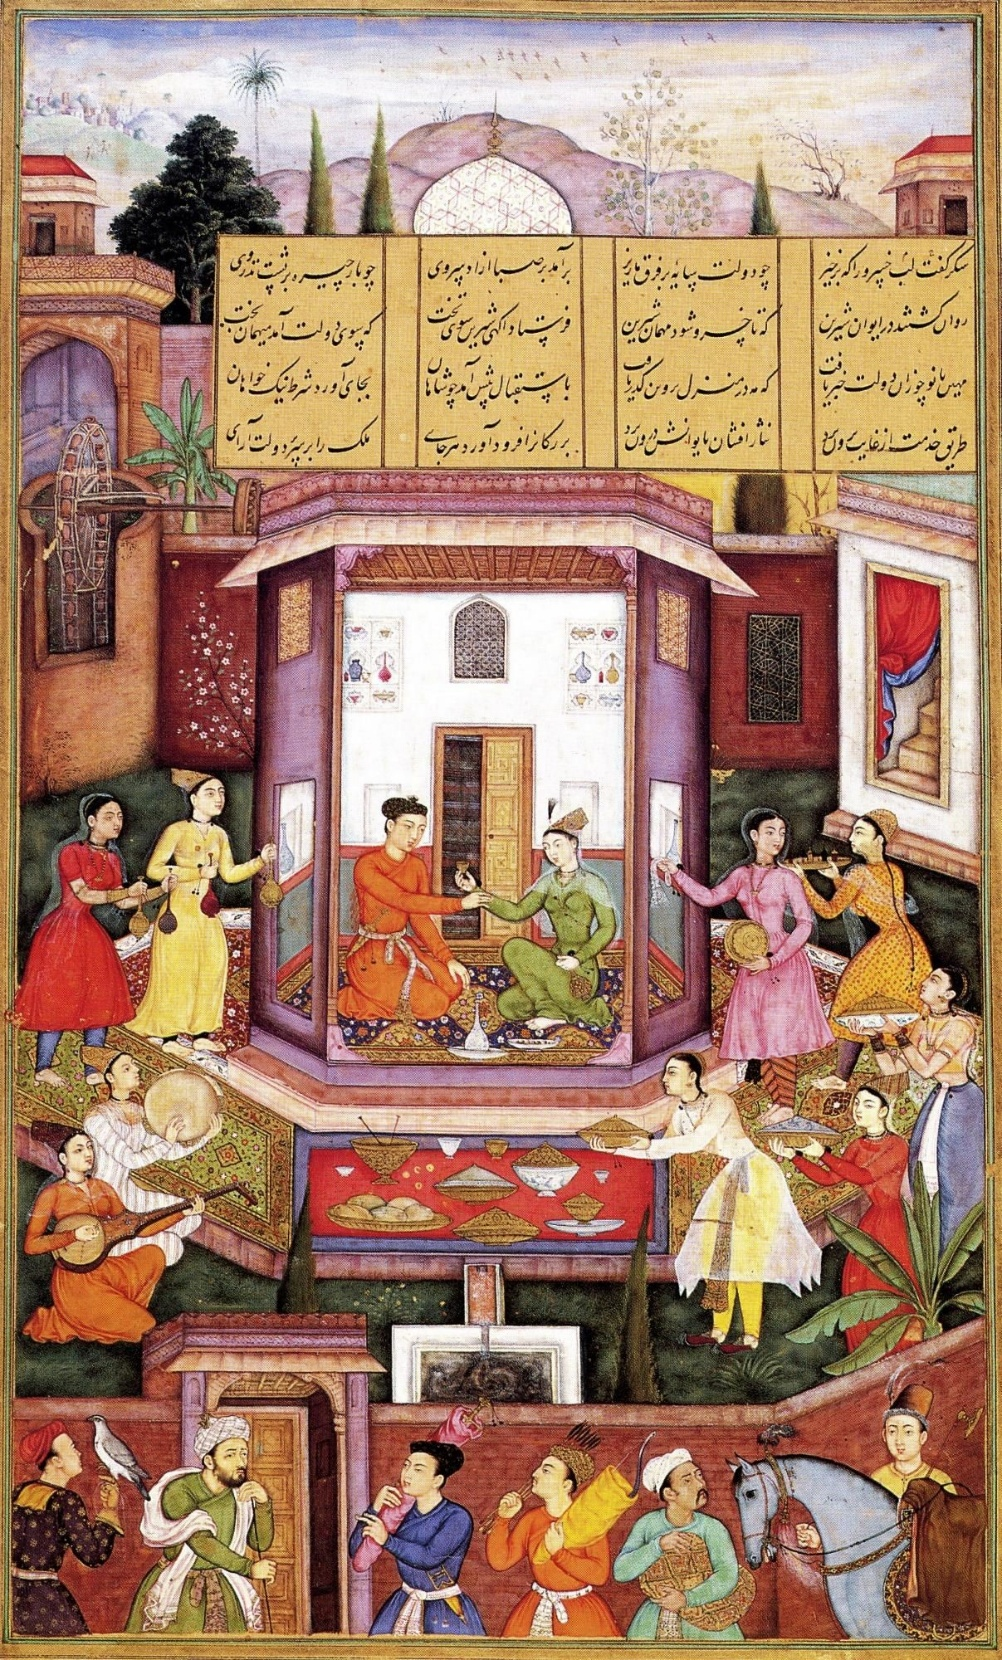
\includegraphics[width=0.85\linewidth]{image71.jpeg}
 \caption{Ilustração 6 do capítulo.}
 \label{fig:cap13-img6}
\end{figure}

No itinerário sufista, a alma trilha um caminho de aperfeiçoamento moral e gnose que antecipa a vida eterna. A salvação, entendida como reconciliação da alma com Deus, não é deixada apenas para o Além, mas buscada no presente mediante a aquisição do conhecimento místico (ma‘rifah) e da união amorosa com o Verdadeiro patheos.com. A famosa máxima sufi “morre antes de morrer” reflete a ideia de que o adepto deve “morrer” para o ego e para os apegos mundanos enquanto ainda vive, de modo a renascer espiritualmente já unido à vontade divina. Esse processo envolve atravessar diversos estados (a\d{h}wāl) e estações espirituais (maqāmāt): começa pelo arrependimento sincero (tawbah) e a renúncia das paixões, passa pela paciência, confiança absoluta em Deus (tawakkul), amor divino (mahabbah) e culmina na gnose (ma‘rifah) e no estado de aniquilação mística (fanā’) em Deus, seguido da subsistência (baqā’) pelo próprio Deus. No ápice, o sufi experimenta a união extática com o Divino, na qual o “eu” separado se dissolve como uma gota no oceano do Ser de Deus. Muitos poetas e santos sufis aludiram a essa união: Jalāl ad-Dīn Rumi, por exemplo, resumiu a trajetória da alma dizendo “Eu era imaturo; amadureci; e fui consumido”patheos.com -- versos que simbolizam a alma crua que, pelo fogo do amor divino, se cozinha e finalmente se queima em consumação na Luz de Deus. Nesse sentido, a “morte” para o sufi verdadeiro é vista não como fim trágico, mas como “noite de núpcias” da alma com o Amado eterno; Rumi chegou a celebrar o dia de sua morte como Shab-i Arūs, a “noite do casamento” com Deus.

A perspectiva sufi do pós-vida, portanto, enfatiza a continuidade entre a jornada terrena e a realidade eterna. Para os místicos, o Dia do Juízo não é apenas um evento futuro externo, mas corresponde à revelação (kashf) definitiva da Verdade que sempre esteve presente, embora velada aos olhos dos distraídos patheos.com. Eles ensinam que, na morte, “os véus serão retirados” e cada alma perceberá que tudo o que amou ou buscou não era senão reflexo do Único -- verdade esta já intuída pelo conhecedor durante a vida patheos.com. Como disse Ibn ‘Arabī: muitos pensam amar coisas particulares, mas ao morrer descobrirão que só Deus era o amado real, oculto atrás das aparências do mundo patheos.com. Consequentemente, o sufi se prepara para a morte buscando “ver através dos véus” já nesta vida, cultivando a visão do Real em todas as coisas. A salvação, então, deixa de ser um merecimento jurídico a ser decidido apenas no futuro, e torna-se sobretudo uma transformação ontológica da alma -- a qual desperta da ignorância para a consciência vívida de Deus, seja em vida, seja somente no momento pós-morte patheos.com. Essa concepção adota uma linguagem de luzes e revelações em vez de tribunais e sentenças: o Juízo Final, para os sufis, equivale à plena iluminação da alma pela Verdade divina, na qual toda ilusão se dissipa. De fato, muitos sufis aceitam os cenários de Paraíso e Inferno descritos nas escrituras, mas “os ressignificam como metáforas do desenvolvimento psíquico interior” e estados de consciência en.wikipedia.org. O Paraíso é, em última instância, o estado de plenitude na Realidade de Deus, enquanto o Inferno é a privação dessa Realidade, acompanhada do ardor do arrependimento e da vergonha espiritual.

Vale notar que essa ênfase no amor e na união mística levou alguns sufis a expressões teológicas ousadas. A lendária mística Rābi‘a al-‘Adawiyya (séc. VIII), por exemplo, orava: “Ó Deus, se Te adoro por medo do inferno, queima-me no inferno; se Te adoro pelo Paraíso, exclui-me do Paraíso; mas se Te adoro por Ti mesmo, não escondas de mim a Tua Beleza.” Com isso, Rābi‘a rejeitava qualquer motivação interesseira -- medo ou recompensa -- colocando o amor puro a Deus acima das imagens convencionais do além. Esse sentimento influenciou profundamente a mística islâmica posterior, de modo que o Amor Divino (ishq) passou a ser visto como a chave da bem-aventurança eterna, mais importante do que as delícias sensoriais frequentemente associadas ao Paraíso.

Conexões e Diálogos com o Cristianismo Medieval

As concepções islâmicas sobre o pós-vida -- tanto em sua forma normativa quanto em sua forma mística -- não permaneceram isoladas, mas dialogaram de várias maneiras com o imaginário e o pensamento cristão medieval. Entre os séculos XII e XIV, intensificaram-se os contatos culturais entre o mundo islâmico e a Europa latina, seja através da Península Ibérica e Sicília (onde muçulmanos, judeus e cristãos conviveram e trocaram saberes), seja via cruzadas, rotas comerciais e traduções de obras árabes para o latim. Esse intercâmbio permitiu que ideias escatológicas islâmicas deixassem ecos em determinadas obras, visões e teorias cristãs. A seguir, examinamos três âmbitos principais desse diálogo: (1) a literatura visionária medieval, (2) o misticismo cristão, e (3) a teologia escolástica e cosmologia.

Literatura Visionária: do Mi‘raj Islâmico às Visões Medievais Cristãs

Uma das áreas de convergência mais evidentes está nas narrativas visionárias de viagens ao além, muito populares em ambas as culturas. No Islã, a matriz desse gênero é a Ascensão (Mi‘rāj) do Profeta Muhammad, relatada tradicionalmente como uma experiência noturna em que Muhammad, guiado pelo anjo Gabriel, foi transportado milagrosamente de Meca a Jerusalém (no episódio do Isrā’) e, de lá, elevado através dos sete céus até a presença de Deus, vislumbrando também os horrores dos sete infernos ao longo do trajeto en.wikipedia.org. Nessa jornada, conhecida como Laylat al-Mi‘rāj, o Profeta encontra em cada céu os profetas precedentes (Adão, Jesus, João Batista, José, Idris, Moisés, Abraão), contempla as delícias reservadas aos bem-aventurados e os tormentos que aguardam os pecadores, e enfim alcança o Trono divino, onde recebe revelações e o dom da intercessão pela comunidade no Dia do Juízo en.wikipedia.org. Trata-se de uma visão de ultramundo ricamente detalhada nos hadiths e comentários posteriores, que fixou no imaginário islâmico a ideia de um cosmos estruturado em camadas de céus acima e regiões infernais abaixo, povoado de anjos, demônios e almas em trânsito.

Já no Ocidente cristão medieval, havia desde a Antiguidade Tardia relatos apócrifos de visitas ao além (por exemplo, a Visão de São Paulo ou Apocalipse de Pedro). Mas foi sobretudo a partir do século XII que floresceu um gênero de visões de além-túmulo em latim e nas línguas vernáculas, combinando moralidade cristã com elementos fantásticos. Um exemplo célebre é a Visão de Túndalo (Visio Tnugdali, composta em 1149), que narra a experiência de um cavaleiro irlandês, Túndalo, cuja alma, enquanto ele jaz em transe por três dias, é guiada por um anjo através dos reinos do Inferno e do Céu en.wikipedia.org. Durante o périplo, Túndalo testemunha horrendas punições infernais correspondentes a diversos pecados (num percurso que alude aos sete pecados capitais), bem como vislumbres das moradas celestiais dos justos ddd.uab.cat. Ao final, o anjo restitui a alma ao corpo e Túndalo desperta transformado, convertendo-se a uma vida de penitência en.wikipedia.org. Essa e outras visões medievais -- como a Visão de Alberico, a Visão do Monge de Eynsham e o relato do Purgatório de São Patrício -- delinearam uma “geografia” do além com notável riqueza de detalhes topográficos e morais en.wikipedia.org. O auge desse gênero, no fim da Idade Média, é sem dúvida a Divina Comédia de Dante Alighieri (início do séc. XIV), na qual o poeta, guiado pelo espírito de Virgílio e depois por Beatriz, percorre os círculos concêntricos do Inferno, escala a montanha do Purgatório e ascende através das esferas celestes até a visão de Deus.

Os paralelos entre essas viagens cristãs e o Mi‘rāj islâmico são inevitáveis. Estruturalmente, ambas envolvem um guia celestial conduzindo a alma do visionário por um itinerário ascendente/descendente através de múltiplos níveis de recompensa ou punição, com um encontro culminante (no caso de Dante e Muhammad) com o Divino no empíreo. A noção islâmica de sete céus sobrepostos e sete infernos inferiores en.wikipedia.org ecoa na divisão dantesca dos nove céus (sete esferas planetárias + firmamento das estrelas fixas + Primum Mobile) e dos nove círculos infernais, ainda que Dante os adapte a um esquema aristotélico-cristão. Vale ressaltar que o Islã possuía inclusive relatos de um local intermediário para espíritos imperfeitos, uma ideia semelhante ao Purgatório: o Alcorão menciona um al-A‘rāf, “muralha” ou limbo entre paraíso e inferno (Qur. 7:46), embora esse conceito não tenha se desenvolvido no dogma islâmico como o Purgatório no catolicismo. Ainda assim, a existência dessa “zona intermediária” na escatologia muçulmana pode ter sido conhecida pelos latinos e contrastada com suas próprias concepções emergentes de purgação temporal das almas.

Historicamente, há indicações de que textos islâmicos de escatologia visionária foram traduzidos e circulados na Europa medieval, podendo influenciar diretamente a literatura cristã. Em Castela, sob o reinado de Alfonso X (séc. XIII), foi traduzido do árabe para o castelhano e latim o chamado “Livro da Escada de Maomé” (Liber Scalae Machometi) en.wikipedia.org. Essa obra, derivada de compilações do Mi‘rāj, descreve em primeira pessoa a ascensão de Muhammad pelos sete céus e sete infernos, e é explicitamente mencionada em fontes posteriores como conhecida por Dante Alighieri en.wikipedia.org. De fato, já no início do século XX, o arabista Miguel Asín Palacios lançou a tese de que Dante teria se inspirado em grande medida em motivos da escatologia muçulmana na composição da Divina Comédia. Asín Palacios comparou detalhadamente a Comédia com narrativas do Mi‘rāj e outras lendas islâmicas, encontrando múltiplas correspondências temáticas: a figura de um profeta ou santo viajando no além, as etapas ascendentes do universo, encontros com almas e anjos de diferentes categorias, a presença de um paraíso sensual com jardins e rios, etc. en.wikipedia.org. Ele argumentou que Dante possivelmente teve acesso, através de traduções latinas ou da convivência com intelectuais em Florença e Bolonha, a relatos islâmicos (como o Liber Scalae), adaptando-os genialmente ao contexto cristão. Essa hipótese gerou intenso debate acadêmico. Alguns estudiosos ocidentais reconheceram a possibilidade de influência islâmica em Dante, especialmente considerando os contatos culturais da época e o fato de que Brunetto Latini -- mentor de Dante -- esteve na Espanha em meados do séc. XIII, possivelmente tomando conhecimento de materiais árabes bibliotecanatalie.com. Outros, contudo, ponderam que Dante também podia beber de uma tradição visionária cristã já existente (por exemplo, a Visão do Túndalo fora amplamente difundida e traduzida em vários idiomas europeus commons.wikimedia.org) e de fontes clássicas e bíblicas, sem necessidade de um “empréstimo” direto do Islã. Seja como for, a própria discussão é indicativa de diálogo intelectual medieval: contemporâneos de Dante sabiam da existência da “Lenda da Ascensão de Maomé”, e alguns polemistas cristãos até acusavam Muhammad de plagiar apócrifos cristãos (como o Apocalipse de Paulo) para compor sua narrativa da Noite da Ascensão. Em suma, as semelhanças estruturais entre o Mi‘rāj e as visões cristãs -- culminando com a obra dantesca -- sugerem ao menos um imaginário escatológico compartilhado, onde ideias viajavam de um contexto a outro. A Visão de Túndalo, por exemplo, foi escrita originalmente em latim por um monge irlandês na Alemanha, mas rapidamente se espalhou e ganhou versões em diversas línguas (inclusive no medievo ibérico). Essa circulação torna difícil traçar influências unilaterais, mas permite afirmar que havia um clima intelectual comum explorando os mistérios do além, no qual muçulmanos e cristãos mutuamente conheciam e comentavam suas narrativas visionárias.

Misticismo Cristão e Parâmetros Sufis

No campo do misticismo, também se identificam paralelos e possíveis influências entre sufismo islâmico e espiritualidade cristã medieval. Na Espanha muçulmana (al-Andalus) e posteriormente na Espanha cristã recém-reconquistada, houve casos notáveis de confluência mística. Miguel Asín Palacios, em sua obra El Islam cristianizado (1931), investigou a influência de ideias de Ibn ‘Arabī e outros sufis sobre místicos espanhóis posteriores en.wikipedia.org. De fato, filósofos e místicos muçulmanos de al-Andalus, como Ibn Masarra, Ibn ‘Arabī de Múrcia e outros, desenvolveram teorias da Unidade do Ser (wahdat al-wujūd) e do amor divino que guardam semelhança com noções de místicos cristãos como Mestre Eckhart na Alemanha ou, mais tarde, São João da Cruz e Santa Teresa d’Ávila na Espanha do Renascimento. Embora uma influência direta seja difícil de provar em todos os casos, a presença de literatura sufi em tradução é atestada em alguns círculos cristãos. Por exemplo, textos de mística islâmica teriam sido traduzidos para o castelhano a pedido do rei Afonso X e circulado entre estudiosos. Além disso, através dos escritos de João Damasceno e outros polemistas orientais, alguma informação sobre ascetas muçulmanos (como os “ensimesmados” sufis) chegou à Europa.

Conceitos específicos apresentam ressonâncias intrigantes. A metáfora do caminho interior e da ascensão da alma é comum a sufis e místicos cristãos. Assim como os sufis falam em maqāmāt e fanā’, místicos cristãos medievais (sob influência da teologia neoplatônica do Pseudo-Dionísio) descrevem vias ou degraus da perfeição espiritual -- via purgativa, iluminativa e unitiva -- pelas quais a alma abandona o apego ao mundo sensível e se une a Deus numa espécie de casamento místico. A linguagem de amor esponsal usada por místicos como São Bernardo de Claraval e, mais tarde, Teresa d’Ávila, encontra paralelo na poesia sufista, repleta de imagens de amante e Amado. Por exemplo, a noção de “feridas de amor” da alma que arde de desejo por Deus aparece tanto nos sermões de Bernardo (inspirado no Cântico dos Cânticos) quanto nos versos de poetas sufis como Hafiz ou Ibn al-Fāri\d{d}. A própria figura da noite escura da alma, celebrizada por São João da Cruz, lembra o “estado de ausência” descrito por sufis -- uma travessia de desolação necessária antes da iluminação final.


\begin{figure}[ht]
 \centering
 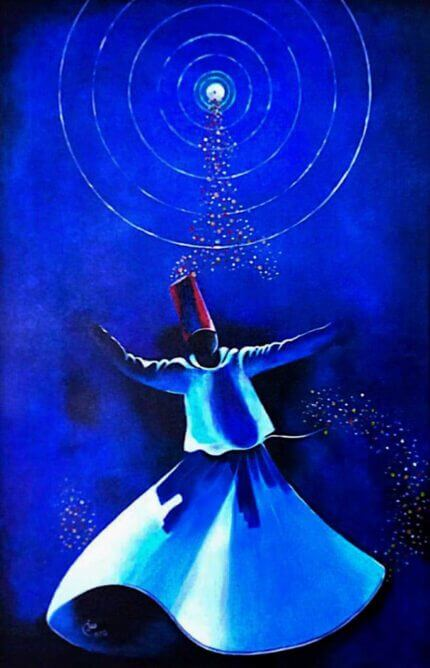
\includegraphics[width=0.85\linewidth]{image72.jpeg}
 \caption{Ilustração 7 do capítulo.}
 \label{fig:cap13-img7}
\end{figure}

Arte contemporânea representando um dervixe rodopiante em estado de êxtase místico. A imagem captura a essência da espiritualidade sufi, onde a "morte antes de morrer" ao ego permite ao adepto experimentar a união com o Divino ainda em vida, antecipando a verdadeira salvação que consiste na reconciliação da alma com Deus.

Há casos documentados de interação direta: no séc. XIII, em Maiorca, o beato Raimundo Lúlio (Ramon Llull), um dos primeiros missionários e pensadores a estudar árabe, travou contato com obras islâmicas. Embora Lúlio combatesse o Islã teologicamente, adotou em seus escritos místicos certa terminologia de amor cortês e talvez ecos sufi. Já no séc. XVI, quando a Espanha absorveu as influências de séculos de cultura islâmica, alguns estudiosos modernos veem analogias entre, por exemplo, a “Noite Escura” de João da Cruz e o conceito sufi de fanā’ (aniquilação no Amado). A precaução aqui é necessária: essas semelhanças podem derivar de convergência espontânea em tradições espirituais diferentes, sem contato histórico direto. Contudo, a escola espanhola de espiritualidade possuía uma familiaridade indireta com o legado sufista, pois durante a Reconquista muitos tratados árabes caíram em mãos cristãs, e alguns convertidos do Islã ao cristianismo (moriscos) atuaram como transmissores culturais.

Além disso, figuras universais como Plotino e a filosofia neoplatônica influenciaram tanto sufis quanto místicos cristãos, criando um vocabulário comum de êxtase, ascensão intelectual e união com o Uno. Assim, mesmo sem empréstimo consciente, um místico cristão podia desenvolver ideias próximas às sufis porque ambos beberam de fontes neoplatônicas semelhantes (como a ideia da reemergência da centelha divina à sua origem). Exemplificando, o conceito de deificação (theosis) na mística cristã ortodoxa -- tornar-se um “com-participante da natureza divina” -- ecoa a noção sufi de “insān kāmil” (homem perfeito) que reflete plenamente os atributos divinos, e ambos remetem à noção platônica de retorno da alma ao Bem supremo.

Importante notar que, na Idade Média, também houve reações negativas no campo místico: setores mais rígidos da Igreja viam com suspeita ideias de “união essencial” que lembrassem panteísmo -- assim como juristas muçulmanos criticavam sufis como al-Hallāj, que proclamou “Ana al-Haqq” (“Eu sou a Verdade [Divina]”). Apesar disso, o legado sufista de amor e mergulho no divino acabou por enriquecer a piedade cristã através, por exemplo, da poesia de São João da Cruz, que muitos compararam à dos sufis persas pela profundidade e beleza.

Teologia Escolástica e Intercâmbio Filosófico-Cosmológico

No domínio da teologia e filosofia, a escolástica medieval engajou-se intensamente com as ideias provenientes do mundo islâmico, especialmente a partir do século XII, quando houve a grande tradução de textos árabes para o latim. Dentre esses textos estavam não apenas obras de Aristóteles e outros gregos preservados pelos muçulmanos, mas também tratados originais de filósofos islâmicos como Avicena (Ibn Sina), Averróis (Ibn Rushd), Al-Farabi, além de compêndios enciclopédicos sobre cosmologia e ciências naturais. Esses escritos trouxeram novas concepções sobre o cosmos, a alma e a vida após a morte que desafiaram e enriqueceram o pensamento cristão.

Um impacto fundamental foi a adoção do modelo cosmológico aristotélico-ptolemaico, mediado pelos comentaristas árabes. Obras como o Almagesto de Ptolemeu e o Tratado dos Céus de Aristóteles, comentadas por Averróis e Avicena, delineavam um universo de esferas concêntricas em número definido (geralmente nove esferas celestes). Os escolásticos latinos -- Alberto Magno, Tomás de Aquino e outros -- absorveram essa cosmologia esférica, integrando-a à teologia cristã do além. Dante exemplifica isso de forma literária: sua descrição dos céus do Paraíso (Lua, Mercúrio, Vênus, Sol, Marte, Júpiter, Saturno, Estrelas Fixas, Primum Mobile e Empíreo) combina a astronomia recebida dos árabes com a hierarquia angélica e os estados de beatitude. Ora, a ideia de várias camadas celestiais habitadas por seres luminares e almas aventurosas também era familiar aos muçulmanos (os sete céus do Mi‘rāj, ocupados por profetas). Ao incorporar a cosmologia esférica “arábico-aristotélica”, os cristãos medievalmente aproximaram-se estruturalmente da visão islâmica de um cosmos graduado -- embora, naturalmente, divergindo em conteúdo teológico (por exemplo, Dante coloca santos cristãos onde o Islã coloca profetas ou anjos).

Mais diretamente no campo escatológico, os escolásticos confrontaram as teorias islâmicas sobre a alma e a ressurreição. Avicena particularmente influenciou esse debate: ele sustentava, com base filosófica, a imortalidade da alma individual, mas via o estado pós-morte principalmente como espiritual (a alma experimentando felicidade ou sofrimento intelectualmente, não através de sentidos corpóreos). Avicena reconhecia a ressurreição corporal por fé religiosa, mas sua filosofia tendia a minimizar a necessidade do corpo no gozo ou pena da alma imortal. Quando Tomás de Aquino e outros leram as obras de Avicena (em latim, Liber de Anima e Metafísica, entre outras), viram nisso um potencial conflito com a doutrina cristã, que exige a ressurreição da carne para a plenitude do prêmio ou castigo. Aquino chega a criticar explicitamente “o Comentador” (Averróis) e “o Filósofo árabe” (Avicena) em pontos sobre a natureza da alma. Por exemplo, Averróis propunha que apenas o Intelecto universal é eterno, enquanto as individualidades se perdem -- ideia inadmissível para a fé cristã na vida eterna pessoal. Assim, os pensadores cristãos reagiram refinando suas próprias formulações: Aquino reafirmou que a alma separada, embora já receba um juízo particular após a morte, anseia pela reunião com o corpo glorioso na ressurreição, pois o ser humano completo é corpo e almareddit.com. Em refutações aos árabes, escolásticos enfatizaram que o sofrimento ou deleite plenos requerem a dimensão corpórea restaurada, tornando necessária a ressurreição final -- contra qualquer visão puramente intelectualizada do pós-vida.

Ao mesmo tempo, ideias e metáforas islâmicas foram adaptadas em contextos cristãos. Por exemplo, a imagem da ponte fina sobre o Inferno (as-\d{s}irā\d{t}) existente na escatologia muçulmana aparece em versões de visões cristãs medievais, às vezes como uma ponte ou tronco estreito que as almas devem cruzar -- possivelmente derivada de tradições escatológicas orientais (zoroastrianas e islâmicas)hell-on-line.org. Igualmente, a noção do Livro das Obras e da pesagem das almas, embora já presente no Cristianismo (e no Egito antigo), ganhou detalhes nas descrições islâmicas que podiam circular e enriquecer o imaginário popular cristão via contato cultural.

A circulação de tratados cosmológicos e filosóficos em tradução também expôs teólogos latinos a conceitos cosmográficos islâmicos. Por exemplo, o tratado Liber de ascensione (Kitāb al-Mi‘rāj), além de sua função moral-religiosa, trazia descrições da estrutura do universo (estrelas, planetas, anjos regentes de cada esfera, etc.) que ampliaram a cosmologia cristã. Tradutores como Gerardo de Cremona e Hermann de Carinthia verteram para o latim obras árabes que mapeavam o cosmo de acordo com as concepções de astrônomos muçulmanos (p. ex., o Kitāb al-‘Ālam e o Hay’at al-‘alam). Tais conhecimentos permitiram que autores cristãos concebesses o cenário do além de forma mais ordenada e “científica”. Dante novamente ilustra isso: ele conhecia provavelmente o Liber de Mundo (tradução latina de um texto árabo-arábico pseudo-aristotélico) e faz referências que sugerem familiaridade com a tradição científica islâmica (por exemplo, a divisão do globo entre hemisfério habitado e hemisfério aquoso, conceitos advindos via árabes).

Por fim, como reagiram os teólogos cristãos às visões islâmicas de Paraíso e Inferno em termos apologéticos? Em controvérsias inter-religiosas, escritores latinos frequentemente criticavam o Islã por pintar um Paraíso materialista e voluptuoso -- com banquetas, rios de mel e virgens --, contrapondo-o à visão mais “espiritual” e contemplativa do Céu cristão. Essa crítica aparece já em autores como Pedro, o Venerável (séc. XII) e depois em Ricoldo da Montecroce (séc. XIII). Porém, curiosamente, dentro da escolástica, alguns argumentaram que a justiça divina deveria conceder alguma forma de prazer sensível aos bem-aventurados cristãos também, já que eles ressuscitarão em carne. Assim, pode-se dizer que o quadro islâmico acabou forçando esclarecimentos: teólogos latinos afirmaram que, sim, no Céu cristão haverá gozo do corpo glorificado, mas sem pecado ou concupiscência -- diferenciando-o do estereótipo que faziam do jannah islâmico. Por outro lado, místicos cristãos, influenciados pelo ideal sufi do amor desinteressado, enfatizaram cada vez mais que o supremo deleite do Paraíso é a Visão Beatífica de Deus, um conceito análogo ao “ver o Rosto de Deus” na teologia islâmica (o Alcorão 75:22-23 menciona que os rostos dos fiéis resplandecerão ao olhar para seu Senhor). Assim, até mesmo naquilo que os cristãos criticavam no Islã, havia terreno para reflexão e eventual assimilação depurada.

Em suma, o diálogo medieval islâmico-cristão no tocante à escatologia foi ricamente multifacetado. Seja através de textos visionários compartilhados ou paralelos, seja pelo ecumenismo dos místicos em busca da verdade última, seja pelo debate filosófico-teológico nas universidades, o pós-vida imaginado por muçulmanos e cristãos interagiu de modo a moldar ambas as civilizações. Essa interação deixou traços na literatura (como as comparações entre o Mi‘rāj e a Divina Comédia), na mística (como as afinidades entre sufis e contemplativos cristãos) e na teologia (como as respostas escolásticas a Avicena e outros). Acadêmicos modernos, como Asín Palacios, dedicaram-se a desvendar essas conexões, mostrando, por exemplo, que Dante pode ter se inspirado em motivos muçulmanos en.wikipedia.org, ou que a mística espanhola deve algo à herança sufista de al-Andalus en.wikipedia.org. Embora nem todas as teses sejam consensuais, está claro que as ideias escatológicas viajaram entre as culturas. O fascínio universal por questões do além-túmulo permitiu que muçulmanos e cristãos medievalmente compartilhassem visões e perguntas -- sobre céu e inferno, anjos e demônios, destino da alma e justiça divina --, deixando um legado de influência mútua que enriqueceu o pensamento religioso de ambos os mundos.


\begin{figure}[ht]
 \centering
 \includegraphics[width=0.85\linewidth]{image73.jpeg}
 \caption{8. Liber Scalae Machometi - O Livro da Escada de Maomé}
 \label{fig:cap13-img8}
\end{figure}


\begin{figure}[ht]
 \centering
 \includegraphics[width=0.85\linewidth]{image74.jpeg}
 \caption{8. Liber Scalae Machometi - O Livro da Escada de Maomé}
 \label{fig:cap13-img9}
\end{figure}

Ilustração do "Conto de Bayad e Riyad" (final século XIII), único manuscrito ilustrado conhecido que sobreviveu dos mais de 8 séculos de presença muçulmana na Espanha. Representa o ambiente cultural de Al-Andalus onde se desenvolveram intercâmbios intelectuais entre tradições islâmicas e cristãs, incluindo conceitos escatológicos e narrativas visionárias.

8. Liber Scalae Machometi - O Livro da Escada de Maomé


\begin{figure}[ht]
 \centering
 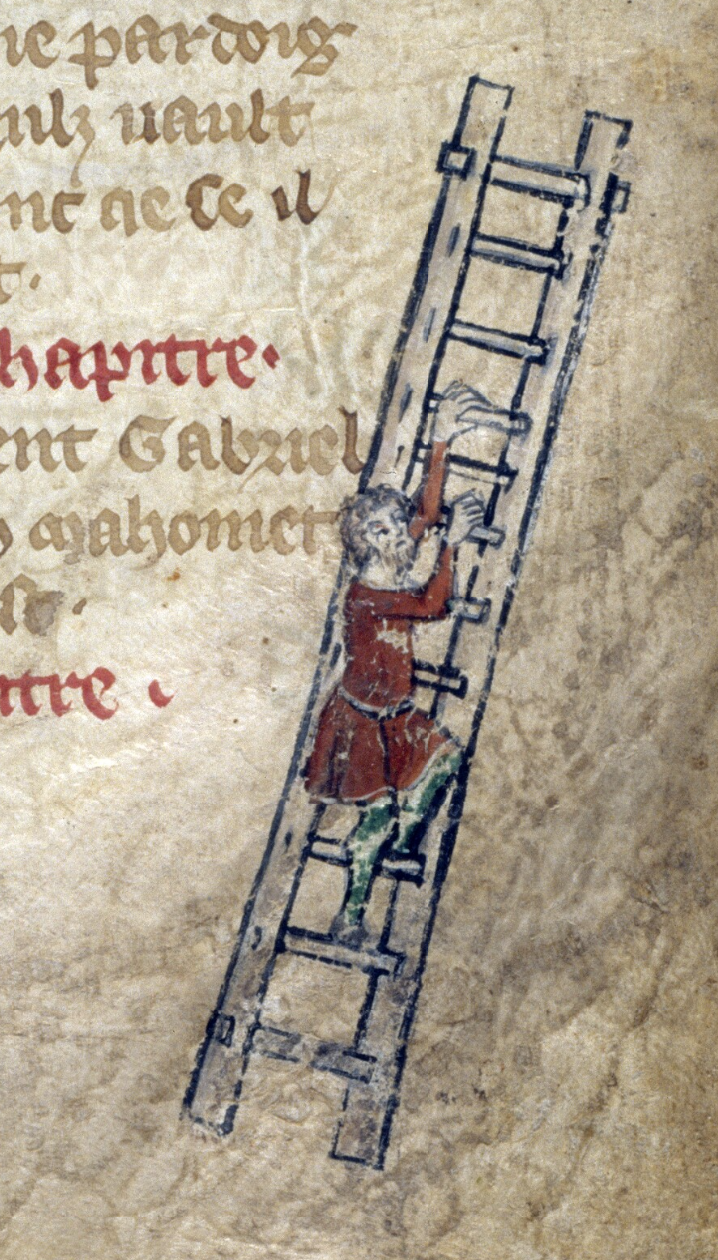
\includegraphics[width=0.85\linewidth]{image75.png}
 \caption{9. Cosmologia dos Sete Céus}
 \label{fig:cap13-img10}
\end{figure}


\begin{figure}[ht]
 \centering
 \includegraphics[width=0.85\linewidth]{image76.png}
 \caption{9. Cosmologia dos Sete Céus}
 \label{fig:cap13-img11}
\end{figure}

9. Cosmologia dos Sete Céus


\begin{figure}[ht]
 \centering
 \includegraphics[width=0.85\linewidth]{image77.jpeg}
 \caption{Ilustração 12 do capítulo.}
 \label{fig:cap13-img12}
\end{figure}


\begin{figure}[ht]
 \centering
 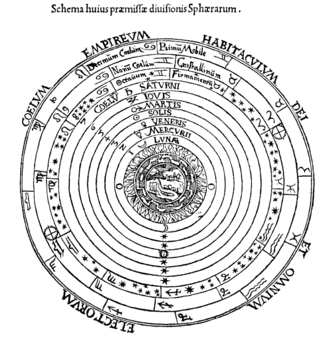
\includegraphics[width=0.85\linewidth]{image78.png}
 \caption{Ilustração 13 do capítulo.}
 \label{fig:cap13-img13}
\end{figure}

Diagrama do sistema ptolemaico de esferas celestiais concêntricas, modelo cosmológico adotado tanto por astrônomos muçulmanos quanto por pensadores cristãos medievais. Esta estrutura de nove esferas (sete planetárias + estrelas fixas + Primum Mobile) forneceu o framework para as viagens visionárias em ambas as tradições, desde o Mi'raj até a jornada de Dante através do Paraíso.


\begin{figure}[ht]
 \centering
 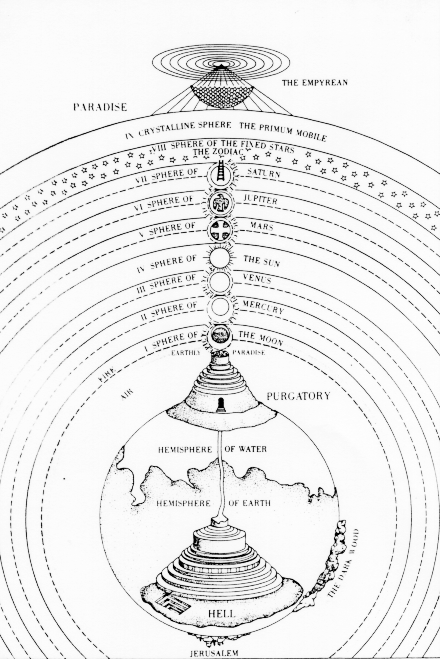
\includegraphics[width=0.85\linewidth]{image79.png}
 \caption{Ilustração 14 do capítulo.}
 \label{fig:cap13-img14}
\end{figure}

Representação esquemática da cosmologia de Dante na Divina Comédia, mostrando os nove círculos do Inferno (embaixo), a montanha do Purgatório (centro) e as esferas celestiais do Paraíso (acima). Esta estrutura reflete a síntese dantesca entre a cosmologia aristotélica mediada pelos comentaristas árabes e a teologia cristã, possivelmente influenciada por elementos do Mi'raj islâmi

Fontes selecionadas: As bases normativas islâmicas foram sintetizadas de fontes primárias e sumários teológicos en.wikipedia.org. As concepções místicas sufis apoiam-se em escritos de Rumi, Ibn ‘Arabī e estudos modernos sobre sufismo patheos.com en.wikipedia.org. Para as comparações históricas, utilizamos estudos acadêmicos sobre a Liber Scalae Machometi e Dante en.wikipedia.org, bem como análises da visão de Túndalo e literatura visionária en.wikipedia.org. A influência intelectual árabe na cristandade foi discutida com base em historiografia do intercâmbio filosófico medieval en.wikipedia.org. Estas referências evidenciam a complexidade e a profundidade do tema, demonstrando como as visões do pós-vida no Islã dialogaram criativamente com o imaginário cristão medieval.


% --- Capítulo 14: A Síntese Dantesca: Culminação Medieval da Imaginação Infernal e Diálogo Intercultural ---
\chapter[A Síntese Dantesca]{A Síntese Dantesca: Culminação Medieval da Imaginação Infernal e Diálogo Intercultural}
\epigraph{A Divina Comédia de Dante representa o apogeu medieval da imaginação infernal --- integrando tradições clássicas, cristãs e islâmicas numa visão abrangente de punição eterna, com paralelos profundos com o Mi‘rāj que revelam um framework escatológico comum enraizado no monoteísmo abraâmico.}

O período medieval representa momento culminante na elaboração artística e teológica de conceitos infernais, atingindo seu apogeu na Divina Comédia de Dante Alighieri (c. 1308-1320). Esta síntese extraordinária integra tradições clássicas, cristãs, e islâmicas numa visão compreensiva de punição eterna que estabelece paradigmas representacionais duradouros. A obra dantesca emerge de contexto intelectual rico, onde literatura visionária, sistematização escolástica, iconografia gótica, e intercâmbio cultural entre civilizações criaram ambiente propício para síntese multicultural sem precedentes.

Pesquisas acadêmicas recentes identificaram conexões profundas entre as tradições escatológicas abraâmicas, particularmente paralelos estruturais e temáticos entre o Mi'raj islâmico e narrativas visionárias cristãs. Estudos comparativos revelam que essas semelhanças não são meramente coincidentais, mas refletem framework escatológico comum enraizado na crença monoteísta num Deus transcendente criador do universo.


\begin{figure}[ht]
 \centering
 \includegraphics[width=0.85\linewidth]{image80.jpeg}
 \caption{2. Precedentes na Literatura Visionária Medieval}
 \label{fig:cap14-img1}
\end{figure}

Célebre fresco de Domenico di Michelino (1465) na Catedral de Florença mostrando Dante Alighieri diante de sua visão do além. À esquerda veem-se os círculos do Inferno, ao centro a montanha do Purgatório, e à direita as esferas celestiais do Paraíso - estrutura cosmológica que ecoa elementos do Mi'raj islâmico.

2. Precedentes na Literatura Visionária Medieval

A literatura visionária medieval desenvolve geografia sistemática de reinos pós-morte que antecipa e influencia a síntese dantesca. Textos fundamentais incluem:

A Visão de Dryhthelm (Beda, c. 731) introduz elementos cruciais como divisão topográfica tripartite entre vale de lamentações (futuro inferno), montanha purificativa (futuro purgatório), e prados celestiais (futuro paraíso). Esta geografia estabelece modelo estrutural que influencia toda literatura visionária posterior.


\begin{figure}[ht]
 \centering
 \includegraphics[width=0.85\linewidth]{image81.jpeg}
 \caption{Ilustração 2 do capítulo.}
 \label{fig:cap14-img2}
\end{figure}

Iluminura de Simon Marmion (século XV) retratando Túndalo sofrendo o transe que precede sua viagem visionária ao além, conforme narrado na "Visão de Túndalo" (Visio Tnugdali, 1149). Esta obra cristã apresenta paralelos estruturais notáveis com o Mi'raj islâmico.

A Visão de Túndalo (Visio Tnugdali, c. 1149) oferece descrições detalhadas de monstros infernais e punições corporais que influenciam iconografia posterior. O texto irlandês descreve criaturas como Acheron (demônio de mil olhos) e Fergus (gigante torturador), estabelecendo precedentes para representações que Dante refinará. A ponte estreita sobre abismos flamejantes ecoa tradições orientais e prefigura travessias perigosas no cosmos dantesco.

O Tractatus de Purgatorio Sancti Patricii (séc. XII) desenvolve conceito de purgação temporal através de sofrimentos graduados, introduzindo ideia de que diferentes intensidades de pecado requerem diferentes durações e tipos de punição. Esta sistematização temporal complementa a geográfica, criando framework escatológico fundamental para Dante.

Estas visões apresentam geografia estratificada onde diferentes pecados recebem punições específicas correspondentes, estabelecendo princípio de contrapasso que Dante elaborará sistematicamente. O conceito emerge gradualmente: punições refletem natureza essencial dos pecados, criando sistema ético onde justiça divina se manifesta através de correspondências precisas entre culpa moral e castigo físico.

A Sistematização Escolástica: Tomás de Aquino e a Teologia do Inferno

A síntese escolástica medieval, culminando na obra de Tomás de Aquino (1225-1274), ofereceu uma sistematização teológica robusta que serviu de arcabouço doutrinal para as representações artísticas do inferno. Em sua Summa Theologica, Aquino apresenta uma análise detalhada que estabelece a ortodoxia teológica sobre a escatologia e define os elementos essenciais da concepção do inferno na perspectiva cristã medieval. Para Aquino, o inferno não é uma metáfora, mas sim uma realidade ontologicamente necessária, derivada da perfeição da justiça divina. Nas Questões 69 e 70 do Suplemento da Summa Theologica, ele desenvolve uma teoria sistemática do inferno abordando múltiplas dimensões desse estado pós-morte.

Primeiramente, Aquino discute a localização e a natureza física do inferno. Ele situa o inferno no centro da Terra -- posição que simboliza o afastamento máximo em relação a Deus, já que, na cosmologia medieval, o centro do mundo material é o ponto mais distante da perfeição divina nos céus. O fogo infernal, segundo Aquino, é simultaneamente corpóreo e real, porém dotado de propriedades sobrenaturais. Isso significa que esse fogo pode afetar tanto os corpos ressuscitados quanto os espíritos, infligindo tormentos perpétuos sem jamais consumi-los completamente. Tal descrição visa conciliar a ideia de um sofrimento físico no além com a imortalidade da alma e do corpo glorificado (ou neste caso, condenado).

Aquino distingue, ademais, duas modalidades de punição no inferno: a poena sensus e a poena damni. A pena dos sentidos (poena sensus) corresponde aos tormentos sensíveis -- os sofrimentos físicos como o fogo, a sede, a escuridão e outras formas de aflição corporal descritas tradicionalmente. Já a pena do dano (poena damni) consiste na privação eterna da visão beatífica, isto é, na impossibilidade definitiva de contemplar Deus para sempre. De acordo com Aquino, essa privação do Sumo Bem é o aspecto mais grave da pena infernal, pois representa a frustração completa do fim último do ser humano (que, para a teologia cristã, é a comunhão com Deus). A conjunção dessas duas penas -- sentidos e dano -- produz um sofrimento total e absoluto, que abrange todas as dimensões da pessoa condenada, tanto corporal quanto espiritual.

Outro ponto central na teologia aquiniana do inferno é a sua eternidade e irreversibilidade. O caráter eterno da condenação infernal, segundo Aquino, deriva da condição da alma após a morte: uma vez separada do corpo, a alma fixa a sua vontade no estado em que se encontra no momento da morte. Assim, se alguém morre em pecado mortal (isto é, deliberadamente afastado de Deus), permanece para sempre nessa disposição obstinada, incapaz de arrepender-se ou de mudar sua orientação fundamental. Por essa razão, a justiça divina determina que a punição do inferno seja irremissível e perpétua -- não por uma limitação da misericórdia de Deus, mas porque a própria criatura se colocou, de forma definitiva, fora do alcance dessa misericórdia ao morrer em estado de rejeição a Ela. A eternidade do inferno reflete, pois, a escolha livre e permanente da criatura que recusou submeter-se à ordem do amor divino.

Por fim, Tomás de Aquino aborda a graduação das penas infernais. Para assegurar a justiça proporcional dos castigos, diferentes graus de tormento correspondem aos diferentes tipos e gravidades de pecados cometidos em vida. Aqueles que cometeram faltas mais leves sofreriam penas menos intensas do que os autores de pecados particularmente graves e perversos. Esse princípio de gradação punitiva garante que a justiça divina seja ao mesmo tempo equitativa e exemplar: cada condenado recebe uma pena condizente com sua culpa. Essa concepção de um inferno estruturado em níveis ou esferas de sofrimento gradativo forneceu a base intelectual para a imaginação artística e literária do inferno nos séculos seguintes -- em especial, serviu de inspiração para a notável arquitetura do inferno apresentada por Dante Alighieri no início do século XIV.

A síntese escolástica, que culmina na obra de Tomás de Aquino (1225-1274), oferece uma sistematização teológica rigorosa que fornece o arcabouço doutrinal para as representações artísticas do inferno. A Summa Theologica apresenta uma análise detalhada e metódica que estabelece a ortodoxia teológica sobre a escatologia cristã, influenciando profundamente a imaginação medieval.


\section*{A Síntese Dantesca: Arquitetura Infernal e Multiculturalismo Teológico}
\addcontentsline{toc}{section}{A Síntese Dantesca: Arquitetura Infernal e Multiculturalismo Teológico}

Na Divina Comédia, Dante concebe o inferno precisamente como uma série de círculos concêntricos dispostos em forma de um imenso cone invertido no interior da Terra -- configuração que, segundo o poeta, se formou quando Lúcifer foi expulso dos céus e caiu sobre o mundo. Essa topografia dantesca do inferno combina o arcabouço doutrinal escolástico com influências de diversas tradições culturais, resultando numa representação de grande complexidade simbólica e precisão quase matemática. A localização central do inferno retomada por Dante reflete diretamente a cosmologia aristotélica adotada por Aquino e pelos pensadores medievais: o centro do universo sublunar como lugar da materialidade pesada e corrupta. No entanto, Dante expande e detalha essa visão cosmológica de modo sem precedentes, transformando especulações filosóficas em uma paisagem infernal vívida. Elementos como o rio Aqueronte, os portões da cidade de Dite (capital do inferno dantesco) e o lago congelado Cocite no fundo do inferno compõem uma geografia moral intrincada. Cada acidente geográfico e cada círculo têm um significado alegórico preciso, funcionando simultaneamente como símbolo teológico-moral (da natureza e gravidade dos pecados ali punidos) e como cenário narrativo para os episódios do poema.

A estrutura concêntrica do inferno de Dante, com nove círculos em sucessão descendente, reflete claramente a ideia de gradação das penas conforme a gravidade do pecado -- ideia essa que, como vimos, estava presente na teologia escolástica de Aquino. Contudo, Dante não se limitou às fontes latinas e cristãs; ele também incorporou ao seu inferno elementos oriundos de outras culturas, num gesto que podemos chamar de um ecletismo multicultural medieval. Por exemplo, a concepção de múltiplos níveis infernais apresenta paralelos com a tradição islâmica, na qual se fala de sete infernos ou sete portões do inferno. Há indícios de que Dante, através de traduções latinas ou do contato indireto com a cultura árabe, conhecia relatos escatológicos muçulmanos. A inclusão do profeta Maomé no oitavo círculo do inferno (entre os semeadores de discórdia, dilacerados eternamente por demônios) é particularmente reveladora dessa confluência de influências. As vívidas descrições de punições específicas para diversos tipos de pecadores na Divina Comédia -- algumas das quais têm correspondência em textos islâmicos medievais sobre o pós-vida -- sugerem que Dante adaptou motivos extrabíblicos dentro de uma moldura cristã ortodoxa, enriquecendo sua obra com um imaginário global para transmitir verdades morais e teológicas.

Em suma, a sistematização escolástica oferecida por Tomás de Aquino forneceu os fundamentos conceituais sobre os quais se ergue a teologia do inferno na Idade Média: um inferno dotado de localidade, de realismo físico e metafísico, de penas múltiplas (sensíveis e espirituais), eternas e proporcionais ao delito. Essa base doutrinal permitiu a autores e artistas posteriores dar forma concreta a esse mundo de punições. Dante Alighieri, apoiando-se nesses fundamentos e dialogando com diversas fontes culturais, levou essa concepção ao auge ao criar uma verdadeira "síntese dantesca": uma monumental arquitetura infernal literária que alia a ortodoxia teológica a um rico multiculturalismo medieval, produzindo uma visão do inferno tão universal em seu significado quanto detalhada em sua imaginação.

A estrutura de círculos concêntricos e descendentes ecoa notavelmente os sete infernos (jahannam) da tradição escatológica islâmica, descritos no Alcorão e elaborados em textos como a Escada de Maomé (Kitab al-Miraj), que circulava na Europa medieval. A controversa presença de Maomé no oitavo círculo, entre os semeadores de discórdia, e a especificidade de certas punições --- como a contrapasso que faz os corpos dos condenados refletirem seus pecados --- sugerem familiaridade de Dante com narrativas escatológicas muçulmanas, possivelmente mediadas por traduções latinas ou contatos culturais na Sicília e Espanha.

Dante desenvolve o princípio do contrapasso (do latim contra + patior, "sofrer o contrário") muito além das tradições precedentes, elevando-o a um sistema sofisticado de justiça poética que transcende a mera retaliação. Este conceito, embora tenha raízes na lei do talião bíblica ("olho por olho") e em tradições escatológicas islâmicas e apócrifas cristãs, alcança em Dante uma complexidade filosófica e simbólica sem precedentes. Cada punição não apenas castiga o pecado, mas o revela, tornando visível exteriormente a deformação moral interior que o pecador escolheu em vida.

O poeta florentino articula o contrapasso através de duas modalidades principais, cada uma revelando diferentes aspectos da justiça divina:

1. Contrapasso por Analogia (Similitude)

Nesta modalidade, a punição espelha ou imita o pecado cometido, criando uma correspondência direta e simbólica entre crime e castigo. O pecador experimenta eternamente uma versão amplificada e grotesca de sua própria escolha moral:

Adivinhos e Feiticeiros (Inferno, Canto XX): Aqueles que presumiram ver o futuro através de artes divinatórias têm suas cabeças violentamente torcidas para trás, forçando-os a caminhar eternamente olhando apenas para trás, com lágrimas escorrendo pelas costas. Esta torção física simboliza a perversão espiritual de tentar penetrar os desígnios divinos, voltando-se contra a ordem natural do conhecimento humano e da Providência.

Simoníacos (Inferno, Canto XIX): Os papas e clérigos que comercializaram coisas sagradas são enterrados de cabeça para baixo em buracos de pedra, com apenas as pernas expostas e os pés em chamas. Esta inversão brutal representa a profanação da dignidade eclesiástica: aqueles que inverteram a ordem espiritual, colocando o lucro material acima do sagrado, experimentam a inversão física completa. O fogo nos pés parodia ironicamente a unção dos apóstolos pelo Espírito Santo.

Hipócritas (Inferno, Canto XXIII): Caminham eternamente vestindo capas douradas por fora, mas forradas de chumbo por dentro, tão pesadas que os fazem arrastar-se penosamente. A aparência externa brilhante esconde o peso esmagador interior, exatamente como suas falsas virtudes em vida escondiam corrupção moral. Cada passo é um tormento, assim como cada ato hipócrita carregava o peso oculto da mentira.

Ladrões (Inferno, Cantos XXIV-XXV): Experimentam transformações monstruosas, fundindo-se com serpentes em metamorfoses grotescas e dolorosas, perdendo e recuperando forma humana continuamente. Como roubaram a propriedade alheia, perdem perpetuamente a propriedade de seus próprios corpos, numa instabilidade ontológica que reflete a violação da identidade e posse.

Semeadores de Discórdia (Inferno, Canto XXVIII): São perpetuamente mutilados por um demônio com espada: cortados, esquartejados, divididos fisicamente como dividiram famílias, comunidades e instituições. Suas feridas se curam apenas para serem reabertas a cada volta do círculo, num ciclo interminável que espelha a renovação constante dos conflitos que provocaram.

2. Contrapasso por Contraste (Oposição)

Nesta modalidade, a punição representa o oposto do pecado, forçando o condenado a experimentar exatamente aquilo que negou ou evitou em vida, numa ironia divina que revela a natureza autodestrutiva do vício:

Avaros e Pródigos (Inferno, Canto VII): Dois grupos opostos empurram enormes pesos com o peito em semicírculos opostos, colidindo violentamente a cada encontro enquanto gritam "Por que entesourar?" e "Por que esbanjar?". Aqueles que se isolaram espiritualmente por amor ou desprezo excessivo ao dinheiro são forçados à interação perpétua e conflituosa, numa dança grotesca que externaliza a tensão interior do apego material desordenado.

Iracundos e Rancorosos (Inferno, Canto VII-VIII): Os iracundos se dilaceram mutuamente nas águas lodosas do Estige, mordendo, arranhando e golpeando em fúria eterna, externalizando fisicamente a violência interior que cultivaram. Submersos parcialmente, os rancorosos (iracundos passivos) ficam completamente sob a lama, sufocados, incapazes de expressar a raiva que guardaram em silêncio, agora aprisionados na própria bile que engoliram em vida.

Suicidas (Inferno, Canto XIII): Transformados em árvores retorcidas e sangrentas, aqueles que rejeitaram violentamente seus corpos humanos são privados eternamente de forma humana. Quando harpias arrancam seus galhos, sangram e falam através das feridas. No Juízo Final, enquanto todos recuperarão corpos glorificados ou ressurretos, os suicidas apenas pendurarão seus corpos nas árvores que se tornaram, eternamente separados da forma que desprezaram.

Aduladores e Bajuladores (Inferno, Canto XVIII): Mergulhados em excremento humano, aqueles que usaram palavras doces para manipular e enganar agora nadam eternamente em imundície. A "doçura" falsa de suas palavras encontra seu oposto na repugnância física absoluta, revelando a verdadeira natureza corrupta de sua lisonja.

Traidores (Inferno, Cantos XXXII-XXXIV): Congelados no lago Cocito em diferentes níveis conforme a gravidade da traição, estes pecadores experimentam o oposto do calor humano da confiança e comunidade que violaram. O gelo representa a frieza espiritual absoluta, a ausência total de amor (caritas), que caracteriza a traição. No centro, Lúcifer está eternamente congelado até a cintura, batendo asas que apenas produzem mais frio --- paródia grotesca do amor divino que aquece e vivifica.

\begin{table}[ht]
  \centering
  \small
  \renewcommand{\arraystretch}{1.2}
  \caption*{Tabela Completa: Contrapasso na Divina Comédia (Inferno). Para cada círculo do Inferno, indica-se o pecado, pecadores notáveis, a punição imposta, o tipo de contrapasso (analogia, contraste ou privação) e o simbolismo moral. Compilação organizada pelos autores baseada em Dante Alighieri, \emph{Commedia: Inferno}.}
  \begin{tabularx}{\textwidth}{|>{\raggedright\arraybackslash}p{1.6cm}|>{\raggedright\arraybackslash}p{2.0cm}|>{\raggedright\arraybackslash}p{2.4cm}|>{\raggedright\arraybackslash}p{4.0cm}|>{\raggedright\arraybackslash}p{1.4cm}|>{\raggedright\arraybackslash}X|}
    \hline
    \textbf{Círculo/Local} & \textbf{Pecado} & \textbf{Pecadores Notáveis} & \textbf{Punição (Contrapasso)} & \textbf{Tipo} & \textbf{Simbolismo} \\
    \hline
    Ante-Inferno & Ignavia (neutralidade moral) & Anjos neutros, Papa Celestino V & Correm eternamente atrás de bandeira sem significado, picados por vespas e moscas, sangue misturado com lágrimas comido por vermes & Contraste & Nunca agiram em vida; agora ação frenética e sem propósito eternamente \\
    \hline
    Círculo I - Limbo & Ausência de batismo (não-pecado) & Virgílio, Homero, Aristóteles, bebês não batizados & Vivem em castelo nobre sem sofrimento físico, mas sem esperança de ver Deus & Privação & Não sofrimento ativo, mas pena do dano: privação eterna da visão beatífica \\
    \hline
    Círculo II & Luxúria & Francesca da Rimini, Paolo, Cleópatra, Helena de Troia, Páris & Arrastados eternamente por vendaval violento, sem controle ou repouso & Analogia & Como se deixaram arrastar pela paixão, são arrastados pelo vento sem direção \\
    \hline
    Círculo III & Gula & Ciacco (florentino) & Deitados na lama sob chuva gelada, granizo e neve pútrida; guardados por Cérbero que os dilacera & Contraste & Buscaram prazer sensorial; agora imundície e frio que anula sensação prazerosa \\
    \hline
    Círculo IV & Avareza e Prodigalidade & Papas, cardeais avarentos; esbanjadores anônimos & Empurram grandes pesos em semicírculos opostos, colidindo e insultando-se mutuamente & Contraste & Isolamento espiritual pelo dinheiro torna-se confronto perpétuo e inútil \\
    \hline
    Círculo V & Ira (ativa) & Filippo Argenti & Dilaceram-se mutuamente nas águas lamacentas do Estige, mordendo e golpeando & Analogia & Violência interior torna-se violência exterior eterna e recíproca \\
    \hline
    Círculo V & Ira (passiva/rancor) & Almas não nomeadas & Submersos completamente na lama, borbulham incapazes de falar claramente & Contraste & Guardaram raiva em silêncio; agora sufocados, sem voz articulada \\
    \hline
    Círculo VI & Heresia & Epicuro, Farinata degli Uberti, Cavalcante Cavalcanti & Aprisionados em túmulos de fogo, tampas abertas até o Juízo Final quando serão seladas & Analogia & Negaram imortalidade da alma; jazem como mortos, mas conscientes; após Juízo perderão até conhecimento do presente \\
    \hline
    Círculo VII, Anel 1 & Violência contra o próximo & Alexandre Magno, Átila, tiranos, assassinos & Imersos em rio de sangue fervente (Flegetonte) em profundidade proporcional à culpa; centauros flecham quem emerge & Analogia & Derramaram sangue; agora imersos nele eternamente fervendo \\
    \hline
    Círculo VII, Anel 2 & Violência contra si (suicídio) & Pier della Vigna, suicidas anônimos & Transformados em árvores retorcidas; harpias comem folhas causando dor; no Juízo Final, corpos pendurados nas árvores & Contraste & Rejeitaram forma humana; privados dela eternamente; separados do corpo que desprezaram \\
    \hline
    Círculo VII, Anel 2 & Dissipadores violentos & Lano, Jacopo da Sant'Andrea & Perseguidos e dilacerados por cadelas negras famintas através da floresta & Analogia & Destruíram patrimônio violentamente; agora são caçados e destruídos \\
    \hline
    Círculo VII, Anel 3 & Violência contra Deus, natureza e arte & Blasfemos (Capaneu), sodomitas (Brunetto Latini), usurários & Deitados ou correndo sobre areia ardente sob chuva de fogo & Analogia/Contraste & Blasfemos deitados (desafiaram Deus diretamente), sodomitas correm (violaram natureza/reprodução), usurários sentados (violaram arte/trabalho) \\
    \hline
    Círculo VIII, Bolgia 1 & Sedução/Proxenetismo & Giasone (Jasão), Venedico Caccianemico & Caminham em filas opostas açoitados por demônios cornudos & Analogia & Manipularam outros para luxúria; agora conduzidos como gado por chicotes demoníacos \\
    \hline
    Círculo VIII, Bolgia 2 & Adulação/Bajulação & Taide (cortesã), Alessio Interminei & Submersos em excremento humano & Contraste & Palavras falsamente doces tornam-se imundície literal e repugnante \\
    \hline
    Círculo VIII, Bolgia 3 & Simonia & Papa Nicolau III, Bonifácio VIII (esperado), Clemente V (esperado) & Enterrados de cabeça para baixo em buracos, pés em chamas; novos simoníacos empurram predecessores mais fundo & Analogia & Inverteram ordem sagrada; agora fisicamente invertidos; fogo parodia Pentecostes \\
    \hline
    Círculo VIII, Bolgia 4 & Adivinhação/Feitiçaria & Tirésias, Aronte, Manto, Miguel Escoto & Cabeças torcidas para trás, forçados a caminhar de costas, lágrimas escorrendo pelas nádegas & Analogia & Tentaram ver futuro; agora só veem passado (atrás); violaram ordem do conhecimento \\
    \hline
    Círculo VIII, Bolgia 5 & Corrupção política (barrataria) & Funcionários de Lucca, Ciampolo de Navarra & Imersos em piche fervente; demônios (Malebranche) os arpoam se emergem & Analogia & Fizeram negócios escusos secretos; agora submersos em substância escura e pegajosa; transparência impossível \\
    \hline
    Círculo VIII, Bolgia 6 & Hipocrisia & Caifás, Anás, frades gaudentes (Catalano, Loderingo) & Vestem capas douradas por fora, chumbo por dentro; caminham penosamente; Caifás crucificado no chão & Analogia & Aparência brilhante esconde peso interior; cada passo é tormento como cada ato hipócrita carregava falsidade \\
    \hline
    Círculo VIII, Bolgia 7 & Roubo & Vanni Fucci, Caco, Agnello Brunelleschi & Perseguidos por serpentes; sofrem metamorfoses grotescas fundindo-se com répteis, perdendo e recuperando forma humana & Analogia & Roubaram propriedade; perdem propriedade do próprio corpo em instabilidade ontológica \\
    \hline
    Círculo VIII, Bolgia 8 & Conselho fraudulento & Ulisses, Diomedes, Guido da Montefeltro & Envolvidos em chamas que se movem como línguas de fogo & Analogia & Usaram eloquência para enganar; agora aprisionados em línguas de fogo que ocultam e torturam \\
    \hline
    Círculo VIII, Bolgia 9 & Semeadores de discórdia & Maomé, Ali, Pier da Medicina, Bertran de Born & Mutilados repetidamente por demônio com espada: cortados, divididos, esquartejados; feridas se curam para reabrir & Analogia & Dividiram comunidades; agora eternamente divididos fisicamente; ciclo de ferimento espelha renovação de conflitos \\
    \hline
    Círculo VIII, Bolgia 10 & Falsários & Alquimistas (Griffolino), falsários de pessoa (Gianni Schicchi), moeda (Mestre Adamo), testemunho (Sinon) & Sofrem doenças horríveis: lepra, hidropisia, febre; se agridem mutuamente & Analogia & Corromperam realidade/verdade; agora corpos corrompidos por doenças que deformam aparência e causam sede/dor \\
    \hline
    Círculo IX, Caina & Traição a parentes & Caim, Mordred, Alessandro e Napoleone degli Alberti & Congelados no gelo até o pescoço, cabeças inclinadas para baixo & Contraste & Violaram calor de laços familiares; agora frio absoluto; posição impede ver traídos \\
    \hline
    Círculo IX, Antenora & Traição à pátria/partido & Antenor, Bocca degli Abati, Ugolino (come crânio de Ruggieri) & Congelados com rostos voltados para cima, lágrimas congelam nos olhos impedindo choro & Contraste & Traíram comunidade política; isolamento em gelo; lágrimas congeladas impedem até expressão de remorso \\
    \hline
    Círculo IX, Tolomea & Traição a hóspedes & Ptolomeu, Frei Alberigo, Branca Doria & Congelados de costas, lágrimas congelam formando viseiras de cristal sobre olhos & Contraste & Violaram sagrada hospitalidade; cegos pelo próprio choro congelado; alguns ainda `vivos' na Terra (demônios animam corpos) \\
    \hline
    Círculo IX, Judeca & Traição a benfeitores & Judas, Brutus, Cassius & Completamente submersos no gelo, em posições distorcidas; três piores mastigados eternamente por Lúcifer & Contraste & Máxima traição encontra máximo frio (ausência de amor); aniquilação quase total; Judas mastigado de cabeça para baixo \\
    \hline
    Centro - Lúcifer & Traição suprema a Deus & Lúcifer/Satanás/Dis & Congelado até cintura no centro de Cocito; três faces (paródia da Trindade); mastiga Judas, Brutus e Cassius; bate seis asas produzindo vento gelado & Contraste & Quis elevar-se; agora fixo no ponto mais baixo; suas asas (símbolos de liberdade angélica) produzem prisão gelada; chora de seis olhos mas lágrimas congelam \\
    \hline
  \end{tabularx}
\end{table}
Contrapasso por Analogia: Predomina numericamente (aproximadamente 65\% dos casos), especialmente nos círculos intermediários (Bolge de Malebolge - Círculo VIII). Esta prevalência sugere preferência dantesca por punições que demonstram visualmente a natureza do pecado, tornando o invisível (deformação moral) em visível (deformação física).

Contrapasso por Contraste: Concentra-se estrategicamente nos extremos da estrutura infernal - nos círculos superiores (incontinência) e no círculo mais profundo (traição/Cocito). Esta distribuição não é acidental: os pecados de incontinência (falhas de autocontrole) e traição (máxima malícia) beneficiam-se da ironia dramática do contraste, onde o pecador experimenta precisamente o oposto daquilo que buscou.

A arquitetura punitiva revela gradação sofisticada que correlaciona gravidade moral com restrição física:

Círculos Superiores (II-V): Movimento perpétuo e caótico

Luxuriosos arrastados por vendavais

Gulosos sob tempestade

Avaros e pródigos em colisão circular

Iracundos em luta aquática

Círculos Intermediários (VI-VIII): Movimento restrito e tortura ativa

Heréticos aprisionados em túmulos

Violentos imersos em sangue ou transformados em árvores

Fraudulentos açoitados, queimados, mutilados

Círculo Inferior (IX): Imobilização progressiva no gelo


\section*{Caina: congelados até o pescoço}
\addcontentsline{toc}{section}{Caina: congelados até o pescoço}

Antenora: rostos para cima, lágrimas congeladas

Tolomea: de costas, viseiras de gelo


\section*{Judeca: completamente submersos}
\addcontentsline{toc}{section}{Judeca: completamente submersos}


\section*{Centro: Lúcifer eternamente fixo}
\addcontentsline{toc}{section}{Centro: Lúcifer eternamente fixo}

Esta progressão manifesta princípio teológico fundamental: quanto maior a malícia, menor a liberdade. O pecado, longe de libertar, aprisiona progressivamente até a aniquilação quase completa da mobilidade e, simbolicamente, da vontade.


\section*{A jornada infernal apresenta inversão térmica significativa}
\addcontentsline{toc}{section}{A jornada infernal apresenta inversão térmica significativa}


\section*{Círculos Superiores e Médios: Predominância de calor}
\addcontentsline{toc}{section}{Círculos Superiores e Médios: Predominância de calor}

Fogo (heréticos, violentos contra Deus, conselheiros fraudulentos)

Sangue fervente (violentos)

Piche fervente (corruptos)

Areia ardente (blasfemos)

Círculo Inferior: Frio absoluto (Cocito congelado)

Esta transição do fogo ao gelo subverte expectativas populares do "inferno ardente" e incorpora teologia sofisticada: o fogo representa paixão desordenada (ainda há "calor" de desejo, mesmo pervertido), enquanto o gelo representa ausência total de amor (caritas), a morte espiritual completa. Dante segue Aquino: o pior pecado não é o excesso de paixão, mas a frieza calculada da traição, que viola os laços fundamentais da confiança humana e divina.

4. Metamorfose e Instabilidade Ontológica

Punições envolvendo transformação corporal concentram-se estrategicamente:

Suicidas: Permanentemente transformados em árvores (negação definitiva da forma humana)

Ladrões: Metamorfoses contínuas com serpentes (instabilidade perpétua)

Falsários: Corpos deformados por doenças (corrupção da aparência)

Estas punições refletem princípio filosófico profundo: pecados contra a integridade (própria, alheia ou da verdade) resultam em perda da integridade ontológica. A forma humana, imagem de Deus segundo o Gênesis, é violada ou destruída naqueles que violaram a ordem da criação.

5. Paródias Litúrgicas e Teológicas

Dante emprega sistematicamente inversões sacrílegas que funcionam como contrapasso teológico:

Inversões Sacrílegas na Divina Comédia

\begin{table}[ht]
  \centering
  \small
  \renewcommand{\arraystretch}{1.3}
  \caption*{Paródias Infernais das Realidades Sagradas. O sistema de contrapasso dantesco opera também pela inversão perversa dos símbolos e sacramentos cristãos, convertendo fontes de graça em instrumentos de tormento.}
  \begin{tabularx}{\textwidth}{|>{\raggedright\arraybackslash}p{4.5cm}|>{\raggedright\arraybackslash}p{5.5cm}|>{\raggedright\arraybackslash}X|}
    \hline
    \textbf{Realidade Sagrada} & \textbf{Paródia Infernal} & \textbf{Pecadores} \\
    \hline
    Pentecostes (línguas de fogo do Espírito Santo) & Pés em chamas dos simoníacos & Papas corruptos \\
    \hline
    Trindade (três pessoas, uma essência) & Lúcifer com três faces & Traidor supremo \\
    \hline
    Batismo (imersão purificadora) & Imersão em excremento & Aduladores \\
    \hline
    Eucaristia (comunhão amorosa) & Lúcifer mastigando traidores & Judas, Brutus, Cassius \\
    \hline
    Crucifixão salvífica de Cristo & Caifás crucificado no chão, pisado & Hipócrita que condenou Cristo \\
    \hline
    Asas angélicas (mobilidade e liberdade) & Asas de Lúcifer produzindo prisão gelada & Anjo caído \\
    \hline
  \end{tabularx}
\end{table}

\section*{Significado Teológico}
\addcontentsline{toc}{section}{Significado Teológico}

O Inferno inverte sistematicamente os sacramentos e símbolos sagrados do Cristianismo. O que era fonte de graça e salvação torna-se instrumento de tormento eterno. Esta inversão não é acidental, mas estrutural: revela que o pecado é fundamentalmente uma paródia pervertida do bem, uma imitação degradada da ordem divina.


\section*{Padrão Central}
\addcontentsline{toc}{section}{Padrão Central}

\begin{itemize}
 \item Fogo do Espírito $\rightarrow$ Fogo da punição simoníaca
 \item Água batismal purificadora $\rightarrow$ Imundície excremental
 \item Comunhão amorosa $\rightarrow$ Mastigação eterna de traidores
 \item Cruz salvadora $\rightarrow$ Crucifixão humilhante de Caifás
 \item Trindade Una $\rightarrow$ Três faces grotescas de Lúcifer
 \item Asas de liberdade $\rightarrow$ Asas que geram aprisionamento
\end{itemize}
"O mal é sempre parasitário do bem - não possui essência própria, apenas perverte o que é sagrado."

Estas paródias não são blasfêmias gratuitas, mas demonstrações teológicas: o pecado é sempre paródia grotesca do bem, inversão daquilo que deveria ser sagrado. A punição infernal simplesmente torna manifesta esta inversão já presente no ato pecaminoso.

O sistema de contrapasso funciona em múltiplos níveis para o leitor medieval (e contemporâneo):

Nível Cognitivo: Cada punição ensina a natureza essencial do pecado através de alegoria visual memorável.

Nível Emocional: O horror das punições gera aversão visceral ao pecado, funcionando como catarse moral.

Nível Teológico: Demonstra a racionalidade da justiça divina - não arbitrariedade caprichosa, mas correspondência precisa entre ação e consequência.

Nível Existencial: Revela que o inferno não é tanto punição imposta externamente, mas a realização plena da escolha do pecador, levada às últimas consequências. O pecador escolheu viver de certa forma; o inferno simplesmente torna essa escolha eterna e absoluta.

Comparando com fontes precedentes, a originalidade de Dante emerge claramente:

Tradição Patrística (Agostinho, Gregório): Descrições genéricas de fogo e trevas, sem especificidade.

Visões Medievais (Visão de Túndalo, Apocalipse de Paulo): Punições mais arbitrárias, menos sistematicamente correlacionadas aos pecados.

Tradição Islâmica (Miraj, descrições corânicas): Estrutura de níveis, mas punições menos diferenciadas e simbólicas.

Escolástica (Tomás de Aquino): Sistematização teológica abstrata sem concretização poética.

Síntese Dantesca: Combina rigor teológico escolástico + imaginação poética + precisão alegórica + dramatização narrativa, criando sistema ao mesmo tempo filosoficamente coerente e artisticamente memorável.

O sistema de contrapasso na Divina Comédia transcende função meramente punitiva para tornar-se instrumento epistemológico e ontológico.


\section*{Como Espelho}
\addcontentsline{toc}{section}{Como Espelho}

Cada punição reflete com precisão científica a deformação moral que o pecado causou na alma. O inferno não cria novos horrores, mas simplesmente revela e eterniza a escolha já feita. A tortura não é adicionada externamente; é a manifestação plena da autotortura que o pecador já infligia a si mesmo através do vício.


\section*{Como Profecia}
\addcontentsline{toc}{section}{Como Profecia}

Para os vivos, o contrapasso funciona como advertência profética: "Veja aonde leva este caminho". Cada círculo infernal é simultaneamente descrição do estado pós-morte e diagnóstico do estado presente da alma viciosa. O luxurioso já está sendo arrastado por paixões incontroláveis; o traidor já vive na frieza do isolamento espiritual.


\section*{Como Teologia Dramatizada}
\addcontentsline{toc}{section}{Como Teologia Dramatizada}

Dante resolve magistralmente a tensão entre misericórdia divina e justiça divina: Deus não envia ninguém ao inferno arbitrariamente; cada alma está exatamente onde escolheu estar. A porta do inferno declara: "Deixai toda esperança, ó vós que entrais" - mas a esperança já foi abandonada antes da entrada, no momento da escolha definitiva pelo pecado. O inferno é o respeito radical de Deus pela liberdade humana levada às últimas consequências.


\section*{O sistema dantesco influenciou profundamente}
\addcontentsline{toc}{section}{O sistema dantesco influenciou profundamente}

Teologia moral católica: Visualização concreta das consequências do pecado

Arte ocidental: Iconografia infernal por séculos (Botticelli, Doré, Rodin)


\section*{Literatura mundial: Arquétipo da jornada através da condenação}
\addcontentsline{toc}{section}{Literatura mundial: Arquétipo da jornada através da condenação}

Filosofia: Reflexão sobre liberdade, escolha e consequência

Psicologia: Metáfora da autodestruição e dos "infernos internos"

Mesmo em contexto secular contemporâneo, o contrapasso dantesco permanece relevante como metáfora poderosa da coerência moral do universo: a ideia de que nossas escolhas carregam consequências intrínsecas, que o vício contém sua própria punição, e que a verdadeira condenação não vem de fora, mas da realização plena daquilo que escolhemos ser.

O contrapasso dantesco representa a culminação de mil anos de reflexão cristã sobre justiça, retribuição e escatologia, transformada em poesia de poder ímpar. Não é crueldade divina, mas pedagogia cósmica: cada punição é simultaneamente castigo, revelação e lição. O inferno de Dante não é prisão arbitrária, mas espelho fiel que reflete eternamente a escolha temporal, profecia cumprida do destino que cada vício já continha em germe, e demonstração dramática de que, no universo moral, a justiça não é imposta externamente, mas emerge organicamente da própria natureza dos atos.

A genialidade de Dante reside em ter criado sistema ao mesmo tempo teologicamente ortodoxo, filosoficamente coerente, poeticamente sublime e psicologicamente penetrante - uma arquitetura moral que funciona simultaneamente como doutrina, arte, advertência e consolação: consolação porque, mesmo no horror, há ordem, racionalidade e justiça perfeita.

Iconografia Gótica do Inferno: Controle Social e Pedagogia na Idade Média

Introdução

A arte gótica medieval fez amplo uso de imagens vívidas do inferno como ferramenta pedagógica e de controle social. Em uma época em que a maioria da população era iletrada, as igrejas e catedrais tornaram-se “livros dos iletrados” -- a chamada Biblia pauperum -- oferecendo ensinamentos morais através de esculturas e pinturas en.wikipedia.org ultimatepopculture.fandom.com. As cenas do Juízo Final e da danação, esculpidas nos portais e iluminadas em manuscritos, tinham objetivo claro: instruir pelo medo. A própria Igreja incentivou essa função didática da imagem desde cedo -- já no século VI, o papa São Gregório Magno argumentava que figuras do Juízo e do Inferno ensinavam aos fiéis aquilo que eles “não podiam ler nos livros”en.wikipedia.org. Assim, a iconografia gótica do inferno combinou arte e fé para impressionar as consciências, reforçando normas religiosas e sociais.

O Inferno nos Tímpanos Góticos: Controle Moral e Social

Nas grandes catedrais góticas francesas -- como Notre-Dame de Paris, Chartres e Amiens -- o portal principal geralmente exibia o Juízo Final, com Cristo juiz separando salvos e condenados. Essas composições esculturais dramáticas, situadas no tímpano sobre as portas, eram literalmente a “porta para o além” apresentada diante dos olhos de todos. Em Notre-Dame de Paris, por exemplo, o tímpano do portal central ilustra vividamente o Juízo Final: anjos pesam as almas enquanto os justos são conduzidos ao Paraíso e os pecadores são arrastados por demônios para a boca do inferno ultimatepopculture.fandom.com. De um lado, Maria e santos intercedem; do outro, monstros devoram os réprobos -- uma visão aterradora esculpida em pedra. Toda a cena era pintada com cores fortes na época medieval, aumentando seu impacto sensorial ultimatepopculture.fandom.com.

Essas imagens funcionavam como sermões em pedra para uma população majoritariamente analfabeta. No tímpano românico de Conques (que antecipa a tradição gótica), lê-se a inscrição latina: “Ó pecadores, mudai vossos modos, ou tereis um julgamento cruel”. Ali, “tudo está organizado para assustar os iletrados, a grande maioria da população nesses tempos”tourisme-conques.fr. Do mesmo modo, os escultores góticos usaram o medo do inferno para incutir valores: figuras grotescas de demônios e dragões adornavam fachadas não apenas como decoração, mas “como parte da mensagem visual para os fiéis analfabetos, símbolos do mal e do perigo que ameaçavam quem não seguisse os ensinamentos da Igreja”ultimatepopculture.fandom.com. Em suma, ao atravessar os portais das catedrais, o povo era lembrado de que fora da retidão cristã só haveria caos e tormento. A iconografia do inferno era, portanto, um eficaz instrumento de controle moral e social, reforçando a autoridade da Igreja sobre a conduta cotidiana através do terror sagrado.

Teologia Medieval e Doutrinas Escatológicas

Por trás dessas imagens apocalípticas estava uma elaborada base teológica escatológica formulada por pensadores medievais como Santo Agostinho, São Bernardo de Claraval e São Tomás de Aquino. Tais teólogos forneceram as “legendas” conceituais para as cenas de inferno esculpidas e pintadas.

Agostinho, em A Cidade de Deus, definiu de forma peremptória a noção de um inferno eterno e corporal. Ele argumentou que os ímpios sofrerão “punição eterna com dores severas” por terem livremente rejeitado a Deus tragoviproslosti.eu. Rebateu objeções de que um corpo não poderia queimar sem ser destruído, citando milagres da natureza (como o suposto salamandra que vive no fogo) para afirmar que Deus tornaria os corpos dos condenados indestrutíveis nas chamas tragoviproslosti.eu. Assim, a doutrina agostiniana legitimou a realidade literal dos tormentos que os artistas esculpiram: fogo inextinguível, vermes roedores, trevas e horror sem fim. Para Agostinho -- cuja influência permeou todo o pensamento medieval -- era justo que penas sem fim aguardassem pecados mortais, e inclusive diferenciadas conforme sua gravidade tragoviproslosti.eu. Essa ideia de graus de punição também aparece nas imagens: pecadores de diferentes tipos recebiam castigos específicos esculpidos nos tímpanos (línguas puxadas para os caluniadores, caldeirões para gulosos, etc.), traduzindo visualmente a noção teológica de que “todos arderão, mas uns sentirão mais dor que outros”tragoviproslosti.eu.

Bernardo de Claraval, místico do século XII, também contribuiu para reforçar o imaginário do inferno. Em seus sermões, ele confessava tremer diante das penas infernais: “O pensamento do inferno me apavora\ldots{} os imensos fogos, as presas do monstro infernal que devora os pecadores. Recuo de horror diante do verme que nunca dorme, do fogo rolante, da fumaça sulfúrica...”newmelleray.org. Bernardo pinta o inferno como um “país de aflição, de morte viva, de fogo ardente e confusão eterna, cheios de demônios de faces horríveis”newmelleray.org. Ele exortava os fiéis a meditarem nesses horrores: “Desçamos vivos ao inferno, para que depois da morte escapemos dele”newmelleray.orgnewmelleray.org. Essa pedagogia do medo, vinda de um dos pregadores mais influentes do seu tempo, legitima plenamente o uso de imagens assustadoras nas igrejas -- olhar para demônios esculpidos dilacerando almas servia para estimular o arrependimento e a conversão, conforme a espiritualidade cisterciense de Bernardo que via o temor do inferno como o início da sabedoria.

No século XIII, São Tomás de Aquino consolidou estas ideias no sistema escolástico, dando-lhes formulação clara que dialogava com a iconografia. Em sua Summa Theologiae, Tomás discute minuciosamente a natureza das penas infernais. Ele confirma que no inferno os condenados sofrem múltiplos tormentos, não só o fogo material mencionado nas Escrituras newadvent.org. Para Aquino, a divina justiça exige variedade nas punições: “assim como os pecadores colocaram seu fim nas coisas materiais múltiplas e diversas, devem ser atormentados de muitas maneiras e por muitas fontes”newadvent.org. Essa explicação teológica ecoa diretamente nas imagens góticas, repletas de instrumentos de tortura variados e demônios infligindo diferentes suplícios simultaneamente. Tomás também seguiu Agostinho ao afirmar que, embora todos os condenados sofram eternamente, nem todos padecem na mesma medida -- as penas são proporcionais à culpa tragoviproslosti.eu todayscatholic.org. Essa noção de graus de sofrimento permitiu uma iconografia detalhada: artistas podiam representar, por exemplo, tiranos e hereges em tormentos mais profundos que “pecadores comuns”, alinhando-se à ideia de justiça gradativa. Ademais, os escolásticos reforçaram que após a morte não há segunda chance de arrependimento -- ponto ilustrado nas artes pela eternidade estática das cenas do Juízo, em que o destino das almas já está selado (um aviso claro aos espectadores vivos) todayscatholic.org.

Em síntese, teologia e imagem atuavam em conjunto. As visões de inferno de Agostinho, Bernardo e Aquino forneciam autoridade doutrinária para que os escultores e iluminadores medievais povoassem as catedrais com demônios, fogueiras e torturas. O público, ao contemplar essas obras, recebia uma lição concreta dos sermões: o pecado leva a castigos reais, terríveis e intermináveis, conforme ensinado pelos Doutores da Igreja tragoviproslosti.eunewmelleray.org.

Imagem, Ritual e Teatro: Experiência Religiosa Coletiva

A iconografia gótica do inferno não existia isolada -- ela fazia parte de uma experiência religiosa coletiva, interligando o visual, o ritual e o teatral na sociedade medieval. As imagens infernais nas igrejas eram contempladas não apenas de forma estática individual, mas inseridas na vida comunitária, em festas, procissões e dramas religiosos que reforçavam seu impacto.

Durante as grandes festas litúrgicas, especialmente na Semana Santa e no Dia de Todos os Santos, as cenas do Juízo Final nos portais ganhavam vida através de dramatizações sacras. Na França e em toda a Europa floresceram os mystères -- ciclos de teatro religioso em vernáculo -- que encenavam desde a criação do mundo até o Juízo Final britannica.com. Tipicamente, o episódio do Juízo era apresentado como clímax dessas sequências, sintetizando o ensinamento moral: Cristo voltava para julgar, os anjos separavam bons e maus, e demônios grotescos arrastavam os danados. Documentos da época mostram que para essas cenas os produtores não poupavam recursos: “à medida que as encenações tornaram-se mais elaboradas, recorreram-se a propriedades e maquinaria sofisticadas para cenas de tortura, execuções e para as aparições da boca do Inferno”britannica.com. O chamado “Hellmouth” -- uma grande boca monstruosa cuspindo fogo -- era construído no palco como dispositivo mecânico, engolindo figurantes, ao deleite e pavor do público. O propósito era idêntico ao das esculturas de pedra: impressionar as massas. Como relata um estudo, “o teatro medieval frequentemente empregava uma boca-do-inferno cenográfica para assustar a audiência dramatizando vividamente a entrada no Inferno”en.wikipedia.org. Nessas ocasiões, o povo via com seus próprios olhos o mesmo cenário esculpido na catedral ganhar movimento e som -- demônios gritando, pecadores sendo lançados em chamas -- o que sem dúvida fixava ainda mais a mensagem na imaginação coletiva.

Além dos mystères, havia as moralidades (moralités), peças alegóricas que personificavam virtudes, vícios e a própria alma humana. No final de muitas moralidades, a alma do protagonista enfrentava seu destino eterno, sendo salva pelos anjos ou condenada aos demônios em cena. Por exemplo, em moralidades tardias ou em autos ibéricos similares, era comum um demônio conduzir o personagem indigno a um barco ou abismo infernal, diante do público, ensinando didaticamente quais comportamentos levam à perdição. Essas representações uniam entretenimento e catequese: conforme apontam os historiadores, apesar do tema religioso, havia um elemento cômico popular -- os demônios frequentemente faziam troças e exibiam trejeitos bufões que divertiam a plateia britannica.com. Mesmo assim, o riso coexistia com a mensagem séria: o diabo podia ser ridicularizado momentaneamente na farsa, mas sua vitória final sobre os pecadores impenitentes era mostrada sem rodeios. O efeito moralizante permanecia: ao espectador restava a clara escolha entre seguir a virtude (e juntar-se aos salvos) ou persistir no vício (e literalmente acabar na boca do inferno, seja na igreja ou no palco).

A liturgia e a arte também se entrelaçavam. Nas cerimônias da Igreja, os fiéis ouviam leituras e sermões sobre o Juízo Final (por exemplo, o Evangelho de Mateus 25, “Apartai-vos de mim, malditos, para o fogo eterno...”), muitas vezes com as representações vívidas acima do altar ou no vitral reforçando visualmente as palavras. Em certas igrejas góticas, o tema do Juízo aparecia também em pinturas murais ou vitrais expostos à congregação. A Sainte-Chapelle em Paris, por exemplo, possuía um imenso vitral do Juízo Final no eixo ocidental, para fechar simbolicamente a narrativa bíblica com a visão do destino último das almasparistickets.com. Dessa forma, rito, palavra e imagem compunham um repertório coerente: o imaginário do inferno permeava o cotidiano -- das rezas do Ofício dos Mortos nos livros de horas ilustrados (como na famosa miniatura da Boca do Inferno nas Horas de Catherine de Cleves, c. 1440britannica.com), até as procissões de Corpus Christi com carros alegóricos representando demônios acorrentados.

Em resumo, a iconografia gótica infernal transcendeu a pedra e o pergaminho, tornando-se uma experiência sensorial e comunitária. A população medieval via, ouvia e encenava o inferno: contemplava-o nas esculturas das catedrais, meditava-o nas orações e cânticos, e presenciava-o teatralizado nas praças. Essa imersão total reforçava de modo potente o vínculo entre o imaginário visual, o rito religioso e a doutrina -- o inferno era uma ameaça sempre presente e tangível, educando gerações inteiras nos valores e temores do cristianismo medieval.

Variações Regionais na Tradição Gótica

Embora o tema do inferno e do Juízo Final seja comum a toda a cristandade medieval, a expressão iconográfica gótica apresentou variações regionais significativas na França, no mundo germânico e na Península Ibérica, adaptando-se a contextos culturais e estéticos locais.

A tradição gótica francesa foi pioneira e influenciou as demais. Catedrais como Chartres, Paris, Amiens, Reims e Bourges estabeleceram um “modelo” iconográfico: Cristo em majestade no centro, anjos tocando trombetas, São Miguel psicostasiando (pesando as almas) e a clássica divisão entre eleitos serenos e condenados em agonia. Esses programas franceses dos séculos XII-XIII caracterizam-se por uma composição relativamente ordenada e simétrica, enfatizando a realeza de Cristo e a ordenação do cosmos mesmo no ato terrível do Julgamento. Os demônios franceses dos tímpanos góticos tendem a ser estilizados, às vezes quase caricaturais, mas ainda assim horripilantes. Em Amiens, por exemplo, o portal do Juízo (c. 1220-1230) exibe detalhes minuciosos: pequenos diabos acorrentam os pés dos avarentos e bestas infernais engolem usurários, conforme a imaginação moral da época ultimatepopculture.fandom.com. A influência teológica de pregadores como São Bernardo (francês) talvez explique certa gravidade dramática nessas cenas -- nelas percebe-se o desejo de evocar medo, mas também de afirmar a ordem divina: nota-se que, apesar do caos do Inferno, as figuras condenadas estão dispostas sob a regência de Satanás entronizado no inferno (uma paródia do trono de Cristo), enfatizando a mensagem de que até o mal está submetido à justiça de Deus tourisme-conques.fr. A escultura francesa buscou um equilíbrio entre o pavor e a clareza narrativa, servindo de referência para outras nações.

Nos territórios de língua alemã e países vizinhos (Sacro Império Romano-Germânico, Flandres, regiões alpinas), a iconografia gótica do inferno foi inicialmente importada da França, mas evoluiu com características próprias, sobretudo na fase do gótico tardio (séculos XIV-XV). Catedrais como a de Estrasburgo e Friburgo adotaram cedo os tímpanos de Juízo Final nos seus braços de transepto ou portais frontais, muitas vezes esculpidos por mestres que receberam treinamento francês arsartisticadventureofmankind.wordpress.com. No entanto, já no século XIV nota-se uma tendência germânica a representações mais densas e expressivas. Um exemplo culminante é o portal oeste da Catedral de Berna (Suíça, tradição germânica): esculpido entre 1460-1480 por Erhart Küng, ele apresenta 234 figuras em arenito ilustrando o Juízo Final, o conjunto mais completo de escultura gótica tardia na Europa facebook.com switzerland-highlights.com. Ali, diferentemente do esquema clássico francês, as figuras são quase tridimensionais e se aglomeram em cena: os bem-aventurados (virtuosos e virgens sábias) aparecem num lado, enquanto no outro uma turba de condenados -- incluindo personagens de todas as classes sociais -- é enxotada por demônios para dentro de uma enorme boca monstruosa. Essa Boca do Inferno esculpida em Berna é particularmente impressionante e demonstra a persistência de um motivo medieval tardio comum em terras germânicas e nórdicas en.wikipedia.org. Nos portais alemães, também se percebe um gosto por detalhes macabros e realistas: corpos contorcidos, expressões de pânico acentuadas, demônios de aparência folclórica. Essa veia mais expressionista pode refletir a espiritualidade local após as crises do século XIV (Peste Negra, guerras), marcada por uma ênfase na Memento mori e na visualização gráfica do pós-vida. Com efeito, a chamada Dança da Morte e as figuras esqueléticas do Triunfo da Morte aparecem com frequência em painéis e afrescos germânicos do século XV, complementando o imaginário do inferno com o lembrete da mortalidade universal britannica.com. Enquanto na França a imagem do inferno nos portais permaneceu mais conservadora até o gótico radiante, na Alemanha e Suíça vimos uma intensificação visual -- portais superlotados de figuras, retábulos entalhados com cenas do Juízo (como no altar de Dürer em Wittenberg, c. 1509), e gravuras populares aterrorizantes no fim do medievo. Apesar dessas diferenças, o tema central era idêntico: a salvação versus condenação. A presença de elementos locais -- como trajes típicos ou mesmo inscrições em alemão esculpidas -- indica um esforço de comunicar diretamente com o público regional, tornando o inferno algo próximo e concreto para os fiéis de cada localidade.

Na Península Ibérica, a iconografia gótica do inferno também mostra particularidades. Inicialmente, durante o século XIII, os reinos ibéricos importaram artesãos franceses para erguer catedrais góticas à semelhança das do norte. Isso é visível em Burgos e León, cujas fachadas e portais seguem modelos franceses com fidelidade umbrasileironaespanha.wordpress.com. A Catedral de León, por exemplo, exibe na sua portada ocidental central (Puerta de la Virgen Blanca) uma cena do Juízo Final praticamente espelhando o esquema clássico: “Cristo preside a cena mostrando suas chagas, ladeado por anjos com os instrumentos da Paixão; nos extremos, a Virgem Maria e São João intercedem pelos homens; na parte inferior, São Miguel pesa as almas, com os bem-aventurados de um lado e os condenados de outro”umbrasileironaespanha.wordpress.com. No entanto, os espanhóis acrescentaram ênfases próprias. Uma delas é a importância da Virgem como intercessora -- em León e Toledo, Maria aparece de destaque orando pelas almas, sublinhando a forte devoção mariana ibérica. Outra curiosidade está na Catedral de Toledo (século XV): sua fachada principal tem três portais temáticos -- Puerta del Perdón (perdão) no centro, Puerta del Juicio Final à direita e Puerta del Infierno à esquerda lugaressacros.blogspot.com. Embora a “Porta do Inferno” de Toledo hoje não conserve esculturas figurativas (apenas motivos vegetais, possivelmente pelas reformas do século XVIII) lugaressacros.blogspot.com, o fato de ser assim chamada indica que originalmente planejou-se ali uma representação autônoma do Inferno, complementando a do Juízo Final. Isso sugere uma vontade de destacar pedagogicamente o terror do Inferno de forma independente, algo pouco usual nas catedrais francesas onde o inferno aparece subsumido na cena do Juízo. Nos reinos ibéricos, especialmente no fim da Idade Média, percebe-se também a incorporação de elementos da realidade local na iconografia da danação: em alguns juízos finais hispânicos, os artistas incluíram mouros e judeus reconhecíveis entre os condenados (por exemplo, usando turbante ou chapéu judeu), alinhando a arte sacra à ideologia da Reconquista e à visão da Igreja sobre os “infiéis”en.wikipedia.org. Igualmente, a literatura moral espanhola e portuguesa no final do período medieval -- como os Autos de Gil Vicente em Portugal (início do séc. XVI) -- apresenta cenas de julgamento de representantes de cada classe social (fidalgo, clero, juiz, etc.) e sua destinação ao barco do céu ou do inferno, um reflexo em prosa da mesma mensagem que os portais góticos esculpiram em pedra. Podemos dizer que na Península Ibérica a iconografia gótica do inferno reforçou muito a dimensão didática social: ela visava não só o indivíduo, mas também grupos específicos (hereges, usurários, minorias religiosas), pintando-os entre os danados para edificação pública. Visualmente, a arte ibérica gótica manteve a policromia dos portais por mais tempo -- ainda hoje no Pórtico do Paraíso da catedral de Orense se vê remanescentes de cores aplicadas no período barroco, ilustrando a contínua preocupação em tornar vívidas as esculturas do Juízo e do Inferno para o povo umbrasileironaespanha.wordpress.com.

Apesar das diferenças estilísticas e ênfases regionais, em toda parte a iconografia gótica do inferno serviu a mesma função nuclear: lembrar os fiéis, de forma visceral, das consequências últimas do pecado. Seja nos tímpanos esculpidos da França setentrional, nos portais exuberantes da Alemanha ou nos painéis policromados das capelas castelhanas, a visão do inferno funcionou como linguagem universal -- compreendida tanto pelo camponês analfabeto quanto pelo clérigo letrado -- sobre a ordem moral cristã. Cada região adaptou essa linguagem às suas condições (políticas, culturais, espirituais), mas sem abandonar o vocabulário comum de fogo, demônios e sofrimento. Essa coesão temática em meio à diversidade estilística é um testemunho da força do imaginário medieval: o medo do inferno era um patrimônio compartilhado da cristandade, e a arte gótica o esculpiu em múltiplos sotaques visuais, todos ressoando a mesma advertência perene.

A iconografia gótica do inferno constituiu, ao mesmo tempo, um espelho das crenças medievais e uma ferramenta ativa de modelagem social. Nas sociedades medievais, onde a religião permeava todos os aspectos da vida, essas imagens terríveis do inferno exerciam um papel pedagógico poderoso: ensinavam, advertiam e disciplinavam. As catedrais -- “Bíblias de pedra” -- expunham diante das multidões iletradas a escolha fundamental entre salvação e danação, utilizando o medo do castigo eterno como freio para os comportamentos desviantes tourisme-conques.fr ultimatepopculture.fandom.com. A teologia forneceu o respaldo intelectual e espiritual para essas representações, garantindo que estivessem alinhadas com doutrinas escatológicas sólidas sobre pecado, juízo e justiça divina tragoviproslosti.eu newadvent.org. Por sua vez, a performance coletiva -- seja nas procissões litúrgicas, seja no teatro sacro -- ampliou o alcance dessas imagens, transformando-as em experiências vivenciais compartilhadas e reforçando seu efeito emocional e moral sobre a comunidade britannica.com en.wikipedia.org.

Em cada região da Europa gótica, o inferno iconográfico ganhou matizes próprios sem trair o essencial: na França, manteve a sobriedade didática e a simetria hierática; no mundo germânico, absorveu o expressionismo das ansiedades tardomedievais; na Ibéria, incorporou a retórica da Reconquista e o colorido das devoções locais. Obras arquitetônicas (portais como os de Notre-Dame de Paris, Estrasburgo ou Toledo), manuscritos iluminados (como as Très Riches Heures e as Horas de Cleves) e peças teatrais (mystères e autos) dialogaram entre si, compondo um rico mosaico artístico que servia a um propósito comum: incutir nos fiéis a realidade palpável do inferno para guiá-los pelo caminho da salvação.

Assim, a iconografia gótica do inferno atuou efetivamente como um “tribunal visual” permanente nas cidades medievais -- julgando e instruindo a cada olhar. Seu legado perdurou para além da Idade Média, inspirando artistas do Renascimento (como Hieronymus Bosch, que levou a imaginação infernal a novos extremos) e permanecendo como lembrança do papel central que o medo do além exerceu na formação das mentalidades europeias. Em última instância, ao contemplarmos hoje esses diabos esculpidos e pinturas de chamas eternas, entendemos como, na era gótica, a arte serviu à fé e à ordem social, falando diretamente à alma do povo em uma linguagem de terror e esperança profundamente enraizada no espírito do seu tempo.

Referências:

Esculturas do Juízo Final em tímpanos medievais e seu caráter didático tourisme-conques.fr ultimatepopculture.fandom.com.

Doutrinas escatológicas de Agostinho e Tomás sobre a eternidade e variedade das penas infernais tragoviproslosti.eu newadvent.org.

Sermões de Bernardo de Claraval enfatizando o temor do infernonewmelleray.orgnewmelleray.org.

Uso teatral da boca do inferno em dramas litúrgicos e mystères medievais britannica.com en.wikipedia.org.

Variações regionais: portal do Juízo Final de León (Espanha) e de Berna (Suíça) comparados umbrasileironaespanha.wordpress.com switzerland-highlights.com.

Função social do grotesco nas fachadas góticas como aviso moral aos fiéis iletrados ultimatepopculture.fandom.com.

Iconografia Gótica e Representação Visual

A iconografia gótica desenvolve tradições visuais sofisticadas complementando literatura visionária. Tímpanos de catedrais góticas como Notre-Dame de Paris, Chartres, e Amiens apresentam cenas do Julgamento Final com representações detalhadas de inferno funcionando como "Bíblias de pedra" para populações iletradas.


\begin{figure}[ht]
 \centering
 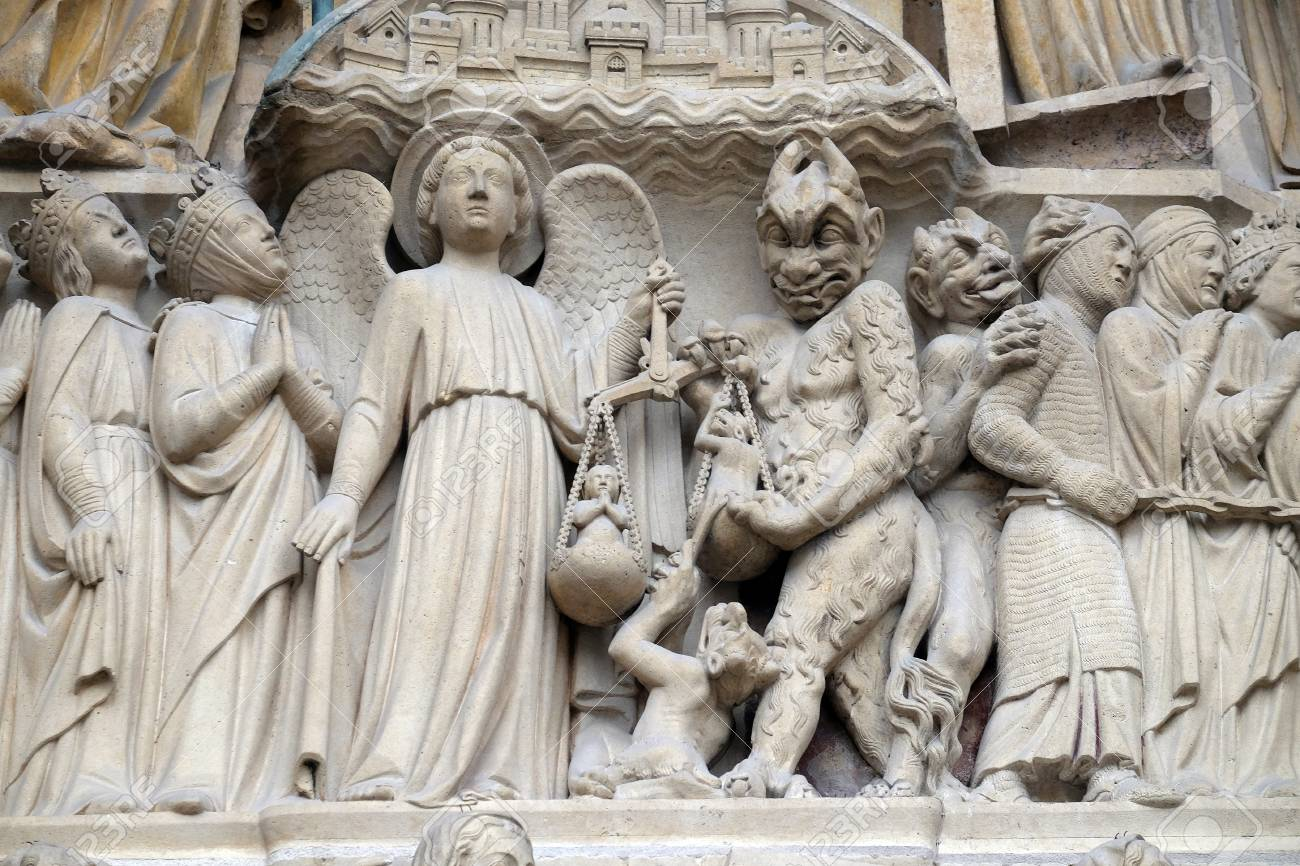
\includegraphics[width=0.85\linewidth]{image82.jpeg}
 \caption{6.2 Manuscritos Iluminados}
 \label{fig:cap14-img3}
\end{figure}

Tímpano ocidental de Notre-Dame de Paris (c. 1220) apresentando o Julgamento Final. Cristo Juiz aparece ao centro ladeado por instrumentos da Paixão, enquanto no registro inferior São Miguel pesa almas numa balança disputada com demônios. À direita de Cristo, os condenados são arrastados por correntes demoníacas em direção à boca do inferno representada como cabeça monstruosa devoradora - iconografia que deriva de tradições germânicas e celtas filtradas através da literatura visionária. Estas representações visuais funcionavam como "Bíblias de pedra" comunicando conceitos escatológicos a populações iletradas.

6.2 Manuscritos Iluminados


\begin{figure}[ht]
 \centering
 \includegraphics[width=0.85\linewidth]{image83.jpeg}
 \caption{7. Drama Medieval e Performance da Danação}
 \label{fig:cap14-img4}
\end{figure}

Representação do Inferno no Hortus Deliciarum de Herrad von Landsberg (c. 1180). A ilustração mostra uma das mais sistemáticas representações medievais do inferno, com diferentes categorias de pecadores sofrendo punições apropriadas supervisionadas por demônios especializados, combinando influências da Roda da Fortuna clássica com geografia infernal cristã.

Hortus Deliciarum de Herrad von Landsberg (c. 1180) apresenta representação sistemática: roda dividida em segmentos onde categorias de pecadores sofrem punições apropriadas supervisionadas por demônios especializados. Combina influências da Roda da Fortuna clássica com geografia infernal cristã.

7. Drama Medieval e Performance da Danação

Mystères e moralités francesas, dramatizações alemãs da Paixão, autos sacramentais ibéricos incorporam cenas infernais utilizando efeitos especiais (fogo, fumaça, machinery) criando experiências sensoriais de geografia infernal.

Mystères de la Passion (sécs. XIV-XV): Alçapões permitiam aparições de demônios; fogos de artifício simulavam chamas eternas; máscaras e fantasias criavam bestiário diabólico tridimensional.

O inferno dantesco resulta de extensas influências intelectuais e populares interculturais, criando visão multilayered única na literatura medieval, produto de rico diálogo entre civilizações.

A elaboração medieval de conceitos infernais estabelece paradigmas representacionais influenciando profundamente tradições posteriores. O Inferno dantesco torna-se referência fundamental desde Milton até cinema contemporâneo.

A síntese medieval continua informando imaginação ocidental sobre natureza do mal, justiça divina, e consequências escatológicas das escolhas morais, demonstrando vitalidade duradoura da síntese cultural medieval.

O período medieval representa momento culminante de criatividade teológica e artística integrando múltiplas tradições culturais numa visão compreensiva e sistemática do destino eterno humano. A Divina Comédia de Dante Alighieri emerge como síntese extraordinária que:

1. Integra tradições múltiplas: Cosmologia aristotélica, teologia tomista, geografia islâmica (Mi'raj), tradições visionárias cristãs, iconografia gótica, e intercâmbio cultural Al-Andalus.

2. Estabelece paradigmas duradouros: Sistema de contrapasso, geografia infernal estratificada, correspondências entre pecado e punição que influenciam representações subsequentes.

3. Reflete diálogo intercultural: Evidencias de transmissão através do Liber Scalae Machometi, paralelos estruturais com Mi'raj, influências místicas sufis demonstram rica interação entre civilizações.

4. Cria framework multicultural: Síntese única reconciliando tensões entre heranças culturais diversas, resultando em visão nuançada de justiça divina.

5. Influencia imaginação ocidental: Estabelece vocabulário visual e conceitual persistindo até o presente em literatura, arte, e cinema.

Esta realização intelectual e estética demonstra que as grandes obras culturais emergem de diálogo entre tradições, não de isolamento. A síntese dantesca exemplifica como o intercâmbio cultural enriquece expressão humana, criando monumentos artísticos que transcendem fronteiras temporais e geográficas.

O fascínio universal por questões do além-túmulo permitiu que muçulmanos e cristãos medievalmente compartilhassem visões sobre céu e inferno, anjos e demônios, destino da alma e justiça divina, deixando legado de influência mútua que continua informando pensamento religioso e imaginação cultural contemporâneos.

Bibliografia Selecionada


\section*{Fontes Primárias}
\addcontentsline{toc}{section}{Fontes Primárias}

Dante Alighieri. Divina Comédia. Ed. crítica Petrocchi.

Tomás de Aquino. Summa Theologica. Questões 69-70 (Suplemento).

Visio Tnugdali. Ed. crítica medieval.

Tractatus de Purgatorio Sancti Patricii. Fontes latinas.

Liber Scalae Machometi. Traduções medievais.


\section*{Fontes Secundárias}
\addcontentsline{toc}{section}{Fontes Secundárias}

Asín Palacios, Miguel. La Escatología musulmana en la Divina Comedia.

Barolini, Teodolinda. "Medieval Multiculturalism and Dante's Theology of Hell."

ELALAMI, A. "Eschatological Visions in Dante's Divine Comedy and the Abrahamic Traditions." Journal of Arts, Literature, Humanities and Social Sciences, 2025.

Casewit, Yousef. The Mystics of al-Andalus: Ibn Barrajān and Islamic Thought in the Twelfth Century. Cambridge, 2017.

Ebstein, Michael. Mysticism and Philosophy in al-Andalus: Ibn Masarra, Ibn al-'Arabī and the Ismā'īlī Tradition. Leiden, 2013.


% --- Capítulo 15: O Inferno na Renascença e na Reforma ---
\chapter[Renascença e Reforma]{O Inferno na Renascença e na Reforma}


\epigraph{O período da Renascença e Reforma representa transformação fundamental nas concepções sobre inferno e punição eterna, caracterizado por renovação humanística de fontes clássicas, controvérsias teológicas sobre salvação e escatologia, e emergência de sensibilidades artísticas que reinterpretam tradições medievais. Esta transformação, culminando nas decisões do Concílio de Trento e nas confissões protestantes, estabelece divergências doutrinárias que persistem até o presente.}

O humanismo renascentista aplica métodos filológicos para reinterpretar textos escatológicos, valorizando fontes originais e a análise patrística crítica. Pensadores como Lorenzo Valla e Erasmo de Rotterdam questionam elementos da geografia infernal medieval e o foco em punições sistemáticas. Além disso, a tradução dos clássicos, especialmente Platão por Marsílio Ficino, oferece novas alternativas filosóficas à escatologia aristotélico-tomista.

Martin Lutero (1483-1546) promoveu mudanças fundamentais na escatologia por meio das doutrinas de justificação pela fé e pela rejeição do purgatório. A remoção do purgatório como espaço intermediário de purificação modificou significativamente a estrutura da geografia escatológica, estabelecendo uma distinção mais acentuada entre salvação e condenação eterna. O conceito luterano de simul justus et peccator influenciou a compreensão sobre a condição humana e impactou interpretações acerca da justiça divina e do castigo eterno. A tradução da Bíblia para o vernáculo ampliou o acesso direto aos textos escatológicos, reduzindo a dependência em interpretações tradicionais eclesiásticas.

João Calvino (1509-1564) desenvolveu uma teologia sistemática que enfatiza a soberania divina e a dupla predestinação, segundo a qual alguns são eleitos para a salvação e outros para a danação. Essa visão determinista contrasta com o enfoque medieval na escolha moral e influenciou percepções sobre o destino eterno, gerando novas inquietações religiosas e artísticas sobre o inferno.

O Concílio de Trento (1545-1563) esclareceu a escatologia católica em resposta aos desafios protestantes, reafirmando crenças no purgatório, nas orações pelos mortos e nas indulgências. Suas decisões definiram as visões católicas sobre punição eterna e vida após a morte, distinguindo-as das perspectivas protestantes e influenciando posteriormente a arte e a literatura.

A arte renascentista introduziu técnicas inovadoras e reviveu a mitologia clássica para retratar o inferno. Artistas como Michelangelo (Capela Sistina) e Signorelli (Catedral de Orvieto) fundiram temas cristãos com imagens do submundo clássico, utilizando perspectiva avançada e conhecimento anatômico para criar cenas infernais mais realistas e emocionalmente impactantes.

O desenvolvimento da imprensa permitiu a ampla disseminação de textos e imagens escatológicas, criando um mercado de massa para obras que abordam morte, julgamento e destino eterno. Publicações renomadas como Ars Moriendi e diversos Livros de Horas passaram a alcançar públicos maiores, democratizando assim o acesso a conceitos escatológicos antes restritos à elite educada. Essa democratização moldou o entendimento popular e contribuiu para uma demanda por explicações mais acessíveis de ideias teológicas complexas sobre punição eterna.

O surgimento de estados confessionais após a Paz de Augsburgo (1555) introduziu dimensões políticas nas controvérsias escatológicas, em que conceitos de punição eterna passaram a ser marcadores tanto da identidade religiosa quanto política. O uso de imagens escatológicas na propaganda política e em polêmicas confessionais ilustra como os conceitos teológicos do inferno serviram a funções sociais e políticas que iam além dos contextos puramente religiosos.

Os desenvolvimentos científicos durante o Renascimento, especialmente a astronomia copernicana e a nascente filosofia natural, começaram a desafiar a cosmologia medieval, que fornecia a estrutura espacial para conceitos como o inferno. O deslocamento da Terra do centro do universo gerou questionamentos sobre a localização do inferno e de outros reinos escatológicos, debates esses que se intensificaram nos séculos seguintes. Esses desafios exigiram adaptações teológicas que iniciaram um processo de reinterpretar conceitos anteriormente entendidos em termos espaciais literais.

A expansão missionária que se seguiu à Era das Descobertas apresentou cristãos europeus a uma ampla variedade de tradições religiosas, cada uma com conceitos distintos sobre o pós-vida e punição. Esses encontros promoveram perspectivas comparativas que desafiaram pressupostos sobre a universalidade das ideias escatológicas cristãs. O contato com crenças indígenas americanas, africanas e asiáticas acerca da morte e do pós-vida levou a uma consideração mais profunda de como o contexto cultural influência as visões escatológicas, lançando as bases para interpretações mais relativistas nos séculos posteriores.

O período da Renascença e Reforma representou uma transformação fundamental nas concepções sobre inferno e punição eterna. Esse período foi caracterizado por uma renovação humanística das fontes clássicas, controvérsias teológicas sobre salvação e escatologia e a emergência de sensibilidades artísticas que reinterpretaram tradições medievais. Essa transformação -- culminando nas decisões do Concílio de Trento e nas confissões protestantes -- estabeleceu divergências doutrinárias que persistem até o presente.

Humanismo Renascentista e Reinterpretação da Escatologia

O humanismo renascentista aplicou métodos filológicos para reinterpretar textos escatológicos, valorizando as fontes originais e a análise patrística crítica. Filólogos como Lorenzo Valla e Erasmo de Rotterdam revisitaram os textos bíblicos e dos Padres da Igreja, questionando elementos da geografia infernal medieval e o foco em punições sistemáticas. Por exemplo, Erasmo ridicularizou em seus escritos certas crendices medievais sobre o inferno e enfatizou a necessidade de retornar ao significado genuíno das Escrituras. Além disso, a tradução de clássicos pagãos -- especialmente os diálogos de Platão, feita por Marsílio Ficino -- ofereceu novas alternativas filosóficas à escatologia aristotélico-tomista. Essa redescoberta do platonismo e de outras correntes antigas abriu espaço para imaginar a alma e o pós-vida de formas menos ligadas ao esquematismo escolástico medieval.


\section*{Críticas Pré-Reforma: Indulgências e Abusos da Igreja}
\addcontentsline{toc}{section}{Críticas Pré-Reforma: Indulgências e Abusos da Igreja}

Gravura renascentista ilustrando a venda de indulgências (Jörg Breu, c.1530). Os fiéis formam fila para comprar perdão, enquanto o dinheiro se acumula nos cofres da Igreja.
Na Baixa Idade Média, a Igreja Católica passou a conceder indulgências em troca de doações financeiras, permitindo aos pecadores a remissão das penas temporais devidas pelos pecados já confessados. Com o aumento do poder político e econômico do papado, essa prática descambou em abusos: a indulgência -- originalmente obtida por boas obras ou peregrinações -- tornou-se uma mercadoria negociada em dinheiro querobolsa.com.br. Sacerdotes e monges vendedores de indulgências (os quaestores) percorriam as regiões oferecendo “perdão garantido” em troca de pagamentos. O preço variava conforme a posição social do pecador e a gravidade do pecado; caso faltassem moedas, aceitavam-se terras, jóias, animais ou mesmo alimentos como pagamento querobolsa.com.br. Essa comercialização do sagrado enriqueceu a alta hierarquia eclesiástica, acumulando enormes riquezas e propriedades para a Igreja, mas gerou escândalo entre muitos cristãos. De fato, a Igreja detinha a maior concentração de riqueza na Europa no início do século XVI, muito dela oriunda da venda de indulgências iplimeira.com.br. Socialmente, essa prática difundiu a ideia de que era possível “comprar” a salvação, minando a genuinidade do arrependimento e provocando críticas de moralistas e humanistas. O próprio Erasmo de Rotterdam censurou os frades que pregavam indulgências, afirmando que aquilo parecia “nada além de uma transação comercial”en.wikipedia.org. Em suma, o impacto econômico das indulgências foi concentrar renda nas mãos da Igreja e do papado, enquanto seu impacto social foi alimentar a superstição popular e a revolta dos devotos conscientes.

As tensões causadas pelos abusos das indulgências e outros desvios (nepotismo, simonia, venda de relíquias sagradas etc.) formaram as bases para a Reforma Protestante. Diversos pensadores e movimentos pré-reformistas -- como John Wycliff na Inglaterra e Jan Hus na Boêmia -- já haviam condenado a corrupção e a avareza do clero, preparando o terreno intelectual para a ruptura. No início do século XVI, o descontentamento chegou a um ponto crítico: nobres e governantes se ressentiam de ver riquezas de seus territórios fluírem para Roma como reservas espirituais, e muitos fiéis comuns se indignavam com a exploração financeira de seus temores religiosos. Esse contexto explica por que, em 1517, a contestação de Martinho Lutero teve tanta ressonância: havia um anseio generalizado por moralização e mudança brasilescola.uol.com.br.

Martinho Lutero e a Redefinição da Escatologia Protestante

Martinho Lutero (1483--1546) promoveu mudanças teológicas profundas que repercutiram na escatologia cristã. Indignado com a “venda do perdão”, Lutero publicou suas famosas 95 Teses em 1517, nas quais criticava frontalmente o comércio de indulgências e a alegação de que o Papa teria poder de liberar almas do purgatório mediante pagamento pt.wikipedia.org. Um dos lemas atribuídos ao frade Johann Tetzel -- “Assim que uma moeda tilinta no cofre, uma alma sai do purgatório” -- exemplificava de forma crua essa teologia popular das indulgências pt.wikipedia.org. Lutero condenou tal ideia, argumentando que a salvação não estava à venda e somente Deus podia perdoar pecados, não um documento eclesiástico en.wikipedia.org. Para ele, as indulgências não garantiam a salvação de ninguém, servindo apenas para aumentar os lucros da Igreja en.wikipedia.org.

Em termos doutrinários, Lutero propôs a justificação pela fé somente (sola fide), rejeitando a noção de que obras ou penitências (como as indulgências) pudessem contribuir para a salvação. Com isso, ele também negou a existência do purgatório, espaço intermediário até então aceito pela teologia católica. Ao remover o purgatório da geografia escatológica, Lutero simplificou o destino pós-morte: restavam apenas céu e inferno, com uma distinção mais acentuada e definitiva entre salvação eterna e condenação eterna. Essa eliminação do purgatório abalou séculos de prática religiosa (visto que as indulgências, missas pelos mortos e orações de sufrágio perdiam sentido). Ademais, Lutero desenvolveu o conceito do cristão como simul justus et peccator (“simultaneamente justo e pecador”), enfatizando que mesmo os salvos permanecem pecadores dependentes da graça divina. Essa visão influenciou a compreensão da condição humana frente à justiça divina e, consequentemente, as ideias de punição eterna: o inferno, para Lutero, era merecido por todos os pecadores sem a graça de Cristo, e não havia “atalhos” sacramentais para escapar dele após a morte.

Outro aspecto crucial foi a tradução da Bíblia para o vernáculo (no caso de Lutero, para o alemão, em 1534). Ao verter as Escrituras para a língua do povo, Lutero democratizou o acesso aos textos escatológicos bíblicos -- como o Apocalipse e o Evangelho de Mateus (com suas parábolas sobre juízo final) -- reduzindo a dependência das interpretações eclesiásticas tradicionais. Milhares de leigos puderam ler diretamente as passagens sobre céu, inferno e juízo, o que fomentou discussões e entendimentos próprios acerca do destino eterno das almas. Em síntese, as reformas luteranas reconfiguraram radicalmente a escatologia: aboliram o purgatório, desacreditaram as indulgências e recentraram a questão da salvação na fé individual e na graça, moldando a visão protestante sobre inferno e punição eterna nos séculos seguintes.

João Calvino e a Escatologia da Predestinação

João Calvino (1509--1564), outro líder proeminente da Reforma, desenvolveu uma teologia sistemática que influenciou profundamente a concepção do destino eterno. Em suas obras -- sobretudo nas Institutas da Religião Cristã (1536) -- Calvino enfatizou a soberania absoluta de Deus e formulou a doutrina da dupla predestinação. Segundo essa doutrina, desde a eternidade Deus já havia eleito alguns para a salvação e destinado outros à danação, por Sua vontade soberana. Essa visão determinista contrastava com o enfoque medieval na escolha moral individual e no livre-arbítrio como fatores de salvação. Na prática, a teologia calvinista implicava que o inferno e o céu estavam predeterminados para cada alma, independentemente dos méritos ou ações humanas -- um pensamento que gerou novas inquietações religiosas e debates.

A ideia de que nem todos poderiam ser salvos, mas apenas os predestinados eleitos, levou a interpretações rigorosas da justiça divina e do papel das obras. Embora Calvino, assim como Lutero, negasse valor salvífico às indulgências e práticas similares, foi além ao estruturar uma visão coerente de escatologia baseada na predestinação. O inferno, nessa perspectiva, era parte do decreto divino, existindo para manifestar a justiça de Deus contra o pecado dos réprobos. Essa teologia calvinista influenciou enormemente a mentalidade religiosa nas regiões reformadas (como Suíça, Holanda, Escócia), incutindo um senso austero de responsabilidade moral pessoal e, ao mesmo tempo, de resignação quanto aos insondáveis desígnios divinos sobre o destino eterno. Artistas e escritores influenciados pelo calvinismo frequentemente retrataram o inferno como algo terrível porém justo, reservado aos que Deus não escolhera salvar -- uma abordagem notável, distinta tanto do medievalismo católico quanto de outras vertentes protestantes mais voltadas ao livre-arbítrio.

O Concílio de Trento e a Resposta Católica

O Concílio de Trento (1545--1563) marcou a resposta da Igreja Católica à Reforma e trouxe importantes definições escatológicas. Confrontada com os desafios protestantes, a Igreja reafirmou doutrinas tradicionais como a existência do purgatório, a eficácia das orações pelos mortos e a validade das indulgências -- demarcando claramente as diferenças em relação às novas confissões protestantes. Trento, porém, reconheceu a necessidade de reforma interna. Sobre as indulgências, em particular, o Concílio condenou os abusos financeiros envolvidos na prática. No decreto de 16 de julho de 1562, determinou-se que na concessão de indulgências deveria haver moderação e que “todo ganho ilícito associado a ela seja completamente abolido, como uma grave corrupção entre os fiéis”pt.wikipedia.org. Os bispos passaram a ter a obrigação de supervisionar e eliminar eventuais práticas abusivas de perdão vendido em suas dioceses pt.wikipedia.org. Assim, embora Trento tenha mantido o princípio teológico das indulgências (ligado à ideia de um “tesouro de méritos” dos santos aplicado pela Igreja), procurou coibir a exploração comercial que motivara tantas críticas. De fato, após o Concílio, a venda aberta de indulgências praticamente cessou -- as indulgências continuaram a existir, mas vinculadas a penitências e atos devocionais, não a transações monetárias.

Em matéria de inferno e salvação, o Concílio de Trento reafirmou a posição católica tradicional: a salvação envolve fé e obras (contra o sola fide protestante), o inferno é real e eterno para os que morrem em pecado mortal, e o purgatório permanece como estado temporário de purificação para os salvos imperfeitos. Ao definir esses pontos, a Igreja Católica solidificou sua escatologia “oficial” em contraste com as visões reformadas. Essas definições influenciariam a arte e a literatura católicas pós-Trento -- por exemplo, a ênfase no purgatório e na oração de intercessão pelos mortos aparece em inúmeras pinturas, sermões e hinos do período barroco. Em suma, o Concílio de Trento funcionou como um divisor de águas: consolidou os ensinamentos tradicionais sobre inferno, purgatório e salvação, ao mesmo tempo em que implementou reformas disciplinares para restaurar a credibilidade da Igreja frente às críticas justificadas sobre corrupção e indulgências.


\section*{Arte Renascentista: Novas Visões do Inferno}
\addcontentsline{toc}{section}{Arte Renascentista: Novas Visões do Inferno}

A arte renascentista também refletiu a transformação nas concepções de inferno e punição. Artistas do alto Renascimento introduziram técnicas inovadoras de perspectiva e anatomia, além de incorporar influências da mitologia clássica greco-romana, para retratar o inferno e o juízo final de maneiras mais realistas e emocionalmente impactantes. Um exemplo notável é a obra de Luca Signorelli na Catedral de Orvieto (1499--1504), onde afrescos do Juízo Final mostram demônios, corpos nus e tormentos infernais com um detalhismo anatômico impressionante para a época. Em Roma, Michelangelo Buonarroti, ao pintar o Juízo Final na Capela Sistina (1536--1541), quebrou com representações tradicionais: em vez de dispor as figuras em faixas horizontais separando céu, terra e inferno, ele criou uma composição dinâmica e circular, com Cristo no centro irradiando luz como um “sol” justo. Alguns estudiosos sugerem que Michelangelo pode ter sido influenciado pelas ideias heliocêntricas de Copérnico ao conceber essa cena centralizada em Cristo-Solgresham.ac.ukgresham.ac.uk -- embora De revolutionibus só tenha sido publicado dois anos depois de concluído o afresco, a concepção “cósmica” da obra é evidente. O inferno de Michelangelo aparece na parte inferior do afresco, mas integrado num movimento circular que envolve todo o cenário, enfatizando a interconexão do destino das almas.

Além desses mestres, toda uma geração de artistas renascentistas reinterpretou visualmente as penas eternas. As influências clássicas levaram a comparações entre o Hades pagão e o inferno cristão. Motivos da mitologia -- como o julgamento das almas por Minos ou Caronte conduzindo as almas no barqueiro infernal -- surgem em obras de fine arts do período, mesclados com a teologia cristã. Essa fusão iconográfica resulta em imagens infernais de grande vigor dramático: monstros e demônios foram pintados com base no estudo científico de animais exóticos (ou das grotescas figuras mitológicas), enquanto os corpos dos condenados foram retratados com conhecimento de anatomia humana sem precedentes, conferindo alto grau de realismo às cenas de tortura e desespero. O resultado foram obras que chocavam e ao mesmo tempo catequizavam o público, tornando tangível o destino temível dos pecadores. Em última análise, a arte renascentista do inferno serviu tanto para expressar as ansiedades escatológicas de uma era de mudança quanto para comunicar as doutrinas (católicas ou protestantes) a um público mais amplo, muitas vezes analfabeto, através do poder vívido das imagens.

A Imprensa e a Popularização das Ideias Escatológicas

A invenção da imprensa de tipos móveis por Johannes Gutenberg (por volta de 1450) e seu aperfeiçoamento ao longo do século XVI permitiram uma ampla disseminação de textos e imagens escatológicas, transformando a cultura religiosa europeia. Antes, obras sobre o além (tratados teológicos, visões místicas, ilustrações do inferno) circulavam de forma limitada, principalmente em manuscritos caros acessíveis à elite eclesiástica. Com a imprensa, títulos populares como o Ars Moriendi (“Arte de Morrer Bem”) -- manual que ensinava os leigos a enfrentar a morte e a tentação final -- passaram a ser produzidos em massa e em diversas línguas vernaculares. Do mesmo modo, os Livros de Horas (devocionários ricamente ilustrados com cenas do Juízo Final e do inferno) deixaram de ser exclusivos dos nobres para ganhar versões simplificadas e baratas para a burguesia urbana. Essa democratização do acesso moldou o entendimento popular da escatologia: pessoas comuns puderam visualizar e ler sobre os horrores do inferno e as bem-aventuranças do céu por si mesmas, sem depender integralmente dos sermões.

Impressos panfletários também tiveram grande importância. Por exemplo, durante as controvérsias da Reforma, panfletos ilustrados de ambos os lados faziam caricaturas escatológicas: protestantes mostravam o Papa e os cardeais caminhando rumo ao inferno carregados de riquezas (numa crítica às indulgências), enquanto católicos imprimiam folhetos alertando que os hereges reformadores levariam as almas dos incautos à danação. Essas imagens, de fácil compreensão, espalhavam propaganda religiosa usando o medo do inferno como retórica persuasiva. Além disso, a possibilidade de imprimir a Bíblia em línguas vernáculas (como já citado no caso de Lutero) e difundi-la em larga escala revolucionou a formação espiritual dos europeus: o Apocalipse de São João, com seus vívidos cenários de julgamento e lago de fogo, tornou-se um dos livros mais lidos, inspirando desde pregadores apocalípticos até artistas como Albrecht Dürer (que ilustrou o Apocalipse em xilogravuras famosas de 1498). Em resumo, a imprensa criou um mercado de massa para temas escatológicos, levando conceitos antes eruditos -- como purgatório, indulgências, fim dos tempos -- ao imaginário popular e preparando o terreno para a efervescência religiosa do século XVI.

Estados Confessionais e Propaganda do Inferno

Após as reformas religiosas, sobretudo com a Paz de Augsburgo (1555) que legalizou o luteranismo no Sacro Império, surgiram os estados confessionais na Europa (territórios definidos por uma confissão religiosa oficial, católica ou protestante). Nesses estados, as diferenças teológicas sobre salvação e condenação eterna passaram a ter também uma função política e identitária. Conceitos de punição eterna tornaram-se marcadores não apenas de filiação religiosa, mas de lealdade cívica. Por exemplo, em principados alemães luteranos, a figura do Papa às vezes era públicamente associada ao Anticristo apocalíptico que levaria as almas ao inferno -- uma forma de consolidar a identidade protestante local em oposição a Roma. Do lado católico, a Contra-Reforma usou o medo do inferno para reafirmar a autoridade da Igreja: missionários jesuítas pregavam com vigor sobre as penas eternas que aguardavam hereges e apóstatas, enquanto artistas barrocos (como no ciclo de pinturas da Igreja do Gesù, em Roma) mostravam vívidas cenas de pecadores sendo lançados no fogo como advertência ao público.

A propaganda política daquele tempo frequentemente empregou imagens escatológicas. Folhetos de guerra, por exemplo, podiam retratar os inimigos -- fosse a facção protestante ou católica contrária -- sofrendo tormentos infernais como forma de desumanizá-los e justificar conflitos. Em países como a Inglaterra elisabetana (anglicana) e a França durante as guerras religiosas, panfletos circularam demonizando minorias religiosas internas (católicos na Inglaterra, huguenotes na França) e associando-as a condenação eterna. Assim, o inferno deixou de ser apenas um conceito teológico distante para se tornar uma arma retórica imediata na política europeia do século XVI. Esse uso político do inferno e do apocalipse evidenciou que os conceitos teológicos do pós-vida serviam a funções sociais e políticas, dando coesão a comunidades, justificando autoridade e marginalizando opositores. As divergências doutrinárias entre confissões -- se existia ou não purgatório, se a salvação era predestinada ou acessível a todos, se santos intercediam pelas almas, etc. -- delinearam fronteiras não apenas religiosas mas também nacionais e culturais, cujos ecos permanecem visíveis em atitudes e identidades até hoje.

Revolução Científica e Questionamentos Cosmológicos

O século XVI foi não apenas de revoluções religiosas, mas também o limiar de uma revolução científica que desafiaria antigas concepções do cosmos -- e, com elas, certas bases da geografia escatológica medieval. Em 1543, Nicolau Copérnico publicou De revolutionibus orbium coelestium, obra que propunha o modelo heliocêntrico do universo (com o Sol no centro e a Terra girando ao redor)ncse.ngoncse.ngo. Essa ideia, ilustrada por Copérnico em diagramas astronômicos revolucionários commons.wikimedia.org, desmontava o esquema tradicional herdado de Ptolomeu e Aristóteles, no qual a Terra imóvel ocupava o centro do cosmos e os reinos espiritual e material estavam rigidamente ordenados em esferas concêntricas -- com Deus e os bem-aventurados nos céus mais elevados e o inferno literalmente localizado nas profundezas ou no centro da Terra. Antes de Copérnico, a cosmologia escolástica integrava teologia e astronomia a ponto de “governar desde a natureza da matéria e movimento planetário até a localização geográfica do céu e do inferno”ncse.ngo. Por exemplo, na Divina Comédia de Dante (1320), o inferno é uma caverna física no miolo do globo terrestre, exatamente no centro do universo geocêntrico.

A descentralização da Terra trazida pelo heliocentrismo Copernicano teve consequências inquietantes para esse imaginário: se o planeta não era mais o centro fixo da criação, onde ficariam agora o inferno (tradicionalmente concebido “embaixo” da Terra) e mesmo o céu (antes visualizado nas esferas acima das estrelas fixas)? Já em meados do século XVI e início do XVII, alguns pensadores perceberam essas implicações. A princípio, a Igreja Católica reagiu com cautela -- Copérnico dedicara sua obra ao Papa e apresentou seu modelo como hipótese matemática. Entretanto, conforme os avanços científicos se acumulavam (as observações de Galileu com a luneta em 1610, as leis de Kepler etc.), a cosmologia medieval começou a ruir. Teólogos foram desafiados a reinterpretar os conceitos escatológicos de forma menos literal e espacial. Por exemplo, o astrônomo jesuíta Giovanni Riccioli, em 1651, considerou e descartou a objeção de que, num universo heliocêntrico, faltaria um lugar para o inferno: ele argumentou que o inferno não precisava ser um lugar físico determinado para existir como realidade teológicathonyc.wordpress.com. Declarações assim iniciaram um processo de “desmaterialização” do inferno -- de um local geográfico palpável para uma condição espiritual de separação de Deus.

Esse choque entre nova ciência e antigas crenças culminou em eventos dramáticos, como o julgamento de Galileu Galilei em 1633, no qual a Inquisição condenou a defesa do heliocentrismo por aparentemente contradizer as Escrituras (que falavam, por exemplo, de um Sol que “para” no céu em Josué 10:13). Ainda que a questão central fosse astronômica, em sentido mais amplo estava em jogo a autoridade interpretativa da Igreja sobre questões do cosmos e, por extensão, do céu e inferno. Ao longo dos séculos seguintes, a Igreja gradualmente acomodou as descobertas científicas (aceitando o heliocentrismo e outras teorias), e com isso a visão do inferno como uma caverna ardente dentro da Terra cedeu lugar a concepções mais abstratas ou metafísicas de inferno -- um “estado” de alma separado de Deus, não necessariamente um espaço com coordenadas geográficas. Em retrospecto, a Revolução Copernicana contribuiu para a secularização da visão de mundo, removendo o homem e seu planeta do centro do universo e relativizando as preocupações humanas diante das “infinitudes do tempo e do espaço”ncse.ngo. A teologia cristã, instigada por esses desenvolvimentos, teve que refinar a escatologia: o céu e o inferno tornaram-se menos objetos de mapas e mais de reflexão ética e espiritual, mantendo-se como realidades de fé, porém entendidas de forma compatível com um universo infinito e governado por leis naturais.

Descobrimentos Geográficos e Relativização Cultural da Escatologia

Por fim, outro fator que moldou as concepções de inferno e punição eterna na Renascença e Reforma foi a expansão missionária e os contatos interculturais decorrentes da Era dos Descobrimentos. Nos séculos XV e XVI, navegadores europeus alcançaram as Américas, dobraram o Cabo da Boa Esperança rumo à Ásia e estabeleceram colônias e postos de comércio na África e no Oriente. Esses encontros colocaram os cristãos europeus em contato com uma grande diversidade de religiões e cosmologias. Populações indígenas da América tinham suas próprias ideias sobre o pós-vida (como as concepções astecas de um inframundo multilayer, ou as crenças tupis em espíritos ancestrais); da mesma forma, na Ásia encontraram-se tradições como o budismo, que concebia ciclos de reencarnação e estados de purgação (naraka, análogo ao inferno), e o hinduísmo, com seus castigos kármicos e mundos inferiores habitados por entidades demoníacas.

Essas comparações forçadas levaram missionários e teólogos a uma perspectiva mais relativista sobre o inferno: perceberam que a noção de punição pós-morte não era exclusiva do cristianismo, nem mesmo homogênea dentro dele. Relatos de jesuítas, como os de São Francisco Xavier no Japão ou de José de Anchieta no Brasil, descreviam as crenças locais e muitas vezes tentavam encontrar pontes de entendimento -- por exemplo, equiparando de forma simplificada o inferno cristão ao Xibalba maia, ou identificando certos deuses pagãos com demônios bíblicos. Enquanto alguns usaram as semelhanças para facilitar a evangelização (afirmando que, no fundo, todos os povos tinham um senso inato de justiça pós-vida que o cristianismo vinha aperfeiçoar), outros pensadores europeus começaram a questionar se as imagens tradicionais de inferno não teriam também elas um componente cultural. Afinal, se povos “pagãos” possuíam visões de tormento eterno, o que garantiria que a compreensão europeia medieval não estivesse igualmente influenciada por imaginação e contexto?

Assim, nos séculos posteriores (XVII e XVIII), ganha força na Europa uma postura mais crítica e ilustrada, que reavalia doutrinas como a do inferno eterno à luz da razão e da experiência universal. Já no fim do XVI, Michel de Montaigne escrevia sobre a diversidade de crenças em diferentes culturas para relativizar certezas europeias. No campo escatológico, esse processo plantou as sementes para correntes teológicas mais liberais ou simbólicas quanto ao inferno (como o universalismo, que negaria a eternidade das penas, ou interpretações alegóricas do fogo do inferno). Em suma, os Descobrimentos e a missão ultramarina diluíram a convicção na universalidade de uma só narrativa escatológica. Embora no curto prazo o efeito tenha sido reforçar o zelo missionário (para salvar almas “pagãs” do inferno), no longo prazo levou a cristandade a encarar suas imagens do além com maior consciência de contexto histórico e cultural, pavimentando o caminho para debates teológicos modernos sobre a natureza da punição eterna.

O Renascimento e a Reforma foram uma era de transição vertiginosa, em que a visão ocidental do inferno e da punição eterna foi questionada e redesenhada em múltiplos níveis -- filológico, teológico, artístico, científico e cultural. Da filologia humanista que depurou exageros medievais, passando pelas reformas protestantes que aboliram o purgatório e denunciaram a comercialização da salvação, até os ajustamentos católicos pós-Trento e o confronto com novos mundos e novos céus, todas essas forças contribuíram para uma renovação escatológica. Ao final do período, a cristandade encontrava-se dividida em distintas tradições doutrinárias, cada qual com sua compreensão do inferno (seja como fogo eterno literal ou metáfora da separação divina, com ou sem estágio purgatório, com pena igual para todos os condenados ou graus de punição etc.). Essas divergências estabelecidas no século XVI persistem, de forma adaptada, até o presente -- lembrete de como aquele momento histórico moldou profundamente a imaginação religiosa acerca do destino final da alma humana. As decisões conciliares católicas e as confissões de fé protestantes fixaram parâmetros que ainda hoje norteiam o debate sobre justiça divina e misericórdia, enquanto as inquietações científicas e culturais iniciadas então continuaram a provocar reflexões e ajustes na maneira de entender realidades últimas como o céu e o inferno. Em síntese, a Renascença e a Reforma legaram-nos não apenas conflitos e divisões, mas também um legado rico de diálogo crítico sobre o além -- um diálogo que enriqueceu a teologia e desafia continuamente cada geração a reconsiderar o que realmente significam inferno, punição e esperança de eternidade.

Referências:

BÍBLIA. Ars Moriendi, Livros de Horas e outros impressos devocionais. Mainz: s.n., c.1500.

querobolsa.com.br Querobolsa. Indulgências: o que eram, venda e significado. Acesso em 09 nov. 2025.

querobolsa.com.br Querobolsa. Indulgências: o que eram, venda e significado. Detalhes sobre a venda de indulgências por valores materiais.

en.wikipedia.org Wikipedia (en). Indulgence -- Protestant Reformation. Citação da tese de Lutero contra venda da salvação: “assim que a moeda...”.

en.wikipedia.org Wikipedia (en). Indulgence -- Protestant Reformation. Lutero denunciando o ganho e cobiça por trás das indulgências.

en.wikipedia.org Wikipedia (en). Indulgence -- Erasmus’s critique. Erasmo de Rotterdam criticando abusos das indulgências como “transação comercial”.

thonyc.wordpress.com Renaissance Mathematicus. Science contra Copernicus. Referência a Riccioli descartando objeção sobre localização do inferno no heliocentrismo.

gresham.ac.ukgresham.ac.uk Gresham College. Michelangelo, Copernicus and the Sistine Chapel. Discussão sobre influência heliocêntrica no Juízo Final de Michelangelo.

pt.wikipedia.org Wikipedia (pt). Indulgência -- Abusos. Referência à frase de Tetzel: “moeda tilinta no cofre...”.

pt.wikipedia.org Wikipedia (pt). Indulgência -- Reforma Protestante. Papa Leão X vendendo indulgência para São Pedro e reação de Lutero (95 Teses).

pt.wikipedia.org Wikipedia (pt). Indulgência -- Concílio de Trento. Decreto tridentino sobre moderação e fim dos ganhos ilícitos com indulgências.

ncse.ngo NCSE. Copernicus: No Friend to Biblical Literalists. Integração do cosmos medieval com localização de céu e inferno.

ncse.ngo NCSE. Copernicus: No Friend to Biblical Literalists. Remoção da Terra do centro e implicações para teologia (secularização, relativização).

brasilescola.uol.com.br Brasil Escola. Reforma Protestante -- causas. Indignação de Lutero com venda de indulgências por Leão X.

brasilescola.uol.com.br Brasil Escola. Reforma Protestante -- causas. Apoio de nobres pela oportunidade de autonomia política e econômica (fim de impostos à Igreja).

iplimeira.com.br IP Limeira. Consequências da Reforma -- Economia. Igreja possuía maior riqueza, oriunda da venda de indulgências, antes da Reforma.

iplimeira.com.br IP Limeira. Consequências da Reforma -- Economia. Nas regiões protestantes, redistribuição do capital da Igreja para cidades e estados após a Reforma.


% --- Capítulo 16: O Inferno no Iluminismo ---
\chapter[O Inferno no Iluminismo]{O Inferno no Iluminismo}


\epigraph{O período do Iluminismo marca transformação radical nas concepções sobre inferno e punição eterna, caracterizado pela emergência da crítica histórica, racionalização filosófica dos conceitos religiosos, e desenvolvimento de perspectivas seculares sobre moralidade e justiça. Esta transformação, acelerada pela Revolução Científica e mudanças sociais associadas à modernização, estabelece tensões entre tradições religiosas herdadas e sensibilidades modernas que persistem até o presente.}

A crítica histórica desenvolvida por figuras como Richard Simon (1638-1712) e Jean Astruc (1684-1766) introduz metodologias que questionam origens e desenvolvimento de textos bíblicos escatológicos, estabelecendo precedentes para análise científica de conceitos religiosos. A aplicação de princípios histórico-críticos a documentos bíblicos identifica estratificações temporais e influências culturais na formação de conceitos sobre inferno, questionando interpretações literais tradicionais e sugerindo abordagens hermenêuticas alternativas. O deísmo iluminista, exemplificado por Voltaire e Hume, contesta a punição eterna ao defender que uma divindade benevolente é incompatível com tal castigo. Essa crítica racional impulsionou reflexões teológicas sobre a natureza e duração da punição eterna.

Immanuel Kant (1724-1804) revolucionou a filosofia moral por meio do imperativo categórico e da ênfase na autonomia, influenciando as visões sobre justiça e punição. Ele questionou a justiça de um castigo eterno para faltas finitas, instando a teologia filosófica a considerar a dignidade humana em relação à justiça divina.

A gradual secularização da cultura europeia durante os séculos XVII e XVIII estabeleceu contextos em que os conceitos escatológicos perderam imediatismo na vida cotidiana, transformando assim a noção de inferno de uma realidade urgente para uma metáfora cultural. Essa mudança é particularmente evidente na literatura, onde a imagem infernal passa a funcionar cada vez mais como instrumento de crítica psicológica e social, em vez de servir como advertência escatológica literal. O declínio na crença em punição eterna literal correlaciona-se com o surgimento de sistemas seculares de moralidade e justiça.

Avanços científicos, especialmente em geologia e cosmologia, desafiaram as concepções espaciais tradicionais do inferno através de descobertas relacionadas ao tempo profundo e às vastas escalas do universo. Evidências geológicas sobre a idade da Terra e achados astronômicos acerca da dimensão do cosmos tornaram localizações convencionais do inferno menos plausíveis, exigindo adaptações teológicas que espiritualizaram interpretações antes literais. Esse processo de espiritualização marca uma transformação significativa na compreensão escatológica.

O surgimento da religião comparada como disciplina acadêmica no século XIX introduziu o estudo sistemático de diversas tradições escatológicas, revelando tanto padrões comuns quanto variações distintas na punição pós-morte entre culturas. As obras de estudiosos como Max Müller (1823--1900) e James Frazer (1854--1941) destacam a universalidade das preocupações escatológicas e, ao mesmo tempo, salientam especificidades culturais referentes aos conceitos de punição eterna.

A psicologia emergente, principalmente por meio do trabalho de Sigmund Freud (1856--1939), apresenta explicações naturalistas para a crença na punição eterna através de noções como culpa, repressão e projeção. Interpretações psicanalíticas mostram a crença escatológica como expressão de processos psicológicos inconscientes, oferecendo estruturas alternativas para compreender o apelo persistente da punição eterna mesmo em sociedades cada vez mais seculares.

A revolução industrial e as mudanças sociais associadas geraram novos contextos para interpretar sofrimento e injustiça, moldando a compreensão sobre punição eterna. Experiências de pobreza urbana, acidentes industriais e deslocamento social forneceram exemplos imediatos de sofrimento sistêmico, tornando as explicações teológicas de justiça divina mais problemáticas e contribuindo para o declínio das crenças escatológicas tradicionais.

O protestantismo liberal surgiu como resposta aos desafios modernos, desenvolvendo abordagens teológicas que enfatizavam o amor divino em detrimento da justiça divina e influenciando concepções de punição eterna em direção ao universalismo e à imortalidade condicional. Pensadores influentes como Friedrich Schleiermacher (1768--1834) formularam doutrinas que buscavam reconciliar ensinamentos cristãos tradicionais com sensibilidades contemporâneas sobre dignidade humana e compaixão divina, criando assim tradições escatológicas alternativas que persistem até os dias atuais.

1. Crítica Histórica e Autoridade Religiosa: O Iluminismo inaugurou abordagens críticas aos textos sagrados que abalaram a autoridade religiosa tradicional sobre doutrinas como o inferno e a punição eterna. Eruditos como Richard Simon (1638--1712) e Jean Astruc (1684--1766) aplicaram métodos histórico-críticos à Bíblia, revelando múltiplas fontes e camadas temporais nos textos escatológicos. Essa análise evidenciou influências culturais e editores humanos na formação de passagens sobre o inferno, minando leituras literalmente infalíveis e demonstrando que conceitos de punição pós-morte evoluíram historicamente em vez de terem sido revelados de uma vez por todas. A divulgação desses estudos -- muitas vezes enfrentando censura e resistência eclesiástica -- dessacralizou as Escrituras, pois expôs incoerências e inserções tardias antes aceitas sem questionamento secularhumanism.org. Ao tratar criticamente os ensinamentos religiosos, o Iluminismo reduziu o medo do inferno como ferramenta de controle social e desafiou o monopólio hermenêutico das igrejas sobre o destino das almas. Em suma, a crítica histórica abriu caminho para leituras mais metafóricas ou éticas das noções de inferno, retirando delas a aura de dogma intocável e sujeitando-as à verificação racional e ao contexto histórico.

2. Racionalismo Filosófico e Teorias de Justiça: Filósofos iluministas e deístas questionaram a coerência moral da doutrina do inferno eterno, influenciando o pensamento político-jurídico sobre justiça e punição. Pensadores como Voltaire e David Hume argumentaram que atribuir crueldade infinita a um Deus benevolente era ilógico, pondo em xeque a ideia de um castigo eterno incompatível com a misericórdia divina. Essa crítica racional ressaltou a desproporção entre pecados finitos e tormento infinito, introduzindo o princípio iluminista de proporcionalidade das penas também no discurso teológico. O imperativo categórico de Immanuel Kant (1724--1804), com sua ênfase na autonomia e dignidade humanas, reforçou essas indagações: Kant considerou injusto punir transgressões limitadas com sofrimentos sem fim, o que instou teólogos a repensarem a justiça divina em termos compatíveis com a razão moral humana. A filosofia política da época igualmente repudiava punições excessivamente severas -- Cesare Beccaria, em Dos Delitos e das Penas (1764), defendeu punições úteis e comedidas em vez de suplícios brutais webpages.cs.luc.edu. Tal humanitarismo legal contrastava fortemente com a visão medieval do inferno como tortura eterna, tornando essa última cada vez mais ética e emocionalmente insustentável. Além disso, autores como Paul d’Holbach radicalizaram o secularismo moral: ele pregava que os homens deviam evitar crimes “não porque serão punidos no outro mundo, mas porque sofrerão por isso neste”webpages.cs.luc.edu. Esse deslocamento do foco punitivo para as consequências terrenas exemplifica como o Iluminismo substituiu o temor do inferno por princípios laicos de ética e justiça, abalando a legitimidade da punição eterna na cultura intelectual.

3. Secularização da Sociedade e Mudanças Socioeconômicas: A progressiva secularização europeia nos séculos XVII e XVIII transformou profundamente a maneira como o inferno era concebido, retirando-o do centro das preocupações cotidianas e ressignificando-o em contextos culturais e políticos emergentes. À medida que a tolerância religiosa e a separação entre Igreja e Estado ganhavam espaço como ideais iluministas pt.wikipedia.org, a crença literal em Satanás, milagres e no fogo do inferno enfraqueceu visivelmente entre os pensadores educados cdn.vanderbilt.edu. O resultado foi que o inferno deixou de ser uma ameaça iminente garantida pela autoridade do clero e passou a ser frequentemente reinterpretado como metáfora moral ou literária. Autores da época -- principalmente na Inglaterra vitoriana e na França pós-revolucionária -- empregaram imagens infernais para criticar vícios sociais e estados psicológicos, em vez de como advertência teológica. Paralelamente, avanços científicos solaparam as bases cosmológicas do inferno tradicional: descobertas em geologia (tempo geológico profundo) e astronomia (vastidão do universo) tornaram geograficamente implausível a noção de um inferno físico localizado no interior da Terra ou nos confins do cosmos. Em resposta, muitas correntes religiosas espiritualizaram o inferno, passando a defini-lo não como um lugar de fogo material, mas como um estado de afastamento de Deus ou de angústia da consciência -- uma mudança conceitual significativa motivada pelo novo conhecimento científico e pela mentalidade secular.

Pintura Coalbrookdale by Night (1801) de P. J. de Loutherbourg, retratando fornalhas acesas na Inglaterra industrial -- um símbolo artístico do “inferno” associado às paisagens fabris do período. Durante a Revolução Industrial, as dramáticas mudanças econômicas e urbanas forneceram novos prismas para entender o sofrimento e a injustiça, moldando a imaginação escatológica. As cidades industriais superlotadas, envoltas em poluição e marcadas por trabalho extenuante, foram descritas por observadores como “infernos na Terra”, refletindo a substituição de terrores ultramundanos por críticas sociais terrenas thehumandivine.org. Escritores e artistas (como William Blake em suas ilustrações da Divina Comédia) usaram a iconografia infernal para denunciar as condições desumanas enfrentadas pelo proletariado nascente, sugerindo que o verdadeiro inferno podia manifestar-se nos bairros operários e fábricas insalubres. Essa sensibilização para os males sistêmicos -- pobreza urbana, acidentes laborais, exploração do trabalho infantil -- enfraqueceu a eficácia de explicações teológicas simplistas que viam sofrimento apenas como punição divina ao pecado individual. Em vez disso, fomentou-se a noção de que cabia à sociedade (e não ao fogo eterno) corrigir tais injustiças. Desse modo, a modernização econômica e os novos problemas sociais reduziram ainda mais a aderência à doutrina tradicional do inferno, ao mesmo tempo em que a imagem do inferno se secularizou como crítica sociopolítica e não mais como destino certo dos descrentes.

4. Perspectivas Religiosas Modernas e Legados Contemporâneos: Os séculos XIX e XX aprofundaram a transformação do conceito de inferno, incorporando tanto análises comparativas de religiões quanto novas abordagens teológicas influenciadas por valores políticos contemporâneos. O surgimento da Religião Comparada como disciplina acadêmica (com pioneiros como Max Müller e James Frazer) revelou que quase todas as culturas possuíam algum conceito de punição pós-morte, porém variando em duração e propósito. Esse estudo comparativo ressaltou paralelos entre o inferno cristão e mitologias de outras tradições, relativizando a noção de punição eterna como algo possivelmente simbólico ou cultural, em vez de uma verdade exclusiva. Simultaneamente, a Psicologia da Religião ofereceu explicações naturalistas para a persistência da crença no inferno. Sigmund Freud (1856--1939), por exemplo, interpretou o medo do inferno e a culpa religiosa como projeções do inconsciente -- produtos de ansiedade moral reprimida e do superego --, sugerindo que o “fogo eterno” exerce uma função psicológica (controle pelo medo) mais do que corresponde a uma realidade objetiva. Essa visão reduziu o inferno ao âmbito da mente humana, ecoando o dito de Sartre de que “o inferno são os outros” ou mesmo nós mesmos, ao invés de um lugar físico de chamas. Em resposta a essas influências e aos dilemas éticos do mundo moderno, muitas correntes cristãs adotaram posturas teológicas mais liberais. O protestantismo liberal dos séculos XIX-XX -- com expoentes como Friedrich Schleiermacher (1768--1834) -- reelaborou a doutrina escatológica enfatizando o amor e a misericórdia divinos em detrimento da ira punitiva. Schleiermacher, em particular, abraçou o universalismo por não conseguir reconciliar um Deus amoroso e soberano com a existência do inferno paleoortodoxo.com. Ele argumentou que, se Deus é perfeitamente bom e governa todas as coisas, não faz sentido crer que destinaria Suas criaturas a tormento sem fim; um Criador justo providenciaria antes ou a salvação de todos ou a extinção misericordiosa dos irremediavelmente maus. Ideias assim pavimentaram o caminho para doutrinas alternativas como o Universalismo (salvação eventual de todos) e a Imortalidade Condicional (os ímpios deixariam de existir em vez de sofrer eternamente), que ganharam força entre teólogos e pensadores religiosos. Essa tendência se manifestou em várias denominações cristãs ao longo do século XX, marcada também por reconsiderações do inferno dentro da Igreja Católica (por exemplo, a visão do inferno como “autoexclusão” do amor de Deus, conforme desenvolvida no Concílio Vaticano II). No conjunto, tais abordagens reformistas buscaram alinhar a escatologia com os ideais humanitários modernos, reconhecendo a dignidade humana e a repulsa moral que a ideia de suplício infinito desperta. Assim, do Iluminismo em diante, o conceito de punição eterna foi sendo gradualmente amenizado ou abandonado em muitos círculos religiosos, dando lugar a interpretações mais compatíveis com a sensibilidade contemporânea. Essa revisão multidisciplinar -- histórica, científica, psicológica e teológica -- do inferno eliminou em grande medida seu caráter literal aterrorizante. No início do século XXI, apesar de segmentos conservadores ainda defenderem o inferno tradicional, as noções de universalismo ou de um inferno metafórico refletem um legado duradouro da tensão entre valores modernos e heranças religiosas que se instaurou no Iluminismo e persiste até os dias atuais.

Fontes consultadas para esta seção:

\begin{itemize}
  \item As ideias iluministas minaram autoridades religiosas e absolutistas (\url{pt.wikipedia.org}).
  \item Filósofos do século XVIII em diante tornaram-se céticos quanto à crença literal em Satanás e no inferno (\url{cdn.vanderbilt.edu}).
  \item D’Holbach (1770) rejeitou o inferno como fundamento da moralidade, enfatizando consequências neste mundo (\url{webpages.cs.luc.edu}).
  \item Beccaria propôs punições proporcionais e humanitárias em vez de cruéis (\url{webpages.cs.luc.edu}).
  \item Pensadores iluministas passaram a valorizar a felicidade humana e o utilitarismo em conflito com visões eclesiásticas (\url{secularhumanism.org}).
  \item Artistas como William Blake retrataram cenários industriais como infernos terrenos, criticando os males sociais da industrialização (\url{thehumandivine.org}).
  \item Teólogos liberais como Schleiermacher argumentaram que o amor soberano de Deus é incompatível com a condenação eterna (\url{paleoortodoxo.com}).
\end{itemize}

Essas transformações ilustram o amplo impacto político, econômico e cultural do Iluminismo sobre os conceitos de inferno e punição eterna.

1. Crítica Histórica e o Desmantelamento da Autoridade Religiosa Tradicional

1.1 A Emergência do Método Histórico-Crítico

O Iluminismo inaugurou abordagens críticas aos textos sagrados que abalaram fundamentalmente a autoridade religiosa tradicional sobre doutrinas como o inferno e a punição eterna. Eruditos pioneiros como Richard Simon (1638--1712) e Jean Astruc (1684--1766) aplicaram métodos histórico-críticos à Bíblia, revelando múltiplas fontes documentais (teoria documentária), camadas de redação temporal e contextos históricos específicos na formação dos textos escatológicos \cite{Legaspi2010}.

Simon, em sua obra Histoire critique du Vieux Testament (1678), demonstrou que o Pentateuco não poderia ter sido escrito inteiramente por Moisés, identificando anacronismos, duplicações narrativas e variações estilísticas que sugeriam múltiplos autores e editores ao longo de séculos \cite{Simon1678}. Astruc, por sua vez, desenvolveu a hipótese das fontes ao identificar o uso alternado dos nomes divinos (Elohim e Yahweh) como indicador de diferentes tradições textuais subjacentes \cite{Astruc1753}.

1.2 Implicações para a Doutrina do Inferno

Essa análise evidenciou influências culturais mesopotâmicas, persas e helenísticas na formação de passagens sobre o inferno, minando leituras literalistas e infalibilistas. A pesquisa histórico-crítica demonstrou que conceitos de punição pós-morte evoluíram historicamente---do Sheol hebraico (um submundo neutro e sombrio) ao Gehenna do judaísmo do Segundo Templo (influenciado pelo dualismo zoroastriano), até as elaboradas geografias infernais do cristianismo medieval \cite{Bernstein1993}.

A divulgação desses estudos---muitas vezes enfrentando censura eclesiástica e resistência institucional---dessacralizou as Escrituras ao expor incoerências textuais, inserções tardias e desenvolvimentos doutrinários antes aceitos como revelação divina imutável \cite{Hazard1935}. Ao tratar criticamente os ensinamentos religiosos, o Iluminismo reduziu o medo do inferno como ferramenta de controle social e desafiou o monopólio hermenêutico das igrejas sobre o destino das almas.

1.3 Consequências Epistemológicas

A crítica histórica abriu caminho para leituras mais metafóricas, alegóricas ou éticas das noções de inferno, retirando delas a aura de dogma intocável e sujeitando-as à verificação racional e ao contexto histórico \cite{Reventlow1984}. Este deslocamento epistemológico---da autoridade revelada para a investigação empírica---representa uma das contribuições mais duradouras do Iluminismo ao pensamento religioso moderno.

2. Racionalismo Filosófico e a Crítica Moral da Punição Eterna

2.1 O Deísmo e o Problema da Teodiceia

Filósofos iluministas e deístas questionaram sistematicamente a coerência moral e lógica da doutrina do inferno eterno, influenciando profundamente o pensamento político-jurídico sobre justiça e punição. Pensadores como Voltaire (1694--1778) e David Hume (1711--1776) argumentaram que atribuir crueldade infinita a um Deus perfeitamente benevolente constituía uma contradição lógica, pondo em xeque a compatibilidade entre misericórdia divina e castigo eterno \cite{Voltaire1764}.

Voltaire, em obras como Dicionário Filosófico (1764), ridicularizou a doutrina do inferno eterno como incompatível com a justiça e a bondade divinas, questionando: "Como pode um Deus infinitamente bom criar seres sabendo de antemão que a maioria sofrerá tormentos eternos?" \cite{Voltaire1759}. Hume, em seus Diálogos sobre a Religião Natural (1779), explorou as tensões lógicas entre os atributos divinos tradicionais (onipotência, onisciência, benevolência) e a existência do mal, incluindo a punição eterna \cite{Hume1779}.

2.2 Kant e o Imperativo da Proporcionalidade

Essa crítica racional ressaltou a desproporção fundamental entre pecados finitos (cometidos em uma vida temporal limitada) e tormento infinito (sem possibilidade de redenção ou término), introduzindo o princípio iluminista de proporcionalidade das penas também no discurso teológico \cite{Beccaria1764}.

Immanuel Kant (1724--1804), através de seu imperativo categórico e sua ênfase na autonomia e dignidade humanas, reforçou essas indagações de maneira sistemática. Kant considerou moralmente injusto punir transgressões limitadas com sofrimentos sem fim, argumentando que a justiça---divina ou humana---deve respeitar a dignidade racional inerente a cada pessoa \cite{Kant1785}. Em sua Religião nos Limites da Simples Razão (1793), Kant propôs uma reinterpretação moral do cristianismo que minimizava o papel da punição eterna em favor do desenvolvimento moral autônomo \cite{Kant1793}.

2.3 Reformas Jurídicas e Humanitarismo Penal

A filosofia política da época igualmente repudiava punições excessivamente severas. Cesare Beccaria (1738--1794), em sua obra seminal Dos Delitos e das Penas (1764), defendeu punições úteis, proporcionais e comedidas em vez de suplícios brutais, argumentando que a certeza da punição (não sua severidade) constitui o verdadeiro deterrente ao crime \cite{Maestro1973}. Tal humanitarismo legal contrastava fortemente com a visão medieval do inferno como tortura eterna, tornando esta última cada vez mais insustentável ética e emocionalmente.

2.4 Secularização da Moralidade

Autores como Paul-Henri Thiry d'Holbach (1723--1789) radicalizaram o secularismo moral ao rejeitar completamente o inferno como fundamento da ética. Em Sistema da Natureza (1770), d'Holbach pregava que os seres humanos deviam evitar crimes "não porque serão punidos no outro mundo, mas porque sofrerão por isso neste" \cite{d'Holbach1770}. Esse deslocamento do foco punitivo---das consequências sobrenaturais para as terrenas---exemplifica como o Iluminismo substituiu o temor do inferno por princípios laicos de ética utilitarista e justiça social, abalando fundamentalmente a legitimidade da punição eterna na cultura intelectual europeia \cite{Israel2001}.

3. Secularização Social e Transformações Socioeconômicas

3.1 O Processo de Secularização Cultural

A progressiva secularização da cultura europeia nos séculos XVII e XVIII transformou profundamente a maneira como o inferno era concebido, retirando-o do centro das preocupações cotidianas e ressignificando-o em novos contextos culturais e políticos \cite{Taylor2007}. À medida que a tolerância religiosa e a separação entre Igreja e Estado ganhavam espaço como ideais iluministas, a crença literal em Satanás, milagres e no fogo do inferno enfraqueceu visivelmente entre os pensadores educados e, gradualmente, entre as classes médias urbanas \cite{Chadwick1975}.

O resultado foi que o inferno deixou de ser uma ameaça iminente garantida pela autoridade do clero e passou a ser frequentemente reinterpretado como metáfora moral, literária ou psicológica. Autores da época---principalmente na Inglaterra vitoriana e na França pós-revolucionária---empregaram imagens infernais para criticar vícios sociais, corrupção política e estados psicológicos patológicos, em vez de como advertência teológica sobre o destino pós-morte \cite{Wheeler1990}.

3.2 Desafios Científicos às Concepções Cosmológicas Tradicionais

Paralelamente, avanços científicos solaparam as bases cosmológicas do inferno tradicional. Descobertas em geologia---especialmente o conceito de "tempo profundo" desenvolvido por James Hutton (1726--1797) e posteriormente por Charles Lyell (1797--1875)---e em astronomia---a vastidão do universo revelada por telescópios cada vez mais potentes---tornaram geograficamente implausível a noção de um inferno físico localizado no interior da Terra ou nos confins do cosmos \cite{Rudwick2005}.

Em resposta a esses desafios científicos, muitas correntes religiosas espiritualizaram o conceito de inferno, passando a defini-lo não como um lugar de fogo material, mas como um estado existencial de afastamento de Deus, angústia da consciência ou alienação espiritual---uma mudança conceitual significativa motivada pelo novo conhecimento científico e pela mentalidade secular \cite{Rowell1974}.

3.3 A Revolução Industrial e o "Inferno na Terra"

Durante a Revolução Industrial (c. 1760--1840), as dramáticas mudanças econômicas e urbanas forneceram novos prismas para entender o sofrimento e a injustiça, moldando profundamente a imaginação escatológica. As cidades industriais superlotadas, envoltas em poluição atmosférica, marcadas por trabalho extenuante e condições insalubres, foram descritas por observadores sociais contemporâneos como "infernos na Terra" \cite{Engels1845}.

A pintura Coalbrookdale by Night (1801) de Philip James de Loutherbourg (1740--1812), retratando fornalhas acesas na Inglaterra industrial, exemplifica artisticamente essa associação entre paisagens fabris e imaginário infernal \cite{Loutherbourg1801}. Escritores e artistas---como William Blake (1757--1827) em suas ilustrações da Divina Comédia e em poemas como "Jerusalem" e "Milton"---usaram a iconografia infernal para denunciar as condições desumanas enfrentadas pelo proletariado nascente, sugerindo que o verdadeiro inferno podia manifestar-se concretamente nos bairros operários e fábricas insalubres \cite{Blake1804}.

3.4 Crítica Social e Declínio das Explicações Teológicas Tradicionais

Essa sensibilização para os males sistêmicos---pobreza urbana, acidentes laborais, exploração do trabalho infantil, doenças ocupacionais---enfraqueceu a eficácia de explicações teológicas simplistas que viam o sofrimento apenas como punição divina ao pecado individual \cite{Thompson1963}. Em vez disso, fomentou-se a noção de que cabia à sociedade (através de reformas sociais, legislação trabalhista e movimentos de justiça social) corrigir tais injustiças, não à expectativa de justiça divina pós-morte.

Desse modo, a modernização econômica e os novos problemas sociais reduziram ainda mais a aderência à doutrina tradicional do inferno, ao mesmo tempo em que a imagem do inferno se secularizou como crítica sociopolítica---não mais como destino certo dos descrentes, mas como metáfora das falhas do capitalismo industrial \cite{Hobsbawm1962}.

4. Perspectivas Religiosas Modernas e Legados Contemporâneos

4.1 O Surgimento da Religião Comparada

Os séculos XIX e XX aprofundaram a transformação do conceito de inferno, incorporando tanto análises comparativas de religiões quanto novas abordagens teológicas influenciadas por valores humanitários contemporâneos. O surgimento da Religião Comparada como disciplina acadêmica---com pioneiros como Friedrich Max Müller (1823--1900) e James George Frazer (1854--1941)---revelou que praticamente todas as culturas possuíam algum conceito de punição pós-morte, porém com variações significativas em duração, natureza e propósito.

Müller, em sua obra Introduction to the Science of Religion (1873), e Frazer, em The Golden Bough (1890), destacaram paralelos estruturais entre o inferno cristão e conceitos análogos em mitologias egípcia, grega, hindu, budista e de outras tradições, relativizando a noção de punição eterna como algo possivelmente simbólico ou culturalmente condicionado, em vez de uma verdade exclusiva e revelada.

4.2 O Protestantismo Liberal e Teologias Alternativas

Em resposta a essas influências intelectuais e aos dilemas éticos do mundo moderno, muitas correntes cristãs adotaram posturas teológicas mais liberais. O protestantismo liberal dos séculos XIX-XX---com expoentes como Friedrich Schleiermacher (1768--1834), Albrecht Ritschl (1822--1889) e Adolf von Harnack (1851--1930)---reelaborou a doutrina escatológica enfatizando o amor e a misericórdia divinos em detrimento da ira punitiva \cite{Welch1972}.

Schleiermacher, em particular, desenvolveu uma teologia centrada na experiência religiosa subjetiva e na consciência da dependência absoluta de Deus. Ele abraçou o universalismo (apokatastasis) por não conseguir reconciliar um Deus perfeitamente amoroso e soberano com a existência do inferno eterno \cite{Schleiermacher1821}. Schleiermacher argumentou que, se Deus é perfeitamente bom e governa todas as coisas, não faz sentido teológico ou moral que destinasse Suas criaturas a tormento sem fim; um Criador justo providenciaria antes a salvação universal ou a extinção misericordiosa (aniquilacionismo) dos irremediavelmente maus \cite{Thandeka1995}.

4.4 Doutrinas Escatológicas Alternativas

Ideias como essas pavimentaram o caminho para doutrinas escatológicas alternativas que ganharam força entre teólogos e denominações protestantes:

Universalismo: A crença de que, eventualmente, todas as almas serão reconciliadas com Deus, seja através de purificação pós-morte ou pela irresistibilidade final da graça divina \cite{Ramelli2013}.

Imortalidade Condicional (ou Aniquilacionismo): A visão de que os ímpios não sofrerão eternamente, mas deixarão de existir após o julgamento final---uma extinção misericordiosa em vez de tormento perpétuo \cite{Fudge2000}.

Essa tendência se manifestou em várias denominações cristãs ao longo do século XX, marcada também por reconsiderações do inferno dentro da Igreja Católica Romana. Por exemplo, o Concílio Vaticano II (1962--1965) e teólogos católicos subsequentes reinterpretaram o inferno não como um lugar físico de tortura, mas como "autoexclusão" voluntária do amor de Deus---uma condição existencial de separação escolhida livremente \cite{Ratzinger1988}.

4.5 Síntese e Legado Contemporâneo

No conjunto, essas abordagens reformistas buscaram alinhar a escatologia com os ideais humanitários modernos, reconhecendo a dignidade humana inalienável e a repulsa moral que a ideia de suplício infinito desperta em sensibilidades contemporâneas \cite{Walls1992}. Assim, do Iluminismo em diante, o conceito de punição eterna foi sendo gradualmente amenizado, reinterpretado ou abandonado em muitos círculos religiosos, dando lugar a interpretações mais compatíveis com a ética moderna.

Essa revisão multidisciplinar---histórica, científica, psicológica e teológica---do inferno eliminou em grande medida seu caráter literal aterrorizante. No início do século XXI, apesar de segmentos conservadores (especialmente no cristianismo evangélico fundamentalista) ainda defenderem o inferno tradicional, as noções de universalismo, aniquilacionismo ou de um inferno metafórico/existencial refletem um legado duradouro da tensão entre valores modernos e heranças religiosas que se instaurou no Iluminismo e persiste até os dias atuais \cite{Parry2003}.

A transformação iluminista dos conceitos de inferno e punição eterna representa um caso exemplar de como mudanças intelectuais, científicas e socioculturais interagem para reconfigurar crenças religiosas fundamentais. A crítica histórica dessacralizou os textos sagrados, o racionalismo filosófico expôs contradições morais na doutrina tradicional, os avanços científicos minaram suas bases cosmológicas, e as transformações socioeconômicas forneceram novos contextos para interpretar o sofrimento e a justiça.

Essas múltiplas pressões não eliminaram completamente a crença no inferno, mas a transformaram profundamente---de uma realidade cosmológica literal e inescapável para uma metáfora moral, um estado psicológico ou uma possibilidade existencial condicionada à liberdade humana. Este processo de reinterpretação contínua demonstra tanto a resiliência das tradições religiosas quanto sua capacidade de adaptação às sensibilidades e conhecimentos de cada época.

As tensões entre tradições herdadas e modernidade que o Iluminismo estabeleceu permanecem vivas nos debates teológicos, filosóficos e culturais contemporâneos, evidenciando que a questão da punição eterna continua a desafiar tanto crentes quanto céticos a articular visões coerentes de justiça, moralidade e significado último.

Referências
% ============================================================
%  PARTE V: ERA CONTEMPORÂNEA E PERSPECTIVAS CRÍTICAS
% ============================================================

\part{ERA CONTEMPORÂNEA E PERSPECTIVAS CRÍTICAS}
\partmark{ERA CONTEMPORÂNEA E PERSPECTIVAS CRÍTICAS}

% --- Capítulo 17: O Inferno Contemporâneo - Literatura, Cinema, Cultura Popular ---
\chapter[Inferno Contemporâneo]{O Inferno Contemporâneo - Literatura, Cinema, Cultura Popular}


\epigraph{O século XX deslocou o inferno do cosmos externo para o âmago da experiência humana: das guerras mundiais ao Holocausto, da crítica freudiana ao existencialismo sartreano, a imaginação infernal secularizou-se como metáfora do sofrimento extremo e da condição humana.}

Simultaneamente, a Psicologia da Religião---disciplina emergente no final do século XIX---ofereceu explicações naturalistas para a persistência da crença no inferno. Sigmund Freud (1856--1939), em obras como O Futuro de uma Ilusão (1927) e Moisés e o Monoteísmo (1939), interpretou o medo do inferno e a culpa religiosa como projeções do inconsciente---produtos de ansiedade moral reprimida, conflitos edípicos não resolvidos e a internalização de figuras paternas punitivas no superego [31].

Para Freud, o "fogo eterno" exercia uma função psicológica (controle social pelo medo, gestão da culpa) mais do que correspondia a uma realidade objetiva. Essa visão reducionista relocou o inferno do cosmos externo para o âmbito da mente humana, ecoando posteriormente o existencialismo de Jean-Paul Sartre (1905--1980), que em Huis Clos (1944) declarou que "o inferno são os outros" [32].

O século XX testemunhou uma grande mudança nas visões sobre o inferno, influenciada pelos novos meios de comunicação, guerras globais e avanços na psicologia. Ideias religiosas tradicionais de punição eterna deram lugar a interpretações psicológicas, sociais e existenciais do sofrimento, remodelando as discussões sobre significado, mortalidade e moralidade.

As duas guerras mundiais (1914-1918, 1939-1945) proporcionaram experiências sistemáticas de violência e destruição tecnológica que transformaram fundamentalmente as compreensões sobre a capacidade humana para o mal e o sofrimento. Obras literárias como "Im Westen nichts Neues" de Remarque, "Slaughterhouse-Five" de Vonnegut e os testemunhos de sobreviventes do Holocausto, como Primo Levi, criam representações de experiências infernais que ancoram conceitos previamente metafísicos na realidade histórica. Esse enraizamento histórico da imagem do inferno desafia explicações teológicas tradicionais e dá origem a vocabulários seculares para discutir o sofrimento extremo.

O surgimento do cinema como meio de massa trouxe novas possibilidades para a representação visual de conceitos infernais por meio de inovações técnicas em efeitos especiais, design sonoro e linguagem cinematográfica. Filmes antigos como "Häxan" (1922), de Christensen, e obras posteriores como "O Bebê de Rosemary" (1968) empregam técnicas cinematográficas para criar experiências psicológicas imersivas do inferno, traduzindo ideias escatológicas tradicionais para contextos contemporâneos. O desenvolvimento do cinema de horror estabeleceu gêneros comerciais dedicados à exploração de variações sobre temas infernais.

A filosofia existencialista, especialmente articulada por figuras como Jean-Paul Sartre e Albert Camus, desenvolveu ainda mais os conceitos de absurdo e alienação, fornecendo estruturas seculares para interpretar experiências historicamente associadas à punição eterna. A conhecida afirmação de Sartre de que "o inferno são os outros", em "Entre Quatro Paredes", reformula conceitos infernais como condições psicológicas e sociais, criando um modelo influente para entendimentos contemporâneos do inferno como formas de disfunção relacional.

A evolução da psicologia como disciplina científica proporcionou modelos clínicos para compreender estados psicológicos antes interpretados como condições espirituais. Conceitos como depressão, ansiedade, trauma e dissociação oferecem explicações naturalistas para fenômenos anteriormente vistos como consequências da danação espiritual, gerando tensão entre as interpretações médicas e religiosas do sofrimento---dinâmica especialmente evidente em casos envolvendo delírios religiosos sobre condenação.

A música popular desenvolveu vocabulários sofisticados para tratar temas infernais através de gêneros como blues, heavy metal e punk rock, que utilizam imagens de danação para expressar alienação social e angústia pessoal. Canções como "Hellhound on My Trail" de Robert Johnson, "Highway to Hell" do AC/DC e músicas de artistas como Black Sabbath promovem associações culturais entre imagens infernais e experiências de marginalização, rebeldia e desespero existencial, alcançando amplos públicos via mídia de massa.

Os videogames emergiram como meio interativo que permite aos jogadores explorar ambientes infernais em primeira mão através de títulos como "Doom", "Dante’s Inferno" e "Hellblade". Essa dimensão interativa introduz novas formas de engajamento com conceitos escatológicos, onde as escolhas morais dos jogadores influenciam resultados, proporcionando perspectivas experienciais sobre noções tradicionais de consequência moral e destino eterno. A gamificação de conceitos escatológicos, assim, fomenta abordagens inovadoras para reflexão moral e educação.

A globalização facilitou trocas interculturais de conceitos escatológicos por meio de traduções literárias, cinema internacional e mídia digital. Obras como "A Divina Comédia" agora são interpretadas sob diversos pontos de vista culturais, e ideias não ocidentais sobre punição pós-morte chegam a públicos internacionais via filme, literatura e exposições artísticas. Essas trocas promovem representações sincréticas, nas quais fronteiras tradicionais entre diferentes tradições escatológicas tornam-se cada vez mais permeáveis.

As redes sociais criaram novos fóruns para discussão e disseminação de conceitos escatológicos via memes, conteúdos virais e comunidades online dedicadas ao horror, ao sobrenatural e a temas religiosos. Plataformas digitais permitem a formação de comunidades centradas em interesses comuns em temas escatológicos, dando origem a novas formas de identidade religiosa e quase-religiosa que misturam conceitos tradicionais com ansiedades contemporâneas relativas à tecnologia, meio ambiente e justiça social.

A cultura terapêutica desenvolveu abordagens para tratar traumas e sofrimentos psicológicos que se valem de imagens escatológicas, mas fundamentam suas interpretações em modelos clínicos ao invés de sobrenaturais. Modalidades como arteterapia, biblioterapia e terapia de exposição incorporam encontros controlados com imagens de morte, julgamento e transformação para facilitar a cura psicológica, resultando em adaptações seculares de processos tradicionalmente religiosos de purificação e redenção.


% --- Capítulo 18: O Inferno Digital - Distopias Tecnológicas e Apocalipses Ecológicos ---
\chapter[Inferno Digital]{O Inferno Digital - Distopias Tecnológicas e Apocalipses Ecológicos}
\epigraph{O século XXI adaptou imagens tradicionais de punição infernal a ansiedades contemporâneas: da inteligência artificial à mudança climática, das realidades simuladas ao cancelamento digital --- novos vocabulários escatológicos para ameaças sem precedentes ao florescimento humano.}

O século XXI testemunhou o surgimento de novas formas de ansiedade escatológica, articuladas por meio de conceitos como distopia tecnológica e colapso ecológico, que adaptam imagens tradicionais de punição infernal a preocupações contemporâneas sobre o futuro da humanidade. Essa evolução gerou vocabulários digitais e ecológicos para expressar questões de significado último, responsabilidade coletiva e sobrevivência da espécie --- conceitos que ressoam com temas escatológicos tradicionais ao mesmo tempo em que abordam especificamente ameaças modernas ao florescimento humano.

O avanço da inteligência artificial gerou ansiedades quanto à potencial criação de sistemas tecnológicos capazes de exercer controle ou impor punições semelhantes às noções tradicionais de danação eterna. Obras de ficção científica como "Matrix", "Black Mirror" e textos de autores como Philip K. Dick exploram cenários nos quais IAs avançadas constroem realidades simuladas que aprisionam a consciência humana em ambientes caracterizados por sofrimento perpétuo ou falta de sentido, criando assim paralelos tecnologicamente mediados com conceitos infernais convencionais.

A mudança climática produziu ansiedades coletivas sem precedentes relacionadas a danos ambientais irreversíveis que ameaçam a continuidade da civilização humana através do aumento das temperaturas, eventos climáticos extremos e colapso de ecossistemas. Essa crise ecológica evoca motivos escatológicos envolvendo julgamento coletivo e consequências de falhas morais, fomentando novos modos de pensamento apocalíptico que interpretam a destruição ambiental como retribuição pela ganância, consumo excessivo e desrespeito humano pelo mundo natural. A defesa ambiental frequentemente emprega linguagem escatológica para ressaltar a urgência da ação climática.

Tecnologias de realidade virtual introduziram possibilidades de experiências imersivas que, em teoria, poderiam submeter indivíduos a sofrimentos ilimitados via simulações digitais. O discurso filosófico sobre “uploading” mental e consciência digital explora as perspectivas de formas tecnologicamente induzidas de punição eterna, nas quais consciências poderiam ser confinadas dentro de cenários gerados por computador destinados a perpetuar o sofrimento. Essas potencialidades técnicas suscitam novas considerações éticas sobre a relação entre consciência, corporeidade e aflição.

As redes sociais facilitaram novos mecanismos de humilhação pública e ostracismo, funcionando como pelourinhos digitais onde indivíduos estão vulneráveis a assédio em massa e danos reputacionais, com efeitos duradouros devido a arquivos digitais persistentes. O fenômeno do “cancelamento” engendrou sanções sociais que podem acarretar repercussões de longo prazo no emprego, nos relacionamentos e na participação comunitária, servindo como análogos seculares às noções tradicionais de morte social e exclusão permanente.

O capitalismo de vigilância fomentou ambientes de monitoramento contínuo e coleta de dados, possibilitando extensos controles sociais e manipulação comportamental. Sistemas como o “crédito social” utilizam vigilância abrangente para impor estruturas algorítmicas de recompensa e punição, sujeitando efetivamente indivíduos a opressão sistemática reminiscentes de punições infernais. Nesse contexto, o “panóptico digital” evoca imagens associadas ao julgamento divino implacável e à observação inescapável.

Os avanços biotecnológicos oferecem a possibilidade de extensão indefinida da vida humana, suscitando questões sobre se a imortalidade tecnológica poderia facilitar estados em que o sofrimento persista indefinidamente, revisitando questões escatológicas clássicas acerca da mortalidade, do sofrimento e do significado existencial. A pesquisa em extensão da vida, consequentemente, levanta indagações éticas críticas sobre as implicações de abolir a morte natural sem resolver questões fundamentais de propósito e existência prolongada.

A existência de armas nucleares continua a representar riscos existenciais de extinção da espécie, invocando temas escatológicos de destruição final causada pela agência humana e lapsos morais. Os impactos psicológicos da ansiedade nuclear refletem temores escatológicos tradicionais, situando o destino da humanidade nas mãos das decisões morais de líderes políticos e criando análogos seculares para antigas preocupações com julgamento e responsabilidade coletiva.

O vício digital pode levar indivíduos a ciclos compulsivos de comportamento relacionados a jogos, redes sociais e pornografia, produzindo padrões de prazer e sofrimento análogos às noções tradicionais de escravidão espiritual e tormento infernal. Profissionais de saúde mental atualmente reconhecem o vício em tecnologia como uma condição clínica legítima, exigindo intervenções terapêuticas que abordem o sofrimento mediado pela tecnologia.

Inovações em criptomoedas e blockchain deram origem a novos sistemas econômicos com capacidade teórica para criar concentração de riqueza e estratificação social inéditas. Isso levanta questões significativas quanto ao desenvolvimento de infraestruturas tecnológicas capazes de submeter grandes populações à pobreza sistêmica e ao desamparo por meio da regulamentação algorítmica de recursos econômicos. Tais desenvolvimentos evocam abordagens tecnológicas de controle de classe que remetem a preocupações históricas com justiça social e julgamento divino relativos à opressão econômica.


% --- Capítulo 19: Mulheres e Inferno - Perspectivas de Gênero ---
\chapter[Mulheres e Inferno]{Mulheres e Inferno - Perspectivas de Gênero}
\epigraph{A análise das representações femininas nos conceitos infernais revela estruturas patriarcais que utilizam a punição eterna como mecanismo de controle de gênero --- da iconografia medieval à literatura de exempla, dos julgamentos de bruxas à teologia pastoral contemporânea.}

Uma análise das representações femininas em conceitos de inferno destaca estruturas patriarcais subjacentes que utilizam imagens de punição eterna para reforçar hierarquias de gênero e regular a sexualidade e autonomia feminina. Essa perspectiva, desenvolvida por meio da pesquisa feminista desde a década de 1960, identifica diversas formas pelas quais os conceitos escatológicos servem como mecanismos de controle social, influenciando especificamente as mulheres por meio de interpretações teológicas e práticas pastorais com viés de gênero.

A literatura escatológica tradicional frequentemente associa as mulheres à tentação, fraqueza moral e responsabilidade pelo fracasso moral masculino, resultando em representações desproporcionais de mulheres entre aqueles submetidos à punição infernal. Exemplos incluem Eva como a pecadora original e representações medievais de bruxas como agentes de Satanás. Esses relatos caracterizam sistematicamente as mulheres como vítimas ou cúmplices do mal merecedoras de punição eterna---um padrão também observado em obras literárias nas quais personagens femininas que desafiam normas de gênero sofrem consequências infernais severas.

A literatura de exempla medieval, como os sermões de Jacques de Vitry e histórias populares de santas, frequentemente retrata mulheres recebendo punição eterna por comportamentos considerados aceitáveis para homens, incluindo agência sexual, curiosidade intelectual, independência econômica e resistência à autoridade masculina. Esse duplo padrão demonstra como ameaças escatológicas funcionam para impor conformidade de gênero por meio de sanções sobrenaturais.

A iconografia infernal geralmente retrata mulheres como sedutoras que desviam os homens ou como vítimas de tortura sexualizada que enfatiza violações dos corpos femininos. A arte medieval frequentemente ilustra mulheres nuas sofrendo violência sexual em cenas infernais, estabelecendo associações entre sexualidade feminina, corrupção moral e punição, refletindo e reforçando atitudes culturais predominantes sobre o status moral da mulher e sua autonomia corporal.

Registros de julgamentos de bruxas durante as perseguições europeias (séculos XV--XVII) mostram o uso sistemático de ameaças escatológicas para obter confissões de mulheres acusadas. As transcrições dos julgamentos revelam padrões consistentes de interrogatório usando o medo da danação para obter admissões de conduta sobrenatural, criando processos legais que empregam conceitos escatológicos principalmente contra mulheres acusadas de desafiar autoridades religiosas e sociais.

Místicas e visionárias femininas apresentam engajamentos complexos com ideias escatológicas, às vezes contestando interpretações patriarcais ao reivindicarem revelações divinas que contradizem ensinamentos oficiais. Figuras como Juliana de Norwich, Marguerite Porete e Teresa d’Ávila desenvolvem visões escatológicas alternativas que enfatizam a misericórdia divina em vez da justiça punitiva, contribuindo com perspectivas teológicas femininas que desafiam modelos retributivos. Muitas místicas, no entanto, enfrentam perseguição ou marginalização quando seus insights conflitam com autoridades eclesiásticas.

A teologia feminista contemporânea oferece críticas aos modelos escatológicos tradicionais por meio de estudiosas como Rosemary Radford Ruether, Elisabeth Schüssler Fiorenza e Mary Daly, examinando as ligações entre estruturas sociais e conceitos teológicos que legitimam a dominação masculina via autoridade divina. Teólogas feministas propõem visões alternativas centradas em cura, restauração e comunidade inclusiva, em vez de exclusão, julgamento ou punição.

Pesquisas psicológicas sobre trauma religioso indicam que mulheres podem ser afetadas por abuso espiritual relacionado a ameaças escatológicas, incluindo experiências de vergonha sexual, preocupações com a imagem corporal e medo de punição divina por vivências femininas comuns como menstruação, parto e desejo sexual. Estudos clínicos documentam padrões de trauma religioso específico de gênero, nos quais ideias escatológicas regulam o comportamento feminino mediante a internalização do medo da condenação eterna.

A cultura popular apresenta novas representações do poder feminino que desafiam os vínculos convencionais entre mulheres e punição infernal, como personagens como Buffy Summers, Mulher-Maravilha e várias “final girls” em filmes de horror, que demonstram agência ao enfrentar e superar o mal. A mídia contemporânea apresenta cada vez mais mulheres como protagonistas que enfrentam, em vez de sucumbirem, a ameaças infernais, gerando novas narrativas culturais sobre resiliência feminina e autoridade espiritual.

A análise interseccional mostra ainda que mulheres negras, economicamente desfavorecidas e LGBTQ+ enfrentam múltiplas formas de marginalização, muitas vezes agravadas por conceitos escatológicos voltados a aspectos identitários. A teologia negra de libertação, a teologia womanista e a teologia queer oferecem visões escatológicas alternativas, focando na justiça divina para opressores em vez da punição dos grupos marginalizados.


% --- Capítulo 20: O Eterno Retorno do Inferno - Reflexões sobre a Condição Humana ---
\chapter[O Eterno Retorno]{O Eterno Retorno do Inferno - Reflexões sobre a Condição Humana}
\epigraph{A persistência dos conceitos infernais ao longo de cinco milênios sugere uma necessidade psicológica e existencial que transcende tradições específicas --- o inferno permanece como estrutura cognitiva para pensar sentido, justiça e controle diante da mortalidade.}

A persistência dos conceitos infernais ao longo de cinco milênios da história humana indica um aspecto subjacente da condição humana que transcende tradições religiosas individuais, contextos culturais ou avanços tecnológicos. Essa persistência sugere que ideias sobre punição eterna atendem a necessidades psicológicas e existenciais que permanecem constantes apesar das mudanças nas manifestações ao longo das épocas históricas. Examinar essa persistência proporciona insights sobre elementos universais da experiência humana que resultam em estruturas recorrentes de significado último, responsabilidade moral e justiça cósmica.

A função psicológica dos conceitos escatológicos relaciona-se às necessidades básicas humanas de sentido, justiça e controle diante da mortalidade e da incerteza. Os conceitos sobre punição eterna oferecem estruturas cognitivas nas quais as ações morais ganham significado através de consequências eternas percebidas, sustentando o comportamento ético mesmo na ausência de sanções sociais imediatas. Esse aspecto motivacional explica a presença duradoura das ideias escatológicas, mesmo em sociedades crescentemente seculares onde a autoridade religiosa tradicional decaiu.

A função social dos conceitos relacionados à punição eterna fornece mecanismos de solidariedade comunitária por meio de limites morais compartilhados e formação de identidade coletiva. Comunidades podem definir-se em parte pelas crenças sobre resultados últimos das ações morais, promovendo unidade interna ao contrastar com grupos externos considerados sujeitos à punição eterna por transgressões morais. Essa dimensão social ajuda a entender como conceitos escatológicos são empregados em movimentos políticos e ideológicos para estimular engajamento através de apelos ao significado último.

Em termos artísticos e criativos, conceitos infernais fornecem recursos simbólicos para explorar temas como sofrimento, injustiça, fracasso moral e redenção, que ressoam entre culturas. De textos antigos como Gilgamesh a filmes contemporâneos como "Matrix", artistas utilizam imagens infernais para examinar experiências de alienação, culpa, medo e esperança de transcendência. Esse uso criativo mantém a relevância dos conceitos escatológicos na produção cultural independentemente de mudanças na crença literal.

Filosoficamente, conceitos de punição eterna oferecem estruturas para abordar questões complexas acerca de justiça, responsabilidade, livre-arbítrio e significado, que métodos empíricos sozinhos não conseguem resolver. A investigação filosófica sobre consequências morais últimas requer modelos capazes de discutir a ligação entre escolhas morais finitas e resultados infinitos, responsabilidade individual e coletiva, justiça divina e autonomia humana. Os conceitos escatológicos fornecem vocabulário para abordar essas questões filosóficas permanentes.

Há potencial terapêutico nos conceitos escatológicos para tratar condições psicológicas envolvendo culpa, vergonha, trauma e luto, fornecendo estruturas que sugerem possibilidades de cura e restauração. Mesmo em práticas terapêuticas seculares, metáforas relacionadas à morte, julgamento, purificação e renascimento servem como ferramentas para conceituar processos de recuperação psicológica. Esse aspecto terapêutico contribui para a relevância contínua das imagens escatológicas em contextos de saúde mental.

A escatologia ambiental contemporânea apresenta estruturas motivacionais para enfrentar ameaças globais como mudanças climáticas, guerra nuclear e colapso ecológico, que exigem altos níveis de cooperação e sacrifício individual. A defesa ambiental frequentemente utiliza linguagem escatológica para transmitir urgência quanto às consequências da destruição ambiental, resultando em adaptações seculares de narrativas tradicionais de julgamento coletivo e redenção.

A adaptação tecnológica dos conceitos escatológicos demonstra a capacidade da imaginação humana de aplicar construções psicológicas históricas a desenvolvimentos modernos em inteligência artificial, realidade virtual, biotecnologia e redes sociais. A ficção científica introduz novas interpretações de temas escatológicos clássicos, abordando ansiedades atuais enquanto referencia padrões arquetípicos que continuam psicologicamente influentes.

Olhando para o futuro, a trajetória dos conceitos escatológicos provavelmente incorporará desenvolvimento constante, alinhando temas tradicionais a desafios emergentes e preservando funções psicológicas centrais às necessidades humanas amplas. Mudanças climáticas, progresso tecnológico, exploração espacial e possível contato com vida extraterrestre podem tornar-se novos focos de reflexão escatológica, utilizando motivos consolidados de consequência, responsabilidade e justiça adaptados a situações inéditas.

Em conclusão, o significado do engajamento humano com conceitos de punição eterna revela uma característica essencial da condição humana --- nossa capacidade de imaginação moral além da experiência imediata, permitindo contemplar consequências de longo prazo, sentido e responsabilidade. Independentemente de ser vista como insight espiritual ou resposta psicológica, essa característica parece fundamental à humanidade. A contínua evolução dos conceitos escatológicos reflete a necessidade duradoura de estruturas que atribuam sentido último à vida, conectando-a a realidades transcendentais que abrangem julgamento, misericórdia, consequência, redenção, morte e transformação.




% ---------- Back matter ----------
\backmatter
% ============================================================
%  Bibliografia — autor-data (NBR 6023 + ABNT similar)
% ============================================================

% --- Bibliografia ---
\chapter[Bibliografia]{Bibliografia}


\epigraph{Referências acadêmicas e fontes primárias consultadas ao longo do livro, formatadas em estilo autor-data. As citações no corpo do texto remetem ao sobrenome do autor e ao ano de publicação.}

\renewcommand{\bibsection}{\section*{}}
\renewcommand{\bibname}{}

% Estilo natbib 'plainnat' autor-data; tamanho de fonte reduzido para caber na página.
\begingroup
\small
% Estilo 'abntex2-alf' = ABNT NBR 6023 autor-data alfabético
% Configurado via \usepackage[alf]{abntex2cite} no main.tex
\bibliography{referencias}
\endgroup

% --- Fontes primárias (textos antigos citados no livro) ---
\section*{Fontes Primárias}

\begin{description}[leftmargin=2em,style=nextline]
  \item[Enoque (Livro de)] Texto apócrifo judaico, séc. III a.C. In: \textsc{Charlesworth}, James H. (Ed.). \textit{The Old Testament Pseudepigrapha}. Vol. 1. New York: Doubleday, 1983.
  \item[Apocalipse de Pedro] Texto apócrifo cristão, séc. II. In: \textsc{Elliott}, J. K. (Ed.). \textit{The Apocryphal New Testament}. Oxford: Clarendon Press, 1993.
  \item[Dante Alighieri] A Divina Comédia. Ed. crítica de Giorgio Petrocchi. Milano: Mondadori, 1966--1967.
  \item[Visão de Túndalo (Visio Tnugdali)] Ed. \textsc{Wagner}, Albrecht. Erlangen: Deichert, 1882.
  \item[Popol Vuh] Trad. \textsc{Tedlock}, Dennis. New York: Simon \& Schuster, 1996.
  \item[Tractatus de Purgatorio Sancti Patricii] Séc. XII, manuscrito medieval irlandês sobre a entrada ao purgatório através da caverna de Cruachan.
  \item[Virgílio] \textit{Eneida}, Livro VI. Composições sobre o submundo no imaginário romano. (Texto base: Mynors, R. A. B. (Ed.), Oxford: Oxford University Press, 1969.)
\end{description}

% (limpeza removida - estava gerando "paramundefined" no PDF)

% ============================================================
%  Índice Remissivo
% ============================================================

% --- Índice Remissivo ---
\chapter[Índice Remissivo]{Índice Remissivo}


\epigraph{Conceito}

Páginas

Annwn (Outro Mundo céltico)

624-625, 656-657

Apokatastasis (restauração universal)

434-435, 952-954

Dante Alighieri

Literatura Medieval, Arte Gótica

Geena

864-865, Judaísmo evolutivo

Hades greco-romano

Capítulo 3 completo

Helheim nórdico

468-500, tradições germânicas

Irkalla mesopotâmica

296-300, civilizações antigas

Mi'raj islâmico

Influências medievais, Dante

Mictlan asteca

574-576, Américas pré-colombianas

Nav eslavo

Tradições eslavas, cristianismo oriental

Orígenes

434-435, 907-908, 974-978

Purgatório

Desenvolvimento medieval, Trento

Sheol judaico

Capítulo 9 completo

Sídhe irlandês

629-632, tradições célticas

Supay inca

580-581, culturas andinas

Theosis bizantina

Patrística oriental, tradições eslavas

Xibalba maia

570-573, Popol Vuh


% ============================================================
%  Apêndices
% ============================================================

\chapter[Apêndices]{Apêndices}

\section*{Apêndice A: Cronologia dos Desenvolvimentos Escatológicos}
\addcontentsline{toc}{section}{Apêndice A: Cronologia dos Desenvolvimentos Escatológicos}

\begin{description}[leftmargin=3.2cm,style=multiline]
  \item[40.000--10.000 a.C.] Paleolítico Superior: primeiras práticas funerárias intencionais.
  \item[c. 9.500 a.C.] Göbekli Tepe: iconografia ritual associada à morte e aos ancestrais.
  \item[3.500--3.000 a.C.] Primeiros textos cuneiformes sobre morte e submundo.
  \item[2.700--2.500 a.C.] Tradições de Gilgamesh: descrições literárias de descidas ao submundo.
  \item[2.100--2.000 a.C.] \emph{Descida de Inanna}: sistematização da geografia do mundo inferior.
  \item[c. 1.750 a.C.] Código de Hammurabi: precedentes de retribuição proporcional.
  \item[1.550--1.077 a.C.] Livro dos Mortos egípcio: julgamento moral explícito.
  \item[1.200--800 a.C.] Tradições homéricas: consolidação literária do Hades.
  \item[586--538 a.C.] Exílio babilônico e transformações da escatologia judaica.
  \item[Séc. VI a.C.] Mistérios órficos: julgamento moral individual.
  \item[332--63 a.C.] Período helenístico: florescimento da literatura apocalíptica judaica.
  \item[30--100 d.C.] Novo Testamento: formulações escatológicas cristãs primitivas.
  \item[325] Concílio de Niceia: consolidação de fundamentos cristológicos.
  \item[451] Concílio de Calcedônia: definições cristológicas posteriores.
  \item[553] Segundo Concílio de Constantinopla e controvérsias sobre o origenismo.
  \item[711--1492] Al-Andalus: intercâmbios intelectuais islâmico-cristãos.
  \item[1054] Grande Cisma: aprofundamento das divergências entre Oriente e Ocidente.
  \item[c. 1308--1320] \emph{Divina Comédia}: síntese medieval do imaginário infernal.
  \item[1517] Reforma protestante e contestação da doutrina do purgatório.
  \item[1545--1563] Concílio de Trento: reafirmação da doutrina católica.
  \item[1859] \emph{A origem das espécies}: novos desafios às cosmologias tradicionais.
  \item[1900] \emph{A interpretação dos sonhos}: expansão das leituras psicológicas.
  \item[1945] Holocausto: transformação moderna da imaginação do mal.
  \item[1962--1965] Concílio Vaticano II: renovação da linguagem teológica católica.
  \item[Década de 1990] Popularização da internet e digitalização do imaginário escatológico.
\end{description}

\section*{Apêndice B: Comparação de Tradições Escatológicas}
\addcontentsline{toc}{section}{Apêndice B: Comparação de Tradições Escatológicas}

\small
\renewcommand{\arraystretch}{1.2}
\begin{longtable}{@{}p{2.4cm}p{3.1cm}p{2.6cm}p{3.0cm}p{3.2cm}@{}}
  \toprule
  \textbf{Tradição} & \textbf{Localização} & \textbf{Governante} & \textbf{Critério de acesso} & \textbf{Destino ou punição} \\
  \midrule
  \endfirsthead
  \toprule
  \textbf{Tradição} & \textbf{Localização} & \textbf{Governante} & \textbf{Critério de acesso} & \textbf{Destino ou punição} \\
  \midrule
  \endhead
  Mesopotâmica & Irkalla subterrâneo & Ereshkigal & Condição universal dos mortos & Existência diminuída \\
  Egípcia & Duat & Osíris & Julgamento moral & Bem-aventurança ou segunda morte \\
  Greco-romana & Hades e Tártaro & Hades/Plutão & Conduta e estatuto heroico & Sombra comum ou punição exemplar \\
  Nórdica & Helheim & Hel & Tipo de morte & Existência sombria; guerreiros podem alcançar outros salões \\
  Maia & Xibalba & Senhores de Xibalba & Provas e conhecimento ritual & Derrota, transformação ou transcendência \\
  Asteca & Mictlan & Mictlantecuhtli & Tipo de morte e travessia ritual & Repouso após jornada pelo submundo \\
  Judaica & Sheol/Geena & Deus como juiz & Aliança, justiça e julgamento & Morte comum, purificação ou punição \\
  Cristã & Inferno e purgatório & Deus; figuras demoníacas subordinadas & Fé, graça e conduta moral & Punição, purificação ou separação de Deus \\
  Islâmica & Jahannam & Deus como juiz & Fé, obras e misericórdia divina & Punição graduada, segundo diferentes leituras \\
  \bottomrule
\end{longtable}
\normalsize


\end{document}